\documentclass[12pt]{article}
\markboth{ {\today}}{{\today}}
\pagestyle{myheadings}
\usepackage{amsmath}
\usepackage{epsfig}
 
\begin{document}
 
 
   
   
\newpage 
\setcounter{page}{ 
    26001 } 
   
   
\noindent{\textbf{\huge{THIS IS THE JOURNAL FOR}}}
   
   
 {\textbf{ \Large{ PAPER NUMBER           26  }}}
   
   
\vspace{0.2in}
   
   
\markboth{Journal NOT for examinees !!! {\today}}{Journal NOT for examinees !!! {\today}}
   
   
   
   
   
   
 \vspace{0.2in}
 
 
{\Huge  THIS IS AN EXAMPLE OF}
 
{\Huge  PERSONALIZED TESTS. }
 
If needed, please use the following constants.
 
 
 
\noindent\begin{tabular}{|l|l|l|}
\hline
Constant & Symbol & Value \\
\hline
Acceleration due to earth's gravity &
$g$ &
 $ 9.80 $
m/s$^2$ \\
\hline
Avogadro's number &
$N_A$ &
 $ 6.0221367 \times 10^{23} $
mol$^{-1}$ \\
\hline
Boltzmann's constant &
$k$ &
 $ 1.380658 \times 10^{-23} $
J/K \\
\hline
Coulomb's constant &
$k$ &
 $ 8.99 \times 10^{9} $
N$\cdot $m$^2$/C$^2$ \\
\hline
Electron charge magnitiude &
$e$ &
 $ 1.60217733 \times 10^{-19} $
C \\
\hline
Permeability of free space &
$\mu _0$ &
 $ 1.25663706 \times 10^{-6} $
T$\cdot $m/A \\
\hline
Permittivity of free space &
$\epsilon _0$ &
 $ 8.854187817 \times 10^{-12} $
C$^2$/(N$\cdot $m$^2$) \\
\hline
Pi &
$\pi$ &
 $ 3.14159265 $
$ $ \\
\hline
Planck's constant &
$h$ &
 $ 6.6260755 \times 10^{-34} $
J$\cdot $s \\
\hline
Mass of electron &
$m_e$ &
 $ 9.1093897 \times 10^{-31} $
kg \\
\hline
\end{tabular}
 
 
\noindent\begin{tabular}{|l|l|l|}
\hline
Constant & Symbol & Value \\
\hline
Mass of neutron &
$m_n$ &
 $ 1.6749286 \times 10^{-27} $
kg \\
\hline
Mass of proton &
$m_p$ &
 $ 1.6726231 \times 10^{-27} $
kg \\
\hline
Speed of light in vacuum &
$c$ &
 $ 299792458. $
m/s \\
\hline
Universal gravitational constant &
$G$ &
 $ 6.67259 \times 10^{-11} $
N$\cdot $m$^2$/kg$^2$ \\
\hline
Universal gas constant &
$R$ &
 $ 8.314510 $
J/(mol$\cdot $K) \\
\hline
\end{tabular}
 
 
{\textbf{\large{Please be advised}}} that in this paper there are questions from
26.1 through
26.9.
And any one of them may contain more than one sub-question, thus the total number
of sub-questions here is around 14, of which
13 should be answered.
 
\vspace{0.3in}
 
 
   
   
 PAPER TITLE GENERATED.
   
   
   
\vspace{0.2in}
   
In this paper, big questions will be generated in the following order: 
   
   
             1 (           6 )
 ,
             2 (           5 )
 ,
             3 (           3 )
 ,
             4 (           2 )
 ,
             5 (           1 )
 ,
             6 (           4 )
 ,
             7 (           7 )
 ,
             8 (           8 )
 ,
             9 (           9 )
 .
  
\vspace{0.2in}
  
{\textbf{\Large{QUESTION
26.1 
 (           6 )
}}}
  
  
 
{\textbf{\Large{Please answer ONLY
5 of the following
6 questions (Questions
26.1.1 through
26.1.6). }}}
 
Here are still some constants for use in the following questions:
 
 
\noindent\begin{tabular}{|l|l|l|}
\hline
Constant & Symbol & Value \\
\hline
 
Boltzmann's constant &
$k$ &
 $ 1.381 \times 10^{-23} $
J/K \\
\hline
 
Avogadro's number &
$N_A$ &
 $ 6.022 \times 10^{23} $
mol$^{-1}$ \\
\hline
 
Mass of electron &
$m_e$ &
 $ 9.1093897 \times 10^{-31} $
kg \\
\hline
 
\end{tabular}
 
   
\vspace{0.2in}
   
 In this big question of CHOOSE structure,            6  questions will be generated: 
  
  
             1 (          10 ,          25 )
 ,
             2 (          11 ,          26 )
 ,
             3 (          13 ,          28 )
 ,
             4 (           9 ,          24 )
 ,
             5 (           8 ,          23 )
 ,
             6 (           7 ,          22 )
 .
  
\vspace{0.2in}
  
{\textbf{\Large{Question
26.1.1 
 (           6 ,          10 ,          25 )
}}}
  
  
See the following picture.
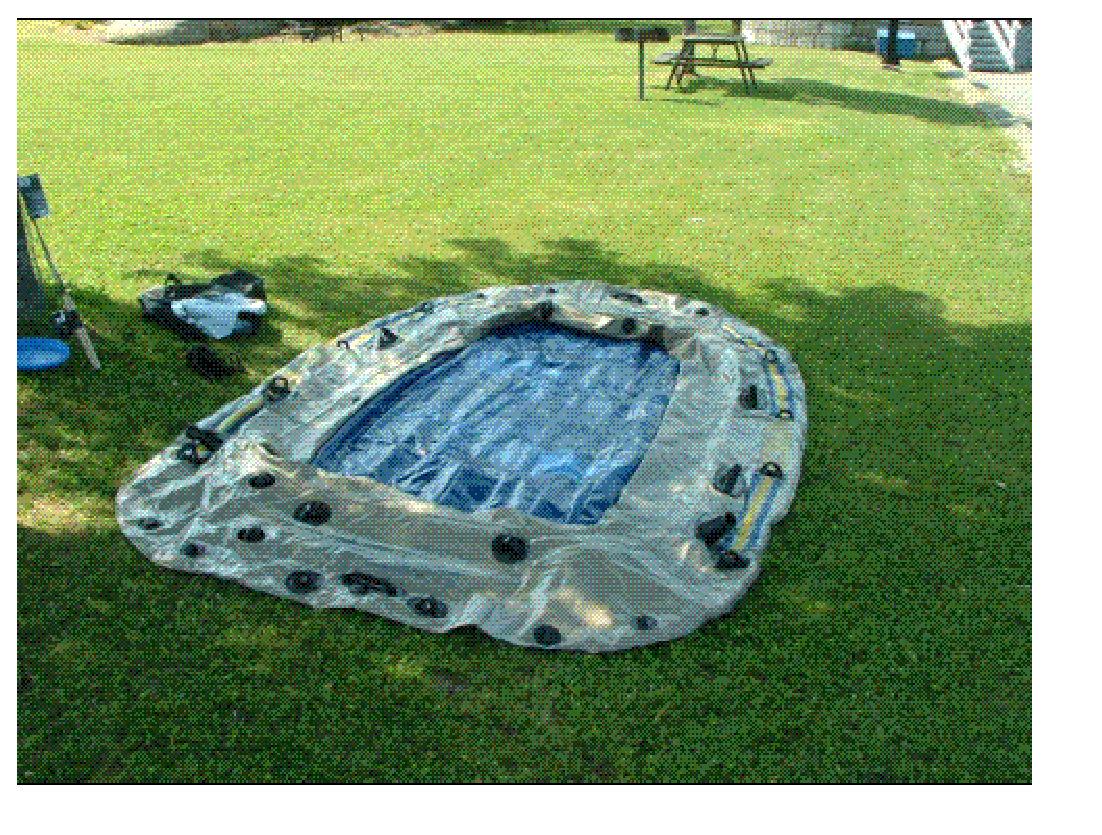
\epsfig{file=fig1.eps,width=3.5in}
Which one of the following is missing in it?
 
 
\noindent{\textbf{\large{
A.}}}
An air-boat
 
 
\noindent{\textbf{\large{
B.}}}
Lawn
 
 
\noindent{\textbf{\large{
C.}}}
A table
 
 
\noindent{\textbf{\large{
D.}}}
A truck
 
 
\noindent{\textbf{\large{
E.}}}
An airplane
 
 
\noindent{\textbf{\large{
F.}}}
  Not any of aboves.
 
 
\noindent\vspace{0.05in}{\textbf{\Large{Auto-answer:}}}
 
 
\noindent{\textbf{\large{
D.}}}
A truck
 
 
\noindent{\textbf{\large{
E.}}}
An airplane
 
 
\noindent\vspace{0.05in}{\textbf{\Large{End of auto-answer.}}}
 
 
 
\vspace{0.3in}
   
   
\noindent{\textbf{\Large{Total numbers: }}}
   
   
\noindent\begin{tabular}{|l|l|l|l|l|l|l|}
 \hline
Inputs & Calculates & Choices & Layers & Matches & Answer & Solution \\ \hline
           0  & 
           0  & 
           6
  simple  
  & 
           6  & 
           0  & 
  yes & 
  no 
  \\ \hline
 \end{tabular}
   
   
   
   
\noindent\vspace{0.1in}{\textbf{\Large{Calculated values:}}}
   
   
   
   
\noindent\vspace{0.1in}\hspace{-0.08in} {\textbf{\Large{All inputs: }}}
   
   
  
\vspace{0.2in}
  
{\textbf{\Large{Question
26.1.2 
 (           6 ,          11 ,          26 )
}}}
  
  
In a hotel, the possiblity of  % 
non-smoking customer is
$a =  % 
0.270$, and the possiblity of  % 
equal or above 30 years old customer is $ b =  % 
0.5200$.
Please calculate the possiblity of  % 
smoking and  % 
under 30 years old customer.
 
 
 
\noindent\vspace{0.1in}{\textbf{\Large{Solution: }}}
 
 

Since the possiblity of  % 
 non-smoking customer is $ a =  % 
0.270 $,
and the possiblity of  % 
equal or above 30 years old customer is $ b =  % 
0.5200 $,
the possiblity of  % 
smoking customer is $ c = 1.0 - a = 1.0 -
0.270
=  % 
0.730 $ and the possiblity of  % 
under 30 years old
customer is $ d = 1.0 - b = 1.0 -  % 
0.5200 =  % 
0.4800  $.
So the possibility of  % 
smoking and  % 
under 30 years old
customer is $ c \times d =  % 
0.350 $.
 
 
 
\noindent\vspace{0.1in}{\textbf{\Large{End of Solution.}}}
 
 

 
 
 
\noindent\vspace{0.05in}{\textbf{\Large{Answer:}}}
 
 

The possibility of  % 
smoking and  % 
under 30 years old
customer is $ (1-a)(1-b) =  % 
0.350 $.
 
 
\noindent\vspace{0.05in}{\textbf{\Large{End of Answer.}}}
 
 

 
\vspace{0.3in}
   
   
\noindent{\textbf{\Large{Total numbers: }}}
   
   
\noindent\begin{tabular}{|l|l|l|l|l|l|l|}
 \hline
Inputs & Calculates & Choices & Layers & Matches & Answer & Solution \\ \hline
           4  & 
           3  & 
           0
  & 
           0  & 
           0  & 
  yes & 
  yes 
  \\ \hline
 \end{tabular}
   
   
   
   
\noindent\vspace{0.1in}{\textbf{\Large{Calculated values:}}}
   
   
  
  
\noindent\begin{tabular}{|l|l|l|l|}
\hline
 Sequential & Type & Accuracy & Calculated \\ 
\hline
 
 
  Calculated $            1 $ & real & $            3  $ & 
 $ 0.730 $ 
 \\  \hline  
 
 
  Calculated $            2 $ & real & $            4  $ & 
 $ 0.4800 $ 
 \\  \hline  
 
 
  Calculated $            3 $ & real & $            3  $ & 
 $ 0.350 $ 
 \\  \hline  
 \end{tabular}
   
   
   
   
\noindent\vspace{0.1in}\hspace{-0.08in} {\textbf{\Large{All inputs: }}}
   
   
  
  
\noindent\begin{tabular}{|l|l|l|l|l|}
\hline
 Sequential & Type & Accuracy & Three inputs & Generated \\ 
\hline
 
 
  INPUT $            1 $ & logical & .TRUE. & 
 smoking & 
  \\
  & & .FALSE. & 
  non-smoking & 
  $ <-- $ 
 \\  \hline  
 
 
  INPUT $            2 $ & real & $           -3  $ & $
 1.0 \times 10^{-2}
  $ & \\
  & & &  $
 1.000
  $ & \\
  & & &  $
 1.0 \times 10^{-2}
 $ & $ 0.270 $ 
 \\  \hline  
 
 
  INPUT $            3 $ & logical & .TRUE. & 
 equal or above 30 years old & 
  $ <-- $ 
  \\
  & & .FALSE. & 
  under 30 years old & 
 \\  \hline  
 \end{tabular}
   
   
  
  
\noindent\begin{tabular}{|l|l|l|l|l|}
\hline
 Sequential & Type & Accuracy & Three inputs & Generated \\ 
\hline
 
 
  INPUT $            4 $ & real & $           -4  $ & $
 2.00 \times 10^{-2}
  $ & \\
  & & &  $
 1.0000
  $ & \\
  & & &  $
 2.00 \times 10^{-2}
 $ & $ 0.5200 $ 
 \\  \hline  
 \end{tabular}
   
   
  
\vspace{0.2in}
  
{\textbf{\Large{Question
26.1.3 
 (           6 ,          13 ,          28 )
}}}
  
  
What is the operation between $a= % 
3$ and $b= % 
2$:
$a$  % 
$+$ $b=?$ Please also calculate it.
 
 
\noindent\vspace{0.05in}{\textbf{\Large{Answer:}}}
 
 

3;
 
2;
 
The operation is  % 
ADDITION and the result is
$ % 
5.0000$.
 
 
 
\noindent\vspace{0.05in}{\textbf{\Large{End of Answer.}}}
 
 

 
\vspace{0.3in}
   
   
\noindent{\textbf{\Large{Total numbers: }}}
   
   
\noindent\begin{tabular}{|l|l|l|l|l|l|l|}
 \hline
Inputs & Calculates & Choices & Layers & Matches & Answer & Solution \\ \hline
           3  & 
           2  & 
           0
  & 
           0  & 
           0  & 
  yes & 
  no 
  \\ \hline
 \end{tabular}
   
   
   
   
\noindent\vspace{0.1in}{\textbf{\Large{Calculated values:}}}
   
   
  
  
\noindent\begin{tabular}{|l|l|l|l|}
\hline
 Sequential & Type & Accuracy & Calculated \\ 
\hline
 
 
  Calculated $            1 $ & string & $            1  $ ( $           1  $ strings): 
 & ADDITION
 \\  \hline  
 
 
  Calculated $            2 $ & real & $            5  $ & 
 $ 5.0000 $ 
 \\  \hline  
 \end{tabular}
   
   
   
   
\noindent\vspace{0.1in}\hspace{-0.08in} {\textbf{\Large{All inputs: }}}
   
   
  
  
\noindent\begin{tabular}{|l|l|l|l|l|}
\hline
 Sequential & Type & Accuracy & Three inputs & Generated \\ 
\hline
 
 
  INPUT $            1 $ & integer &  & $
 1
 , 
 10
 , 
 2
 $ & $ 3 $ 
 \\  \hline  
 
 
  INPUT $            2 $ & integer &  & $
 2
 , 
 10
 , 
 2
 $ & $ 2 $ 
 \\  \hline  
 
 
  INPUT $            3 $ & string & & 
 $+$ & 
  $ <-- $ 
  \\
  & & & 
 $-$ & 
  \\
  & & & 
 $\times$ & 
  \\
  & & & 
 $\div$ & 
 \\  \hline  
 \end{tabular}
   
   
  
\vspace{0.2in}
  
{\textbf{\Large{Question
26.1.4 
 (           6 ,           9 ,          24 )
}}}
  
  
Let us use Newton's Law of Universal Gravitation to calculate the force
of the Sun acting on the eight planets. Let us suppose the mass of the
Sun is $ % 
7.00 \times 10^{24} kg$. With the mass and the
distance to the Sun of each planet in the following table, please fill
the blanks for the forces.
 
\vspace{0.2in}
 
 
\begin{tabular}{|l|l|l|l|}
\hline
The Planet & Mass ($kg$) & Distanace from Sun ($m$) & The Force ($N$)\\
\hline
Mercury  &
           $ % 
2.00000000 \times 10^{24} $   &
             $ % 
5.000000000 \times 10^{24} $    &
\\  \hline
Venus    &
           $ % 
8.00 \times 10^{24} $    &
             $ % 
6.00 \times 10^{24} $    &
\\  \hline
Earth    &
           $ % 
9.00 \times 10^{24} $    &
             $ % 
3.00 \times 10^{24} $    &
\\   \hline
Mars     &
           $ % 
9.00 \times 10^{24} $    &
             $ % 
4.00 \times 10^{24} $    &
\\   \hline
Jupiter  &
           $ % 
2.00 \times 10^{24} $    &
             $ % 
3.00 \times 10^{24} $    &
\\  \hline
Saturn   &
           $ % 
9.00 \times 10^{24}$    &
             $ % 
6.00 \times 10^{24}$    &
\\  \hline
Uranus   &
           $ % 
8.00 \times 10^{24} $    &
             $ % 
7.00 \times 10^{24} $    &
\\  \hline
Neptune  &
           $ % 
5.00 \times 10^{24} $    &
             $ % 
4.00 \times 10^{24} $    &
\\  \hline
 
\end{tabular}
 
 
 
 
\noindent\vspace{0.1in}{\textbf{\Large{Solution: }}}
 
 

By using Newton's Law of Universal Gravitation:
\[
F=G \frac{(Sun's \hspace{0.1in} mass) \times (Planet's \hspace{0.1in} mass)} { (distance)^2},
\]
where
$ G= % 
6.67 \times 10^{-11}N m^{2}(kg)^{-2}$ , the forces can be easily calculated as
 
\vspace{0.2in}
 
 
\begin{tabular}{|l|l|l|l|}
\hline
The Planet & Mass ($kg$) & Distanace from Sun ($m$) & The Force ($N$)\\
\hline
Mercury  &
           $ % 
2.00000000 \times 10^{24} $   &
             $ % 
5.000000000 \times 10^{24} $    & $ % 
3.74 \times 10^{-11} $
\\  \hline
Venus    &
           $  % 
8.00 \times 10^{24}  $     &
             $ % 
6.00 \times 10^{24} $    & $ % 
1.04 \times 10^{-10} $
\\  \hline
Earth    &
           $  % 
9.00 \times 10^{24}  $     &
             $ % 
3.00 \times 10^{24} $    & $ % 
4.67 \times 10^{-10} $
\\   \hline
Mars     &
           $  % 
9.00 \times 10^{24} $     &
             $ % 
4.00 \times 10^{24} $    & $ % 
2.63 \times 10^{-10} $
\\   \hline
Jupiter  &
           $  % 
2.00 \times 10^{24} $    &
             $ % 
3.00 \times 10^{24} $    & $ % 
1.04 \times 10^{-10} $
\\  \hline
Saturn   &
           $  % 
9.00 \times 10^{24} $    &
             $ % 
6.00 \times 10^{24}  $    & $ % 
1.17 \times 10^{-10} $
\\  \hline
Uranus   &
           $  % 
8.00 \times 10^{24} $    &
             $ % 
7.00 \times 10^{24} $    & $ % 
7.62 \times 10^{-11} $
\\  \hline
Neptune  &
           $  % 
5.00 \times 10^{24} $    &
             $ % 
4.00 \times 10^{24} $    & $ % 
1.46 \times 10^{-10} $
\\  \hline
 
\end{tabular}
 
 
 
 
\noindent\vspace{0.1in}{\textbf{\Large{End of Solution.}}}
 
 

 
 
 
 
\noindent\vspace{0.05in}{\textbf{\Large{Answer:}}}
 
 

By using Newton's Law of Universal Gravitation:
\[
F=G \frac{(Sun's \hspace{0.1in} mass) \times (Planet's \hspace{0.1in} mass)} { (distance)^2},
\]
where
$ G= % 
6.67 \times 10^{-11} N m^{2}(kg)^{-2}$ , the forces can be easily calculated as
 
\vspace{0.2in}
 
 
\begin{tabular}{|l|l|l|l|}
\hline
The Planet & Mass ($kg$) & Distanace from Sun ($m$) & The Force ($N$)\\
\hline
Mercury  &
           $ % 
2.00000000 \times 10^{24}  $   &
             $ % 
5.000000000 \times 10^{24}$    & $ % 
3.74 \times 10^{-11} $
\\  \hline
Venus    &
           $  % 
8.00 \times 10^{24}  $     &
             $ % 
6.00 \times 10^{24} $    & $ % 
1.04 \times 10^{-10} $
\\  \hline
Earth    &
           $  % 
9.00 \times 10^{24}$     &
             $ % 
3.00 \times 10^{24} $    & $ % 
4.67 \times 10^{-10} $
\\   \hline
Mars     &
           $  % 
9.00 \times 10^{24} $     &
             $ % 
4.00 \times 10^{24}$    & $ % 
2.63 \times 10^{-10} $
\\   \hline
Jupiter  &
           $  % 
2.00 \times 10^{24}  $    &
             $ % 
3.00 \times 10^{24} $    & $ % 
1.04 \times 10^{-10}3 $
\\  \hline
Saturn   &
           $  % 
9.00 \times 10^{24}   $    &
             $ % 
6.00 \times 10^{24}  $    & $ % 
1.17 \times 10^{-10} $
\\  \hline
Uranus   &
           $  % 
8.00 \times 10^{24} $    &
             $ % 
7.00 \times 10^{24}$    & $ % 
7.62 \times 10^{-11} $
\\  \hline
Neptune  &
           $  % 
5.00 \times 10^{24}  $    &
             $ % 
4.00 \times 10^{24} $    & $ % 
1.46 \times 10^{-10} $
\\  \hline
 
\end{tabular}
 
 
 
 
\noindent\vspace{0.05in}{\textbf{\Large{End of Answer.}}}
 
 

 
\vspace{0.3in}
   
   
\noindent{\textbf{\Large{Total numbers: }}}
   
   
\noindent\begin{tabular}{|l|l|l|l|l|l|l|}
 \hline
Inputs & Calculates & Choices & Layers & Matches & Answer & Solution \\ \hline
          19  & 
           8  & 
           0
  & 
           0  & 
           0  & 
  yes & 
  yes 
  \\ \hline
 \end{tabular}
   
   
   
   
\noindent\vspace{0.1in}{\textbf{\Large{Calculated values:}}}
   
   
  
  
\noindent\begin{tabular}{|l|l|l|l|}
\hline
 Sequential & Type & Accuracy & Calculated \\ 
\hline
 
 
  Calculated $            1 $ & real & $            3  $ & 
 $ 3.74 \times 10^{-11} $ 
 \\  \hline  
 
 
  Calculated $            2 $ & real & $            3  $ & 
 $ 1.04 \times 10^{-10} $ 
 \\  \hline  
 
 
  Calculated $            3 $ & real & $            3  $ & 
 $ 4.67 \times 10^{-10} $ 
 \\  \hline  
 
 
  Calculated $            4 $ & real & $            3  $ & 
 $ 2.63 \times 10^{-10} $ 
 \\  \hline  
 
 
  Calculated $            5 $ & real & $            3  $ & 
 $ 1.04 \times 10^{-10} $ 
 \\  \hline  
 
 
  Calculated $            6 $ & real & $            3  $ & 
 $ 1.17 \times 10^{-10} $ 
 \\  \hline  
 
 
  Calculated $            7 $ & real & $            3  $ & 
 $ 7.62 \times 10^{-11} $ 
 \\  \hline  
 
 
  Calculated $            8 $ & real & $            3  $ & 
 $ 1.46 \times 10^{-10} $ 
 \\  \hline  
 \end{tabular}
   
   
   
   
\noindent\vspace{0.1in}\hspace{-0.08in} {\textbf{\Large{All inputs: }}}
   
   
  
  
\noindent\begin{tabular}{|l|l|l|l|l|}
\hline
 Sequential & Type & Accuracy & Three inputs & Generated \\ 
\hline
 
 
  INPUT $            1 $ & real & $           22  $ & $
 2.00 \times 10^{24}
  $ & \\
  & & &  $
 1.010 \times 10^{25}
  $ & \\
  & & &  $
 1.00 \times 10^{24}
 $ & $ 7.00 \times 10^{24} $ 
 \\  \hline  
 
 
  INPUT $            2 $ & real & $           16  $ & $
 2.00000000 \times 10^{24}
  $ & \\
  & & &  $
 1.010000000 \times 10^{25}
  $ & \\
  & & &  $
 1.00000000 \times 10^{24}
 $ & $ 2.00000000 \times 10^{24} $ 
 \\  \hline  
 
 
  INPUT $            3 $ & real & $           15  $ & $
 2.000000000 \times 10^{24}
  $ & \\
  & & &  $
 1.0100000000 \times 10^{25}
  $ & \\
  & & &  $
 1.000000000 \times 10^{24}
 $ & $ 5.000000000 \times 10^{24} $ 
 \\  \hline  
 \end{tabular}
   
   
  
  
\noindent\begin{tabular}{|l|l|l|l|l|}
\hline
 Sequential & Type & Accuracy & Three inputs & Generated \\ 
\hline
 
 
  INPUT $            4 $ & real & $           22  $ & $
 2.00 \times 10^{24}
  $ & \\
  & & &  $
 1.010 \times 10^{25}
  $ & \\
  & & &  $
 1.00 \times 10^{24}
 $ & $ 8.00 \times 10^{24} $ 
 \\  \hline  
 
 
  INPUT $            5 $ & real & $           22  $ & $
 2.00 \times 10^{24}
  $ & \\
  & & &  $
 1.010 \times 10^{25}
  $ & \\
  & & &  $
 1.00 \times 10^{24}
 $ & $ 6.00 \times 10^{24} $ 
 \\  \hline  
 
 
  INPUT $            6 $ & real & $           22  $ & $
 2.00 \times 10^{24}
  $ & \\
  & & &  $
 1.010 \times 10^{25}
  $ & \\
  & & &  $
 1.00 \times 10^{24}
 $ & $ 9.00 \times 10^{24} $ 
 \\  \hline  
 \end{tabular}
   
   
  
  
\noindent\begin{tabular}{|l|l|l|l|l|}
\hline
 Sequential & Type & Accuracy & Three inputs & Generated \\ 
\hline
 
 
  INPUT $            7 $ & real & $           22  $ & $
 2.00 \times 10^{24}
  $ & \\
  & & &  $
 1.010 \times 10^{25}
  $ & \\
  & & &  $
 1.00 \times 10^{24}
 $ & $ 3.00 \times 10^{24} $ 
 \\  \hline  
 
 
  INPUT $            8 $ & real & $           22  $ & $
 2.00 \times 10^{24}
  $ & \\
  & & &  $
 1.010 \times 10^{25}
  $ & \\
  & & &  $
 1.00 \times 10^{24}
 $ & $ 9.00 \times 10^{24} $ 
 \\  \hline  
 
 
  INPUT $            9 $ & real & $           22  $ & $
 2.00 \times 10^{24}
  $ & \\
  & & &  $
 1.010 \times 10^{25}
  $ & \\
  & & &  $
 1.00 \times 10^{24}
 $ & $ 4.00 \times 10^{24} $ 
 \\  \hline  
 \end{tabular}
   
   
  
  
\noindent\begin{tabular}{|l|l|l|l|l|}
\hline
 Sequential & Type & Accuracy & Three inputs & Generated \\ 
\hline
 
 
  INPUT $           10 $ & real & $           22  $ & $
 2.00 \times 10^{24}
  $ & \\
  & & &  $
 1.010 \times 10^{25}
  $ & \\
  & & &  $
 1.00 \times 10^{24}
 $ & $ 2.00 \times 10^{24} $ 
 \\  \hline  
 
 
  INPUT $           11 $ & real & $           22  $ & $
 2.00 \times 10^{24}
  $ & \\
  & & &  $
 1.010 \times 10^{25}
  $ & \\
  & & &  $
 1.00 \times 10^{24}
 $ & $ 3.00 \times 10^{24} $ 
 \\  \hline  
 
 
  INPUT $           12 $ & real & $           22  $ & $
 2.00 \times 10^{24}
  $ & \\
  & & &  $
 1.010 \times 10^{25}
  $ & \\
  & & &  $
 1.00 \times 10^{24}
 $ & $ 9.00 \times 10^{24} $ 
 \\  \hline  
 \end{tabular}
   
   
  
  
\noindent\begin{tabular}{|l|l|l|l|l|}
\hline
 Sequential & Type & Accuracy & Three inputs & Generated \\ 
\hline
 
 
  INPUT $           13 $ & real & $           22  $ & $
 2.00 \times 10^{24}
  $ & \\
  & & &  $
 1.010 \times 10^{25}
  $ & \\
  & & &  $
 1.00 \times 10^{24}
 $ & $ 6.00 \times 10^{24} $ 
 \\  \hline  
 
 
  INPUT $           14 $ & real & $           22  $ & $
 2.00 \times 10^{24}
  $ & \\
  & & &  $
 1.010 \times 10^{25}
  $ & \\
  & & &  $
 1.00 \times 10^{24}
 $ & $ 8.00 \times 10^{24} $ 
 \\  \hline  
 
 
  INPUT $           15 $ & real & $           22  $ & $
 2.00 \times 10^{24}
  $ & \\
  & & &  $
 1.010 \times 10^{25}
  $ & \\
  & & &  $
 1.00 \times 10^{24}
 $ & $ 7.00 \times 10^{24} $ 
 \\  \hline  
 \end{tabular}
   
   
  
  
\noindent\begin{tabular}{|l|l|l|l|l|}
\hline
 Sequential & Type & Accuracy & Three inputs & Generated \\ 
\hline
 
 
  INPUT $           16 $ & real & $           22  $ & $
 2.00 \times 10^{24}
  $ & \\
  & & &  $
 1.010 \times 10^{25}
  $ & \\
  & & &  $
 1.00 \times 10^{24}
 $ & $ 5.00 \times 10^{24} $ 
 \\  \hline  
 
 
  INPUT $           17 $ & real & $           22  $ & $
 2.00 \times 10^{24}
  $ & \\
  & & &  $
 1.010 \times 10^{25}
  $ & \\
  & & &  $
 1.00 \times 10^{24}
 $ & $ 4.00 \times 10^{24} $ 
 \\  \hline  
 
 
  INPUT $           18 $ & real & $          -13  $ & $
 6.67 \times 10^{-11}
  $ & \\
  & & &  $
 6.67 \times 10^{-11}
  $ & \\
  & & &  $
 1.00 \times 10^{-11}
 $ & $ 6.67 \times 10^{-11} $ 
 \\  \hline  
 \end{tabular}
   
   
  
  
\noindent\begin{tabular}{|l|l|l|l|l|}
\hline
 Sequential & Type & Accuracy & Three inputs & Generated \\ 
\hline
 
 
  INPUT $           19 $ & real & $          -13  $ & $
 6.67 \times 10^{-11}
  $ & \\
  & & &  $
 6.67 \times 10^{-11}
  $ & \\
  & & &  $
 1.00 \times 10^{-11}
 $ & $ 6.67 \times 10^{-11} $ 
 \\  \hline  
 \end{tabular}
   
   
  
\vspace{0.2in}
  
{\textbf{\Large{Question
26.1.5 
 (           6 ,           8 ,          23 )
}}}
  
  
 
An object is subjected to an external net force $\mathbf{f}=(
80.0 ,
3.0,
-3000.0  )N$. Its mass is known as
$m= % 
52.0  kg$. Please choose the correct accelaration
from the following choices.
 
 
 
\noindent{\textbf{\large{
A.}}}
The accelaration is
$(
6.6592ms^{-2},
5.7692 \times 10^{-2}ms^{-2},
-2.5735 \times 10^{6}km/h^2
).
$
 
 
\noindent{\textbf{\large{
B.}}}
The accelaration is
$(
6.6592ms^{-2},
-0.12162ms^{-2},
-2.5735 \times 10^{6}km/h^2
).
$
 
 
\noindent{\textbf{\large{
C.}}}
The accelaration is
$(
6.6592ms^{-2},
5.7692 \times 10^{-2}ms^{-2},
-747692.km/h^2
).
$
 
 
\noindent{\textbf{\large{
D.}}}
The accelaration is
$(
1.5385ms^{-2},
5.7692 \times 10^{-2}ms^{-2},
-747692.km/h^2
).
$
 
 
\noindent{\textbf{\large{
E.}}}
none of these.
 
 
\noindent\vspace{0.05in}{\textbf{\Large{Auto-answer:}}}
 
 
\noindent{\textbf{\large{
D.}}}
The accelaration is
$(
1.5385ms^{-2},
5.7692 \times 10^{-2}ms^{-2},
-747692.km/h^2
).
$
 
 
\noindent\vspace{0.05in}{\textbf{\Large{End of auto-answer.}}}
 
 
 
 
 
 
\noindent\vspace{0.1in}{\textbf{\Large{Solution: }}}
 
 

We will use the Newton's Second Law:
 
\[
\mathbf{f}=m\mathbf{a}.
\]
 
Since $\mathbf{f}=( % 
80.0,  % 
3.0,  % 
-3000.0 )N$
and $m= % 
52.0kg$, bring them into the above equation, then we get
 
\begin{eqnarray*}
\mathbf{a}&=&\frac{\mathbf{f}}m  \\
&=&\frac{(
80.0 ,
3.0 ,
-3000.0 )N
}{ % 
52.0 kg}  \\
&=&(
1.5385 ,
5.7692 \times 10^{-2},
-57.692
)ms^{-2} \\
&=&(
19938. ,
747.69 ,
-747692.
)km/h^2.
\end{eqnarray*}
 
 
 
\noindent\vspace{0.1in}{\textbf{\Large{End of Solution.}}}
 
 

 
\vspace{0.3in}
   
   
\noindent{\textbf{\Large{Total numbers: }}}
   
   
\noindent\begin{tabular}{|l|l|l|l|l|l|l|}
 \hline
Inputs & Calculates & Choices & Layers & Matches & Answer & Solution \\ \hline
           4  & 
           6  & 
           5
  & 
           3  & 
           0  & 
  yes & 
  yes 
  \\ \hline
 \end{tabular}
   
   
   
   
\noindent\vspace{0.1in}{\textbf{\Large{Calculated values:}}}
   
   
  
  
\noindent\begin{tabular}{|l|l|l|l|}
\hline
 Sequential & Type & Accuracy & Calculated \\ 
\hline
 
 
  Calculated $            1 $ & real & $            5  $ & 
 $ 1.5385 $ 
 \\  \hline  
 
 
  Calculated $            2 $ & real & $            5  $ & 
 $ 5.7692 \times 10^{-2} $ 
 \\  \hline  
 
 
  Calculated $            3 $ & real & $            5  $ & 
 $ -57.692 $ 
 \\  \hline  
 
 
  Calculated $            4 $ & real & $            5  $ & 
 $ 19938. $ 
 \\  \hline  
 
 
  Calculated $            5 $ & real & $            5  $ & 
 $ 747.69 $ 
 \\  \hline  
 
 
  Calculated $            6 $ & real & $            5  $ & 
 $ -747692. $ 
 \\  \hline  
 \end{tabular}
   
   
   
   
\noindent\vspace{0.1in}\hspace{-0.08in} {\textbf{\Large{All inputs: }}}
   
   
  
  
\noindent\begin{tabular}{|l|l|l|l|l|}
\hline
 Sequential & Type & Accuracy & Three inputs & Generated \\ 
\hline
 
 
  INPUT $            1 $ & real & $           -1  $ & $
 20.0
  $ & \\
  & & &  $
 101.0
  $ & \\
  & & &  $
 10.0
 $ & $ 80.0 $ 
 \\  \hline  
 
 
  INPUT $            2 $ & real & $           -1  $ & $
 2.0
  $ & \\
  & & &  $
 10.1
  $ & \\
  & & &  $
 1.0
 $ & $ 3.0 $ 
 \\  \hline  
 
 
  INPUT $            3 $ & real & $           -1  $ & $
 -2000.0
  $ & \\
  & & &  $
 -10001.0
  $ & \\
  & & &  $
 -1000.0
 $ & $ -3000.0 $ 
 \\  \hline  
 \end{tabular}
   
   
  
  
\noindent\begin{tabular}{|l|l|l|l|l|}
\hline
 Sequential & Type & Accuracy & Three inputs & Generated \\ 
\hline
 
 
  INPUT $            4 $ & real & $           -1  $ & $
 50.0
  $ & \\
  & & &  $
 60.1
  $ & \\
  & & &  $
 2.0
 $ & $ 52.0 $ 
 \\  \hline  
 \end{tabular}
   
   
  
\vspace{0.2in}
  
{\textbf{\Large{Question
26.1.6 
 (           6 ,           7 ,          22 )
}}}
  
  
 
An object is subjected to an external net force $\mathbf{f}=(
90.0 ,
2.0,
-7000.0  )N$. Its mass is known as
$m= % 
56.0  kg$. Please choose the correct accelaration
from the following choices.
 
 
 
\noindent{\textbf{\large{
A.}}}
The accelaration (vector) is
$(
-103670.,
462.86 ,
4.9517 \times 10^{6}
)km/h^2.
$
 
 
\noindent{\textbf{\large{
B.}}}
The accelaration (vector) is
$(
55447.,
462.86 ,
6.8897 \times 10^{6}
)km/h^2.
$
 
 
\noindent{\textbf{\large{
C.}}}
The accelaration (vector) is
$(
55447.,
462.86 ,
-1.6200 \times 10^{6}
)km/h^2.
$
 
 
\noindent{\textbf{\large{
D.}}}
The accelaration (vector) is
$(
20829.,
462.86 ,
-1.6200 \times 10^{6}
)km/h^2.
$
 
 
\noindent{\textbf{\large{
E.}}}
The accelaration (vector) is
$(
20829.,
462.86 ,
6.8897 \times 10^{6}
)km/h^2.
$
 
 
\noindent{\textbf{\large{
F.}}}
The accelaration (vector) is
$(
-103670.,
462.86 ,
6.8897 \times 10^{6}
)km/h^2.
$
 
 
\noindent{\textbf{\large{
G.}}}
The accelaration (vector) is
$(
20829.,
462.86 ,
4.1819 \times 10^{6}
)km/h^2.
$
 
 
\noindent{\textbf{\large{
H.}}}
The accelaration (vector) is
$(
71153.,
462.86 ,
4.1819 \times 10^{6}
)km/h^2.
$
 
 
\noindent{\textbf{\large{
I.}}}
The accelaration (vector) is
$(
55447.,
462.86 ,
4.9517 \times 10^{6}
)km/h^2.
$
 
 
\noindent{\textbf{\large{
J.}}}
The accelaration (vector) is
$(
-103670.,
462.86 ,
4.1819 \times 10^{6}
)km/h^2.
$
 
 
\noindent{\textbf{\large{
K.}}}
The accelaration (vector) is
$(
71153.,
462.86 ,
4.9517 \times 10^{6}
)km/h^2.
$
 
 
\noindent{\textbf{\large{
L.}}}
The accelaration (vector) is
$(
-103670.,
462.86 ,
-1.6200 \times 10^{6}
)km/h^2.
$
 
 
\noindent\vspace{0.05in}{\textbf{\Large{Auto-answer:}}}
 
 
\noindent{\textbf{\large{
D.}}}
The accelaration (vector) is
$(
20829.,
462.86 ,
-1.6200 \times 10^{6}
)km/h^2.
$
 
 
\noindent\vspace{0.05in}{\textbf{\Large{End of auto-answer.}}}
 
 
 
 
 
 
\noindent\vspace{0.1in}{\textbf{\Large{Solution: }}}
 
 

We will use the Newton's Second Law:
 
\[
\mathbf{f}=m\mathbf{a}.
\]
 
Since $\mathbf{f}=( % 
90.0,  % 
2.0,  % 
-7000.0 )N$
and $m= % 
56.0 kg$, bring them into the above equation, then we get
 
\begin{eqnarray*}
\mathbf{a}&=&\frac{\mathbf{f}}m  \\
&=&\frac{(
90.0 ,
2.0 ,
-7000.0 )N
}{ % 
56.0 kg}  \\
&=&(
1.6071 ,
3.5714 \times 10^{-2},
-125.00
)ms^{-2} \\
&=&(
20829. ,
462.86 ,
-1.6200 \times 10^{6}
)km/h^2.
\end{eqnarray*}
 
 
 
\noindent\vspace{0.1in}{\textbf{\Large{End of Solution.}}}
 
 

 
 
\vspace{0.3in}
   
   
\noindent{\textbf{\Large{Total numbers: }}}
   
   
\noindent\begin{tabular}{|l|l|l|l|l|l|l|}
 \hline
Inputs & Calculates & Choices & Layers & Matches & Answer & Solution \\ \hline
           4  & 
           6  & 
          12
  & 
           2  & 
           0  & 
  yes & 
  yes 
  \\ \hline
 \end{tabular}
   
   
   
   
\noindent\vspace{0.1in}{\textbf{\Large{Calculated values:}}}
   
   
  
  
\noindent\begin{tabular}{|l|l|l|l|}
\hline
 Sequential & Type & Accuracy & Calculated \\ 
\hline
 
 
  Calculated $            1 $ & real & $            5  $ & 
 $ 1.6071 $ 
 \\  \hline  
 
 
  Calculated $            2 $ & real & $            5  $ & 
 $ 3.5714 \times 10^{-2} $ 
 \\  \hline  
 
 
  Calculated $            3 $ & real & $            5  $ & 
 $ -125.00 $ 
 \\  \hline  
 
 
  Calculated $            4 $ & real & $            5  $ & 
 $ 20829. $ 
 \\  \hline  
 
 
  Calculated $            5 $ & real & $            5  $ & 
 $ 462.86 $ 
 \\  \hline  
 
 
  Calculated $            6 $ & real & $            5  $ & 
 $ -1.6200 \times 10^{6} $ 
 \\  \hline  
 \end{tabular}
   
   
   
   
\noindent\vspace{0.1in}\hspace{-0.08in} {\textbf{\Large{All inputs: }}}
   
   
  
  
\noindent\begin{tabular}{|l|l|l|l|l|}
\hline
 Sequential & Type & Accuracy & Three inputs & Generated \\ 
\hline
 
 
  INPUT $            1 $ & real & $           -1  $ & $
 20.0
  $ & \\
  & & &  $
 101.0
  $ & \\
  & & &  $
 10.0
 $ & $ 90.0 $ 
 \\  \hline  
 
 
  INPUT $            2 $ & real & $           -1  $ & $
 2.0
  $ & \\
  & & &  $
 10.1
  $ & \\
  & & &  $
 1.0
 $ & $ 2.0 $ 
 \\  \hline  
 
 
  INPUT $            3 $ & real & $           -1  $ & $
 -2000.0
  $ & \\
  & & &  $
 -10001.0
  $ & \\
  & & &  $
 -1000.0
 $ & $ -7000.0 $ 
 \\  \hline  
 \end{tabular}
   
   
  
  
\noindent\begin{tabular}{|l|l|l|l|l|}
\hline
 Sequential & Type & Accuracy & Three inputs & Generated \\ 
\hline
 
 
  INPUT $            4 $ & real & $           -1  $ & $
 50.0
  $ & \\
  & & &  $
 60.1
  $ & \\
  & & &  $
 2.0
 $ & $ 56.0 $ 
 \\  \hline  
 \end{tabular}
   
   
   
   
\vspace{0.3in}
{\textbf{\LARGE{You have done all the above? A very good beginning, please go ahead.}}}
More constants the
Mass of electron
$m_e$$ =
9.109390 \times 10^{-31} $
kg
,
Universal gas constant
$R$$ =
8.315 $
J/(mol$\cdot $K)
,
$e$$ =
1.60217733 \times 10^{-19} $
C
, and
$m_p$$ =
1.6726231 \times 10^{-27} $
kg
%
may be very helpful.
\vspace{0.3in}
   
   
  
\vspace{0.2in}
  
{\textbf{\Large{QUESTION
26.2 
 (           5 ,           5 ,           5 )
}}}
  
  
If any one of the following statements is correct, please fill the box ahead of it with $T$ .
If wrong, fill with $F$.
 
\noindent\begin{tabular}{|l|l|}\hline Your&\hspace{.2in} \\ answer&\hspace{.2in} \\ \hline \end{tabular}
1. $ % 
96$ is an  % 
even number.
 
\noindent\begin{tabular}{|l|l|}\hline Your&\hspace{.2in} \\ answer&\hspace{.2in} \\ \hline \end{tabular}
2.  % 
Toronto is in  % 
Ontario province.
 
\noindent\begin{tabular}{|l|l|}\hline Your&\hspace{.2in} \\ answer&\hspace{.2in} \\ \hline \end{tabular}
3.  % 
$\left| \mathbf{F}\right| =Gm_1m_2r^{-2}$ is a mathmatical form of
the Newton's Second Law.
 
 
 
\noindent\vspace{0.05in}{\textbf{\Large{Answer:}}}
 
 

 
\noindent\begin{tabular}{|l|l|}\hline The correct & \\
          answer &  % 
$T$ \\ \hline \end{tabular}
1. $ % 
96$ is an  % 
even number.
 
\noindent\begin{tabular}{|l|l|}\hline The correct & \\
          answer &  % 
$T$ \\ \hline \end{tabular}
2.  % 
Toronto is in  % 
Ontario province.
 
\noindent\begin{tabular}{|l|l|}\hline The correct & \\
          answer &  % 
$F$ \\ \hline \end{tabular}
3.  % 
$\left| \mathbf{F}\right| =Gm_1m_2r^{-2}$ is a mathmatical form of  % 
the Newton's Second Law.
 
 
 
\noindent\vspace{0.05in}{\textbf{\Large{End of Answer.}}}
 
 

 
\vspace{0.3in}
   
   
\noindent{\textbf{\Large{Total numbers: }}}
   
   
\noindent\begin{tabular}{|l|l|l|l|l|l|l|}
 \hline
Inputs & Calculates & Choices & Layers & Matches & Answer & Solution \\ \hline
           6  & 
           3  & 
           0
  & 
           0  & 
           0  & 
  yes & 
  no 
  \\ \hline
 \end{tabular}
   
   
   
   
\noindent\vspace{0.1in}{\textbf{\Large{Calculated values:}}}
   
   
  
  
\noindent\begin{tabular}{|l|l|l|l|}
\hline
 Sequential & Type & Accuracy & Calculated \\ 
\hline
 
 
  Calculated $            1 $ & string & $            1  $ ( $           1  $ strings): 
 & $T$
 \\  \hline  
 
 
  Calculated $            2 $ & string & $            1  $ ( $           1  $ strings): 
 & $T$
 \\  \hline  
 
 
  Calculated $            3 $ & string & $            1  $ ( $           1  $ strings): 
 & $F$
 \\  \hline  
 \end{tabular}
   
   
   
   
\noindent\vspace{0.1in}\hspace{-0.08in} {\textbf{\Large{All inputs: }}}
   
   
  
  
\noindent\begin{tabular}{|l|l|l|l|l|}
\hline
 Sequential & Type & Accuracy & Three inputs & Generated \\ 
\hline
 
 
  INPUT $            1 $ & integer &  & $
 1
 , 
 100
 , 
 1
 $ & $ 96 $ 
 \\  \hline  
 
 
  INPUT $            2 $ & string & & 
 even & 
  $ <-- $ 
  \\
  & & & 
 odd & 
 \\  \hline  
 
 
  INPUT $            3 $ & string & & 
 Toronto & 
  $ <-- $ 
  \\
  & & & 
 Kingston & 
  \\
  & & & 
 Montreal & 
  \\
  & & & 
 Hull & 
 \\  \hline  
 \end{tabular}
   
   
  
  
\noindent\begin{tabular}{|l|l|l|l|l|}
\hline
 Sequential & Type & Accuracy & Three inputs & Generated \\ 
\hline
 
 
  INPUT $            4 $ & string & & 
 Ontario & 
  $ <-- $ 
  \\
  & & & 
 Quebec & 
 \\  \hline  
 
 
  INPUT $            5 $ & string & & 
 $\mathbf{F}=m\mathbf{a}$ & 
  \\
  & & & 
 $\left| \mathbf{F}\right| =Gm_1m_2r^{-2}$ & 
  $ <-- $ 
 \\  \hline  
 
 
  INPUT $            6 $ & string & & 
 the Newton's Second Law & 
  $ <-- $ 
  \\
  & & & 
 Newton's Law of Universal Gravitation & 
 \\  \hline  
 \end{tabular}
   
   
  
\vspace{0.2in}
  
{\textbf{\Large{QUESTION
26.3 
 (           3 ,           3 ,           3 )
}}}
  
  
Please choose the correct one from the following statements:
 
 
\noindent{\textbf{\large{
A.}}}
Canada has  %
34 provinces and  %
39 territories.
 
 
\noindent{\textbf{\large{
B.}}}
Canada has  %
37 provinces and  %
37 territories.
 
 
\noindent{\textbf{\large{
C.}}}
Canada has  %
36 provinces and  %
35 territories.
 
 
\noindent{\textbf{\large{
D.}}}
Canada has  %
33 provinces and  %
38 territories.
 
 
\noindent{\textbf{\large{
E.}}}
Canada has  %
35 provinces and  %
34 territories.
 
 
\noindent{\textbf{\large{
F.}}}
 None of above.
 
 
\noindent\vspace{0.05in}{\textbf{\Large{Auto-answer:}}}
 
 
\noindent{\textbf{\large{
F.}}}
 None of above.
 
 
\noindent\vspace{0.05in}{\textbf{\Large{End of auto-answer.}}}
 
 
   
   
\noindent{\textbf{\Large{Total numbers: }}}
   
   
\noindent\begin{tabular}{|l|l|l|l|l|l|l|}
 \hline
Inputs & Calculates & Choices & Layers & Matches & Answer & Solution \\ \hline
           0  & 
          20  & 
           6
  simple  
  & 
           6  & 
           0  & 
  yes & 
  no 
  \\ \hline
 \end{tabular}
   
   
   
   
\noindent\vspace{0.1in}{\textbf{\Large{Calculated values:}}}
   
   
  
  
\noindent\begin{tabular}{|l|l|l|l|}
\hline
 Sequential & Type & Accuracy & Calculated \\ 
\hline
 
 
  Calculated $            1 $ & integer &  & 
  $ 10 $ 
 \\  \hline  
 
 
  Calculated $            2 $ & integer &  & 
  $ 3 $ 
 \\  \hline  
 
 
  Calculated $            3 $ & integer &  & 
  $ 23 $ 
 \\  \hline  
 
 
  Calculated $            4 $ & integer &  & 
  $ 24 $ 
 \\  \hline  
 
 
  Calculated $            5 $ & integer &  & 
  $ 25 $ 
 \\  \hline  
 
 
  Calculated $            6 $ & integer &  & 
  $ 26 $ 
 \\  \hline  
 
 
  Calculated $            7 $ & integer &  & 
  $ 27 $ 
 \\  \hline  
 
 
  Calculated $            8 $ & integer &  & 
  $ 28 $ 
 \\  \hline  
 
 
  Calculated $            9 $ & integer &  & 
  $ 29 $ 
 \\  \hline  
 
 
  Calculated $           10 $ & integer &  & 
  $ 30 $ 
 \\  \hline  
 \end{tabular}
   
   
  
  
\noindent\begin{tabular}{|l|l|l|l|}
\hline
 Sequential & Type & Accuracy & Calculated \\ 
\hline
 
 
  Calculated $           11 $ & integer &  & 
  $ 31 $ 
 \\  \hline  
 
 
  Calculated $           12 $ & integer &  & 
  $ 32 $ 
 \\  \hline  
 
 
  Calculated $           13 $ & integer &  & 
  $ 33 $ 
 \\  \hline  
 
 
  Calculated $           14 $ & integer &  & 
  $ 34 $ 
 \\  \hline  
 
 
  Calculated $           15 $ & integer &  & 
  $ 35 $ 
 \\  \hline  
 
 
  Calculated $           16 $ & integer &  & 
  $ 36 $ 
 \\  \hline  
 
 
  Calculated $           17 $ & integer &  & 
  $ 37 $ 
 \\  \hline  
 
 
  Calculated $           18 $ & integer &  & 
  $ 38 $ 
 \\  \hline  
 
 
  Calculated $           19 $ & integer &  & 
  $ 39 $ 
 \\  \hline  
 
 
  Calculated $           20 $ & integer &  & 
  $ 40 $ 
 \\  \hline  
 \end{tabular}
   
   
   
   
\noindent\vspace{0.1in}\hspace{-0.08in} {\textbf{\Large{All inputs: }}}
   
   
  
\vspace{0.2in}
  
{\textbf{\Large{QUESTION
26.4 
 (           2 ,           2 ,           2 )
}}}
  
  
 
An object is subjected to an external net force $\mathbf{f}=(
30.000 ,
3.0000,
-9000.0  )N$. Its mass is known as
$m= % 
52.0000  kg$. Please choose the correct accelaration
from the following choices.
 
 
 
\noindent{\textbf{\large{
A.}}}
The accelaration is
$(
-1.9975ms^{-2},
747.69km/h^2,
554.32ms^{-2}
).
$
 
 
\noindent{\textbf{\large{
B.}}}
The accelaration is
$(
-1.9975ms^{-2},
3540.9km/h^2,
-173.08ms^{-2}
).
$
 
 
\noindent{\textbf{\large{
C.}}}
The accelaration is
$(
-1.9975ms^{-2},
3540.9km/h^2,
554.32ms^{-2}
).
$
 
 
\noindent{\textbf{\large{
D.}}}
The accelaration is
$(
0.57692ms^{-2},
3540.9km/h^2,
-173.08ms^{-2}
).
$
 
 
\noindent{\textbf{\large{
E.}}}
The accelaration is
$(
-1.9975ms^{-2},
747.69km/h^2,
-173.08ms^{-2}
).
$
 
 
\noindent{\textbf{\large{
F.}}}
The accelaration is
$(
0.57692ms^{-2},
3540.9km/h^2,
554.32ms^{-2}
).
$
 
 
\noindent{\textbf{\large{
G.}}}
 None of these.
 
 
\noindent\vspace{0.05in}{\textbf{\Large{Auto-answer:}}}
 
 
\noindent{\textbf{\large{
G.}}}
 None of these.
 
 
\noindent\vspace{0.05in}{\textbf{\Large{End of auto-answer.}}}
 
 
 
 
 
 
\noindent\vspace{0.1in}{\textbf{\Large{Solution: }}}
 
 

We will use the Newton's Second Law:
 
\[
\mathbf{f}=m\mathbf{a}.
\]
 
Since $\mathbf{f}=( % 
30.000,  % 
3.0000,  % 
-9000.0 )N$
and $m= % 
52.0000kg$, bring them into the above equation, then we get
 
\begin{eqnarray*}
\mathbf{a}&=&\frac{\mathbf{f}}m  \\
&=&\frac{(
30.000 ,
3.0000 ,
-9000.0 )N
}{ % 
52.0000 kg}  \\
&=&(
0.57692 ,
5.7692 \times 10^{-2},
-173.08
)ms^{-2} \\
&=&(
7476.9 ,
747.69 ,
-2.2431 \times 10^{6}
)km/h^2.
\end{eqnarray*}
 
 
 
\noindent\vspace{0.1in}{\textbf{\Large{End of Solution.}}}
 
 

 
\vspace{0.3in}
   
   
\noindent{\textbf{\Large{Total numbers: }}}
   
   
\noindent\begin{tabular}{|l|l|l|l|l|l|l|}
 \hline
Inputs & Calculates & Choices & Layers & Matches & Answer & Solution \\ \hline
           4  & 
           6  & 
           7
  & 
           3  & 
           0  & 
  yes & 
  yes 
  \\ \hline
 \end{tabular}
   
   
   
   
\noindent\vspace{0.1in}{\textbf{\Large{Calculated values:}}}
   
   
  
  
\noindent\begin{tabular}{|l|l|l|l|}
\hline
 Sequential & Type & Accuracy & Calculated \\ 
\hline
 
 
  Calculated $            1 $ & real & $            5  $ & 
 $ 0.57692 $ 
 \\  \hline  
 
 
  Calculated $            2 $ & real & $            5  $ & 
 $ 5.7692 \times 10^{-2} $ 
 \\  \hline  
 
 
  Calculated $            3 $ & real & $            5  $ & 
 $ -173.08 $ 
 \\  \hline  
 
 
  Calculated $            4 $ & real & $            5  $ & 
 $ 7476.9 $ 
 \\  \hline  
 
 
  Calculated $            5 $ & real & $            5  $ & 
 $ 747.69 $ 
 \\  \hline  
 
 
  Calculated $            6 $ & real & $            5  $ & 
 $ -2.2431 \times 10^{6} $ 
 \\  \hline  
 \end{tabular}
   
   
   
   
\noindent\vspace{0.1in}\hspace{-0.08in} {\textbf{\Large{All inputs: }}}
   
   
  
  
\noindent\begin{tabular}{|l|l|l|l|l|}
\hline
 Sequential & Type & Accuracy & Three inputs & Generated \\ 
\hline
 
 
  INPUT $            1 $ & real & $           -3  $ & $
 20.000
  $ & \\
  & & &  $
 101.000
  $ & \\
  & & &  $
 10.000
 $ & $ 30.000 $ 
 \\  \hline  
 
 
  INPUT $            2 $ & real & $           -4  $ & $
 2.0000
  $ & \\
  & & &  $
 10.1000
  $ & \\
  & & &  $
 1.0000
 $ & $ 3.0000 $ 
 \\  \hline  
 
 
  INPUT $            3 $ & real & $           -1  $ & $
 -2000.0
  $ & \\
  & & &  $
 -10001.0
  $ & \\
  & & &  $
 -1000.0
 $ & $ -9000.0 $ 
 \\  \hline  
 \end{tabular}
   
   
  
  
\noindent\begin{tabular}{|l|l|l|l|l|}
\hline
 Sequential & Type & Accuracy & Three inputs & Generated \\ 
\hline
 
 
  INPUT $            4 $ & real & $           -4  $ & $
 50.0000
  $ & \\
  & & &  $
 60.1000
  $ & \\
  & & &  $
 2.0000
 $ & $ 52.0000 $ 
 \\  \hline  
 \end{tabular}
   
   
  
\vspace{0.2in}
  
{\textbf{\Large{QUESTION
26.5 
 (           1 ,           1 ,           1 )
}}}
  
  


\noindent\vspace{0.05in}{\textbf{\Large{Abstract:}}}
This is a simple Newton's Second Law calculation multi-choice problem.  
\noindent\vspace{0.05in}{\textbf{\Large{end of abstract.}}}


 
 
An object is subjected to an external net force $\mathbf{f}=
(20.0 , 7.0 , -9000.0) N$.
Its mass is known as $m= % 
54.0000 kg$. Please choose the
correct accelaration from the following choices.
 
 
 
\noindent{\textbf{\large{
A.}}}
The accelaration is $  %
(
0.370,
0.26,
-166.67)
ms^{-2} $.
 
 
\noindent{\textbf{\large{
B.}}}
The accelaration is $  %
(
4.13,
0.26,
397.85)
ms^{-2} $.
 
 
\noindent{\textbf{\large{
C.}}}
The accelaration is $  %
(
4.13,
0.13,
-166.67)
ms^{-2} $.
 
 
\noindent{\textbf{\large{
D.}}}
The accelaration is $  %
(
0.370,
0.26,
397.85)
ms^{-2} $.
 
 
\noindent{\textbf{\large{
E.}}}
The accelaration is $  %
(
0.370,
0.13,
397.85)
ms^{-2} $.
 
 
\noindent{\textbf{\large{
F.}}}
The accelaration is $  %
(
0.370,
0.13,
-166.67)
ms^{-2} $.
 
 
\noindent{\textbf{\large{
G.}}}
The accelaration is $  %
(
4.13,
0.13,
397.85)
ms^{-2} $.
 
 
\noindent{\textbf{\large{
H.}}}
The accelaration is $  %
(
4.13,
0.26,
-166.67)
ms^{-2} $.
 
 
\noindent\vspace{0.05in}{\textbf{\Large{Auto-answer:}}}
 
 
\noindent{\textbf{\large{
F.}}}
The accelaration is $  %
(
0.370,
0.13,
-166.67)
ms^{-2} $.
 
 
\noindent\vspace{0.05in}{\textbf{\Large{End of auto-answer.}}}
 
 
 
 
 
\noindent\vspace{0.05in}{\textbf{\Large{Answer:}}}
 
 

The correct answer from the choices is


\noindent{\textbf{\large{
F.}}}
The accelaration is $  %
(
0.370,
0.13,
-166.67)
ms^{-2} $.
 
 
 
\noindent\vspace{0.05in}{\textbf{\Large{End of Answer.}}}
 
 

 
 
 
\noindent\vspace{0.1in}{\textbf{\Large{Solution: }}}
 
 

We will use the Newton's Second Law:
 
\[
\mathbf{f}=m\mathbf{a}.
\]
 
Since $\mathbf{f}= % 
(20.0 , 7.0 , -9000.0) N$
and $m= % 
54.0000kg$, bring them into the above equation, then we get
 
\begin{eqnarray*}
\mathbf{a}&=&\frac{\mathbf{f}}m  \\
&=&\frac{ % 
(20.0 , 7.0 , -9000.0) N}{ % 
54.0000kg}  \\
&=& % 
(0.370 , 0.13 , -166.67) ms^{-2}
\end{eqnarray*}
 
 
 
\noindent\vspace{0.1in}{\textbf{\Large{End of Solution.}}}
 
 

 
\vspace{0.3in}
   
   
\noindent{\textbf{\Large{Total numbers: }}}
   
   
\noindent\begin{tabular}{|l|l|l|l|l|l|l|}
 \hline
Inputs & Calculates & Choices & Layers & Matches & Answer & Solution \\ \hline
           2  & 
           1  & 
           8
  & 
           3  & 
           0  & 
  yes & 
  yes 
  \\ \hline
 \end{tabular}
   
   
   
   
\noindent\vspace{0.1in}{\textbf{\Large{Calculated values:}}}
   
   
  
  
\noindent\begin{tabular}{|l|l|l|l|}
\hline
 Sequential & Type & Accuracy & Calculated \\ 
\hline
 
 
  Calculated $            1 $ & vector &  
  $            3  $ 
 &  $ 0.370 $ 
 \\    
  & & 
  $            2  $ 
 &  $ 0.13 $ 
 \\    
  & & 
  $            5  $ 
 &  $ -166.67 $ 
 \\  \hline  
 \end{tabular}
   
   
   
   
\noindent\vspace{0.1in}\hspace{-0.08in} {\textbf{\Large{All inputs: }}}
   
   
  
  
\noindent\begin{tabular}{|l|l|l|l|l|}
\hline
 Sequential & Type & Accuracy & Three inputs & Generated \\ 
\hline
 
 
  INPUT $            1 $ & vector & $           -1  $ & $
20.0
  $ & \\
  & & & $
101.0
  $ & \\
  & & & $
10.0
$ & $ 20.0 $ 
  \\
  & & $           -1  $ & $
2.0
  $ & \\
  & & & $
10.1
  $ & \\
  & & & $
1.0
$ & $ 7.0 $ 
  \\
  & & $           -1  $ & $
-2000.0
  $ & \\
  & & & $
-10001.0
  $ & \\
  & & & $
-1000.0
$ & $ -9000.0 $ 
 \\  \hline  
 
 
  INPUT $            2 $ & real & $           -4  $ & $
 50.0000
  $ & \\
  & & &  $
 60.1000
  $ & \\
  & & &  $
 2.0000
 $ & $ 54.0000 $ 
 \\  \hline  
 \end{tabular}
   
   
  
\vspace{0.2in}
  
{\textbf{\Large{QUESTION
26.6 
 (           4 ,           4 ,           4 )
}}}
  
  
Considering case-insensitivity, please match the following same strings.
  
  
\begin{tabular}{|l|l|l|}
 \hline
 Column Left & Column Right  & Your choinces \\ 
 \hline
{\textbf{\large{
A.}}}
A
  & 
a
 & 
 \\ 
 \hline
{\textbf{\large{
B.}}}
C
  & 
eR
 & 
 \\ 
 \hline
{\textbf{\large{
C.}}}
er
  & 
ER
 & 
 \\ 
 \hline
{\textbf{\large{
D.}}}
Er
  & 
c
 & 
 \\ 
 \hline
{\textbf{\large{
E.}}}
asdf(:)
  & 
ASDF(:)
 & 
 \\ 
 \hline
 \end{tabular}
  
  
 
 
\noindent\vspace{0.05in}{\textbf{\Large{Auto-answer:}}}
  
  
\begin{tabular}{|l|l|l|}
 \hline
 Column Left & Column Right  & Answers       \\ 
 \hline
{\textbf{\large{
A.}}}
A
  & 
a
 & 
{\textbf{\large{
A.}}}
 \\ 
 \hline
{\textbf{\large{
B.}}}
C
  & 
eR
 & 
{\textbf{\large{
C.}}}
, 
{\textbf{\large{
D.}}}
 \\ 
 \hline
{\textbf{\large{
C.}}}
er
  & 
ER
 & 
{\textbf{\large{
C.}}}
, 
{\textbf{\large{
D.}}}
 \\ 
 \hline
{\textbf{\large{
D.}}}
Er
  & 
c
 & 
{\textbf{\large{
B.}}}
 \\ 
 \hline
{\textbf{\large{
E.}}}
asdf(:)
  & 
ASDF(:)
 & 
{\textbf{\large{
E.}}}
 \\ 
 \hline
 \end{tabular}
  
  
 
 
\noindent\vspace{0.05in}{\textbf{\Large{End of auto-answer.}}}
 
 
 
   
   
\noindent{\textbf{\Large{Total numbers: }}}
   
   
\noindent\begin{tabular}{|l|l|l|l|l|l|l|}
 \hline
Inputs & Calculates & Choices & Layers & Matches & Answer & Solution \\ \hline
           2  & 
           1  & 
           0
  & 
          16  & 
           5  & 
  yes & 
  no 
  \\ \hline
 \end{tabular}
   
   
   
   
\noindent\vspace{0.1in}{\textbf{\Large{Calculated values:}}}
   
   
  
  
\noindent\begin{tabular}{|l|l|l|l|}
\hline
 Sequential & Type & Accuracy & Calculated \\ 
\hline
 
 
  Calculated $            1 $ & integer &  & 
  $ 2 $ 
 \\  \hline  
 \end{tabular}
   
   
   
   
\noindent\vspace{0.1in}\hspace{-0.08in} {\textbf{\Large{All inputs: }}}
   
   
  
  
\noindent\begin{tabular}{|l|l|l|l|l|}
\hline
 Sequential & Type & Accuracy & Three inputs & Generated \\ 
\hline
 
 
  INPUT $            1 $ & integer &  & $
 2
 , 
 8
 , 
 2
 $ & $ 4 $ 
 \\  \hline  
 
 
  INPUT $            2 $ & integer &  & $
 2
 , 
 3
 , 
 2
 $ & $ 2 $ 
 \\  \hline  
 \end{tabular}
   
   
   
   
\vspace{0.3in}
{\textbf{\LARGE{You have done all the above? Excellent! Not much left, please continue.}}}
\vspace{0.3in}
   
   
  
\vspace{0.2in}
  
{\textbf{\Large{QUESTION
26.7 
 (           7 ,          14 ,          50 )
}}}
  
  
 
An object is subjected to an external net force $\mathbf{f}=
(90.0 , 9.0 , -5000.0) N$.
Its mass is known as $m= % 
54.0 kg$.
Please choose the correct accelaration from the following choices.
 
 
\noindent{\textbf{\large{
A.}}}
  The accelaration is $  %
(
1.67,
0.17,
-92.593)
ms^{-2} $.
 
 
\noindent{\textbf{\large{
B.}}}
  The accelaration is $  %
(
4.19,
0.17,
-92.593)
ms^{-2} $.
 
 
\noindent{\textbf{\large{
C.}}}
  The accelaration is $  %
(
4.19,
-0.58,
242.38)
ms^{-2} $.
 
 
\noindent{\textbf{\large{
D.}}}
  The accelaration is $  %
(
1.67,
0.17,
242.38)
ms^{-2} $.
 
 
\noindent\vspace{0.05in}{\textbf{\Large{Auto-answer:}}}
 
 
\noindent{\textbf{\large{
A.}}}
  The accelaration is $  %
(
1.67,
0.17,
-92.593)
ms^{-2} $.
 
 
\noindent\vspace{0.05in}{\textbf{\Large{End of auto-answer.}}}
 
 
 
 
 
\noindent\vspace{0.1in}{\textbf{\Large{Solution: }}}
 
 

We will use the Newton's Second Law:
 
\[
\mathbf{f}=m\mathbf{a}.
\]
 
Since $\mathbf{f}= % 
(90.0 , 9.0 , -5000.0) N$
and $m= % 
54.0kg$, bring them into the above equation, then we get
 
\begin{eqnarray*}
\mathbf{a}&=&\frac{\mathbf{f}}m  \\
&=&\frac{ % 
(90.0 , 9.0 , -5000.0) N}{ % 
54.0kg}  \\
&=& % 
(1.67 , 0.17 , -92.593) ms^{-2}
\end{eqnarray*}
 
 
 
\noindent\vspace{0.1in}{\textbf{\Large{End of Solution.}}}
 
 

 
 
\vspace{0.3in}
   
   
\noindent{\textbf{\Large{Total numbers: }}}
   
   
\noindent\begin{tabular}{|l|l|l|l|l|l|l|}
 \hline
Inputs & Calculates & Choices & Layers & Matches & Answer & Solution \\ \hline
           2  & 
           1  & 
           4
  & 
           3  & 
           0  & 
  yes & 
  yes 
  \\ \hline
 \end{tabular}
   
   
   
   
\noindent\vspace{0.1in}{\textbf{\Large{Calculated values:}}}
   
   
  
  
\noindent\begin{tabular}{|l|l|l|l|}
\hline
 Sequential & Type & Accuracy & Calculated \\ 
\hline
 
 
  Calculated $            1 $ & vector &  
  $            3  $ 
 &  $ 1.67 $ 
 \\    
  & & 
  $            2  $ 
 &  $ 0.17 $ 
 \\    
  & & 
  $            5  $ 
 &  $ -92.593 $ 
 \\  \hline  
 \end{tabular}
   
   
   
   
\noindent\vspace{0.1in}\hspace{-0.08in} {\textbf{\Large{All inputs: }}}
   
   
  
  
\noindent\begin{tabular}{|l|l|l|l|l|}
\hline
 Sequential & Type & Accuracy & Three inputs & Generated \\ 
\hline
 
 
  INPUT $            1 $ & vector & $           -1  $ & $
20.0
  $ & \\
  & & & $
101.0
  $ & \\
  & & & $
10.0
$ & $ 90.0 $ 
  \\
  & & $           -1  $ & $
2.0
  $ & \\
  & & & $
10.1
  $ & \\
  & & & $
1.0
$ & $ 9.0 $ 
  \\
  & & $           -1  $ & $
-2000.0
  $ & \\
  & & & $
-10001.0
  $ & \\
  & & & $
-1000.0
$ & $ -5000.0 $ 
 \\  \hline  
 
 
  INPUT $            2 $ & real & $           -1  $ & $
 50.0
  $ & \\
  & & &  $
 60.1
  $ & \\
  & & &  $
 2.0
 $ & $ 54.0 $ 
 \\  \hline  
 \end{tabular}
   
   
  
\vspace{0.2in}
  
{\textbf{\Large{QUESTION
26.8 
 (           8 ,          15 ,          60 )
}}}
  
  
 
$ \left( \begin{array}{ccccccccc}
           4  & 
           7  & 
           5  & 
           4  \\ 
           4  & 
           4  & 
           4  & 
           4  \\ 
           5  & 
           6  & 
           5  & 
           5
\end{array}\right) \times
\left( \begin{array}{c}
           2  \\ 
           2  \\ 
           2  \\ 
           2
\end{array}\right) $ =?
 
 
$  % 
 \left( \begin{array}
 {
 c
 c
 }
 \Theta & 
                    \zeta \\ 
 \Phi & 
 \eta \\ 
 \Theta & 
 \Upsilon \\ 
 \Delta & 
                    \Xi
 \end{array} \right)
 \left( \begin{array}
 {
 c
 }
 \beta \\ 
 \gamma
 \end{array} \right)
$ =?
 
 
 
\noindent\vspace{0.05in}{\textbf{\Large{Answer:}}}
 
 

 
$\left( \begin{array}{ccccccccccccccc}
           4  & 
           7  & 
           5  & 
           4  \\ 
           4  & 
           4  & 
           4  & 
           4  \\ 
           5  & 
           6  & 
           5  & 
           5
\end{array}\right) \times
\left( \begin{array}{c}
           2  \\ 
           2  \\ 
           2  \\ 
           2
\end{array}\right)  =
\left( \begin{array}{c}
          40  \\ 
          32  \\ 
          42
\end{array}\right)  $
 
$  % 
 \left( \begin{array}
 {
 c
 c
 }
 \Theta & 
                    \zeta \\ 
 \Phi & 
 \eta \\ 
 \Theta & 
 \Upsilon \\ 
 \Delta & 
                    \Xi
 \end{array} \right)
 \left( \begin{array}
 {
 c
 }
 \beta \\ 
 \gamma
 \end{array} \right)
=
 \left( \begin{array}
 {
 c
 }
  \Theta \times  \beta +                     \zeta \times  \gamma \\ 
  \Phi \times  \beta +  \eta \times  \gamma \\ 
  \Theta \times  \beta +  \Upsilon \times  \gamma \\ 
  \Delta \times  \beta +                     \Xi \times  \gamma
 \end{array} \right)
$
 
 
 
\noindent\vspace{0.05in}{\textbf{\Large{End of Answer.}}}
 
 

 
 
 
\noindent\vspace{0.1in}{\textbf{\Large{Solution: }}}
 
 

 
 
\noindent\vspace{0.1in}{\textbf{\Large{End of Solution.}}}
 
 

 
\vspace{0.3in}
   
   
\noindent{\textbf{\Large{Total numbers: }}}
   
   
\noindent\begin{tabular}{|l|l|l|l|l|l|l|}
 \hline
Inputs & Calculates & Choices & Layers & Matches & Answer & Solution \\ \hline
           4  & 
           2  & 
           0
  & 
           0  & 
           0  & 
  yes & 
  yes 
  \\ \hline
 \end{tabular}
   
   
   
   
\noindent\vspace{0.1in}{\textbf{\Large{Calculated values:}}}
   
   
  
  
\noindent\begin{tabular}{|l|l|l|l|}
\hline
 Sequential & Type & Accuracy & Calculated \\ 
\hline
 
 
  Calculated $            1 $ & i-matrix &  & 
 (size:            3  by            1 )
 \\  \hline  
 \end{tabular}
   
   
$\begin{array}{
 c
 }
          40  \\ 
          32  \\ 
          42
 \end{array}  $ 
  
  
\noindent\begin{tabular}{|l|l|l|l|}
\hline
 Sequential & Type & Accuracy & Calculated \\ 
\hline
 
 
  Calculated $            2 $ & s-matrix & & 
 (size:            4  by            1 )
 \\  \hline  
 \end{tabular}
   
   
 $  \left( \begin{array}
 {
 c
 }
  \Theta \times  \beta +                     \zeta \times  \gamma \\ 
  \Phi \times  \beta +  \eta \times  \gamma \\ 
  \Theta \times  \beta +  \Upsilon \times  \gamma \\ 
  \Delta \times  \beta +                     \Xi \times  \gamma
 \end{array} \right) $ 
   
   
\noindent\vspace{0.1in}\hspace{-0.08in} {\textbf{\Large{All inputs: }}}
   
   
  
  
\noindent\begin{tabular}{|l|l|l|l|l|}
\hline
 Sequential & Type & Accuracy & Three inputs & Generated \\ 
\hline
 
 
  INPUT $            1 $ & i-matrix &  & $
 4
 , 
 7
 , 
 1
 $ & (size:            3  by            4 )
 \\  \hline  
 \end{tabular}
   
   
 $\begin{array}{
 c
 c
 c
 c
 }
           4  & 
           7  & 
           5  & 
           4  \\ 
           4  & 
           4  & 
           4  & 
           4  \\ 
           5  & 
           6  & 
           5  & 
           5
\end{array}  $ 
  
  
\noindent\begin{tabular}{|l|l|l|l|l|}
\hline
 Sequential & Type & Accuracy & Three inputs & Generated \\ 
\hline
 
 
  INPUT $            2 $ & i-matrix &  & $
 2
 , 
 2
 , 
 1
 $ & (size:            4  by            1 )
 \\  \hline  
 \end{tabular}
   
   
 $\begin{array}{
 c
 }
           2  \\ 
           2  \\ 
           2  \\ 
           2
\end{array}  $ 
  
  
\noindent\begin{tabular}{|l|l|l|l|l|}
\hline
 Sequential & Type & Accuracy & Three inputs & Generated \\ 
\hline
 
 
  INPUT $            3 $ & s-matrix & & 
 $  \alpha $ & 
  \\
  & & & 
 $  \beta $ & 
  \\
  & & & 
 $  \gamma $ & 
  \\
  & & & 
 $  \delta $ & 
  \\
  & & & 
 $  \epsilon $ & 
  \\
  & & & 
 $  \varepsilon $ & 
  \\
  & & & 
 $                     \zeta $ & 
  \\
  & & & 
 $  \eta $ & 
  \\
  & & & 
 $  \rho $ & 
  \\
  & & & 
 $  \sigma $ & 
  \\
  & & & 
 $  \Gamma $ & 
  \\
  & & & 
 $  \Delta $ & 
  \\
  & & & 
 $  \Theta $ & 
  \\
  & & & 
 $  \Lambda $ & 
  \\
  & & & 
 $                     \Xi $ & 
  \\
  & & & 
 $  \Upsilon $ & 
  \\
  & & & 
 $  \Phi $ & 
  \\
  & & & 
 $  \Psi $ & 
  \\
  & & & 
 $  \Omega $ & 
  (size:            4  by            2 )
 \\  \hline  
 \end{tabular}
   
   
 $  \left( \begin{array}
 {
 c
 c
 }
 \Theta & 
                    \zeta \\ 
 \Phi & 
 \eta \\ 
 \Theta & 
 \Upsilon \\ 
 \Delta & 
                    \Xi
 \end{array} \right) $ 
  
  
\noindent\begin{tabular}{|l|l|l|l|l|}
\hline
 Sequential & Type & Accuracy & Three inputs & Generated \\ 
\hline
 
 
  INPUT $            4 $ & s-matrix & & 
 $  \beta $ & 
  \\
  & & & 
 $  \gamma $ & 
  (size:            2  by            1 )
 \\  \hline  
 \end{tabular}
   
   
 $  \left( \begin{array}
 {
 c
 }
 \beta \\ 
 \gamma
 \end{array} \right) $ 
  
\vspace{0.2in}
  
{\textbf{\Large{QUESTION
26.9 
 (           9 ,          16 ,          70 )
}}}
  
  


\noindent\vspace{0.05in}{\textbf{\Large{Abstract:}}}
Quadratic Equation constructed from the following first two random (input) integers as roots,  
which of course should not show in the exam papers.  
\noindent\vspace{0.05in}{\textbf{\Large{end of abstract.}}}


 
 
% First root
% Second root

 
Please solve the following equation:
\begin{eqnarray*}
-11 \times x^2  % 
-154
                 \times x    % 
-539 =0
\end{eqnarray*}
 
 
 
\noindent\vspace{0.05in}{\textbf{\Large{Answer:}}}
 
 

-7,  % 
-7
 
 
 
\noindent\vspace{0.05in}{\textbf{\Large{End of Answer.}}}
 
 

 
 
 
\noindent\vspace{0.1in}{\textbf{\Large{Solution: }}}
 
 

Roots to the equation
\begin{eqnarray*}
-11 \times x^2  % 
-154
                 \times x    % 
-539 =0
\end{eqnarray*}
are  % 
-7 and  % 
-7 .
 
Let us verity  % 
-7 first:
$  % 
-11 \times x^2  % 
-154
                 \times x    % 
-539
  = % 
-539+( % 
1078)+( % 
-539)
  = % 
539+( % 
-539)
  = % 
0
$
 
Then verity  % 
-7:
$  % 
-11 \times x^2  % 
-154
                 \times x    % 
-539
  = % 
-539+( % 
1078)+( % 
-539)
  = % 
539+( % 
-539)
  = % 
0
$
 
 
 
\noindent\vspace{0.1in}{\textbf{\Large{End of Solution.}}}
 
 

 
\vspace{0.3in}
   
   
\noindent{\textbf{\Large{Total numbers: }}}
   
   
\noindent\begin{tabular}{|l|l|l|l|l|l|l|}
 \hline
Inputs & Calculates & Choices & Layers & Matches & Answer & Solution \\ \hline
           3  & 
          13  & 
           0
  & 
           0  & 
           0  & 
  yes & 
  yes 
  \\ \hline
 \end{tabular}
   
   
   
   
\noindent\vspace{0.1in}{\textbf{\Large{Calculated values:}}}
   
   
  
  
\noindent\begin{tabular}{|l|l|l|l|}
\hline
 Sequential & Type & Accuracy & Calculated \\ 
\hline
 
 
  Calculated $            1 $ & integer &  & 
  $ -11 $ 
 \\  \hline  
 
 
  Calculated $            2 $ & string & $            1  $ ( $           1  $ strings): 
 & 
 \\  \hline  
 
 
  Calculated $            3 $ & integer &  & 
  $ -154 $ 
 \\  \hline  
 
 
  Calculated $            4 $ & string & $            1  $ ( $           1  $ strings): 
 & 
 \\  \hline  
 
 
  Calculated $            5 $ & integer &  & 
  $ -539 $ 
 \\  \hline  
 
 
  Calculated $            6 $ & integer &  & 
  $ -539 $ 
 \\  \hline  
 
 
  Calculated $            7 $ & integer &  & 
  $ 1078 $ 
 \\  \hline  
 
 
  Calculated $            8 $ & integer &  & 
  $ 539 $ 
 \\  \hline  
 
 
  Calculated $            9 $ & integer &  & 
  $ 0 $ 
 \\  \hline  
 
 
  Calculated $           10 $ & integer &  & 
  $ -539 $ 
 \\  \hline  
 \end{tabular}
   
   
  
  
\noindent\begin{tabular}{|l|l|l|l|}
\hline
 Sequential & Type & Accuracy & Calculated \\ 
\hline
 
 
  Calculated $           11 $ & integer &  & 
  $ 1078 $ 
 \\  \hline  
 
 
  Calculated $           12 $ & integer &  & 
  $ 539 $ 
 \\  \hline  
 
 
  Calculated $           13 $ & integer &  & 
  $ 0 $ 
 \\  \hline  
 \end{tabular}
   
   
   
   
\noindent\vspace{0.1in}\hspace{-0.08in} {\textbf{\Large{All inputs: }}}
   
   
  
  
\noindent\begin{tabular}{|l|l|l|l|l|}
\hline
 Sequential & Type & Accuracy & Three inputs & Generated \\ 
\hline
 
 
  INPUT $            1 $ & integer &  & $
 -11
 , 
 30
 , 
 4
 $ & $ -7 $ 
 \\  \hline  
 
 
  INPUT $            2 $ & integer &  & $
 -31
 , 
 60
 , 
 3
 $ & $ -7 $ 
 \\  \hline  
 
 
  INPUT $            3 $ & integer &  & $
 -15
 , 
 15
 , 
 2
 $ & $ -11 $ 
 \\  \hline  
 \end{tabular}
   
   
   
   
   
   
 \vspace{0.2in}
Here are still some constants for use:
 
 
\noindent\begin{tabular}{|l|l|l|}
\hline
Constant & Symbol & Value \\
\hline
 
Mass of proton &
$m_p$ &
 $ 1.6726231 \times 10^{-27} $
kg \\
\hline
 
Boltzmann's constant &
$k$ &
 $ 1.381 \times 10^{-23} $
J/K \\
\hline
 
\end{tabular}
 
Thank you very much for answering these questions!
 
{\textbf{\large{Please be advised}}} that in this paper there are questions from
26.1 through
26.9.
And any one of them may contain more than one sub-question, thus the total number
of sub-questions here is around 14, of which
13 should be answered.
 
   
   
\vspace{2.0in} PAPER TAIL GENERATED.
   
   
   
   
\vspace{1.0in} 
{\textbf{\large{ *** END OF PAPER, THANKS *** }}} 
   
   
\hspace{1.0in} By: 
         239 (          26 ,           34 )
   
   
   
   
\newpage 
\setcounter{page}{ 
    27001 } 
   
   
\noindent{\textbf{\huge{THIS IS THE JOURNAL FOR}}}
   
   
 {\textbf{ \Large{ PAPER NUMBER           27  }}}
   
   
\vspace{0.2in}
   
   
\markboth{Journal NOT for examinees !!! {\today}}{Journal NOT for examinees !!! {\today}}
   
   
   
   
   
   
 \vspace{0.2in}
 
 
{\Huge  THIS IS AN EXAMPLE OF}
 
{\Huge  PERSONALIZED TESTS. }
 
If needed, please use the following constants.
 
 
 
\noindent\begin{tabular}{|l|l|l|}
\hline
Constant & Symbol & Value \\
\hline
Acceleration due to earth's gravity &
$g$ &
 $ 9.80 $
m/s$^2$ \\
\hline
Avogadro's number &
$N_A$ &
 $ 6.0221367 \times 10^{23} $
mol$^{-1}$ \\
\hline
Boltzmann's constant &
$k$ &
 $ 1.380658 \times 10^{-23} $
J/K \\
\hline
Coulomb's constant &
$k$ &
 $ 8.99 \times 10^{9} $
N$\cdot $m$^2$/C$^2$ \\
\hline
Electron charge magnitiude &
$e$ &
 $ 1.60217733 \times 10^{-19} $
C \\
\hline
Permeability of free space &
$\mu _0$ &
 $ 1.25663706 \times 10^{-6} $
T$\cdot $m/A \\
\hline
Permittivity of free space &
$\epsilon _0$ &
 $ 8.854187817 \times 10^{-12} $
C$^2$/(N$\cdot $m$^2$) \\
\hline
Pi &
$\pi$ &
 $ 3.14159265 $
$ $ \\
\hline
Planck's constant &
$h$ &
 $ 6.6260755 \times 10^{-34} $
J$\cdot $s \\
\hline
Mass of electron &
$m_e$ &
 $ 9.1093897 \times 10^{-31} $
kg \\
\hline
\end{tabular}
 
 
\noindent\begin{tabular}{|l|l|l|}
\hline
Constant & Symbol & Value \\
\hline
Mass of neutron &
$m_n$ &
 $ 1.6749286 \times 10^{-27} $
kg \\
\hline
Mass of proton &
$m_p$ &
 $ 1.6726231 \times 10^{-27} $
kg \\
\hline
Speed of light in vacuum &
$c$ &
 $ 299792458. $
m/s \\
\hline
Universal gravitational constant &
$G$ &
 $ 6.67259 \times 10^{-11} $
N$\cdot $m$^2$/kg$^2$ \\
\hline
Universal gas constant &
$R$ &
 $ 8.314510 $
J/(mol$\cdot $K) \\
\hline
\end{tabular}
 
 
{\textbf{\large{Please be advised}}} that in this paper there are questions from
27.1 through
27.9.
And any one of them may contain more than one sub-question, thus the total number
of sub-questions here is around 14, of which
13 should be answered.
 
\vspace{0.3in}
 
 
   
   
 PAPER TITLE GENERATED.
   
   
   
\vspace{0.2in}
   
In this paper, big questions will be generated in the following order: 
   
   
             1 (           6 )
 ,
             2 (           1 )
 ,
             3 (           3 )
 ,
             4 (           2 )
 ,
             5 (           4 )
 ,
             6 (           5 )
 ,
             7 (           8 )
 ,
             8 (           7 )
 ,
             9 (           9 )
 .
  
\vspace{0.2in}
  
{\textbf{\Large{QUESTION
27.1 
 (           6 )
}}}
  
  
 
{\textbf{\Large{Please answer ONLY
5 of the following
6 questions (Questions
27.1.1 through
27.1.6). }}}
 
Here are still some constants for use in the following questions:
 
 
\noindent\begin{tabular}{|l|l|l|}
\hline
Constant & Symbol & Value \\
\hline
 
Boltzmann's constant &
$k$ &
 $ 1.381 \times 10^{-23} $
J/K \\
\hline
 
Avogadro's number &
$N_A$ &
 $ 6.022 \times 10^{23} $
mol$^{-1}$ \\
\hline
 
Mass of electron &
$m_e$ &
 $ 9.1093897 \times 10^{-31} $
kg \\
\hline
 
\end{tabular}
 
   
\vspace{0.2in}
   
 In this big question of CHOOSE structure,            6  questions will be generated: 
  
  
             1 (           6 ,          21 )
 ,
             2 (          10 ,          25 )
 ,
             3 (           7 ,          22 )
 ,
             4 (           8 ,          23 )
 ,
             5 (          13 ,          28 )
 ,
             6 (          11 ,          26 )
 .
  
\vspace{0.2in}
  
{\textbf{\Large{Question
27.1.1 
 (           6 ,           6 ,          21 )
}}}
  
  
 
An object is subjected to an external net force $\mathbf{f}=(
40.0,  % 
7.0,
-7000.0  )N$. Its mass is known as
$m= % 
52.0 kg$. Please calculate its accelaration.
 
 
 
 
\noindent\vspace{0.05in}{\textbf{\Large{Answer:}}}
 
 

We will use the Newton's Second Law:
 
\[
\mathbf{f}=m\mathbf{a}.
\]
 
Since $\mathbf{f}=( % 
40.0,  % 
7.0,  % 
-7000.0 )N$
and $m= % 
52.0 kg$, bring them into the above equation, then we get
 
\begin{eqnarray*}
\mathbf{a}&=&\frac{\mathbf{f}}m  \\
&=&\frac{(
40.0 ,
7.0 ,
-7000.0 )N
}{ % 
52.0 kg}  \\
&=&(
0.76923 ,
0.13462,
-134.62
)ms^{-2} \\
&=&(
9969.2 ,
1744.6 ,
-1.7446 \times 10^{6}
)km/h^2.
\end{eqnarray*}
 
 
 
\noindent\vspace{0.05in}{\textbf{\Large{End of Answer.}}}
 
 

 
 
 
\noindent\vspace{0.1in}{\textbf{\Large{Solution: }}}
 
 

We will use the Newton's Second Law:
 
\[
\mathbf{f}=m\mathbf{a}.
\]
 
Since $\mathbf{f}=( % 
40.0,  % 
7.0,  % 
-7000.0 )N$
and $m= % 
52.0 kg$, bring them into the above equation, then we get
 
\begin{eqnarray*}
\mathbf{a}&=&\frac{\mathbf{f}}m  \\
&=&\frac{(
40.0 ,
7.0 ,
-7000.0 )N
}{ % 
52.0 kg}  \\
&=&(
0.76923 ,
0.13462,
-134.62
)ms^{-2} \\
&=&(
9969.2 ,
1744.6 ,
-1.7446 \times 10^{6}
)km/h^2.
\end{eqnarray*}
 
 
 
\noindent\vspace{0.1in}{\textbf{\Large{End of Solution.}}}
 
 

 
\vspace{0.3in}
   
   
\noindent{\textbf{\Large{Total numbers: }}}
   
   
\noindent\begin{tabular}{|l|l|l|l|l|l|l|}
 \hline
Inputs & Calculates & Choices & Layers & Matches & Answer & Solution \\ \hline
           4  & 
           6  & 
           0
  & 
           0  & 
           0  & 
  yes & 
  yes 
  \\ \hline
 \end{tabular}
   
   
   
   
\noindent\vspace{0.1in}{\textbf{\Large{Calculated values:}}}
   
   
  
  
\noindent\begin{tabular}{|l|l|l|l|}
\hline
 Sequential & Type & Accuracy & Calculated \\ 
\hline
 
 
  Calculated $            1 $ & real & $            5  $ & 
 $ 0.76923 $ 
 \\  \hline  
 
 
  Calculated $            2 $ & real & $            5  $ & 
 $ 0.13462 $ 
 \\  \hline  
 
 
  Calculated $            3 $ & real & $            5  $ & 
 $ -134.62 $ 
 \\  \hline  
 
 
  Calculated $            4 $ & real & $            5  $ & 
 $ 9969.2 $ 
 \\  \hline  
 
 
  Calculated $            5 $ & real & $            5  $ & 
 $ 1744.6 $ 
 \\  \hline  
 
 
  Calculated $            6 $ & real & $            5  $ & 
 $ -1.7446 \times 10^{6} $ 
 \\  \hline  
 \end{tabular}
   
   
   
   
\noindent\vspace{0.1in}\hspace{-0.08in} {\textbf{\Large{All inputs: }}}
   
   
  
  
\noindent\begin{tabular}{|l|l|l|l|l|}
\hline
 Sequential & Type & Accuracy & Three inputs & Generated \\ 
\hline
 
 
  INPUT $            1 $ & real & $           -1  $ & $
 20.0
  $ & \\
  & & &  $
 101.0
  $ & \\
  & & &  $
 10.0
 $ & $ 40.0 $ 
 \\  \hline  
 
 
  INPUT $            2 $ & real & $           -1  $ & $
 2.0
  $ & \\
  & & &  $
 10.1
  $ & \\
  & & &  $
 1.0
 $ & $ 7.0 $ 
 \\  \hline  
 
 
  INPUT $            3 $ & real & $           -1  $ & $
 -2000.0
  $ & \\
  & & &  $
 -10001.0
  $ & \\
  & & &  $
 -1000.0
 $ & $ -7000.0 $ 
 \\  \hline  
 \end{tabular}
   
   
  
  
\noindent\begin{tabular}{|l|l|l|l|l|}
\hline
 Sequential & Type & Accuracy & Three inputs & Generated \\ 
\hline
 
 
  INPUT $            4 $ & real & $           -1  $ & $
 50.0
  $ & \\
  & & &  $
 60.1
  $ & \\
  & & &  $
 2.0
 $ & $ 52.0 $ 
 \\  \hline  
 \end{tabular}
   
   
  
\vspace{0.2in}
  
{\textbf{\Large{Question
27.1.2 
 (           6 ,          10 ,          25 )
}}}
  
  
See the following picture.
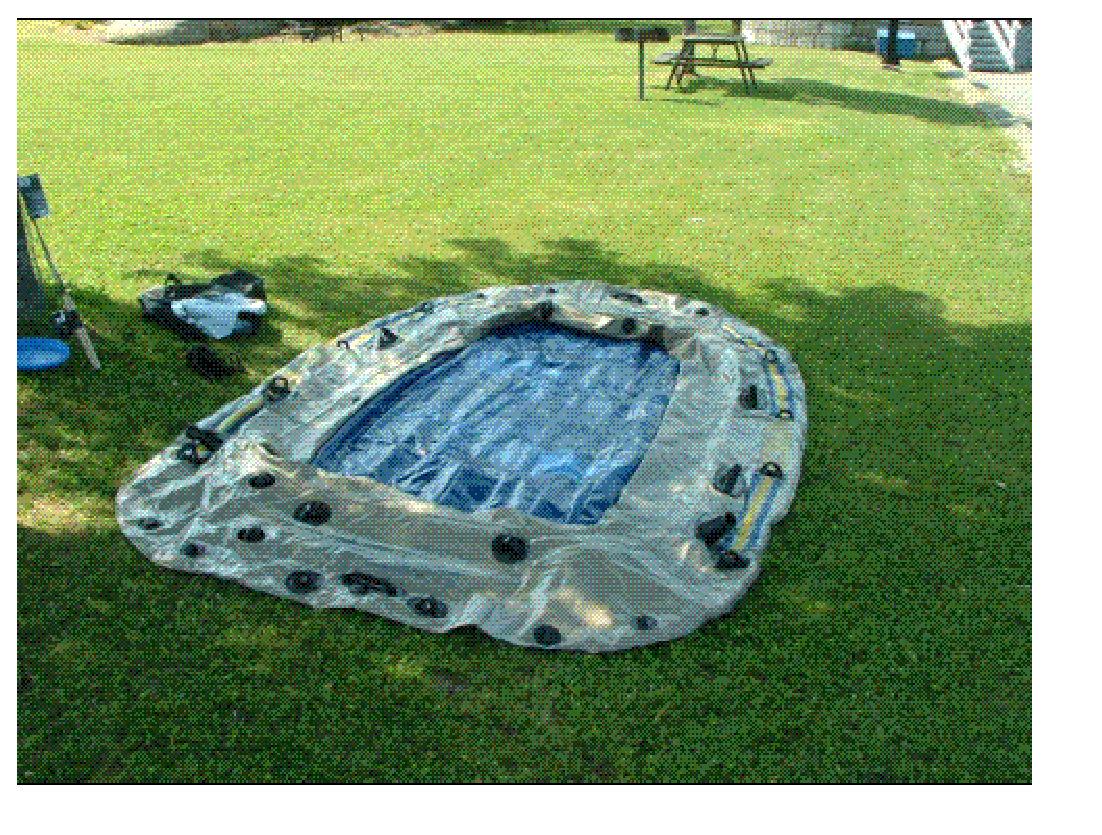
\epsfig{file=fig1.eps,width=3.5in}
Which one of the following is missing in it?
 
 
\noindent{\textbf{\large{
A.}}}
An air-boat
 
 
\noindent{\textbf{\large{
B.}}}
Lawn
 
 
\noindent{\textbf{\large{
C.}}}
A frisbee
 
 
\noindent{\textbf{\large{
D.}}}
A table
 
 
\noindent{\textbf{\large{
E.}}}
A truck
 
 
\noindent{\textbf{\large{
F.}}}
  Not any of aboves.
 
 
\noindent\vspace{0.05in}{\textbf{\Large{Auto-answer:}}}
 
 
\noindent{\textbf{\large{
E.}}}
A truck
 
 
\noindent\vspace{0.05in}{\textbf{\Large{End of auto-answer.}}}
 
 
 
\vspace{0.3in}
   
   
\noindent{\textbf{\Large{Total numbers: }}}
   
   
\noindent\begin{tabular}{|l|l|l|l|l|l|l|}
 \hline
Inputs & Calculates & Choices & Layers & Matches & Answer & Solution \\ \hline
           0  & 
           0  & 
           6
  simple  
  & 
           6  & 
           0  & 
  yes & 
  no 
  \\ \hline
 \end{tabular}
   
   
   
   
\noindent\vspace{0.1in}{\textbf{\Large{Calculated values:}}}
   
   
   
   
\noindent\vspace{0.1in}\hspace{-0.08in} {\textbf{\Large{All inputs: }}}
   
   
  
\vspace{0.2in}
  
{\textbf{\Large{Question
27.1.3 
 (           6 ,           7 ,          22 )
}}}
  
  
 
An object is subjected to an external net force $\mathbf{f}=(
30.0 ,
6.0,
-6000.0  )N$. Its mass is known as
$m= % 
56.0  kg$. Please choose the correct accelaration
from the following choices.
 
 
 
\noindent{\textbf{\large{
A.}}}
The accelaration (vector) is
$(
33534.,
1388.6 ,
4.0588 \times 10^{6}
)km/h^2.
$
 
 
\noindent{\textbf{\large{
B.}}}
The accelaration (vector) is
$(
33534.,
1388.6 ,
-1.3886 \times 10^{6}
)km/h^2.
$
 
 
\noindent{\textbf{\large{
C.}}}
The accelaration (vector) is
$(
31572.,
1388.6 ,
5.1924 \times 10^{6}
)km/h^2.
$
 
 
\noindent{\textbf{\large{
D.}}}
The accelaration (vector) is
$(
31572.,
1388.6 ,
4.0588 \times 10^{6}
)km/h^2.
$
 
 
\noindent{\textbf{\large{
E.}}}
The accelaration (vector) is
$(
33534.,
1388.6 ,
-4.2089 \times 10^{6}
)km/h^2.
$
 
 
\noindent{\textbf{\large{
F.}}}
The accelaration (vector) is
$(
32936.,
1388.6 ,
-1.3886 \times 10^{6}
)km/h^2.
$
 
 
\noindent{\textbf{\large{
G.}}}
The accelaration (vector) is
$(
32936.,
1388.6 ,
5.1924 \times 10^{6}
)km/h^2.
$
 
 
\noindent{\textbf{\large{
H.}}}
The accelaration (vector) is
$(
6942.9,
1388.6 ,
4.0588 \times 10^{6}
)km/h^2.
$
 
 
\noindent{\textbf{\large{
I.}}}
The accelaration (vector) is
$(
6942.9,
1388.6 ,
-4.2089 \times 10^{6}
)km/h^2.
$
 
 
\noindent{\textbf{\large{
J.}}}
The accelaration (vector) is
$(
33534.,
1388.6 ,
5.1924 \times 10^{6}
)km/h^2.
$
 
 
\noindent{\textbf{\large{
K.}}}
The accelaration (vector) is
$(
6942.9,
1388.6 ,
-1.3886 \times 10^{6}
)km/h^2.
$
 
 
\noindent{\textbf{\large{
L.}}}
The accelaration (vector) is
$(
32936.,
1388.6 ,
4.0588 \times 10^{6}
)km/h^2.
$
 
 
\noindent\vspace{0.05in}{\textbf{\Large{Auto-answer:}}}
 
 
\noindent{\textbf{\large{
K.}}}
The accelaration (vector) is
$(
6942.9,
1388.6 ,
-1.3886 \times 10^{6}
)km/h^2.
$
 
 
\noindent\vspace{0.05in}{\textbf{\Large{End of auto-answer.}}}
 
 
 
 
 
 
\noindent\vspace{0.1in}{\textbf{\Large{Solution: }}}
 
 

We will use the Newton's Second Law:
 
\[
\mathbf{f}=m\mathbf{a}.
\]
 
Since $\mathbf{f}=( % 
30.0,  % 
6.0,  % 
-6000.0 )N$
and $m= % 
56.0 kg$, bring them into the above equation, then we get
 
\begin{eqnarray*}
\mathbf{a}&=&\frac{\mathbf{f}}m  \\
&=&\frac{(
30.0 ,
6.0 ,
-6000.0 )N
}{ % 
56.0 kg}  \\
&=&(
0.53571 ,
0.10714,
-107.14
)ms^{-2} \\
&=&(
6942.9 ,
1388.6 ,
-1.3886 \times 10^{6}
)km/h^2.
\end{eqnarray*}
 
 
 
\noindent\vspace{0.1in}{\textbf{\Large{End of Solution.}}}
 
 

 
 
\vspace{0.3in}
   
   
\noindent{\textbf{\Large{Total numbers: }}}
   
   
\noindent\begin{tabular}{|l|l|l|l|l|l|l|}
 \hline
Inputs & Calculates & Choices & Layers & Matches & Answer & Solution \\ \hline
           4  & 
           6  & 
          12
  & 
           2  & 
           0  & 
  yes & 
  yes 
  \\ \hline
 \end{tabular}
   
   
   
   
\noindent\vspace{0.1in}{\textbf{\Large{Calculated values:}}}
   
   
  
  
\noindent\begin{tabular}{|l|l|l|l|}
\hline
 Sequential & Type & Accuracy & Calculated \\ 
\hline
 
 
  Calculated $            1 $ & real & $            5  $ & 
 $ 0.53571 $ 
 \\  \hline  
 
 
  Calculated $            2 $ & real & $            5  $ & 
 $ 0.10714 $ 
 \\  \hline  
 
 
  Calculated $            3 $ & real & $            5  $ & 
 $ -107.14 $ 
 \\  \hline  
 
 
  Calculated $            4 $ & real & $            5  $ & 
 $ 6942.9 $ 
 \\  \hline  
 
 
  Calculated $            5 $ & real & $            5  $ & 
 $ 1388.6 $ 
 \\  \hline  
 
 
  Calculated $            6 $ & real & $            5  $ & 
 $ -1.3886 \times 10^{6} $ 
 \\  \hline  
 \end{tabular}
   
   
   
   
\noindent\vspace{0.1in}\hspace{-0.08in} {\textbf{\Large{All inputs: }}}
   
   
  
  
\noindent\begin{tabular}{|l|l|l|l|l|}
\hline
 Sequential & Type & Accuracy & Three inputs & Generated \\ 
\hline
 
 
  INPUT $            1 $ & real & $           -1  $ & $
 20.0
  $ & \\
  & & &  $
 101.0
  $ & \\
  & & &  $
 10.0
 $ & $ 30.0 $ 
 \\  \hline  
 
 
  INPUT $            2 $ & real & $           -1  $ & $
 2.0
  $ & \\
  & & &  $
 10.1
  $ & \\
  & & &  $
 1.0
 $ & $ 6.0 $ 
 \\  \hline  
 
 
  INPUT $            3 $ & real & $           -1  $ & $
 -2000.0
  $ & \\
  & & &  $
 -10001.0
  $ & \\
  & & &  $
 -1000.0
 $ & $ -6000.0 $ 
 \\  \hline  
 \end{tabular}
   
   
  
  
\noindent\begin{tabular}{|l|l|l|l|l|}
\hline
 Sequential & Type & Accuracy & Three inputs & Generated \\ 
\hline
 
 
  INPUT $            4 $ & real & $           -1  $ & $
 50.0
  $ & \\
  & & &  $
 60.1
  $ & \\
  & & &  $
 2.0
 $ & $ 56.0 $ 
 \\  \hline  
 \end{tabular}
   
   
  
\vspace{0.2in}
  
{\textbf{\Large{Question
27.1.4 
 (           6 ,           8 ,          23 )
}}}
  
  
 
An object is subjected to an external net force $\mathbf{f}=(
20.0 ,
6.0,
-3000.0  )N$. Its mass is known as
$m= % 
52.0  kg$. Please choose the correct accelaration
from the following choices.
 
 
 
\noindent{\textbf{\large{
A.}}}
The accelaration is
$(
-1.3940ms^{-2},
0.11538ms^{-2},
1.7163 \times 10^{6}km/h^2
).
$
 
 
\noindent{\textbf{\large{
B.}}}
The accelaration is
$(
-1.3940ms^{-2},
0.50998ms^{-2},
1.7163 \times 10^{6}km/h^2
).
$
 
 
\noindent{\textbf{\large{
C.}}}
The accelaration is
$(
0.38462ms^{-2},
0.11538ms^{-2},
-747692.km/h^2
).
$
 
 
\noindent{\textbf{\large{
D.}}}
The accelaration is
$(
0.38462ms^{-2},
0.50998ms^{-2},
1.7163 \times 10^{6}km/h^2
).
$
 
 
\noindent{\textbf{\large{
E.}}}
none of these.
 
 
\noindent\vspace{0.05in}{\textbf{\Large{Auto-answer:}}}
 
 
\noindent{\textbf{\large{
C.}}}
The accelaration is
$(
0.38462ms^{-2},
0.11538ms^{-2},
-747692.km/h^2
).
$
 
 
\noindent\vspace{0.05in}{\textbf{\Large{End of auto-answer.}}}
 
 
 
 
 
 
\noindent\vspace{0.1in}{\textbf{\Large{Solution: }}}
 
 

We will use the Newton's Second Law:
 
\[
\mathbf{f}=m\mathbf{a}.
\]
 
Since $\mathbf{f}=( % 
20.0,  % 
6.0,  % 
-3000.0 )N$
and $m= % 
52.0kg$, bring them into the above equation, then we get
 
\begin{eqnarray*}
\mathbf{a}&=&\frac{\mathbf{f}}m  \\
&=&\frac{(
20.0 ,
6.0 ,
-3000.0 )N
}{ % 
52.0 kg}  \\
&=&(
0.38462 ,
0.11538,
-57.692
)ms^{-2} \\
&=&(
4984.6 ,
1495.4 ,
-747692.
)km/h^2.
\end{eqnarray*}
 
 
 
\noindent\vspace{0.1in}{\textbf{\Large{End of Solution.}}}
 
 

 
\vspace{0.3in}
   
   
\noindent{\textbf{\Large{Total numbers: }}}
   
   
\noindent\begin{tabular}{|l|l|l|l|l|l|l|}
 \hline
Inputs & Calculates & Choices & Layers & Matches & Answer & Solution \\ \hline
           4  & 
           6  & 
           5
  & 
           3  & 
           0  & 
  yes & 
  yes 
  \\ \hline
 \end{tabular}
   
   
   
   
\noindent\vspace{0.1in}{\textbf{\Large{Calculated values:}}}
   
   
  
  
\noindent\begin{tabular}{|l|l|l|l|}
\hline
 Sequential & Type & Accuracy & Calculated \\ 
\hline
 
 
  Calculated $            1 $ & real & $            5  $ & 
 $ 0.38462 $ 
 \\  \hline  
 
 
  Calculated $            2 $ & real & $            5  $ & 
 $ 0.11538 $ 
 \\  \hline  
 
 
  Calculated $            3 $ & real & $            5  $ & 
 $ -57.692 $ 
 \\  \hline  
 
 
  Calculated $            4 $ & real & $            5  $ & 
 $ 4984.6 $ 
 \\  \hline  
 
 
  Calculated $            5 $ & real & $            5  $ & 
 $ 1495.4 $ 
 \\  \hline  
 
 
  Calculated $            6 $ & real & $            5  $ & 
 $ -747692. $ 
 \\  \hline  
 \end{tabular}
   
   
   
   
\noindent\vspace{0.1in}\hspace{-0.08in} {\textbf{\Large{All inputs: }}}
   
   
  
  
\noindent\begin{tabular}{|l|l|l|l|l|}
\hline
 Sequential & Type & Accuracy & Three inputs & Generated \\ 
\hline
 
 
  INPUT $            1 $ & real & $           -1  $ & $
 20.0
  $ & \\
  & & &  $
 101.0
  $ & \\
  & & &  $
 10.0
 $ & $ 20.0 $ 
 \\  \hline  
 
 
  INPUT $            2 $ & real & $           -1  $ & $
 2.0
  $ & \\
  & & &  $
 10.1
  $ & \\
  & & &  $
 1.0
 $ & $ 6.0 $ 
 \\  \hline  
 
 
  INPUT $            3 $ & real & $           -1  $ & $
 -2000.0
  $ & \\
  & & &  $
 -10001.0
  $ & \\
  & & &  $
 -1000.0
 $ & $ -3000.0 $ 
 \\  \hline  
 \end{tabular}
   
   
  
  
\noindent\begin{tabular}{|l|l|l|l|l|}
\hline
 Sequential & Type & Accuracy & Three inputs & Generated \\ 
\hline
 
 
  INPUT $            4 $ & real & $           -1  $ & $
 50.0
  $ & \\
  & & &  $
 60.1
  $ & \\
  & & &  $
 2.0
 $ & $ 52.0 $ 
 \\  \hline  
 \end{tabular}
   
   
  
\vspace{0.2in}
  
{\textbf{\Large{Question
27.1.5 
 (           6 ,          13 ,          28 )
}}}
  
  
What is the operation between $a= % 
7$ and $b= % 
6$:
$a$  % 
$\times$ $b=?$ Please also calculate it.
 
 
\noindent\vspace{0.05in}{\textbf{\Large{Answer:}}}
 
 

7;
 
6;
 
The operation is  % 
MULTIPLICATION and the result is
$ % 
42.000$.
 
 
 
\noindent\vspace{0.05in}{\textbf{\Large{End of Answer.}}}
 
 

 
\vspace{0.3in}
   
   
\noindent{\textbf{\Large{Total numbers: }}}
   
   
\noindent\begin{tabular}{|l|l|l|l|l|l|l|}
 \hline
Inputs & Calculates & Choices & Layers & Matches & Answer & Solution \\ \hline
           3  & 
           2  & 
           0
  & 
           0  & 
           0  & 
  yes & 
  no 
  \\ \hline
 \end{tabular}
   
   
   
   
\noindent\vspace{0.1in}{\textbf{\Large{Calculated values:}}}
   
   
  
  
\noindent\begin{tabular}{|l|l|l|l|}
\hline
 Sequential & Type & Accuracy & Calculated \\ 
\hline
 
 
  Calculated $            1 $ & string & $            1  $ ( $           1  $ strings): 
 & MULTIPLICATION
 \\  \hline  
 
 
  Calculated $            2 $ & real & $            5  $ & 
 $ 42.000 $ 
 \\  \hline  
 \end{tabular}
   
   
   
   
\noindent\vspace{0.1in}\hspace{-0.08in} {\textbf{\Large{All inputs: }}}
   
   
  
  
\noindent\begin{tabular}{|l|l|l|l|l|}
\hline
 Sequential & Type & Accuracy & Three inputs & Generated \\ 
\hline
 
 
  INPUT $            1 $ & integer &  & $
 1
 , 
 10
 , 
 2
 $ & $ 7 $ 
 \\  \hline  
 
 
  INPUT $            2 $ & integer &  & $
 2
 , 
 10
 , 
 2
 $ & $ 6 $ 
 \\  \hline  
 
 
  INPUT $            3 $ & string & & 
 $+$ & 
  \\
  & & & 
 $-$ & 
  \\
  & & & 
 $\times$ & 
  $ <-- $ 
  \\
  & & & 
 $\div$ & 
 \\  \hline  
 \end{tabular}
   
   
  
\vspace{0.2in}
  
{\textbf{\Large{Question
27.1.6 
 (           6 ,          11 ,          26 )
}}}
  
  
In a hotel, the possiblity of  % 
non-smoking customer is
$a =  % 
7.0 \times 10^{-2}$, and the possiblity of  % 
equal or above 30 years old customer is $ b =  % 
0.6800$.
Please calculate the possiblity of  % 
smoking and  % 
under 30 years old customer.
 
 
 
\noindent\vspace{0.1in}{\textbf{\Large{Solution: }}}
 
 

Since the possiblity of  % 
 non-smoking customer is $ a =  % 
7.0 \times 10^{-2} $,
and the possiblity of  % 
equal or above 30 years old customer is $ b =  % 
0.6800 $,
the possiblity of  % 
smoking customer is $ c = 1.0 - a = 1.0 -
7.0 \times 10^{-2}
=  % 
0.930 $ and the possiblity of  % 
under 30 years old
customer is $ d = 1.0 - b = 1.0 -  % 
0.6800 =  % 
0.3200  $.
So the possibility of  % 
smoking and  % 
under 30 years old
customer is $ c \times d =  % 
0.298 $.
 
 
 
\noindent\vspace{0.1in}{\textbf{\Large{End of Solution.}}}
 
 

 
 
 
\noindent\vspace{0.05in}{\textbf{\Large{Answer:}}}
 
 

The possibility of  % 
smoking and  % 
under 30 years old
customer is $ (1-a)(1-b) =  % 
0.298 $.
 
 
\noindent\vspace{0.05in}{\textbf{\Large{End of Answer.}}}
 
 

 
\vspace{0.3in}
   
   
\noindent{\textbf{\Large{Total numbers: }}}
   
   
\noindent\begin{tabular}{|l|l|l|l|l|l|l|}
 \hline
Inputs & Calculates & Choices & Layers & Matches & Answer & Solution \\ \hline
           4  & 
           3  & 
           0
  & 
           0  & 
           0  & 
  yes & 
  yes 
  \\ \hline
 \end{tabular}
   
   
   
   
\noindent\vspace{0.1in}{\textbf{\Large{Calculated values:}}}
   
   
  
  
\noindent\begin{tabular}{|l|l|l|l|}
\hline
 Sequential & Type & Accuracy & Calculated \\ 
\hline
 
 
  Calculated $            1 $ & real & $            3  $ & 
 $ 0.930 $ 
 \\  \hline  
 
 
  Calculated $            2 $ & real & $            4  $ & 
 $ 0.3200 $ 
 \\  \hline  
 
 
  Calculated $            3 $ & real & $            3  $ & 
 $ 0.298 $ 
 \\  \hline  
 \end{tabular}
   
   
   
   
\noindent\vspace{0.1in}\hspace{-0.08in} {\textbf{\Large{All inputs: }}}
   
   
  
  
\noindent\begin{tabular}{|l|l|l|l|l|}
\hline
 Sequential & Type & Accuracy & Three inputs & Generated \\ 
\hline
 
 
  INPUT $            1 $ & logical & .TRUE. & 
 smoking & 
  \\
  & & .FALSE. & 
  non-smoking & 
  $ <-- $ 
 \\  \hline  
 
 
  INPUT $            2 $ & real & $           -3  $ & $
 1.0 \times 10^{-2}
  $ & \\
  & & &  $
 1.000
  $ & \\
  & & &  $
 1.0 \times 10^{-2}
 $ & $ 7.0 \times 10^{-2} $ 
 \\  \hline  
 
 
  INPUT $            3 $ & logical & .TRUE. & 
 equal or above 30 years old & 
  $ <-- $ 
  \\
  & & .FALSE. & 
  under 30 years old & 
 \\  \hline  
 \end{tabular}
   
   
  
  
\noindent\begin{tabular}{|l|l|l|l|l|}
\hline
 Sequential & Type & Accuracy & Three inputs & Generated \\ 
\hline
 
 
  INPUT $            4 $ & real & $           -4  $ & $
 2.00 \times 10^{-2}
  $ & \\
  & & &  $
 1.0000
  $ & \\
  & & &  $
 2.00 \times 10^{-2}
 $ & $ 0.6800 $ 
 \\  \hline  
 \end{tabular}
   
   
   
   
\vspace{0.3in}
{\textbf{\LARGE{You have done all the above? A very good beginning, please go ahead.}}}
More constants the
Mass of electron
$m_e$$ =
9.109390 \times 10^{-31} $
kg
,
Universal gas constant
$R$$ =
8.315 $
J/(mol$\cdot $K)
,
$e$$ =
1.60217733 \times 10^{-19} $
C
, and
$m_p$$ =
1.6726231 \times 10^{-27} $
kg
%
may be very helpful.
\vspace{0.3in}
   
   
  
\vspace{0.2in}
  
{\textbf{\Large{QUESTION
27.2 
 (           1 ,           1 ,           1 )
}}}
  
  


\noindent\vspace{0.05in}{\textbf{\Large{Abstract:}}}
This is a simple Newton's Second Law calculation multi-choice problem.  
\noindent\vspace{0.05in}{\textbf{\Large{end of abstract.}}}


 
 
An object is subjected to an external net force $\mathbf{f}=
(40.0 , 9.0 , -7000.0) N$.
Its mass is known as $m= % 
58.0000 kg$. Please choose the
correct accelaration from the following choices.
 
 
 
\noindent{\textbf{\large{
A.}}}
The accelaration is $  %
(
0.690,
0.16,
-120.69)
ms^{-2} $.
 
 
\noindent{\textbf{\large{
B.}}}
The accelaration is $  %
(
-2.04,
0.46,
576.39)
ms^{-2} $.
 
 
\noindent{\textbf{\large{
C.}}}
The accelaration is $  %
(
-2.04,
0.46,
-120.69)
ms^{-2} $.
 
 
\noindent{\textbf{\large{
D.}}}
The accelaration is $  %
(
0.690,
0.46,
-120.69)
ms^{-2} $.
 
 
\noindent{\textbf{\large{
E.}}}
The accelaration is $  %
(
-2.04,
0.16,
-120.69)
ms^{-2} $.
 
 
\noindent{\textbf{\large{
F.}}}
The accelaration is $  %
(
0.690,
0.46,
576.39)
ms^{-2} $.
 
 
\noindent{\textbf{\large{
G.}}}
The accelaration is $  %
(
0.690,
0.16,
576.39)
ms^{-2} $.
 
 
\noindent{\textbf{\large{
H.}}}
The accelaration is $  %
(
-2.04,
0.16,
576.39)
ms^{-2} $.
 
 
\noindent\vspace{0.05in}{\textbf{\Large{Auto-answer:}}}
 
 
\noindent{\textbf{\large{
A.}}}
The accelaration is $  %
(
0.690,
0.16,
-120.69)
ms^{-2} $.
 
 
\noindent\vspace{0.05in}{\textbf{\Large{End of auto-answer.}}}
 
 
 
 
 
\noindent\vspace{0.05in}{\textbf{\Large{Answer:}}}
 
 

The correct answer from the choices is


\noindent{\textbf{\large{
A.}}}
The accelaration is $  %
(
0.690,
0.16,
-120.69)
ms^{-2} $.
 
 
 
\noindent\vspace{0.05in}{\textbf{\Large{End of Answer.}}}
 
 

 
 
 
\noindent\vspace{0.1in}{\textbf{\Large{Solution: }}}
 
 

We will use the Newton's Second Law:
 
\[
\mathbf{f}=m\mathbf{a}.
\]
 
Since $\mathbf{f}= % 
(40.0 , 9.0 , -7000.0) N$
and $m= % 
58.0000kg$, bring them into the above equation, then we get
 
\begin{eqnarray*}
\mathbf{a}&=&\frac{\mathbf{f}}m  \\
&=&\frac{ % 
(40.0 , 9.0 , -7000.0) N}{ % 
58.0000kg}  \\
&=& % 
(0.690 , 0.16 , -120.69) ms^{-2}
\end{eqnarray*}
 
 
 
\noindent\vspace{0.1in}{\textbf{\Large{End of Solution.}}}
 
 

 
\vspace{0.3in}
   
   
\noindent{\textbf{\Large{Total numbers: }}}
   
   
\noindent\begin{tabular}{|l|l|l|l|l|l|l|}
 \hline
Inputs & Calculates & Choices & Layers & Matches & Answer & Solution \\ \hline
           2  & 
           1  & 
           8
  & 
           3  & 
           0  & 
  yes & 
  yes 
  \\ \hline
 \end{tabular}
   
   
   
   
\noindent\vspace{0.1in}{\textbf{\Large{Calculated values:}}}
   
   
  
  
\noindent\begin{tabular}{|l|l|l|l|}
\hline
 Sequential & Type & Accuracy & Calculated \\ 
\hline
 
 
  Calculated $            1 $ & vector &  
  $            3  $ 
 &  $ 0.690 $ 
 \\    
  & & 
  $            2  $ 
 &  $ 0.16 $ 
 \\    
  & & 
  $            5  $ 
 &  $ -120.69 $ 
 \\  \hline  
 \end{tabular}
   
   
   
   
\noindent\vspace{0.1in}\hspace{-0.08in} {\textbf{\Large{All inputs: }}}
   
   
  
  
\noindent\begin{tabular}{|l|l|l|l|l|}
\hline
 Sequential & Type & Accuracy & Three inputs & Generated \\ 
\hline
 
 
  INPUT $            1 $ & vector & $           -1  $ & $
20.0
  $ & \\
  & & & $
101.0
  $ & \\
  & & & $
10.0
$ & $ 40.0 $ 
  \\
  & & $           -1  $ & $
2.0
  $ & \\
  & & & $
10.1
  $ & \\
  & & & $
1.0
$ & $ 9.0 $ 
  \\
  & & $           -1  $ & $
-2000.0
  $ & \\
  & & & $
-10001.0
  $ & \\
  & & & $
-1000.0
$ & $ -7000.0 $ 
 \\  \hline  
 
 
  INPUT $            2 $ & real & $           -4  $ & $
 50.0000
  $ & \\
  & & &  $
 60.1000
  $ & \\
  & & &  $
 2.0000
 $ & $ 58.0000 $ 
 \\  \hline  
 \end{tabular}
   
   
  
\vspace{0.2in}
  
{\textbf{\Large{QUESTION
27.3 
 (           3 ,           3 ,           3 )
}}}
  
  
Please choose the correct one from the following statements:
 
 
\noindent{\textbf{\large{
A.}}}
Canada has  %
35 provinces and  %
34 territories.
 
 
\noindent{\textbf{\large{
B.}}}
Canada has  %
37 provinces and  %
37 territories.
 
 
\noindent{\textbf{\large{
C.}}}
Canada has  %
34 provinces and  %
39 territories.
 
 
\noindent{\textbf{\large{
D.}}}
Canada has  %
33 provinces and  %
38 territories.
 
 
\noindent{\textbf{\large{
E.}}}
Canada has  %
10 provinces and  %
3 territories.
 
 
\noindent{\textbf{\large{
F.}}}
 None of above.
 
 
\noindent\vspace{0.05in}{\textbf{\Large{Auto-answer:}}}
 
 
\noindent{\textbf{\large{
E.}}}
Canada has  %
10 provinces and  %
3 territories.
 
 
\noindent\vspace{0.05in}{\textbf{\Large{End of auto-answer.}}}
 
 
   
   
\noindent{\textbf{\Large{Total numbers: }}}
   
   
\noindent\begin{tabular}{|l|l|l|l|l|l|l|}
 \hline
Inputs & Calculates & Choices & Layers & Matches & Answer & Solution \\ \hline
           0  & 
          20  & 
           6
  simple  
  & 
           6  & 
           0  & 
  yes & 
  no 
  \\ \hline
 \end{tabular}
   
   
   
   
\noindent\vspace{0.1in}{\textbf{\Large{Calculated values:}}}
   
   
  
  
\noindent\begin{tabular}{|l|l|l|l|}
\hline
 Sequential & Type & Accuracy & Calculated \\ 
\hline
 
 
  Calculated $            1 $ & integer &  & 
  $ 10 $ 
 \\  \hline  
 
 
  Calculated $            2 $ & integer &  & 
  $ 3 $ 
 \\  \hline  
 
 
  Calculated $            3 $ & integer &  & 
  $ 23 $ 
 \\  \hline  
 
 
  Calculated $            4 $ & integer &  & 
  $ 24 $ 
 \\  \hline  
 
 
  Calculated $            5 $ & integer &  & 
  $ 25 $ 
 \\  \hline  
 
 
  Calculated $            6 $ & integer &  & 
  $ 26 $ 
 \\  \hline  
 
 
  Calculated $            7 $ & integer &  & 
  $ 27 $ 
 \\  \hline  
 
 
  Calculated $            8 $ & integer &  & 
  $ 28 $ 
 \\  \hline  
 
 
  Calculated $            9 $ & integer &  & 
  $ 29 $ 
 \\  \hline  
 
 
  Calculated $           10 $ & integer &  & 
  $ 30 $ 
 \\  \hline  
 \end{tabular}
   
   
  
  
\noindent\begin{tabular}{|l|l|l|l|}
\hline
 Sequential & Type & Accuracy & Calculated \\ 
\hline
 
 
  Calculated $           11 $ & integer &  & 
  $ 31 $ 
 \\  \hline  
 
 
  Calculated $           12 $ & integer &  & 
  $ 32 $ 
 \\  \hline  
 
 
  Calculated $           13 $ & integer &  & 
  $ 33 $ 
 \\  \hline  
 
 
  Calculated $           14 $ & integer &  & 
  $ 34 $ 
 \\  \hline  
 
 
  Calculated $           15 $ & integer &  & 
  $ 35 $ 
 \\  \hline  
 
 
  Calculated $           16 $ & integer &  & 
  $ 36 $ 
 \\  \hline  
 
 
  Calculated $           17 $ & integer &  & 
  $ 37 $ 
 \\  \hline  
 
 
  Calculated $           18 $ & integer &  & 
  $ 38 $ 
 \\  \hline  
 
 
  Calculated $           19 $ & integer &  & 
  $ 39 $ 
 \\  \hline  
 
 
  Calculated $           20 $ & integer &  & 
  $ 40 $ 
 \\  \hline  
 \end{tabular}
   
   
   
   
\noindent\vspace{0.1in}\hspace{-0.08in} {\textbf{\Large{All inputs: }}}
   
   
  
\vspace{0.2in}
  
{\textbf{\Large{QUESTION
27.4 
 (           2 ,           2 ,           2 )
}}}
  
  
 
An object is subjected to an external net force $\mathbf{f}=(
40.000 ,
3.0000,
-3000.0  )N$. Its mass is known as
$m= % 
54.0000  kg$. Please choose the correct accelaration
from the following choices.
 
 
 
\noindent{\textbf{\large{
A.}}}
The accelaration is
$(
0.74074ms^{-2},
720.00km/h^2,
-55.556ms^{-2}
).
$
 
 
\noindent{\textbf{\large{
B.}}}
The accelaration is
$(
3.0767ms^{-2},
720.00km/h^2,
237.05ms^{-2}
).
$
 
 
\noindent{\textbf{\large{
C.}}}
The accelaration is
$(
3.0767ms^{-2},
3596.1km/h^2,
-55.556ms^{-2}
).
$
 
 
\noindent{\textbf{\large{
D.}}}
The accelaration is
$(
0.74074ms^{-2},
3596.1km/h^2,
237.05ms^{-2}
).
$
 
 
\noindent{\textbf{\large{
E.}}}
The accelaration is
$(
0.74074ms^{-2},
3596.1km/h^2,
-55.556ms^{-2}
).
$
 
 
\noindent{\textbf{\large{
F.}}}
The accelaration is
$(
3.0767ms^{-2},
720.00km/h^2,
-55.556ms^{-2}
).
$
 
 
\noindent{\textbf{\large{
G.}}}
 None of these.
 
 
\noindent\vspace{0.05in}{\textbf{\Large{Auto-answer:}}}
 
 
\noindent{\textbf{\large{
A.}}}
The accelaration is
$(
0.74074ms^{-2},
720.00km/h^2,
-55.556ms^{-2}
).
$
 
 
\noindent\vspace{0.05in}{\textbf{\Large{End of auto-answer.}}}
 
 
 
 
 
 
\noindent\vspace{0.1in}{\textbf{\Large{Solution: }}}
 
 

We will use the Newton's Second Law:
 
\[
\mathbf{f}=m\mathbf{a}.
\]
 
Since $\mathbf{f}=( % 
40.000,  % 
3.0000,  % 
-3000.0 )N$
and $m= % 
54.0000kg$, bring them into the above equation, then we get
 
\begin{eqnarray*}
\mathbf{a}&=&\frac{\mathbf{f}}m  \\
&=&\frac{(
40.000 ,
3.0000 ,
-3000.0 )N
}{ % 
54.0000 kg}  \\
&=&(
0.74074 ,
5.5556 \times 10^{-2},
-55.556
)ms^{-2} \\
&=&(
9600.0 ,
720.00 ,
-720000.
)km/h^2.
\end{eqnarray*}
 
 
 
\noindent\vspace{0.1in}{\textbf{\Large{End of Solution.}}}
 
 

 
\vspace{0.3in}
   
   
\noindent{\textbf{\Large{Total numbers: }}}
   
   
\noindent\begin{tabular}{|l|l|l|l|l|l|l|}
 \hline
Inputs & Calculates & Choices & Layers & Matches & Answer & Solution \\ \hline
           4  & 
           6  & 
           7
  & 
           3  & 
           0  & 
  yes & 
  yes 
  \\ \hline
 \end{tabular}
   
   
   
   
\noindent\vspace{0.1in}{\textbf{\Large{Calculated values:}}}
   
   
  
  
\noindent\begin{tabular}{|l|l|l|l|}
\hline
 Sequential & Type & Accuracy & Calculated \\ 
\hline
 
 
  Calculated $            1 $ & real & $            5  $ & 
 $ 0.74074 $ 
 \\  \hline  
 
 
  Calculated $            2 $ & real & $            5  $ & 
 $ 5.5556 \times 10^{-2} $ 
 \\  \hline  
 
 
  Calculated $            3 $ & real & $            5  $ & 
 $ -55.556 $ 
 \\  \hline  
 
 
  Calculated $            4 $ & real & $            5  $ & 
 $ 9600.0 $ 
 \\  \hline  
 
 
  Calculated $            5 $ & real & $            5  $ & 
 $ 720.00 $ 
 \\  \hline  
 
 
  Calculated $            6 $ & real & $            5  $ & 
 $ -720000. $ 
 \\  \hline  
 \end{tabular}
   
   
   
   
\noindent\vspace{0.1in}\hspace{-0.08in} {\textbf{\Large{All inputs: }}}
   
   
  
  
\noindent\begin{tabular}{|l|l|l|l|l|}
\hline
 Sequential & Type & Accuracy & Three inputs & Generated \\ 
\hline
 
 
  INPUT $            1 $ & real & $           -3  $ & $
 20.000
  $ & \\
  & & &  $
 101.000
  $ & \\
  & & &  $
 10.000
 $ & $ 40.000 $ 
 \\  \hline  
 
 
  INPUT $            2 $ & real & $           -4  $ & $
 2.0000
  $ & \\
  & & &  $
 10.1000
  $ & \\
  & & &  $
 1.0000
 $ & $ 3.0000 $ 
 \\  \hline  
 
 
  INPUT $            3 $ & real & $           -1  $ & $
 -2000.0
  $ & \\
  & & &  $
 -10001.0
  $ & \\
  & & &  $
 -1000.0
 $ & $ -3000.0 $ 
 \\  \hline  
 \end{tabular}
   
   
  
  
\noindent\begin{tabular}{|l|l|l|l|l|}
\hline
 Sequential & Type & Accuracy & Three inputs & Generated \\ 
\hline
 
 
  INPUT $            4 $ & real & $           -4  $ & $
 50.0000
  $ & \\
  & & &  $
 60.1000
  $ & \\
  & & &  $
 2.0000
 $ & $ 54.0000 $ 
 \\  \hline  
 \end{tabular}
   
   
  
\vspace{0.2in}
  
{\textbf{\Large{QUESTION
27.5 
 (           4 ,           4 ,           4 )
}}}
  
  
Considering case-insensitivity, please match the following same strings.
  
  
\begin{tabular}{|l|l|l|}
 \hline
 Column Left & Column Right  & Your choinces \\ 
 \hline
{\textbf{\large{
A.}}}
C
  & 
eR
 & 
 \\ 
 \hline
{\textbf{\large{
B.}}}
 A= %
2/ %
2

  & 
 a= %
1
 & 
 \\ 
 \hline
{\textbf{\large{
C.}}}
yjh
  & 
ER
 & 
 \\ 
 \hline
{\textbf{\large{
D.}}}
Er
  & 
YJH
 & 
 \\ 
 \hline
{\textbf{\large{
E.}}}
er
  & 
c
 & 
 \\ 
 \hline
 \end{tabular}
  
  
 
 
\noindent\vspace{0.05in}{\textbf{\Large{Auto-answer:}}}
  
  
\begin{tabular}{|l|l|l|}
 \hline
 Column Left & Column Right  & Answers       \\ 
 \hline
{\textbf{\large{
A.}}}
C
  & 
eR
 & 
{\textbf{\large{
D.}}}
, 
{\textbf{\large{
E.}}}
 \\ 
 \hline
{\textbf{\large{
B.}}}
 A= %
2/ %
2

  & 
 a= %
1
 & 
{\textbf{\large{
B.}}}
 \\ 
 \hline
{\textbf{\large{
C.}}}
yjh
  & 
ER
 & 
{\textbf{\large{
D.}}}
, 
{\textbf{\large{
E.}}}
 \\ 
 \hline
{\textbf{\large{
D.}}}
Er
  & 
YJH
 & 
{\textbf{\large{
C.}}}
 \\ 
 \hline
{\textbf{\large{
E.}}}
er
  & 
c
 & 
{\textbf{\large{
A.}}}
 \\ 
 \hline
 \end{tabular}
  
  
 
 
\noindent\vspace{0.05in}{\textbf{\Large{End of auto-answer.}}}
 
 
 
   
   
\noindent{\textbf{\Large{Total numbers: }}}
   
   
\noindent\begin{tabular}{|l|l|l|l|l|l|l|}
 \hline
Inputs & Calculates & Choices & Layers & Matches & Answer & Solution \\ \hline
           2  & 
           1  & 
           0
  & 
          16  & 
           5  & 
  yes & 
  no 
  \\ \hline
 \end{tabular}
   
   
   
   
\noindent\vspace{0.1in}{\textbf{\Large{Calculated values:}}}
   
   
  
  
\noindent\begin{tabular}{|l|l|l|l|}
\hline
 Sequential & Type & Accuracy & Calculated \\ 
\hline
 
 
  Calculated $            1 $ & integer &  & 
  $ 1 $ 
 \\  \hline  
 \end{tabular}
   
   
   
   
\noindent\vspace{0.1in}\hspace{-0.08in} {\textbf{\Large{All inputs: }}}
   
   
  
  
\noindent\begin{tabular}{|l|l|l|l|l|}
\hline
 Sequential & Type & Accuracy & Three inputs & Generated \\ 
\hline
 
 
  INPUT $            1 $ & integer &  & $
 2
 , 
 8
 , 
 2
 $ & $ 2 $ 
 \\  \hline  
 
 
  INPUT $            2 $ & integer &  & $
 2
 , 
 3
 , 
 2
 $ & $ 2 $ 
 \\  \hline  
 \end{tabular}
   
   
  
\vspace{0.2in}
  
{\textbf{\Large{QUESTION
27.6 
 (           5 ,           5 ,           5 )
}}}
  
  
If any one of the following statements is correct, please fill the box ahead of it with $T$ .
If wrong, fill with $F$.
 
\noindent\begin{tabular}{|l|l|}\hline Your&\hspace{.2in} \\ answer&\hspace{.2in} \\ \hline \end{tabular}
1. $ % 
22$ is an  % 
odd number.
 
\noindent\begin{tabular}{|l|l|}\hline Your&\hspace{.2in} \\ answer&\hspace{.2in} \\ \hline \end{tabular}
2.  % 
Toronto is in  % 
Ontario province.
 
\noindent\begin{tabular}{|l|l|}\hline Your&\hspace{.2in} \\ answer&\hspace{.2in} \\ \hline \end{tabular}
3.  % 
$\mathbf{F}=m\mathbf{a}$ is a mathmatical form of
the Newton's Second Law.
 
 
 
\noindent\vspace{0.05in}{\textbf{\Large{Answer:}}}
 
 

 
\noindent\begin{tabular}{|l|l|}\hline The correct & \\
          answer &  % 
$F$ \\ \hline \end{tabular}
1. $ % 
22$ is an  % 
odd number.
 
\noindent\begin{tabular}{|l|l|}\hline The correct & \\
          answer &  % 
$T$ \\ \hline \end{tabular}
2.  % 
Toronto is in  % 
Ontario province.
 
\noindent\begin{tabular}{|l|l|}\hline The correct & \\
          answer &  % 
$T$ \\ \hline \end{tabular}
3.  % 
$\mathbf{F}=m\mathbf{a}$ is a mathmatical form of  % 
the Newton's Second Law.
 
 
 
\noindent\vspace{0.05in}{\textbf{\Large{End of Answer.}}}
 
 

 
\vspace{0.3in}
   
   
\noindent{\textbf{\Large{Total numbers: }}}
   
   
\noindent\begin{tabular}{|l|l|l|l|l|l|l|}
 \hline
Inputs & Calculates & Choices & Layers & Matches & Answer & Solution \\ \hline
           6  & 
           3  & 
           0
  & 
           0  & 
           0  & 
  yes & 
  no 
  \\ \hline
 \end{tabular}
   
   
   
   
\noindent\vspace{0.1in}{\textbf{\Large{Calculated values:}}}
   
   
  
  
\noindent\begin{tabular}{|l|l|l|l|}
\hline
 Sequential & Type & Accuracy & Calculated \\ 
\hline
 
 
  Calculated $            1 $ & string & $            1  $ ( $           1  $ strings): 
 & $F$
 \\  \hline  
 
 
  Calculated $            2 $ & string & $            1  $ ( $           1  $ strings): 
 & $T$
 \\  \hline  
 
 
  Calculated $            3 $ & string & $            1  $ ( $           1  $ strings): 
 & $T$
 \\  \hline  
 \end{tabular}
   
   
   
   
\noindent\vspace{0.1in}\hspace{-0.08in} {\textbf{\Large{All inputs: }}}
   
   
  
  
\noindent\begin{tabular}{|l|l|l|l|l|}
\hline
 Sequential & Type & Accuracy & Three inputs & Generated \\ 
\hline
 
 
  INPUT $            1 $ & integer &  & $
 1
 , 
 100
 , 
 1
 $ & $ 22 $ 
 \\  \hline  
 
 
  INPUT $            2 $ & string & & 
 even & 
  \\
  & & & 
 odd & 
  $ <-- $ 
 \\  \hline  
 
 
  INPUT $            3 $ & string & & 
 Toronto & 
  $ <-- $ 
  \\
  & & & 
 Kingston & 
  \\
  & & & 
 Montreal & 
  \\
  & & & 
 Hull & 
 \\  \hline  
 \end{tabular}
   
   
  
  
\noindent\begin{tabular}{|l|l|l|l|l|}
\hline
 Sequential & Type & Accuracy & Three inputs & Generated \\ 
\hline
 
 
  INPUT $            4 $ & string & & 
 Ontario & 
  $ <-- $ 
  \\
  & & & 
 Quebec & 
 \\  \hline  
 
 
  INPUT $            5 $ & string & & 
 $\mathbf{F}=m\mathbf{a}$ & 
  $ <-- $ 
  \\
  & & & 
 $\left| \mathbf{F}\right| =Gm_1m_2r^{-2}$ & 
 \\  \hline  
 
 
  INPUT $            6 $ & string & & 
 the Newton's Second Law & 
  $ <-- $ 
  \\
  & & & 
 Newton's Law of Universal Gravitation & 
 \\  \hline  
 \end{tabular}
   
   
   
   
\vspace{0.3in}
{\textbf{\LARGE{You have done all the above? Excellent! Not much left, please continue.}}}
\vspace{0.3in}
   
   
  
\vspace{0.2in}
  
{\textbf{\Large{QUESTION
27.7 
 (           8 ,          15 ,          60 )
}}}
  
  
 
$ \left( \begin{array}{ccccccccc}
           5  & 
           4  & 
           5  & 
           4  \\ 
           5  & 
           6  & 
           5  & 
           6  \\ 
           5  & 
           6  & 
           6  & 
           5
\end{array}\right) \times
\left( \begin{array}{c}
           2  \\ 
           2  \\ 
           2  \\ 
           2
\end{array}\right) $ =?
 
 
$  % 
 \left( \begin{array}
 {
 c
 c
 }
 \Phi & 
 \Phi \\ 
 \Gamma & 
 \alpha \\ 
 \varepsilon & 
 \Gamma \\ 
 \alpha & 
 \sigma
 \end{array} \right)
 \left( \begin{array}
 {
 c
 }
 \beta \\ 
 \beta
 \end{array} \right)
$ =?
 
 
 
\noindent\vspace{0.05in}{\textbf{\Large{Answer:}}}
 
 

 
$\left( \begin{array}{ccccccccccccccc}
           5  & 
           4  & 
           5  & 
           4  \\ 
           5  & 
           6  & 
           5  & 
           6  \\ 
           5  & 
           6  & 
           6  & 
           5
\end{array}\right) \times
\left( \begin{array}{c}
           2  \\ 
           2  \\ 
           2  \\ 
           2
\end{array}\right)  =
\left( \begin{array}{c}
          36  \\ 
          44  \\ 
          44
\end{array}\right)  $
 
$  % 
 \left( \begin{array}
 {
 c
 c
 }
 \Phi & 
 \Phi \\ 
 \Gamma & 
 \alpha \\ 
 \varepsilon & 
 \Gamma \\ 
 \alpha & 
 \sigma
 \end{array} \right)
 \left( \begin{array}
 {
 c
 }
 \beta \\ 
 \beta
 \end{array} \right)
=
 \left( \begin{array}
 {
 c
 }
  \Phi \times  \beta +  \Phi \times  \beta \\ 
  \Gamma \times  \beta +  \alpha \times  \beta \\ 
  \varepsilon \times  \beta +  \Gamma \times  \beta \\ 
  \alpha \times  \beta +  \sigma \times  \beta
 \end{array} \right)
$
 
 
 
\noindent\vspace{0.05in}{\textbf{\Large{End of Answer.}}}
 
 

 
 
 
\noindent\vspace{0.1in}{\textbf{\Large{Solution: }}}
 
 

 
 
\noindent\vspace{0.1in}{\textbf{\Large{End of Solution.}}}
 
 

 
\vspace{0.3in}
   
   
\noindent{\textbf{\Large{Total numbers: }}}
   
   
\noindent\begin{tabular}{|l|l|l|l|l|l|l|}
 \hline
Inputs & Calculates & Choices & Layers & Matches & Answer & Solution \\ \hline
           4  & 
           2  & 
           0
  & 
           0  & 
           0  & 
  yes & 
  yes 
  \\ \hline
 \end{tabular}
   
   
   
   
\noindent\vspace{0.1in}{\textbf{\Large{Calculated values:}}}
   
   
  
  
\noindent\begin{tabular}{|l|l|l|l|}
\hline
 Sequential & Type & Accuracy & Calculated \\ 
\hline
 
 
  Calculated $            1 $ & i-matrix &  & 
 (size:            3  by            1 )
 \\  \hline  
 \end{tabular}
   
   
$\begin{array}{
 c
 }
          36  \\ 
          44  \\ 
          44
 \end{array}  $ 
  
  
\noindent\begin{tabular}{|l|l|l|l|}
\hline
 Sequential & Type & Accuracy & Calculated \\ 
\hline
 
 
  Calculated $            2 $ & s-matrix & & 
 (size:            4  by            1 )
 \\  \hline  
 \end{tabular}
   
   
 $  \left( \begin{array}
 {
 c
 }
  \Phi \times  \beta +  \Phi \times  \beta \\ 
  \Gamma \times  \beta +  \alpha \times  \beta \\ 
  \varepsilon \times  \beta +  \Gamma \times  \beta \\ 
  \alpha \times  \beta +  \sigma \times  \beta
 \end{array} \right) $ 
   
   
\noindent\vspace{0.1in}\hspace{-0.08in} {\textbf{\Large{All inputs: }}}
   
   
  
  
\noindent\begin{tabular}{|l|l|l|l|l|}
\hline
 Sequential & Type & Accuracy & Three inputs & Generated \\ 
\hline
 
 
  INPUT $            1 $ & i-matrix &  & $
 4
 , 
 7
 , 
 1
 $ & (size:            3  by            4 )
 \\  \hline  
 \end{tabular}
   
   
 $\begin{array}{
 c
 c
 c
 c
 }
           5  & 
           4  & 
           5  & 
           4  \\ 
           5  & 
           6  & 
           5  & 
           6  \\ 
           5  & 
           6  & 
           6  & 
           5
\end{array}  $ 
  
  
\noindent\begin{tabular}{|l|l|l|l|l|}
\hline
 Sequential & Type & Accuracy & Three inputs & Generated \\ 
\hline
 
 
  INPUT $            2 $ & i-matrix &  & $
 2
 , 
 2
 , 
 1
 $ & (size:            4  by            1 )
 \\  \hline  
 \end{tabular}
   
   
 $\begin{array}{
 c
 }
           2  \\ 
           2  \\ 
           2  \\ 
           2
\end{array}  $ 
  
  
\noindent\begin{tabular}{|l|l|l|l|l|}
\hline
 Sequential & Type & Accuracy & Three inputs & Generated \\ 
\hline
 
 
  INPUT $            3 $ & s-matrix & & 
 $  \alpha $ & 
  \\
  & & & 
 $  \beta $ & 
  \\
  & & & 
 $  \gamma $ & 
  \\
  & & & 
 $  \delta $ & 
  \\
  & & & 
 $  \epsilon $ & 
  \\
  & & & 
 $  \varepsilon $ & 
  \\
  & & & 
 $                     \zeta $ & 
  \\
  & & & 
 $  \eta $ & 
  \\
  & & & 
 $  \rho $ & 
  \\
  & & & 
 $  \sigma $ & 
  \\
  & & & 
 $  \Gamma $ & 
  \\
  & & & 
 $  \Delta $ & 
  \\
  & & & 
 $  \Theta $ & 
  \\
  & & & 
 $  \Lambda $ & 
  \\
  & & & 
 $                     \Xi $ & 
  \\
  & & & 
 $  \Upsilon $ & 
  \\
  & & & 
 $  \Phi $ & 
  \\
  & & & 
 $  \Psi $ & 
  \\
  & & & 
 $  \Omega $ & 
  (size:            4  by            2 )
 \\  \hline  
 \end{tabular}
   
   
 $  \left( \begin{array}
 {
 c
 c
 }
 \Phi & 
 \Phi \\ 
 \Gamma & 
 \alpha \\ 
 \varepsilon & 
 \Gamma \\ 
 \alpha & 
 \sigma
 \end{array} \right) $ 
  
  
\noindent\begin{tabular}{|l|l|l|l|l|}
\hline
 Sequential & Type & Accuracy & Three inputs & Generated \\ 
\hline
 
 
  INPUT $            4 $ & s-matrix & & 
 $  \beta $ & 
  \\
  & & & 
 $  \gamma $ & 
  (size:            2  by            1 )
 \\  \hline  
 \end{tabular}
   
   
 $  \left( \begin{array}
 {
 c
 }
 \beta \\ 
 \beta
 \end{array} \right) $ 
  
\vspace{0.2in}
  
{\textbf{\Large{QUESTION
27.8 
 (           7 ,          14 ,          50 )
}}}
  
  
 
An object is subjected to an external net force $\mathbf{f}=
(70.0 , 6.0 , -6000.0) N$.
Its mass is known as $m= % 
56.0 kg$.
Please choose the correct accelaration from the following choices.
 
 
\noindent{\textbf{\large{
A.}}}
  The accelaration is $  %
(
1.25,
0.39,
-404.27)
ms^{-2} $.
 
 
\noindent{\textbf{\large{
B.}}}
  The accelaration is $  %
(
1.25,
0.11,
-107.14)
ms^{-2} $.
 
 
\noindent{\textbf{\large{
C.}}}
  The accelaration is $  %
(
-3.60,
0.11,
-107.14)
ms^{-2} $.
 
 
\noindent{\textbf{\large{
D.}}}
  The accelaration is $  %
(
-3.60,
0.11,
-404.27)
ms^{-2} $.
 
 
\noindent\vspace{0.05in}{\textbf{\Large{Auto-answer:}}}
 
 
\noindent{\textbf{\large{
B.}}}
  The accelaration is $  %
(
1.25,
0.11,
-107.14)
ms^{-2} $.
 
 
\noindent\vspace{0.05in}{\textbf{\Large{End of auto-answer.}}}
 
 
 
 
 
\noindent\vspace{0.1in}{\textbf{\Large{Solution: }}}
 
 

We will use the Newton's Second Law:
 
\[
\mathbf{f}=m\mathbf{a}.
\]
 
Since $\mathbf{f}= % 
(70.0 , 6.0 , -6000.0) N$
and $m= % 
56.0kg$, bring them into the above equation, then we get
 
\begin{eqnarray*}
\mathbf{a}&=&\frac{\mathbf{f}}m  \\
&=&\frac{ % 
(70.0 , 6.0 , -6000.0) N}{ % 
56.0kg}  \\
&=& % 
(1.25 , 0.11 , -107.14) ms^{-2}
\end{eqnarray*}
 
 
 
\noindent\vspace{0.1in}{\textbf{\Large{End of Solution.}}}
 
 

 
 
\vspace{0.3in}
   
   
\noindent{\textbf{\Large{Total numbers: }}}
   
   
\noindent\begin{tabular}{|l|l|l|l|l|l|l|}
 \hline
Inputs & Calculates & Choices & Layers & Matches & Answer & Solution \\ \hline
           2  & 
           1  & 
           4
  & 
           3  & 
           0  & 
  yes & 
  yes 
  \\ \hline
 \end{tabular}
   
   
   
   
\noindent\vspace{0.1in}{\textbf{\Large{Calculated values:}}}
   
   
  
  
\noindent\begin{tabular}{|l|l|l|l|}
\hline
 Sequential & Type & Accuracy & Calculated \\ 
\hline
 
 
  Calculated $            1 $ & vector &  
  $            3  $ 
 &  $ 1.25 $ 
 \\    
  & & 
  $            2  $ 
 &  $ 0.11 $ 
 \\    
  & & 
  $            5  $ 
 &  $ -107.14 $ 
 \\  \hline  
 \end{tabular}
   
   
   
   
\noindent\vspace{0.1in}\hspace{-0.08in} {\textbf{\Large{All inputs: }}}
   
   
  
  
\noindent\begin{tabular}{|l|l|l|l|l|}
\hline
 Sequential & Type & Accuracy & Three inputs & Generated \\ 
\hline
 
 
  INPUT $            1 $ & vector & $           -1  $ & $
20.0
  $ & \\
  & & & $
101.0
  $ & \\
  & & & $
10.0
$ & $ 70.0 $ 
  \\
  & & $           -1  $ & $
2.0
  $ & \\
  & & & $
10.1
  $ & \\
  & & & $
1.0
$ & $ 6.0 $ 
  \\
  & & $           -1  $ & $
-2000.0
  $ & \\
  & & & $
-10001.0
  $ & \\
  & & & $
-1000.0
$ & $ -6000.0 $ 
 \\  \hline  
 
 
  INPUT $            2 $ & real & $           -1  $ & $
 50.0
  $ & \\
  & & &  $
 60.1
  $ & \\
  & & &  $
 2.0
 $ & $ 56.0 $ 
 \\  \hline  
 \end{tabular}
   
   
  
\vspace{0.2in}
  
{\textbf{\Large{QUESTION
27.9 
 (           9 ,          16 ,          70 )
}}}
  
  


\noindent\vspace{0.05in}{\textbf{\Large{Abstract:}}}
Quadratic Equation constructed from the following first two random (input) integers as roots,  
which of course should not show in the exam papers.  
\noindent\vspace{0.05in}{\textbf{\Large{end of abstract.}}}


 
 
% First root
% Second root

 
Please solve the following equation:
\begin{eqnarray*}
7 \times x^2  % 
-252
                 \times x    % 
+  % 
1925 =0
\end{eqnarray*}
 
 
 
\noindent\vspace{0.05in}{\textbf{\Large{Answer:}}}
 
 

25,  % 
11
 
 
 
\noindent\vspace{0.05in}{\textbf{\Large{End of Answer.}}}
 
 

 
 
 
\noindent\vspace{0.1in}{\textbf{\Large{Solution: }}}
 
 

Roots to the equation
\begin{eqnarray*}
7 \times x^2  % 
-252
                 \times x    % 
+  % 
1925 =0
\end{eqnarray*}
are  % 
25 and  % 
11 .
 
Let us verity  % 
25 first:
$  % 
7 \times x^2  % 
-252
                 \times x    % 
+  % 
1925
  = % 
4375+( % 
-6300)+( % 
1925)
  = % 
-1925+( % 
1925)
  = % 
0
$
 
Then verity  % 
11:
$  % 
7 \times x^2  % 
-252
                 \times x    % 
+  % 
1925
  = % 
847+( % 
-2772)+( % 
1925)
  = % 
-1925+( % 
1925)
  = % 
0
$
 
 
 
\noindent\vspace{0.1in}{\textbf{\Large{End of Solution.}}}
 
 

 
\vspace{0.3in}
   
   
\noindent{\textbf{\Large{Total numbers: }}}
   
   
\noindent\begin{tabular}{|l|l|l|l|l|l|l|}
 \hline
Inputs & Calculates & Choices & Layers & Matches & Answer & Solution \\ \hline
           3  & 
          13  & 
           0
  & 
           0  & 
           0  & 
  yes & 
  yes 
  \\ \hline
 \end{tabular}
   
   
   
   
\noindent\vspace{0.1in}{\textbf{\Large{Calculated values:}}}
   
   
  
  
\noindent\begin{tabular}{|l|l|l|l|}
\hline
 Sequential & Type & Accuracy & Calculated \\ 
\hline
 
 
  Calculated $            1 $ & integer &  & 
  $ 7 $ 
 \\  \hline  
 
 
  Calculated $            2 $ & string & $            1  $ ( $           1  $ strings): 
 & 
 \\  \hline  
 
 
  Calculated $            3 $ & integer &  & 
  $ -252 $ 
 \\  \hline  
 
 
  Calculated $            4 $ & string & $            1  $ ( $           1  $ strings): 
 & +
 \\  \hline  
 
 
  Calculated $            5 $ & integer &  & 
  $ 1925 $ 
 \\  \hline  
 
 
  Calculated $            6 $ & integer &  & 
  $ 4375 $ 
 \\  \hline  
 
 
  Calculated $            7 $ & integer &  & 
  $ -6300 $ 
 \\  \hline  
 
 
  Calculated $            8 $ & integer &  & 
  $ -1925 $ 
 \\  \hline  
 
 
  Calculated $            9 $ & integer &  & 
  $ 0 $ 
 \\  \hline  
 
 
  Calculated $           10 $ & integer &  & 
  $ 847 $ 
 \\  \hline  
 \end{tabular}
   
   
  
  
\noindent\begin{tabular}{|l|l|l|l|}
\hline
 Sequential & Type & Accuracy & Calculated \\ 
\hline
 
 
  Calculated $           11 $ & integer &  & 
  $ -2772 $ 
 \\  \hline  
 
 
  Calculated $           12 $ & integer &  & 
  $ -1925 $ 
 \\  \hline  
 
 
  Calculated $           13 $ & integer &  & 
  $ 0 $ 
 \\  \hline  
 \end{tabular}
   
   
   
   
\noindent\vspace{0.1in}\hspace{-0.08in} {\textbf{\Large{All inputs: }}}
   
   
  
  
\noindent\begin{tabular}{|l|l|l|l|l|}
\hline
 Sequential & Type & Accuracy & Three inputs & Generated \\ 
\hline
 
 
  INPUT $            1 $ & integer &  & $
 -11
 , 
 30
 , 
 4
 $ & $ 25 $ 
 \\  \hline  
 
 
  INPUT $            2 $ & integer &  & $
 -31
 , 
 60
 , 
 3
 $ & $ 11 $ 
 \\  \hline  
 
 
  INPUT $            3 $ & integer &  & $
 -15
 , 
 15
 , 
 2
 $ & $ 7 $ 
 \\  \hline  
 \end{tabular}
   
   
   
   
   
   
 \vspace{0.2in}
Here are still some constants for use:
 
 
\noindent\begin{tabular}{|l|l|l|}
\hline
Constant & Symbol & Value \\
\hline
 
Mass of proton &
$m_p$ &
 $ 1.6726231 \times 10^{-27} $
kg \\
\hline
 
Boltzmann's constant &
$k$ &
 $ 1.381 \times 10^{-23} $
J/K \\
\hline
 
\end{tabular}
 
Thank you very much for answering these questions!
 
{\textbf{\large{Please be advised}}} that in this paper there are questions from
27.1 through
27.9.
And any one of them may contain more than one sub-question, thus the total number
of sub-questions here is around 14, of which
13 should be answered.
 
   
   
\vspace{2.0in} PAPER TAIL GENERATED.
   
   
   
   
\vspace{1.0in} 
{\textbf{\large{ *** END OF PAPER, THANKS *** }}} 
   
   
\hspace{1.0in} By: 
         239 (          26 ,           34 )
   
   
   
   
\newpage 
\setcounter{page}{ 
    28001 } 
   
   
\noindent{\textbf{\huge{THIS IS THE JOURNAL FOR}}}
   
   
 {\textbf{ \Large{ PAPER NUMBER           28  }}}
   
   
\vspace{0.2in}
   
   
\markboth{Journal NOT for examinees !!! {\today}}{Journal NOT for examinees !!! {\today}}
   
   
   
   
   
   
 \vspace{0.2in}
 
 
{\Huge  THIS IS AN EXAMPLE OF}
 
{\Huge  PERSONALIZED TESTS. }
 
If needed, please use the following constants.
 
 
 
\noindent\begin{tabular}{|l|l|l|}
\hline
Constant & Symbol & Value \\
\hline
Acceleration due to earth's gravity &
$g$ &
 $ 9.80 $
m/s$^2$ \\
\hline
Avogadro's number &
$N_A$ &
 $ 6.0221367 \times 10^{23} $
mol$^{-1}$ \\
\hline
Boltzmann's constant &
$k$ &
 $ 1.380658 \times 10^{-23} $
J/K \\
\hline
Coulomb's constant &
$k$ &
 $ 8.99 \times 10^{9} $
N$\cdot $m$^2$/C$^2$ \\
\hline
Electron charge magnitiude &
$e$ &
 $ 1.60217733 \times 10^{-19} $
C \\
\hline
Permeability of free space &
$\mu _0$ &
 $ 1.25663706 \times 10^{-6} $
T$\cdot $m/A \\
\hline
Permittivity of free space &
$\epsilon _0$ &
 $ 8.854187817 \times 10^{-12} $
C$^2$/(N$\cdot $m$^2$) \\
\hline
Pi &
$\pi$ &
 $ 3.14159265 $
$ $ \\
\hline
Planck's constant &
$h$ &
 $ 6.6260755 \times 10^{-34} $
J$\cdot $s \\
\hline
Mass of electron &
$m_e$ &
 $ 9.1093897 \times 10^{-31} $
kg \\
\hline
\end{tabular}
 
 
\noindent\begin{tabular}{|l|l|l|}
\hline
Constant & Symbol & Value \\
\hline
Mass of neutron &
$m_n$ &
 $ 1.6749286 \times 10^{-27} $
kg \\
\hline
Mass of proton &
$m_p$ &
 $ 1.6726231 \times 10^{-27} $
kg \\
\hline
Speed of light in vacuum &
$c$ &
 $ 299792458. $
m/s \\
\hline
Universal gravitational constant &
$G$ &
 $ 6.67259 \times 10^{-11} $
N$\cdot $m$^2$/kg$^2$ \\
\hline
Universal gas constant &
$R$ &
 $ 8.314510 $
J/(mol$\cdot $K) \\
\hline
\end{tabular}
 
 
{\textbf{\large{Please be advised}}} that in this paper there are questions from
28.1 through
28.9.
And any one of them may contain more than one sub-question, thus the total number
of sub-questions here is around 14, of which
13 should be answered.
 
\vspace{0.3in}
 
 
   
   
 PAPER TITLE GENERATED.
   
   
   
\vspace{0.2in}
   
In this paper, big questions will be generated in the following order: 
   
   
             1 (           6 )
 ,
             2 (           5 )
 ,
             3 (           3 )
 ,
             4 (           2 )
 ,
             5 (           1 )
 ,
             6 (           4 )
 ,
             7 (           8 )
 ,
             8 (           7 )
 ,
             9 (           9 )
 .
  
\vspace{0.2in}
  
{\textbf{\Large{QUESTION
28.1 
 (           6 )
}}}
  
  
 
{\textbf{\Large{Please answer ONLY
5 of the following
6 questions (Questions
28.1.1 through
28.1.6). }}}
 
Here are still some constants for use in the following questions:
 
 
\noindent\begin{tabular}{|l|l|l|}
\hline
Constant & Symbol & Value \\
\hline
 
Boltzmann's constant &
$k$ &
 $ 1.381 \times 10^{-23} $
J/K \\
\hline
 
Avogadro's number &
$N_A$ &
 $ 6.022 \times 10^{23} $
mol$^{-1}$ \\
\hline
 
Mass of electron &
$m_e$ &
 $ 9.1093897 \times 10^{-31} $
kg \\
\hline
 
\end{tabular}
 
   
\vspace{0.2in}
   
 In this big question of CHOOSE structure,            6  questions will be generated: 
  
  
             1 (           8 ,          23 )
 ,
             2 (           7 ,          22 )
 ,
             3 (           6 ,          21 )
 ,
             4 (          13 ,          28 )
 ,
             5 (          11 ,          26 )
 ,
             6 (          12 ,          27 )
 .
  
\vspace{0.2in}
  
{\textbf{\Large{Question
28.1.1 
 (           6 ,           8 ,          23 )
}}}
  
  
 
An object is subjected to an external net force $\mathbf{f}=(
80.0 ,
6.0,
-7000.0  )N$. Its mass is known as
$m= % 
58.0  kg$. Please choose the correct accelaration
from the following choices.
 
 
 
\noindent{\textbf{\large{
A.}}}
The accelaration is
$(
1.3793ms^{-2},
0.44087ms^{-2},
-6.5340 \times 10^{6}km/h^2
).
$
 
 
\noindent{\textbf{\large{
B.}}}
The accelaration is
$(
1.3793ms^{-2},
0.44087ms^{-2},
-1.5641 \times 10^{6}km/h^2
).
$
 
 
\noindent{\textbf{\large{
C.}}}
The accelaration is
$(
6.0670ms^{-2},
0.10345ms^{-2},
-1.5641 \times 10^{6}km/h^2
).
$
 
 
\noindent{\textbf{\large{
D.}}}
The accelaration is
$(
6.0670ms^{-2},
0.44087ms^{-2},
-6.5340 \times 10^{6}km/h^2
).
$
 
 
\noindent{\textbf{\large{
E.}}}
none of these.
 
 
\noindent\vspace{0.05in}{\textbf{\Large{Auto-answer:}}}
 
 
\noindent{\textbf{\large{
E.}}}
none of these.
 
 
\noindent\vspace{0.05in}{\textbf{\Large{End of auto-answer.}}}
 
 
 
 
 
 
\noindent\vspace{0.1in}{\textbf{\Large{Solution: }}}
 
 

We will use the Newton's Second Law:
 
\[
\mathbf{f}=m\mathbf{a}.
\]
 
Since $\mathbf{f}=( % 
80.0,  % 
6.0,  % 
-7000.0 )N$
and $m= % 
58.0kg$, bring them into the above equation, then we get
 
\begin{eqnarray*}
\mathbf{a}&=&\frac{\mathbf{f}}m  \\
&=&\frac{(
80.0 ,
6.0 ,
-7000.0 )N
}{ % 
58.0 kg}  \\
&=&(
1.3793 ,
0.10345,
-120.69
)ms^{-2} \\
&=&(
17876. ,
1340.7 ,
-1.5641 \times 10^{6}
)km/h^2.
\end{eqnarray*}
 
 
 
\noindent\vspace{0.1in}{\textbf{\Large{End of Solution.}}}
 
 

 
\vspace{0.3in}
   
   
\noindent{\textbf{\Large{Total numbers: }}}
   
   
\noindent\begin{tabular}{|l|l|l|l|l|l|l|}
 \hline
Inputs & Calculates & Choices & Layers & Matches & Answer & Solution \\ \hline
           4  & 
           6  & 
           5
  & 
           3  & 
           0  & 
  yes & 
  yes 
  \\ \hline
 \end{tabular}
   
   
   
   
\noindent\vspace{0.1in}{\textbf{\Large{Calculated values:}}}
   
   
  
  
\noindent\begin{tabular}{|l|l|l|l|}
\hline
 Sequential & Type & Accuracy & Calculated \\ 
\hline
 
 
  Calculated $            1 $ & real & $            5  $ & 
 $ 1.3793 $ 
 \\  \hline  
 
 
  Calculated $            2 $ & real & $            5  $ & 
 $ 0.10345 $ 
 \\  \hline  
 
 
  Calculated $            3 $ & real & $            5  $ & 
 $ -120.69 $ 
 \\  \hline  
 
 
  Calculated $            4 $ & real & $            5  $ & 
 $ 17876. $ 
 \\  \hline  
 
 
  Calculated $            5 $ & real & $            5  $ & 
 $ 1340.7 $ 
 \\  \hline  
 
 
  Calculated $            6 $ & real & $            5  $ & 
 $ -1.5641 \times 10^{6} $ 
 \\  \hline  
 \end{tabular}
   
   
   
   
\noindent\vspace{0.1in}\hspace{-0.08in} {\textbf{\Large{All inputs: }}}
   
   
  
  
\noindent\begin{tabular}{|l|l|l|l|l|}
\hline
 Sequential & Type & Accuracy & Three inputs & Generated \\ 
\hline
 
 
  INPUT $            1 $ & real & $           -1  $ & $
 20.0
  $ & \\
  & & &  $
 101.0
  $ & \\
  & & &  $
 10.0
 $ & $ 80.0 $ 
 \\  \hline  
 
 
  INPUT $            2 $ & real & $           -1  $ & $
 2.0
  $ & \\
  & & &  $
 10.1
  $ & \\
  & & &  $
 1.0
 $ & $ 6.0 $ 
 \\  \hline  
 
 
  INPUT $            3 $ & real & $           -1  $ & $
 -2000.0
  $ & \\
  & & &  $
 -10001.0
  $ & \\
  & & &  $
 -1000.0
 $ & $ -7000.0 $ 
 \\  \hline  
 \end{tabular}
   
   
  
  
\noindent\begin{tabular}{|l|l|l|l|l|}
\hline
 Sequential & Type & Accuracy & Three inputs & Generated \\ 
\hline
 
 
  INPUT $            4 $ & real & $           -1  $ & $
 50.0
  $ & \\
  & & &  $
 60.1
  $ & \\
  & & &  $
 2.0
 $ & $ 58.0 $ 
 \\  \hline  
 \end{tabular}
   
   
  
\vspace{0.2in}
  
{\textbf{\Large{Question
28.1.2 
 (           6 ,           7 ,          22 )
}}}
  
  
 
An object is subjected to an external net force $\mathbf{f}=(
30.0 ,
2.0,
-9000.0  )N$. Its mass is known as
$m= % 
54.0  kg$. Please choose the correct accelaration
from the following choices.
 
 
 
\noindent{\textbf{\large{
A.}}}
The accelaration (vector) is
$(
30346.,
480.00 ,
7.4382 \times 10^{6}
)km/h^2.
$
 
 
\noindent{\textbf{\large{
B.}}}
The accelaration (vector) is
$(
33869.,
480.00 ,
7.4382 \times 10^{6}
)km/h^2.
$
 
 
\noindent{\textbf{\large{
C.}}}
The accelaration (vector) is
$(
30346.,
480.00 ,
8.5317 \times 10^{6}
)km/h^2.
$
 
 
\noindent{\textbf{\large{
D.}}}
The accelaration (vector) is
$(
33869.,
480.00 ,
-2.1600 \times 10^{6}
)km/h^2.
$
 
 
\noindent{\textbf{\large{
E.}}}
The accelaration (vector) is
$(
35630.,
480.00 ,
-2.1600 \times 10^{6}
)km/h^2.
$
 
 
\noindent{\textbf{\large{
F.}}}
The accelaration (vector) is
$(
7200.0,
480.00 ,
7.4382 \times 10^{6}
)km/h^2.
$
 
 
\noindent{\textbf{\large{
G.}}}
The accelaration (vector) is
$(
7200.0,
480.00 ,
7.2656 \times 10^{6}
)km/h^2.
$
 
 
\noindent{\textbf{\large{
H.}}}
The accelaration (vector) is
$(
7200.0,
480.00 ,
-2.1600 \times 10^{6}
)km/h^2.
$
 
 
\noindent{\textbf{\large{
I.}}}
The accelaration (vector) is
$(
30346.,
480.00 ,
7.2656 \times 10^{6}
)km/h^2.
$
 
 
\noindent{\textbf{\large{
J.}}}
The accelaration (vector) is
$(
35630.,
480.00 ,
8.5317 \times 10^{6}
)km/h^2.
$
 
 
\noindent{\textbf{\large{
K.}}}
The accelaration (vector) is
$(
33869.,
480.00 ,
8.5317 \times 10^{6}
)km/h^2.
$
 
 
\noindent{\textbf{\large{
L.}}}
The accelaration (vector) is
$(
7200.0,
480.00 ,
8.5317 \times 10^{6}
)km/h^2.
$
 
 
\noindent\vspace{0.05in}{\textbf{\Large{Auto-answer:}}}
 
 
\noindent{\textbf{\large{
H.}}}
The accelaration (vector) is
$(
7200.0,
480.00 ,
-2.1600 \times 10^{6}
)km/h^2.
$
 
 
\noindent\vspace{0.05in}{\textbf{\Large{End of auto-answer.}}}
 
 
 
 
 
 
\noindent\vspace{0.1in}{\textbf{\Large{Solution: }}}
 
 

We will use the Newton's Second Law:
 
\[
\mathbf{f}=m\mathbf{a}.
\]
 
Since $\mathbf{f}=( % 
30.0,  % 
2.0,  % 
-9000.0 )N$
and $m= % 
54.0 kg$, bring them into the above equation, then we get
 
\begin{eqnarray*}
\mathbf{a}&=&\frac{\mathbf{f}}m  \\
&=&\frac{(
30.0 ,
2.0 ,
-9000.0 )N
}{ % 
54.0 kg}  \\
&=&(
0.55556 ,
3.7037 \times 10^{-2},
-166.67
)ms^{-2} \\
&=&(
7200.0 ,
480.00 ,
-2.1600 \times 10^{6}
)km/h^2.
\end{eqnarray*}
 
 
 
\noindent\vspace{0.1in}{\textbf{\Large{End of Solution.}}}
 
 

 
 
\vspace{0.3in}
   
   
\noindent{\textbf{\Large{Total numbers: }}}
   
   
\noindent\begin{tabular}{|l|l|l|l|l|l|l|}
 \hline
Inputs & Calculates & Choices & Layers & Matches & Answer & Solution \\ \hline
           4  & 
           6  & 
          12
  & 
           2  & 
           0  & 
  yes & 
  yes 
  \\ \hline
 \end{tabular}
   
   
   
   
\noindent\vspace{0.1in}{\textbf{\Large{Calculated values:}}}
   
   
  
  
\noindent\begin{tabular}{|l|l|l|l|}
\hline
 Sequential & Type & Accuracy & Calculated \\ 
\hline
 
 
  Calculated $            1 $ & real & $            5  $ & 
 $ 0.55556 $ 
 \\  \hline  
 
 
  Calculated $            2 $ & real & $            5  $ & 
 $ 3.7037 \times 10^{-2} $ 
 \\  \hline  
 
 
  Calculated $            3 $ & real & $            5  $ & 
 $ -166.67 $ 
 \\  \hline  
 
 
  Calculated $            4 $ & real & $            5  $ & 
 $ 7200.0 $ 
 \\  \hline  
 
 
  Calculated $            5 $ & real & $            5  $ & 
 $ 480.00 $ 
 \\  \hline  
 
 
  Calculated $            6 $ & real & $            5  $ & 
 $ -2.1600 \times 10^{6} $ 
 \\  \hline  
 \end{tabular}
   
   
   
   
\noindent\vspace{0.1in}\hspace{-0.08in} {\textbf{\Large{All inputs: }}}
   
   
  
  
\noindent\begin{tabular}{|l|l|l|l|l|}
\hline
 Sequential & Type & Accuracy & Three inputs & Generated \\ 
\hline
 
 
  INPUT $            1 $ & real & $           -1  $ & $
 20.0
  $ & \\
  & & &  $
 101.0
  $ & \\
  & & &  $
 10.0
 $ & $ 30.0 $ 
 \\  \hline  
 
 
  INPUT $            2 $ & real & $           -1  $ & $
 2.0
  $ & \\
  & & &  $
 10.1
  $ & \\
  & & &  $
 1.0
 $ & $ 2.0 $ 
 \\  \hline  
 
 
  INPUT $            3 $ & real & $           -1  $ & $
 -2000.0
  $ & \\
  & & &  $
 -10001.0
  $ & \\
  & & &  $
 -1000.0
 $ & $ -9000.0 $ 
 \\  \hline  
 \end{tabular}
   
   
  
  
\noindent\begin{tabular}{|l|l|l|l|l|}
\hline
 Sequential & Type & Accuracy & Three inputs & Generated \\ 
\hline
 
 
  INPUT $            4 $ & real & $           -1  $ & $
 50.0
  $ & \\
  & & &  $
 60.1
  $ & \\
  & & &  $
 2.0
 $ & $ 54.0 $ 
 \\  \hline  
 \end{tabular}
   
   
  
\vspace{0.2in}
  
{\textbf{\Large{Question
28.1.3 
 (           6 ,           6 ,          21 )
}}}
  
  
 
An object is subjected to an external net force $\mathbf{f}=(
50.0,  % 
4.0,
-6000.0  )N$. Its mass is known as
$m= % 
58.0 kg$. Please calculate its accelaration.
 
 
 
 
\noindent\vspace{0.05in}{\textbf{\Large{Answer:}}}
 
 

We will use the Newton's Second Law:
 
\[
\mathbf{f}=m\mathbf{a}.
\]
 
Since $\mathbf{f}=( % 
50.0,  % 
4.0,  % 
-6000.0 )N$
and $m= % 
58.0 kg$, bring them into the above equation, then we get
 
\begin{eqnarray*}
\mathbf{a}&=&\frac{\mathbf{f}}m  \\
&=&\frac{(
50.0 ,
4.0 ,
-6000.0 )N
}{ % 
58.0 kg}  \\
&=&(
0.86207 ,
6.8966 \times 10^{-2},
-103.45
)ms^{-2} \\
&=&(
11172. ,
893.79 ,
-1.3407 \times 10^{6}
)km/h^2.
\end{eqnarray*}
 
 
 
\noindent\vspace{0.05in}{\textbf{\Large{End of Answer.}}}
 
 

 
 
 
\noindent\vspace{0.1in}{\textbf{\Large{Solution: }}}
 
 

We will use the Newton's Second Law:
 
\[
\mathbf{f}=m\mathbf{a}.
\]
 
Since $\mathbf{f}=( % 
50.0,  % 
4.0,  % 
-6000.0 )N$
and $m= % 
58.0 kg$, bring them into the above equation, then we get
 
\begin{eqnarray*}
\mathbf{a}&=&\frac{\mathbf{f}}m  \\
&=&\frac{(
50.0 ,
4.0 ,
-6000.0 )N
}{ % 
58.0 kg}  \\
&=&(
0.86207 ,
6.8966 \times 10^{-2},
-103.45
)ms^{-2} \\
&=&(
11172. ,
893.79 ,
-1.3407 \times 10^{6}
)km/h^2.
\end{eqnarray*}
 
 
 
\noindent\vspace{0.1in}{\textbf{\Large{End of Solution.}}}
 
 

 
\vspace{0.3in}
   
   
\noindent{\textbf{\Large{Total numbers: }}}
   
   
\noindent\begin{tabular}{|l|l|l|l|l|l|l|}
 \hline
Inputs & Calculates & Choices & Layers & Matches & Answer & Solution \\ \hline
           4  & 
           6  & 
           0
  & 
           0  & 
           0  & 
  yes & 
  yes 
  \\ \hline
 \end{tabular}
   
   
   
   
\noindent\vspace{0.1in}{\textbf{\Large{Calculated values:}}}
   
   
  
  
\noindent\begin{tabular}{|l|l|l|l|}
\hline
 Sequential & Type & Accuracy & Calculated \\ 
\hline
 
 
  Calculated $            1 $ & real & $            5  $ & 
 $ 0.86207 $ 
 \\  \hline  
 
 
  Calculated $            2 $ & real & $            5  $ & 
 $ 6.8966 \times 10^{-2} $ 
 \\  \hline  
 
 
  Calculated $            3 $ & real & $            5  $ & 
 $ -103.45 $ 
 \\  \hline  
 
 
  Calculated $            4 $ & real & $            5  $ & 
 $ 11172. $ 
 \\  \hline  
 
 
  Calculated $            5 $ & real & $            5  $ & 
 $ 893.79 $ 
 \\  \hline  
 
 
  Calculated $            6 $ & real & $            5  $ & 
 $ -1.3407 \times 10^{6} $ 
 \\  \hline  
 \end{tabular}
   
   
   
   
\noindent\vspace{0.1in}\hspace{-0.08in} {\textbf{\Large{All inputs: }}}
   
   
  
  
\noindent\begin{tabular}{|l|l|l|l|l|}
\hline
 Sequential & Type & Accuracy & Three inputs & Generated \\ 
\hline
 
 
  INPUT $            1 $ & real & $           -1  $ & $
 20.0
  $ & \\
  & & &  $
 101.0
  $ & \\
  & & &  $
 10.0
 $ & $ 50.0 $ 
 \\  \hline  
 
 
  INPUT $            2 $ & real & $           -1  $ & $
 2.0
  $ & \\
  & & &  $
 10.1
  $ & \\
  & & &  $
 1.0
 $ & $ 4.0 $ 
 \\  \hline  
 
 
  INPUT $            3 $ & real & $           -1  $ & $
 -2000.0
  $ & \\
  & & &  $
 -10001.0
  $ & \\
  & & &  $
 -1000.0
 $ & $ -6000.0 $ 
 \\  \hline  
 \end{tabular}
   
   
  
  
\noindent\begin{tabular}{|l|l|l|l|l|}
\hline
 Sequential & Type & Accuracy & Three inputs & Generated \\ 
\hline
 
 
  INPUT $            4 $ & real & $           -1  $ & $
 50.0
  $ & \\
  & & &  $
 60.1
  $ & \\
  & & &  $
 2.0
 $ & $ 58.0 $ 
 \\  \hline  
 \end{tabular}
   
   
  
\vspace{0.2in}
  
{\textbf{\Large{Question
28.1.4 
 (           6 ,          13 ,          28 )
}}}
  
  
What is the operation between $a= % 
5$ and $b= % 
8$:
$a$  % 
$-$ $b=?$ Please also calculate it.
 
 
\noindent\vspace{0.05in}{\textbf{\Large{Answer:}}}
 
 

5;
 
8;
 
The operation is  % 
SUBTRACTION and the result is
$ % 
-3.0000$.
 
 
 
\noindent\vspace{0.05in}{\textbf{\Large{End of Answer.}}}
 
 

 
\vspace{0.3in}
   
   
\noindent{\textbf{\Large{Total numbers: }}}
   
   
\noindent\begin{tabular}{|l|l|l|l|l|l|l|}
 \hline
Inputs & Calculates & Choices & Layers & Matches & Answer & Solution \\ \hline
           3  & 
           2  & 
           0
  & 
           0  & 
           0  & 
  yes & 
  no 
  \\ \hline
 \end{tabular}
   
   
   
   
\noindent\vspace{0.1in}{\textbf{\Large{Calculated values:}}}
   
   
  
  
\noindent\begin{tabular}{|l|l|l|l|}
\hline
 Sequential & Type & Accuracy & Calculated \\ 
\hline
 
 
  Calculated $            1 $ & string & $            1  $ ( $           1  $ strings): 
 & SUBTRACTION
 \\  \hline  
 
 
  Calculated $            2 $ & real & $            5  $ & 
 $ -3.0000 $ 
 \\  \hline  
 \end{tabular}
   
   
   
   
\noindent\vspace{0.1in}\hspace{-0.08in} {\textbf{\Large{All inputs: }}}
   
   
  
  
\noindent\begin{tabular}{|l|l|l|l|l|}
\hline
 Sequential & Type & Accuracy & Three inputs & Generated \\ 
\hline
 
 
  INPUT $            1 $ & integer &  & $
 1
 , 
 10
 , 
 2
 $ & $ 5 $ 
 \\  \hline  
 
 
  INPUT $            2 $ & integer &  & $
 2
 , 
 10
 , 
 2
 $ & $ 8 $ 
 \\  \hline  
 
 
  INPUT $            3 $ & string & & 
 $+$ & 
  \\
  & & & 
 $-$ & 
  $ <-- $ 
  \\
  & & & 
 $\times$ & 
  \\
  & & & 
 $\div$ & 
 \\  \hline  
 \end{tabular}
   
   
  
\vspace{0.2in}
  
{\textbf{\Large{Question
28.1.5 
 (           6 ,          11 ,          26 )
}}}
  
  
In a hotel, the possiblity of  % 
smoking customer is
$a =  % 
0.600$, and the possiblity of  % 
equal or above 30 years old customer is $ b =  % 
0.9800$.
Please calculate the possiblity of  % 
 non-smoking and  % 
under 30 years old customer.
 
 
 
\noindent\vspace{0.1in}{\textbf{\Large{Solution: }}}
 
 

Since the possiblity of  % 
smoking customer is $ a =  % 
0.600 $,
and the possiblity of  % 
equal or above 30 years old customer is $ b =  % 
0.9800 $,
the possiblity of  % 
non-smoking customer is $ c = 1.0 - a = 1.0 -
0.600
=  % 
0.400 $ and the possiblity of  % 
under 30 years old
customer is $ d = 1.0 - b = 1.0 -  % 
0.9800 =  % 
2.000 \times 10^{-2}  $.
So the possibility of  % 
 non-smoking and  % 
under 30 years old
customer is $ c \times d =  % 
8.00 \times 10^{-3} $.
 
 
 
\noindent\vspace{0.1in}{\textbf{\Large{End of Solution.}}}
 
 

 
 
 
\noindent\vspace{0.05in}{\textbf{\Large{Answer:}}}
 
 

The possibility of  % 
 non-smoking and  % 
under 30 years old
customer is $ (1-a)(1-b) =  % 
8.00 \times 10^{-3} $.
 
 
\noindent\vspace{0.05in}{\textbf{\Large{End of Answer.}}}
 
 

 
\vspace{0.3in}
   
   
\noindent{\textbf{\Large{Total numbers: }}}
   
   
\noindent\begin{tabular}{|l|l|l|l|l|l|l|}
 \hline
Inputs & Calculates & Choices & Layers & Matches & Answer & Solution \\ \hline
           4  & 
           3  & 
           0
  & 
           0  & 
           0  & 
  yes & 
  yes 
  \\ \hline
 \end{tabular}
   
   
   
   
\noindent\vspace{0.1in}{\textbf{\Large{Calculated values:}}}
   
   
  
  
\noindent\begin{tabular}{|l|l|l|l|}
\hline
 Sequential & Type & Accuracy & Calculated \\ 
\hline
 
 
  Calculated $            1 $ & real & $            3  $ & 
 $ 0.400 $ 
 \\  \hline  
 
 
  Calculated $            2 $ & real & $            4  $ & 
 $ 2.000 \times 10^{-2} $ 
 \\  \hline  
 
 
  Calculated $            3 $ & real & $            3  $ & 
 $ 8.00 \times 10^{-3} $ 
 \\  \hline  
 \end{tabular}
   
   
   
   
\noindent\vspace{0.1in}\hspace{-0.08in} {\textbf{\Large{All inputs: }}}
   
   
  
  
\noindent\begin{tabular}{|l|l|l|l|l|}
\hline
 Sequential & Type & Accuracy & Three inputs & Generated \\ 
\hline
 
 
  INPUT $            1 $ & logical & .TRUE. & 
 smoking & 
  $ <-- $ 
  \\
  & & .FALSE. & 
  non-smoking & 
 \\  \hline  
 
 
  INPUT $            2 $ & real & $           -3  $ & $
 1.0 \times 10^{-2}
  $ & \\
  & & &  $
 1.000
  $ & \\
  & & &  $
 1.0 \times 10^{-2}
 $ & $ 0.600 $ 
 \\  \hline  
 
 
  INPUT $            3 $ & logical & .TRUE. & 
 equal or above 30 years old & 
  $ <-- $ 
  \\
  & & .FALSE. & 
  under 30 years old & 
 \\  \hline  
 \end{tabular}
   
   
  
  
\noindent\begin{tabular}{|l|l|l|l|l|}
\hline
 Sequential & Type & Accuracy & Three inputs & Generated \\ 
\hline
 
 
  INPUT $            4 $ & real & $           -4  $ & $
 2.00 \times 10^{-2}
  $ & \\
  & & &  $
 1.0000
  $ & \\
  & & &  $
 2.00 \times 10^{-2}
 $ & $ 0.9800 $ 
 \\  \hline  
 \end{tabular}
   
   
  
\vspace{0.2in}
  
{\textbf{\Large{Question
28.1.6 
 (           6 ,          12 ,          27 )
}}}
  
  
In a hotel, the possiblity of  % 
non-smoking customer is
$a =  % 
0.770$, and the possiblity of  % 
equal-or-above 30 years old customer is $ b =  % 
0.1400$.
Please fill the following form.
 
\noindent
\begin{tabular}{|l|l|}
\hline
Customer & Possibility \\
\hline
smoking  and   % 
equal-or-above 30 years old  & \\
\hline
smoking  and   % 
under 30 years old & \\
\hline
 non-smoking and   % 
equal-or-above 30 years old  & \\
\hline
 non-smoking and  % 
under 30 years old & \\
\hline
\end{tabular}
 
 
 
 
 
\noindent\vspace{0.1in}{\textbf{\Large{Solution: }}}
 
 

Since the possiblity of  % 
 non-smoking customer is $ a =  % 
0.770 $,
and the possiblity of  % 
equal-or-above 30 years old customer is $ b =  % 
0.1400 $,
the possiblity of  % 
smoking customer is $ c = 1.0 - a = 1.0 -
0.770
=  % 
0.230 $ and the possiblity of  % 
under 30 years old
customer is $ d = 1.0 - b = 1.0 -  % 
0.1400 =  % 
0.8600  $.
Then
 
\noindent
\begin{tabular}{|l|l|}
\hline
Customer & Possibility \\
\hline
smoking  and  % 
equal-or-above 30 years old  &
  $ % 
0.230 \times  % 
0.1400 =  % 
3.22 \times 10^{-2}$ \\
\hline
smoking  and  % 
under 30 years old &
  $ % 
0.230 \times  % 
0.8600 =  % 
0.198$ \\
\hline
 non-smoking and  % 
equal-or-above 30 years old  &
  $ % 
0.770 \times  % 
0.1400 =  % 
0.108$ \\
\hline
 non-smoking and  % 
under 30 years old &
  $ % 
0.770 \times  % 
0.8600 =  % 
0.662$ \\
\hline
\end{tabular}
 
\noindent
And the total summation of all possibilities is $  % 
1.000 $.
 
 
 
 
\noindent\vspace{0.1in}{\textbf{\Large{End of Solution.}}}
 
 

 
 
 
\noindent\vspace{0.05in}{\textbf{\Large{Answer:}}}
 
 

 
\noindent
\begin{tabular}{|l|l|}
\hline
Customer & Possibility \\
\hline
smoking  and  % 
equal-or-above 30 years old &
  $ % 
3.22 \times 10^{-2}$ \\
\hline
smoking  and  % 
under 30 years old &
  $ % 
0.198$ \\
\hline
 non-smoking and  % 
equal-or-above 30 years old &
  $ % 
0.108$ \\
\hline
 non-smoking and  % 
under 30 years old &
  $ % 
0.662$ \\
\hline
\end{tabular}
 
\noindent
 And the total summation of all possibilities is $  % 
1.000 $.
 
 
 
\noindent\vspace{0.05in}{\textbf{\Large{End of Answer.}}}
 
 

 
\vspace{0.3in}
   
   
\noindent{\textbf{\Large{Total numbers: }}}
   
   
\noindent\begin{tabular}{|l|l|l|l|l|l|l|}
 \hline
Inputs & Calculates & Choices & Layers & Matches & Answer & Solution \\ \hline
           4  & 
          11  & 
           0
  & 
           0  & 
           0  & 
  yes & 
  yes 
  \\ \hline
 \end{tabular}
   
   
   
   
\noindent\vspace{0.1in}{\textbf{\Large{Calculated values:}}}
   
   
  
  
\noindent\begin{tabular}{|l|l|l|l|}
\hline
 Sequential & Type & Accuracy & Calculated \\ 
\hline
 
 
  Calculated $            1 $ & real & $            3  $ & 
 $ 0.230 $ 
 \\  \hline  
 
 
  Calculated $            2 $ & real & $            4  $ & 
 $ 0.8600 $ 
 \\  \hline  
 
 
  Calculated $            3 $ & real & $            3  $ & 
 $ 0.230 $ 
 \\  \hline  
 
 
  Calculated $            4 $ & real & $            3  $ & 
 $ 0.770 $ 
 \\  \hline  
 
 
  Calculated $            5 $ & real & $            4  $ & 
 $ 0.1400 $ 
 \\  \hline  
 
 
  Calculated $            6 $ & real & $            4  $ & 
 $ 0.8600 $ 
 \\  \hline  
 
 
  Calculated $            7 $ & real & $            3  $ & 
 $ 3.22 \times 10^{-2} $ 
 \\  \hline  
 
 
  Calculated $            8 $ & real & $            3  $ & 
 $ 0.198 $ 
 \\  \hline  
 
 
  Calculated $            9 $ & real & $            3  $ & 
 $ 0.108 $ 
 \\  \hline  
 
 
  Calculated $           10 $ & real & $            3  $ & 
 $ 0.662 $ 
 \\  \hline  
 \end{tabular}
   
   
  
  
\noindent\begin{tabular}{|l|l|l|l|}
\hline
 Sequential & Type & Accuracy & Calculated \\ 
\hline
 
 
  Calculated $           11 $ & real & $            4  $ & 
 $ 1.000 $ 
 \\  \hline  
 \end{tabular}
   
   
   
   
\noindent\vspace{0.1in}\hspace{-0.08in} {\textbf{\Large{All inputs: }}}
   
   
  
  
\noindent\begin{tabular}{|l|l|l|l|l|}
\hline
 Sequential & Type & Accuracy & Three inputs & Generated \\ 
\hline
 
 
  INPUT $            1 $ & logical & .TRUE. & 
 smoking & 
  \\
  & & .FALSE. & 
  non-smoking & 
  $ <-- $ 
 \\  \hline  
 
 
  INPUT $            2 $ & real & $           -3  $ & $
 1.0 \times 10^{-2}
  $ & \\
  & & &  $
 1.000
  $ & \\
  & & &  $
 1.0 \times 10^{-2}
 $ & $ 0.770 $ 
 \\  \hline  
 
 
  INPUT $            3 $ & logical & .TRUE. & 
 equal-or-above 30 years old & 
  $ <-- $ 
  \\
  & & .FALSE. & 
  under 30 years old & 
 \\  \hline  
 \end{tabular}
   
   
  
  
\noindent\begin{tabular}{|l|l|l|l|l|}
\hline
 Sequential & Type & Accuracy & Three inputs & Generated \\ 
\hline
 
 
  INPUT $            4 $ & real & $           -4  $ & $
 2.00 \times 10^{-2}
  $ & \\
  & & &  $
 1.0000
  $ & \\
  & & &  $
 2.00 \times 10^{-2}
 $ & $ 0.1400 $ 
 \\  \hline  
 \end{tabular}
   
   
   
   
\vspace{0.3in}
{\textbf{\LARGE{You have done all the above? A very good beginning, please go ahead.}}}
More constants the
Mass of electron
$m_e$$ =
9.109390 \times 10^{-31} $
kg
,
Universal gas constant
$R$$ =
8.315 $
J/(mol$\cdot $K)
,
$e$$ =
1.60217733 \times 10^{-19} $
C
, and
$m_p$$ =
1.6726231 \times 10^{-27} $
kg
%
may be very helpful.
\vspace{0.3in}
   
   
  
\vspace{0.2in}
  
{\textbf{\Large{QUESTION
28.2 
 (           5 ,           5 ,           5 )
}}}
  
  
If any one of the following statements is correct, please fill the box ahead of it with $T$ .
If wrong, fill with $F$.
 
\noindent\begin{tabular}{|l|l|}\hline Your&\hspace{.2in} \\ answer&\hspace{.2in} \\ \hline \end{tabular}
1. $ % 
53$ is an  % 
even number.
 
\noindent\begin{tabular}{|l|l|}\hline Your&\hspace{.2in} \\ answer&\hspace{.2in} \\ \hline \end{tabular}
2.  % 
Kingston is in  % 
Ontario province.
 
\noindent\begin{tabular}{|l|l|}\hline Your&\hspace{.2in} \\ answer&\hspace{.2in} \\ \hline \end{tabular}
3.  % 
$\left| \mathbf{F}\right| =Gm_1m_2r^{-2}$ is a mathmatical form of
the Newton's Second Law.
 
 
 
\noindent\vspace{0.05in}{\textbf{\Large{Answer:}}}
 
 

 
\noindent\begin{tabular}{|l|l|}\hline The correct & \\
          answer &  % 
$F$ \\ \hline \end{tabular}
1. $ % 
53$ is an  % 
even number.
 
\noindent\begin{tabular}{|l|l|}\hline The correct & \\
          answer &  % 
$T$ \\ \hline \end{tabular}
2.  % 
Kingston is in  % 
Ontario province.
 
\noindent\begin{tabular}{|l|l|}\hline The correct & \\
          answer &  % 
$F$ \\ \hline \end{tabular}
3.  % 
$\left| \mathbf{F}\right| =Gm_1m_2r^{-2}$ is a mathmatical form of  % 
the Newton's Second Law.
 
 
 
\noindent\vspace{0.05in}{\textbf{\Large{End of Answer.}}}
 
 

 
\vspace{0.3in}
   
   
\noindent{\textbf{\Large{Total numbers: }}}
   
   
\noindent\begin{tabular}{|l|l|l|l|l|l|l|}
 \hline
Inputs & Calculates & Choices & Layers & Matches & Answer & Solution \\ \hline
           6  & 
           3  & 
           0
  & 
           0  & 
           0  & 
  yes & 
  no 
  \\ \hline
 \end{tabular}
   
   
   
   
\noindent\vspace{0.1in}{\textbf{\Large{Calculated values:}}}
   
   
  
  
\noindent\begin{tabular}{|l|l|l|l|}
\hline
 Sequential & Type & Accuracy & Calculated \\ 
\hline
 
 
  Calculated $            1 $ & string & $            1  $ ( $           1  $ strings): 
 & $F$
 \\  \hline  
 
 
  Calculated $            2 $ & string & $            1  $ ( $           1  $ strings): 
 & $T$
 \\  \hline  
 
 
  Calculated $            3 $ & string & $            1  $ ( $           1  $ strings): 
 & $F$
 \\  \hline  
 \end{tabular}
   
   
   
   
\noindent\vspace{0.1in}\hspace{-0.08in} {\textbf{\Large{All inputs: }}}
   
   
  
  
\noindent\begin{tabular}{|l|l|l|l|l|}
\hline
 Sequential & Type & Accuracy & Three inputs & Generated \\ 
\hline
 
 
  INPUT $            1 $ & integer &  & $
 1
 , 
 100
 , 
 1
 $ & $ 53 $ 
 \\  \hline  
 
 
  INPUT $            2 $ & string & & 
 even & 
  $ <-- $ 
  \\
  & & & 
 odd & 
 \\  \hline  
 
 
  INPUT $            3 $ & string & & 
 Toronto & 
  \\
  & & & 
 Kingston & 
  $ <-- $ 
  \\
  & & & 
 Montreal & 
  \\
  & & & 
 Hull & 
 \\  \hline  
 \end{tabular}
   
   
  
  
\noindent\begin{tabular}{|l|l|l|l|l|}
\hline
 Sequential & Type & Accuracy & Three inputs & Generated \\ 
\hline
 
 
  INPUT $            4 $ & string & & 
 Ontario & 
  $ <-- $ 
  \\
  & & & 
 Quebec & 
 \\  \hline  
 
 
  INPUT $            5 $ & string & & 
 $\mathbf{F}=m\mathbf{a}$ & 
  \\
  & & & 
 $\left| \mathbf{F}\right| =Gm_1m_2r^{-2}$ & 
  $ <-- $ 
 \\  \hline  
 
 
  INPUT $            6 $ & string & & 
 the Newton's Second Law & 
  $ <-- $ 
  \\
  & & & 
 Newton's Law of Universal Gravitation & 
 \\  \hline  
 \end{tabular}
   
   
  
\vspace{0.2in}
  
{\textbf{\Large{QUESTION
28.3 
 (           3 ,           3 ,           3 )
}}}
  
  
Please choose the correct one from the following statements:
 
 
\noindent{\textbf{\large{
A.}}}
Canada has  %
34 provinces and  %
39 territories.
 
 
\noindent{\textbf{\large{
B.}}}
Canada has  %
37 provinces and  %
37 territories.
 
 
\noindent{\textbf{\large{
C.}}}
Canada has  %
33 provinces and  %
38 territories.
 
 
\noindent{\textbf{\large{
D.}}}
Canada has  %
10 provinces and  %
3 territories.
 
 
\noindent{\textbf{\large{
E.}}}
Canada has  %
35 provinces and  %
34 territories.
 
 
\noindent{\textbf{\large{
F.}}}
 None of above.
 
 
\noindent\vspace{0.05in}{\textbf{\Large{Auto-answer:}}}
 
 
\noindent{\textbf{\large{
D.}}}
Canada has  %
10 provinces and  %
3 territories.
 
 
\noindent\vspace{0.05in}{\textbf{\Large{End of auto-answer.}}}
 
 
   
   
\noindent{\textbf{\Large{Total numbers: }}}
   
   
\noindent\begin{tabular}{|l|l|l|l|l|l|l|}
 \hline
Inputs & Calculates & Choices & Layers & Matches & Answer & Solution \\ \hline
           0  & 
          20  & 
           6
  simple  
  & 
           6  & 
           0  & 
  yes & 
  no 
  \\ \hline
 \end{tabular}
   
   
   
   
\noindent\vspace{0.1in}{\textbf{\Large{Calculated values:}}}
   
   
  
  
\noindent\begin{tabular}{|l|l|l|l|}
\hline
 Sequential & Type & Accuracy & Calculated \\ 
\hline
 
 
  Calculated $            1 $ & integer &  & 
  $ 10 $ 
 \\  \hline  
 
 
  Calculated $            2 $ & integer &  & 
  $ 3 $ 
 \\  \hline  
 
 
  Calculated $            3 $ & integer &  & 
  $ 23 $ 
 \\  \hline  
 
 
  Calculated $            4 $ & integer &  & 
  $ 24 $ 
 \\  \hline  
 
 
  Calculated $            5 $ & integer &  & 
  $ 25 $ 
 \\  \hline  
 
 
  Calculated $            6 $ & integer &  & 
  $ 26 $ 
 \\  \hline  
 
 
  Calculated $            7 $ & integer &  & 
  $ 27 $ 
 \\  \hline  
 
 
  Calculated $            8 $ & integer &  & 
  $ 28 $ 
 \\  \hline  
 
 
  Calculated $            9 $ & integer &  & 
  $ 29 $ 
 \\  \hline  
 
 
  Calculated $           10 $ & integer &  & 
  $ 30 $ 
 \\  \hline  
 \end{tabular}
   
   
  
  
\noindent\begin{tabular}{|l|l|l|l|}
\hline
 Sequential & Type & Accuracy & Calculated \\ 
\hline
 
 
  Calculated $           11 $ & integer &  & 
  $ 31 $ 
 \\  \hline  
 
 
  Calculated $           12 $ & integer &  & 
  $ 32 $ 
 \\  \hline  
 
 
  Calculated $           13 $ & integer &  & 
  $ 33 $ 
 \\  \hline  
 
 
  Calculated $           14 $ & integer &  & 
  $ 34 $ 
 \\  \hline  
 
 
  Calculated $           15 $ & integer &  & 
  $ 35 $ 
 \\  \hline  
 
 
  Calculated $           16 $ & integer &  & 
  $ 36 $ 
 \\  \hline  
 
 
  Calculated $           17 $ & integer &  & 
  $ 37 $ 
 \\  \hline  
 
 
  Calculated $           18 $ & integer &  & 
  $ 38 $ 
 \\  \hline  
 
 
  Calculated $           19 $ & integer &  & 
  $ 39 $ 
 \\  \hline  
 
 
  Calculated $           20 $ & integer &  & 
  $ 40 $ 
 \\  \hline  
 \end{tabular}
   
   
   
   
\noindent\vspace{0.1in}\hspace{-0.08in} {\textbf{\Large{All inputs: }}}
   
   
  
\vspace{0.2in}
  
{\textbf{\Large{QUESTION
28.4 
 (           2 ,           2 ,           2 )
}}}
  
  
 
An object is subjected to an external net force $\mathbf{f}=(
80.000 ,
7.0000,
-9000.0  )N$. Its mass is known as
$m= % 
52.0000  kg$. Please choose the correct accelaration
from the following choices.
 
 
 
\noindent{\textbf{\large{
A.}}}
The accelaration is
$(
1.5385ms^{-2},
1744.6km/h^2,
461.11ms^{-2}
).
$
 
 
\noindent{\textbf{\large{
B.}}}
The accelaration is
$(
-6.2715ms^{-2},
1744.6km/h^2,
-173.08ms^{-2}
).
$
 
 
\noindent{\textbf{\large{
C.}}}
The accelaration is
$(
-6.2715ms^{-2},
-8229.0km/h^2,
-173.08ms^{-2}
).
$
 
 
\noindent{\textbf{\large{
D.}}}
The accelaration is
$(
-6.2715ms^{-2},
1744.6km/h^2,
461.11ms^{-2}
).
$
 
 
\noindent{\textbf{\large{
E.}}}
The accelaration is
$(
-6.2715ms^{-2},
-8229.0km/h^2,
461.11ms^{-2}
).
$
 
 
\noindent{\textbf{\large{
F.}}}
The accelaration is
$(
1.5385ms^{-2},
-8229.0km/h^2,
461.11ms^{-2}
).
$
 
 
\noindent{\textbf{\large{
G.}}}
 None of these.
 
 
\noindent\vspace{0.05in}{\textbf{\Large{Auto-answer:}}}
 
 
\noindent{\textbf{\large{
G.}}}
 None of these.
 
 
\noindent\vspace{0.05in}{\textbf{\Large{End of auto-answer.}}}
 
 
 
 
 
 
\noindent\vspace{0.1in}{\textbf{\Large{Solution: }}}
 
 

We will use the Newton's Second Law:
 
\[
\mathbf{f}=m\mathbf{a}.
\]
 
Since $\mathbf{f}=( % 
80.000,  % 
7.0000,  % 
-9000.0 )N$
and $m= % 
52.0000kg$, bring them into the above equation, then we get
 
\begin{eqnarray*}
\mathbf{a}&=&\frac{\mathbf{f}}m  \\
&=&\frac{(
80.000 ,
7.0000 ,
-9000.0 )N
}{ % 
52.0000 kg}  \\
&=&(
1.5385 ,
0.13462,
-173.08
)ms^{-2} \\
&=&(
19938. ,
1744.6 ,
-2.2431 \times 10^{6}
)km/h^2.
\end{eqnarray*}
 
 
 
\noindent\vspace{0.1in}{\textbf{\Large{End of Solution.}}}
 
 

 
\vspace{0.3in}
   
   
\noindent{\textbf{\Large{Total numbers: }}}
   
   
\noindent\begin{tabular}{|l|l|l|l|l|l|l|}
 \hline
Inputs & Calculates & Choices & Layers & Matches & Answer & Solution \\ \hline
           4  & 
           6  & 
           7
  & 
           3  & 
           0  & 
  yes & 
  yes 
  \\ \hline
 \end{tabular}
   
   
   
   
\noindent\vspace{0.1in}{\textbf{\Large{Calculated values:}}}
   
   
  
  
\noindent\begin{tabular}{|l|l|l|l|}
\hline
 Sequential & Type & Accuracy & Calculated \\ 
\hline
 
 
  Calculated $            1 $ & real & $            5  $ & 
 $ 1.5385 $ 
 \\  \hline  
 
 
  Calculated $            2 $ & real & $            5  $ & 
 $ 0.13462 $ 
 \\  \hline  
 
 
  Calculated $            3 $ & real & $            5  $ & 
 $ -173.08 $ 
 \\  \hline  
 
 
  Calculated $            4 $ & real & $            5  $ & 
 $ 19938. $ 
 \\  \hline  
 
 
  Calculated $            5 $ & real & $            5  $ & 
 $ 1744.6 $ 
 \\  \hline  
 
 
  Calculated $            6 $ & real & $            5  $ & 
 $ -2.2431 \times 10^{6} $ 
 \\  \hline  
 \end{tabular}
   
   
   
   
\noindent\vspace{0.1in}\hspace{-0.08in} {\textbf{\Large{All inputs: }}}
   
   
  
  
\noindent\begin{tabular}{|l|l|l|l|l|}
\hline
 Sequential & Type & Accuracy & Three inputs & Generated \\ 
\hline
 
 
  INPUT $            1 $ & real & $           -3  $ & $
 20.000
  $ & \\
  & & &  $
 101.000
  $ & \\
  & & &  $
 10.000
 $ & $ 80.000 $ 
 \\  \hline  
 
 
  INPUT $            2 $ & real & $           -4  $ & $
 2.0000
  $ & \\
  & & &  $
 10.1000
  $ & \\
  & & &  $
 1.0000
 $ & $ 7.0000 $ 
 \\  \hline  
 
 
  INPUT $            3 $ & real & $           -1  $ & $
 -2000.0
  $ & \\
  & & &  $
 -10001.0
  $ & \\
  & & &  $
 -1000.0
 $ & $ -9000.0 $ 
 \\  \hline  
 \end{tabular}
   
   
  
  
\noindent\begin{tabular}{|l|l|l|l|l|}
\hline
 Sequential & Type & Accuracy & Three inputs & Generated \\ 
\hline
 
 
  INPUT $            4 $ & real & $           -4  $ & $
 50.0000
  $ & \\
  & & &  $
 60.1000
  $ & \\
  & & &  $
 2.0000
 $ & $ 52.0000 $ 
 \\  \hline  
 \end{tabular}
   
   
  
\vspace{0.2in}
  
{\textbf{\Large{QUESTION
28.5 
 (           1 ,           1 ,           1 )
}}}
  
  


\noindent\vspace{0.05in}{\textbf{\Large{Abstract:}}}
This is a simple Newton's Second Law calculation multi-choice problem.  
\noindent\vspace{0.05in}{\textbf{\Large{end of abstract.}}}


 
 
An object is subjected to an external net force $\mathbf{f}=
(80.0 , 9.0 , -7000.0) N$.
Its mass is known as $m= % 
50.0000 kg$. Please choose the
correct accelaration from the following choices.
 
 
 
\noindent{\textbf{\large{
A.}}}
The accelaration is $  %
(
4.22,
0.18,
415.24)
ms^{-2} $.
 
 
\noindent{\textbf{\large{
B.}}}
The accelaration is $  %
(
4.22,
-0.54,
415.24)
ms^{-2} $.
 
 
\noindent{\textbf{\large{
C.}}}
The accelaration is $  %
(
1.60,
-0.54,
-140.00)
ms^{-2} $.
 
 
\noindent{\textbf{\large{
D.}}}
The accelaration is $  %
(
4.22,
-0.54,
-140.00)
ms^{-2} $.
 
 
\noindent{\textbf{\large{
E.}}}
The accelaration is $  %
(
1.60,
0.18,
415.24)
ms^{-2} $.
 
 
\noindent{\textbf{\large{
F.}}}
The accelaration is $  %
(
4.22,
0.18,
-140.00)
ms^{-2} $.
 
 
\noindent{\textbf{\large{
G.}}}
The accelaration is $  %
(
1.60,
0.18,
-140.00)
ms^{-2} $.
 
 
\noindent{\textbf{\large{
H.}}}
The accelaration is $  %
(
1.60,
-0.54,
415.24)
ms^{-2} $.
 
 
\noindent\vspace{0.05in}{\textbf{\Large{Auto-answer:}}}
 
 
\noindent{\textbf{\large{
G.}}}
The accelaration is $  %
(
1.60,
0.18,
-140.00)
ms^{-2} $.
 
 
\noindent\vspace{0.05in}{\textbf{\Large{End of auto-answer.}}}
 
 
 
 
 
\noindent\vspace{0.05in}{\textbf{\Large{Answer:}}}
 
 

The correct answer from the choices is


\noindent{\textbf{\large{
G.}}}
The accelaration is $  %
(
1.60,
0.18,
-140.00)
ms^{-2} $.
 
 
 
\noindent\vspace{0.05in}{\textbf{\Large{End of Answer.}}}
 
 

 
 
 
\noindent\vspace{0.1in}{\textbf{\Large{Solution: }}}
 
 

We will use the Newton's Second Law:
 
\[
\mathbf{f}=m\mathbf{a}.
\]
 
Since $\mathbf{f}= % 
(80.0 , 9.0 , -7000.0) N$
and $m= % 
50.0000kg$, bring them into the above equation, then we get
 
\begin{eqnarray*}
\mathbf{a}&=&\frac{\mathbf{f}}m  \\
&=&\frac{ % 
(80.0 , 9.0 , -7000.0) N}{ % 
50.0000kg}  \\
&=& % 
(1.60 , 0.18 , -140.00) ms^{-2}
\end{eqnarray*}
 
 
 
\noindent\vspace{0.1in}{\textbf{\Large{End of Solution.}}}
 
 

 
\vspace{0.3in}
   
   
\noindent{\textbf{\Large{Total numbers: }}}
   
   
\noindent\begin{tabular}{|l|l|l|l|l|l|l|}
 \hline
Inputs & Calculates & Choices & Layers & Matches & Answer & Solution \\ \hline
           2  & 
           1  & 
           8
  & 
           3  & 
           0  & 
  yes & 
  yes 
  \\ \hline
 \end{tabular}
   
   
   
   
\noindent\vspace{0.1in}{\textbf{\Large{Calculated values:}}}
   
   
  
  
\noindent\begin{tabular}{|l|l|l|l|}
\hline
 Sequential & Type & Accuracy & Calculated \\ 
\hline
 
 
  Calculated $            1 $ & vector &  
  $            3  $ 
 &  $ 1.60 $ 
 \\    
  & & 
  $            2  $ 
 &  $ 0.18 $ 
 \\    
  & & 
  $            5  $ 
 &  $ -140.00 $ 
 \\  \hline  
 \end{tabular}
   
   
   
   
\noindent\vspace{0.1in}\hspace{-0.08in} {\textbf{\Large{All inputs: }}}
   
   
  
  
\noindent\begin{tabular}{|l|l|l|l|l|}
\hline
 Sequential & Type & Accuracy & Three inputs & Generated \\ 
\hline
 
 
  INPUT $            1 $ & vector & $           -1  $ & $
20.0
  $ & \\
  & & & $
101.0
  $ & \\
  & & & $
10.0
$ & $ 80.0 $ 
  \\
  & & $           -1  $ & $
2.0
  $ & \\
  & & & $
10.1
  $ & \\
  & & & $
1.0
$ & $ 9.0 $ 
  \\
  & & $           -1  $ & $
-2000.0
  $ & \\
  & & & $
-10001.0
  $ & \\
  & & & $
-1000.0
$ & $ -7000.0 $ 
 \\  \hline  
 
 
  INPUT $            2 $ & real & $           -4  $ & $
 50.0000
  $ & \\
  & & &  $
 60.1000
  $ & \\
  & & &  $
 2.0000
 $ & $ 50.0000 $ 
 \\  \hline  
 \end{tabular}
   
   
  
\vspace{0.2in}
  
{\textbf{\Large{QUESTION
28.6 
 (           4 ,           4 ,           4 )
}}}
  
  
Considering case-insensitivity, please match the following same strings.
  
  
\begin{tabular}{|l|l|l|}
 \hline
 Column Left & Column Right  & Your choinces \\ 
 \hline
{\textbf{\large{
A.}}}
C
  & 
YJH
 & 
 \\ 
 \hline
{\textbf{\large{
B.}}}
Er
  & 
eR
 & 
 \\ 
 \hline
{\textbf{\large{
C.}}}
A
  & 
ER
 & 
 \\ 
 \hline
{\textbf{\large{
D.}}}
yjh
  & 
a
 & 
 \\ 
 \hline
{\textbf{\large{
E.}}}
er
  & 
c
 & 
 \\ 
 \hline
 \end{tabular}
  
  
 
 
\noindent\vspace{0.05in}{\textbf{\Large{Auto-answer:}}}
  
  
\begin{tabular}{|l|l|l|}
 \hline
 Column Left & Column Right  & Answers       \\ 
 \hline
{\textbf{\large{
A.}}}
C
  & 
YJH
 & 
{\textbf{\large{
D.}}}
 \\ 
 \hline
{\textbf{\large{
B.}}}
Er
  & 
eR
 & 
{\textbf{\large{
B.}}}
, 
{\textbf{\large{
E.}}}
 \\ 
 \hline
{\textbf{\large{
C.}}}
A
  & 
ER
 & 
{\textbf{\large{
B.}}}
, 
{\textbf{\large{
E.}}}
 \\ 
 \hline
{\textbf{\large{
D.}}}
yjh
  & 
a
 & 
{\textbf{\large{
C.}}}
 \\ 
 \hline
{\textbf{\large{
E.}}}
er
  & 
c
 & 
{\textbf{\large{
A.}}}
 \\ 
 \hline
 \end{tabular}
  
  
 
 
\noindent\vspace{0.05in}{\textbf{\Large{End of auto-answer.}}}
 
 
 
   
   
\noindent{\textbf{\Large{Total numbers: }}}
   
   
\noindent\begin{tabular}{|l|l|l|l|l|l|l|}
 \hline
Inputs & Calculates & Choices & Layers & Matches & Answer & Solution \\ \hline
           2  & 
           1  & 
           0
  & 
          16  & 
           5  & 
  yes & 
  no 
  \\ \hline
 \end{tabular}
   
   
   
   
\noindent\vspace{0.1in}{\textbf{\Large{Calculated values:}}}
   
   
  
  
\noindent\begin{tabular}{|l|l|l|l|}
\hline
 Sequential & Type & Accuracy & Calculated \\ 
\hline
 
 
  Calculated $            1 $ & integer &  & 
  $ 2 $ 
 \\  \hline  
 \end{tabular}
   
   
   
   
\noindent\vspace{0.1in}\hspace{-0.08in} {\textbf{\Large{All inputs: }}}
   
   
  
  
\noindent\begin{tabular}{|l|l|l|l|l|}
\hline
 Sequential & Type & Accuracy & Three inputs & Generated \\ 
\hline
 
 
  INPUT $            1 $ & integer &  & $
 2
 , 
 8
 , 
 2
 $ & $ 4 $ 
 \\  \hline  
 
 
  INPUT $            2 $ & integer &  & $
 2
 , 
 3
 , 
 2
 $ & $ 2 $ 
 \\  \hline  
 \end{tabular}
   
   
   
   
\vspace{0.3in}
{\textbf{\LARGE{You have done all the above? Excellent! Not much left, please continue.}}}
\vspace{0.3in}
   
   
  
\vspace{0.2in}
  
{\textbf{\Large{QUESTION
28.7 
 (           8 ,          15 ,          60 )
}}}
  
  
 
$ \left( \begin{array}{ccccccccc}
           5  & 
           5  & 
           5  & 
           7  \\ 
           4  & 
           6  & 
           6  & 
           6  \\ 
           6  & 
           6  & 
           6  & 
           5
\end{array}\right) \times
\left( \begin{array}{c}
           2  \\ 
           2  \\ 
           2  \\ 
           2
\end{array}\right) $ =?
 
 
$  % 
 \left( \begin{array}
 {
 c
 c
 }
 \eta & 
 \Phi \\ 
 \sigma & 
 \Delta \\ 
 \Psi & 
 \Psi \\ 
 \Gamma & 
 \sigma
 \end{array} \right)
 \left( \begin{array}
 {
 c
 }
 \beta \\ 
 \gamma
 \end{array} \right)
$ =?
 
 
 
\noindent\vspace{0.05in}{\textbf{\Large{Answer:}}}
 
 

 
$\left( \begin{array}{ccccccccccccccc}
           5  & 
           5  & 
           5  & 
           7  \\ 
           4  & 
           6  & 
           6  & 
           6  \\ 
           6  & 
           6  & 
           6  & 
           5
\end{array}\right) \times
\left( \begin{array}{c}
           2  \\ 
           2  \\ 
           2  \\ 
           2
\end{array}\right)  =
\left( \begin{array}{c}
          44  \\ 
          44  \\ 
          46
\end{array}\right)  $
 
$  % 
 \left( \begin{array}
 {
 c
 c
 }
 \eta & 
 \Phi \\ 
 \sigma & 
 \Delta \\ 
 \Psi & 
 \Psi \\ 
 \Gamma & 
 \sigma
 \end{array} \right)
 \left( \begin{array}
 {
 c
 }
 \beta \\ 
 \gamma
 \end{array} \right)
=
 \left( \begin{array}
 {
 c
 }
  \eta \times  \beta +  \Phi \times  \gamma \\ 
  \sigma \times  \beta +  \Delta \times  \gamma \\ 
  \Psi \times  \beta +  \Psi \times  \gamma \\ 
  \Gamma \times  \beta +  \sigma \times  \gamma
 \end{array} \right)
$
 
 
 
\noindent\vspace{0.05in}{\textbf{\Large{End of Answer.}}}
 
 

 
 
 
\noindent\vspace{0.1in}{\textbf{\Large{Solution: }}}
 
 

 
 
\noindent\vspace{0.1in}{\textbf{\Large{End of Solution.}}}
 
 

 
\vspace{0.3in}
   
   
\noindent{\textbf{\Large{Total numbers: }}}
   
   
\noindent\begin{tabular}{|l|l|l|l|l|l|l|}
 \hline
Inputs & Calculates & Choices & Layers & Matches & Answer & Solution \\ \hline
           4  & 
           2  & 
           0
  & 
           0  & 
           0  & 
  yes & 
  yes 
  \\ \hline
 \end{tabular}
   
   
   
   
\noindent\vspace{0.1in}{\textbf{\Large{Calculated values:}}}
   
   
  
  
\noindent\begin{tabular}{|l|l|l|l|}
\hline
 Sequential & Type & Accuracy & Calculated \\ 
\hline
 
 
  Calculated $            1 $ & i-matrix &  & 
 (size:            3  by            1 )
 \\  \hline  
 \end{tabular}
   
   
$\begin{array}{
 c
 }
          44  \\ 
          44  \\ 
          46
 \end{array}  $ 
  
  
\noindent\begin{tabular}{|l|l|l|l|}
\hline
 Sequential & Type & Accuracy & Calculated \\ 
\hline
 
 
  Calculated $            2 $ & s-matrix & & 
 (size:            4  by            1 )
 \\  \hline  
 \end{tabular}
   
   
 $  \left( \begin{array}
 {
 c
 }
  \eta \times  \beta +  \Phi \times  \gamma \\ 
  \sigma \times  \beta +  \Delta \times  \gamma \\ 
  \Psi \times  \beta +  \Psi \times  \gamma \\ 
  \Gamma \times  \beta +  \sigma \times  \gamma
 \end{array} \right) $ 
   
   
\noindent\vspace{0.1in}\hspace{-0.08in} {\textbf{\Large{All inputs: }}}
   
   
  
  
\noindent\begin{tabular}{|l|l|l|l|l|}
\hline
 Sequential & Type & Accuracy & Three inputs & Generated \\ 
\hline
 
 
  INPUT $            1 $ & i-matrix &  & $
 4
 , 
 7
 , 
 1
 $ & (size:            3  by            4 )
 \\  \hline  
 \end{tabular}
   
   
 $\begin{array}{
 c
 c
 c
 c
 }
           5  & 
           5  & 
           5  & 
           7  \\ 
           4  & 
           6  & 
           6  & 
           6  \\ 
           6  & 
           6  & 
           6  & 
           5
\end{array}  $ 
  
  
\noindent\begin{tabular}{|l|l|l|l|l|}
\hline
 Sequential & Type & Accuracy & Three inputs & Generated \\ 
\hline
 
 
  INPUT $            2 $ & i-matrix &  & $
 2
 , 
 2
 , 
 1
 $ & (size:            4  by            1 )
 \\  \hline  
 \end{tabular}
   
   
 $\begin{array}{
 c
 }
           2  \\ 
           2  \\ 
           2  \\ 
           2
\end{array}  $ 
  
  
\noindent\begin{tabular}{|l|l|l|l|l|}
\hline
 Sequential & Type & Accuracy & Three inputs & Generated \\ 
\hline
 
 
  INPUT $            3 $ & s-matrix & & 
 $  \alpha $ & 
  \\
  & & & 
 $  \beta $ & 
  \\
  & & & 
 $  \gamma $ & 
  \\
  & & & 
 $  \delta $ & 
  \\
  & & & 
 $  \epsilon $ & 
  \\
  & & & 
 $  \varepsilon $ & 
  \\
  & & & 
 $                     \zeta $ & 
  \\
  & & & 
 $  \eta $ & 
  \\
  & & & 
 $  \rho $ & 
  \\
  & & & 
 $  \sigma $ & 
  \\
  & & & 
 $  \Gamma $ & 
  \\
  & & & 
 $  \Delta $ & 
  \\
  & & & 
 $  \Theta $ & 
  \\
  & & & 
 $  \Lambda $ & 
  \\
  & & & 
 $                     \Xi $ & 
  \\
  & & & 
 $  \Upsilon $ & 
  \\
  & & & 
 $  \Phi $ & 
  \\
  & & & 
 $  \Psi $ & 
  \\
  & & & 
 $  \Omega $ & 
  (size:            4  by            2 )
 \\  \hline  
 \end{tabular}
   
   
 $  \left( \begin{array}
 {
 c
 c
 }
 \eta & 
 \Phi \\ 
 \sigma & 
 \Delta \\ 
 \Psi & 
 \Psi \\ 
 \Gamma & 
 \sigma
 \end{array} \right) $ 
  
  
\noindent\begin{tabular}{|l|l|l|l|l|}
\hline
 Sequential & Type & Accuracy & Three inputs & Generated \\ 
\hline
 
 
  INPUT $            4 $ & s-matrix & & 
 $  \beta $ & 
  \\
  & & & 
 $  \gamma $ & 
  (size:            2  by            1 )
 \\  \hline  
 \end{tabular}
   
   
 $  \left( \begin{array}
 {
 c
 }
 \beta \\ 
 \gamma
 \end{array} \right) $ 
  
\vspace{0.2in}
  
{\textbf{\Large{QUESTION
28.8 
 (           7 ,          14 ,          50 )
}}}
  
  
 
An object is subjected to an external net force $\mathbf{f}=
(80.0 , 6.0 , -4000.0) N$.
Its mass is known as $m= % 
56.0 kg$.
Please choose the correct accelaration from the following choices.
 
 
\noindent{\textbf{\large{
A.}}}
  The accelaration is $  %
(
2.88,
0.11,
-71.429)
ms^{-2} $.
 
 
\noindent{\textbf{\large{
B.}}}
  The accelaration is $  %
(
1.43,
0.11,
251.90)
ms^{-2} $.
 
 
\noindent{\textbf{\large{
C.}}}
  The accelaration is $  %
(
1.43,
0.11,
-71.429)
ms^{-2} $.
 
 
\noindent{\textbf{\large{
D.}}}
  The accelaration is $  %
(
2.88,
-0.33,
251.90)
ms^{-2} $.
 
 
\noindent\vspace{0.05in}{\textbf{\Large{Auto-answer:}}}
 
 
\noindent{\textbf{\large{
C.}}}
  The accelaration is $  %
(
1.43,
0.11,
-71.429)
ms^{-2} $.
 
 
\noindent\vspace{0.05in}{\textbf{\Large{End of auto-answer.}}}
 
 
 
 
 
\noindent\vspace{0.1in}{\textbf{\Large{Solution: }}}
 
 

We will use the Newton's Second Law:
 
\[
\mathbf{f}=m\mathbf{a}.
\]
 
Since $\mathbf{f}= % 
(80.0 , 6.0 , -4000.0) N$
and $m= % 
56.0kg$, bring them into the above equation, then we get
 
\begin{eqnarray*}
\mathbf{a}&=&\frac{\mathbf{f}}m  \\
&=&\frac{ % 
(80.0 , 6.0 , -4000.0) N}{ % 
56.0kg}  \\
&=& % 
(1.43 , 0.11 , -71.429) ms^{-2}
\end{eqnarray*}
 
 
 
\noindent\vspace{0.1in}{\textbf{\Large{End of Solution.}}}
 
 

 
 
\vspace{0.3in}
   
   
\noindent{\textbf{\Large{Total numbers: }}}
   
   
\noindent\begin{tabular}{|l|l|l|l|l|l|l|}
 \hline
Inputs & Calculates & Choices & Layers & Matches & Answer & Solution \\ \hline
           2  & 
           1  & 
           4
  & 
           3  & 
           0  & 
  yes & 
  yes 
  \\ \hline
 \end{tabular}
   
   
   
   
\noindent\vspace{0.1in}{\textbf{\Large{Calculated values:}}}
   
   
  
  
\noindent\begin{tabular}{|l|l|l|l|}
\hline
 Sequential & Type & Accuracy & Calculated \\ 
\hline
 
 
  Calculated $            1 $ & vector &  
  $            3  $ 
 &  $ 1.43 $ 
 \\    
  & & 
  $            2  $ 
 &  $ 0.11 $ 
 \\    
  & & 
  $            5  $ 
 &  $ -71.429 $ 
 \\  \hline  
 \end{tabular}
   
   
   
   
\noindent\vspace{0.1in}\hspace{-0.08in} {\textbf{\Large{All inputs: }}}
   
   
  
  
\noindent\begin{tabular}{|l|l|l|l|l|}
\hline
 Sequential & Type & Accuracy & Three inputs & Generated \\ 
\hline
 
 
  INPUT $            1 $ & vector & $           -1  $ & $
20.0
  $ & \\
  & & & $
101.0
  $ & \\
  & & & $
10.0
$ & $ 80.0 $ 
  \\
  & & $           -1  $ & $
2.0
  $ & \\
  & & & $
10.1
  $ & \\
  & & & $
1.0
$ & $ 6.0 $ 
  \\
  & & $           -1  $ & $
-2000.0
  $ & \\
  & & & $
-10001.0
  $ & \\
  & & & $
-1000.0
$ & $ -4000.0 $ 
 \\  \hline  
 
 
  INPUT $            2 $ & real & $           -1  $ & $
 50.0
  $ & \\
  & & &  $
 60.1
  $ & \\
  & & &  $
 2.0
 $ & $ 56.0 $ 
 \\  \hline  
 \end{tabular}
   
   
  
\vspace{0.2in}
  
{\textbf{\Large{QUESTION
28.9 
 (           9 ,          16 ,          70 )
}}}
  
  


\noindent\vspace{0.05in}{\textbf{\Large{Abstract:}}}
Quadratic Equation constructed from the following first two random (input) integers as roots,  
which of course should not show in the exam papers.  
\noindent\vspace{0.05in}{\textbf{\Large{end of abstract.}}}


 
 
% First root
% Second root

 
Please solve the following equation:
\begin{eqnarray*}
-11 \times x^2  % 
+  % 
539
                 \times x    % 
-5984 =0
\end{eqnarray*}
 
 
 
\noindent\vspace{0.05in}{\textbf{\Large{Answer:}}}
 
 

17,  % 
32
 
 
 
\noindent\vspace{0.05in}{\textbf{\Large{End of Answer.}}}
 
 

 
 
 
\noindent\vspace{0.1in}{\textbf{\Large{Solution: }}}
 
 

Roots to the equation
\begin{eqnarray*}
-11 \times x^2  % 
+  % 
539
                 \times x    % 
-5984 =0
\end{eqnarray*}
are  % 
17 and  % 
32 .
 
Let us verity  % 
17 first:
$  % 
-11 \times x^2  % 
+  % 
539
                 \times x    % 
-5984
  = % 
-3179+( % 
9163)+( % 
-5984)
  = % 
5984+( % 
-5984)
  = % 
0
$
 
Then verity  % 
32:
$  % 
-11 \times x^2  % 
+  % 
539
                 \times x    % 
-5984
  = % 
-11264+( % 
17248)+( % 
-5984)
  = % 
5984+( % 
-5984)
  = % 
0
$
 
 
 
\noindent\vspace{0.1in}{\textbf{\Large{End of Solution.}}}
 
 

 
\vspace{0.3in}
   
   
\noindent{\textbf{\Large{Total numbers: }}}
   
   
\noindent\begin{tabular}{|l|l|l|l|l|l|l|}
 \hline
Inputs & Calculates & Choices & Layers & Matches & Answer & Solution \\ \hline
           3  & 
          13  & 
           0
  & 
           0  & 
           0  & 
  yes & 
  yes 
  \\ \hline
 \end{tabular}
   
   
   
   
\noindent\vspace{0.1in}{\textbf{\Large{Calculated values:}}}
   
   
  
  
\noindent\begin{tabular}{|l|l|l|l|}
\hline
 Sequential & Type & Accuracy & Calculated \\ 
\hline
 
 
  Calculated $            1 $ & integer &  & 
  $ -11 $ 
 \\  \hline  
 
 
  Calculated $            2 $ & string & $            1  $ ( $           1  $ strings): 
 & +
 \\  \hline  
 
 
  Calculated $            3 $ & integer &  & 
  $ 539 $ 
 \\  \hline  
 
 
  Calculated $            4 $ & string & $            1  $ ( $           1  $ strings): 
 & 
 \\  \hline  
 
 
  Calculated $            5 $ & integer &  & 
  $ -5984 $ 
 \\  \hline  
 
 
  Calculated $            6 $ & integer &  & 
  $ -3179 $ 
 \\  \hline  
 
 
  Calculated $            7 $ & integer &  & 
  $ 9163 $ 
 \\  \hline  
 
 
  Calculated $            8 $ & integer &  & 
  $ 5984 $ 
 \\  \hline  
 
 
  Calculated $            9 $ & integer &  & 
  $ 0 $ 
 \\  \hline  
 
 
  Calculated $           10 $ & integer &  & 
  $ -11264 $ 
 \\  \hline  
 \end{tabular}
   
   
  
  
\noindent\begin{tabular}{|l|l|l|l|}
\hline
 Sequential & Type & Accuracy & Calculated \\ 
\hline
 
 
  Calculated $           11 $ & integer &  & 
  $ 17248 $ 
 \\  \hline  
 
 
  Calculated $           12 $ & integer &  & 
  $ 5984 $ 
 \\  \hline  
 
 
  Calculated $           13 $ & integer &  & 
  $ 0 $ 
 \\  \hline  
 \end{tabular}
   
   
   
   
\noindent\vspace{0.1in}\hspace{-0.08in} {\textbf{\Large{All inputs: }}}
   
   
  
  
\noindent\begin{tabular}{|l|l|l|l|l|}
\hline
 Sequential & Type & Accuracy & Three inputs & Generated \\ 
\hline
 
 
  INPUT $            1 $ & integer &  & $
 -11
 , 
 30
 , 
 4
 $ & $ 17 $ 
 \\  \hline  
 
 
  INPUT $            2 $ & integer &  & $
 -31
 , 
 60
 , 
 3
 $ & $ 32 $ 
 \\  \hline  
 
 
  INPUT $            3 $ & integer &  & $
 -15
 , 
 15
 , 
 2
 $ & $ -11 $ 
 \\  \hline  
 \end{tabular}
   
   
   
   
   
   
 \vspace{0.2in}
Here are still some constants for use:
 
 
\noindent\begin{tabular}{|l|l|l|}
\hline
Constant & Symbol & Value \\
\hline
 
Mass of proton &
$m_p$ &
 $ 1.6726231 \times 10^{-27} $
kg \\
\hline
 
Boltzmann's constant &
$k$ &
 $ 1.381 \times 10^{-23} $
J/K \\
\hline
 
\end{tabular}
 
Thank you very much for answering these questions!
 
{\textbf{\large{Please be advised}}} that in this paper there are questions from
28.1 through
28.9.
And any one of them may contain more than one sub-question, thus the total number
of sub-questions here is around 14, of which
13 should be answered.
 
   
   
\vspace{2.0in} PAPER TAIL GENERATED.
   
   
   
   
\vspace{1.0in} 
{\textbf{\large{ *** END OF PAPER, THANKS *** }}} 
   
   
\hspace{1.0in} By: 
         239 (          26 ,           34 )
   
   
   
   
\newpage 
\setcounter{page}{ 
    29001 } 
   
   
\noindent{\textbf{\huge{THIS IS THE JOURNAL FOR}}}
   
   
 {\textbf{ \Large{ PAPER NUMBER           29  }}}
   
   
\vspace{0.2in}
   
   
\markboth{Journal NOT for examinees !!! {\today}}{Journal NOT for examinees !!! {\today}}
   
   
   
   
   
   
 \vspace{0.2in}
 
 
{\Huge  THIS IS AN EXAMPLE OF}
 
{\Huge  PERSONALIZED TESTS. }
 
If needed, please use the following constants.
 
 
 
\noindent\begin{tabular}{|l|l|l|}
\hline
Constant & Symbol & Value \\
\hline
Acceleration due to earth's gravity &
$g$ &
 $ 9.80 $
m/s$^2$ \\
\hline
Avogadro's number &
$N_A$ &
 $ 6.0221367 \times 10^{23} $
mol$^{-1}$ \\
\hline
Boltzmann's constant &
$k$ &
 $ 1.380658 \times 10^{-23} $
J/K \\
\hline
Coulomb's constant &
$k$ &
 $ 8.99 \times 10^{9} $
N$\cdot $m$^2$/C$^2$ \\
\hline
Electron charge magnitiude &
$e$ &
 $ 1.60217733 \times 10^{-19} $
C \\
\hline
Permeability of free space &
$\mu _0$ &
 $ 1.25663706 \times 10^{-6} $
T$\cdot $m/A \\
\hline
Permittivity of free space &
$\epsilon _0$ &
 $ 8.854187817 \times 10^{-12} $
C$^2$/(N$\cdot $m$^2$) \\
\hline
Pi &
$\pi$ &
 $ 3.14159265 $
$ $ \\
\hline
Planck's constant &
$h$ &
 $ 6.6260755 \times 10^{-34} $
J$\cdot $s \\
\hline
Mass of electron &
$m_e$ &
 $ 9.1093897 \times 10^{-31} $
kg \\
\hline
\end{tabular}
 
 
\noindent\begin{tabular}{|l|l|l|}
\hline
Constant & Symbol & Value \\
\hline
Mass of neutron &
$m_n$ &
 $ 1.6749286 \times 10^{-27} $
kg \\
\hline
Mass of proton &
$m_p$ &
 $ 1.6726231 \times 10^{-27} $
kg \\
\hline
Speed of light in vacuum &
$c$ &
 $ 299792458. $
m/s \\
\hline
Universal gravitational constant &
$G$ &
 $ 6.67259 \times 10^{-11} $
N$\cdot $m$^2$/kg$^2$ \\
\hline
Universal gas constant &
$R$ &
 $ 8.314510 $
J/(mol$\cdot $K) \\
\hline
\end{tabular}
 
 
{\textbf{\large{Please be advised}}} that in this paper there are questions from
29.1 through
29.9.
And any one of them may contain more than one sub-question, thus the total number
of sub-questions here is around 14, of which
13 should be answered.
 
\vspace{0.3in}
 
 
   
   
 PAPER TITLE GENERATED.
   
   
   
\vspace{0.2in}
   
In this paper, big questions will be generated in the following order: 
   
   
             1 (           6 )
 ,
             2 (           1 )
 ,
             3 (           2 )
 ,
             4 (           4 )
 ,
             5 (           3 )
 ,
             6 (           5 )
 ,
             7 (           8 )
 ,
             8 (           7 )
 ,
             9 (           9 )
 .
  
\vspace{0.2in}
  
{\textbf{\Large{QUESTION
29.1 
 (           6 )
}}}
  
  
 
{\textbf{\Large{Please answer ONLY
5 of the following
6 questions (Questions
29.1.1 through
29.1.6). }}}
 
Here are still some constants for use in the following questions:
 
 
\noindent\begin{tabular}{|l|l|l|}
\hline
Constant & Symbol & Value \\
\hline
 
Boltzmann's constant &
$k$ &
 $ 1.381 \times 10^{-23} $
J/K \\
\hline
 
Avogadro's number &
$N_A$ &
 $ 6.022 \times 10^{23} $
mol$^{-1}$ \\
\hline
 
Mass of electron &
$m_e$ &
 $ 9.1093897 \times 10^{-31} $
kg \\
\hline
 
\end{tabular}
 
   
\vspace{0.2in}
   
 In this big question of CHOOSE structure,            6  questions will be generated: 
  
  
             1 (           7 ,          22 )
 ,
             2 (          13 ,          28 )
 ,
             3 (          12 ,          27 )
 ,
             4 (           6 ,          21 )
 ,
             5 (           8 ,          23 )
 ,
             6 (          11 ,          26 )
 .
  
\vspace{0.2in}
  
{\textbf{\Large{Question
29.1.1 
 (           6 ,           7 ,          22 )
}}}
  
  
 
An object is subjected to an external net force $\mathbf{f}=(
50.0 ,
7.0,
-5000.0  )N$. Its mass is known as
$m= % 
52.0  kg$. Please choose the correct accelaration
from the following choices.
 
 
 
\noindent{\textbf{\large{
A.}}}
The accelaration (vector) is
$(
53724.,
1744.6 ,
4.2009 \times 10^{6}
)km/h^2.
$
 
 
\noindent{\textbf{\large{
B.}}}
The accelaration (vector) is
$(
53724.,
1744.6 ,
-4.5702 \times 10^{6}
)km/h^2.
$
 
 
\noindent{\textbf{\large{
C.}}}
The accelaration (vector) is
$(
56648.,
1744.6 ,
-1.2462 \times 10^{6}
)km/h^2.
$
 
 
\noindent{\textbf{\large{
D.}}}
The accelaration (vector) is
$(
12462.,
1744.6 ,
4.9047 \times 10^{6}
)km/h^2.
$
 
 
\noindent{\textbf{\large{
E.}}}
The accelaration (vector) is
$(
56648.,
1744.6 ,
4.9047 \times 10^{6}
)km/h^2.
$
 
 
\noindent{\textbf{\large{
F.}}}
The accelaration (vector) is
$(
12462.,
1744.6 ,
-1.2462 \times 10^{6}
)km/h^2.
$
 
 
\noindent{\textbf{\large{
G.}}}
The accelaration (vector) is
$(
53724.,
1744.6 ,
4.9047 \times 10^{6}
)km/h^2.
$
 
 
\noindent{\textbf{\large{
H.}}}
The accelaration (vector) is
$(
56648.,
1744.6 ,
4.2009 \times 10^{6}
)km/h^2.
$
 
 
\noindent{\textbf{\large{
I.}}}
The accelaration (vector) is
$(
50025.,
1744.6 ,
-1.2462 \times 10^{6}
)km/h^2.
$
 
 
\noindent{\textbf{\large{
J.}}}
The accelaration (vector) is
$(
56648.,
1744.6 ,
-4.5702 \times 10^{6}
)km/h^2.
$
 
 
\noindent{\textbf{\large{
K.}}}
The accelaration (vector) is
$(
12462.,
1744.6 ,
-4.5702 \times 10^{6}
)km/h^2.
$
 
 
\noindent{\textbf{\large{
L.}}}
The accelaration (vector) is
$(
50025.,
1744.6 ,
4.9047 \times 10^{6}
)km/h^2.
$
 
 
\noindent\vspace{0.05in}{\textbf{\Large{Auto-answer:}}}
 
 
\noindent{\textbf{\large{
F.}}}
The accelaration (vector) is
$(
12462.,
1744.6 ,
-1.2462 \times 10^{6}
)km/h^2.
$
 
 
\noindent\vspace{0.05in}{\textbf{\Large{End of auto-answer.}}}
 
 
 
 
 
 
\noindent\vspace{0.1in}{\textbf{\Large{Solution: }}}
 
 

We will use the Newton's Second Law:
 
\[
\mathbf{f}=m\mathbf{a}.
\]
 
Since $\mathbf{f}=( % 
50.0,  % 
7.0,  % 
-5000.0 )N$
and $m= % 
52.0 kg$, bring them into the above equation, then we get
 
\begin{eqnarray*}
\mathbf{a}&=&\frac{\mathbf{f}}m  \\
&=&\frac{(
50.0 ,
7.0 ,
-5000.0 )N
}{ % 
52.0 kg}  \\
&=&(
0.96154 ,
0.13462,
-96.154
)ms^{-2} \\
&=&(
12462. ,
1744.6 ,
-1.2462 \times 10^{6}
)km/h^2.
\end{eqnarray*}
 
 
 
\noindent\vspace{0.1in}{\textbf{\Large{End of Solution.}}}
 
 

 
 
\vspace{0.3in}
   
   
\noindent{\textbf{\Large{Total numbers: }}}
   
   
\noindent\begin{tabular}{|l|l|l|l|l|l|l|}
 \hline
Inputs & Calculates & Choices & Layers & Matches & Answer & Solution \\ \hline
           4  & 
           6  & 
          12
  & 
           2  & 
           0  & 
  yes & 
  yes 
  \\ \hline
 \end{tabular}
   
   
   
   
\noindent\vspace{0.1in}{\textbf{\Large{Calculated values:}}}
   
   
  
  
\noindent\begin{tabular}{|l|l|l|l|}
\hline
 Sequential & Type & Accuracy & Calculated \\ 
\hline
 
 
  Calculated $            1 $ & real & $            5  $ & 
 $ 0.96154 $ 
 \\  \hline  
 
 
  Calculated $            2 $ & real & $            5  $ & 
 $ 0.13462 $ 
 \\  \hline  
 
 
  Calculated $            3 $ & real & $            5  $ & 
 $ -96.154 $ 
 \\  \hline  
 
 
  Calculated $            4 $ & real & $            5  $ & 
 $ 12462. $ 
 \\  \hline  
 
 
  Calculated $            5 $ & real & $            5  $ & 
 $ 1744.6 $ 
 \\  \hline  
 
 
  Calculated $            6 $ & real & $            5  $ & 
 $ -1.2462 \times 10^{6} $ 
 \\  \hline  
 \end{tabular}
   
   
   
   
\noindent\vspace{0.1in}\hspace{-0.08in} {\textbf{\Large{All inputs: }}}
   
   
  
  
\noindent\begin{tabular}{|l|l|l|l|l|}
\hline
 Sequential & Type & Accuracy & Three inputs & Generated \\ 
\hline
 
 
  INPUT $            1 $ & real & $           -1  $ & $
 20.0
  $ & \\
  & & &  $
 101.0
  $ & \\
  & & &  $
 10.0
 $ & $ 50.0 $ 
 \\  \hline  
 
 
  INPUT $            2 $ & real & $           -1  $ & $
 2.0
  $ & \\
  & & &  $
 10.1
  $ & \\
  & & &  $
 1.0
 $ & $ 7.0 $ 
 \\  \hline  
 
 
  INPUT $            3 $ & real & $           -1  $ & $
 -2000.0
  $ & \\
  & & &  $
 -10001.0
  $ & \\
  & & &  $
 -1000.0
 $ & $ -5000.0 $ 
 \\  \hline  
 \end{tabular}
   
   
  
  
\noindent\begin{tabular}{|l|l|l|l|l|}
\hline
 Sequential & Type & Accuracy & Three inputs & Generated \\ 
\hline
 
 
  INPUT $            4 $ & real & $           -1  $ & $
 50.0
  $ & \\
  & & &  $
 60.1
  $ & \\
  & & &  $
 2.0
 $ & $ 52.0 $ 
 \\  \hline  
 \end{tabular}
   
   
  
\vspace{0.2in}
  
{\textbf{\Large{Question
29.1.2 
 (           6 ,          13 ,          28 )
}}}
  
  
What is the operation between $a= % 
5$ and $b= % 
6$:
$a$  % 
$\times$ $b=?$ Please also calculate it.
 
 
\noindent\vspace{0.05in}{\textbf{\Large{Answer:}}}
 
 

5;
 
6;
 
The operation is  % 
MULTIPLICATION and the result is
$ % 
30.000$.
 
 
 
\noindent\vspace{0.05in}{\textbf{\Large{End of Answer.}}}
 
 

 
\vspace{0.3in}
   
   
\noindent{\textbf{\Large{Total numbers: }}}
   
   
\noindent\begin{tabular}{|l|l|l|l|l|l|l|}
 \hline
Inputs & Calculates & Choices & Layers & Matches & Answer & Solution \\ \hline
           3  & 
           2  & 
           0
  & 
           0  & 
           0  & 
  yes & 
  no 
  \\ \hline
 \end{tabular}
   
   
   
   
\noindent\vspace{0.1in}{\textbf{\Large{Calculated values:}}}
   
   
  
  
\noindent\begin{tabular}{|l|l|l|l|}
\hline
 Sequential & Type & Accuracy & Calculated \\ 
\hline
 
 
  Calculated $            1 $ & string & $            1  $ ( $           1  $ strings): 
 & MULTIPLICATION
 \\  \hline  
 
 
  Calculated $            2 $ & real & $            5  $ & 
 $ 30.000 $ 
 \\  \hline  
 \end{tabular}
   
   
   
   
\noindent\vspace{0.1in}\hspace{-0.08in} {\textbf{\Large{All inputs: }}}
   
   
  
  
\noindent\begin{tabular}{|l|l|l|l|l|}
\hline
 Sequential & Type & Accuracy & Three inputs & Generated \\ 
\hline
 
 
  INPUT $            1 $ & integer &  & $
 1
 , 
 10
 , 
 2
 $ & $ 5 $ 
 \\  \hline  
 
 
  INPUT $            2 $ & integer &  & $
 2
 , 
 10
 , 
 2
 $ & $ 6 $ 
 \\  \hline  
 
 
  INPUT $            3 $ & string & & 
 $+$ & 
  \\
  & & & 
 $-$ & 
  \\
  & & & 
 $\times$ & 
  $ <-- $ 
  \\
  & & & 
 $\div$ & 
 \\  \hline  
 \end{tabular}
   
   
  
\vspace{0.2in}
  
{\textbf{\Large{Question
29.1.3 
 (           6 ,          12 ,          27 )
}}}
  
  
In a hotel, the possiblity of  % 
smoking customer is
$a =  % 
0.230$, and the possiblity of  % 
equal-or-above 30 years old customer is $ b =  % 
0.5600$.
Please fill the following form.
 
\noindent
\begin{tabular}{|l|l|}
\hline
Customer & Possibility \\
\hline
smoking  and   % 
equal-or-above 30 years old  & \\
\hline
smoking  and   % 
under 30 years old & \\
\hline
 non-smoking and   % 
equal-or-above 30 years old  & \\
\hline
 non-smoking and  % 
under 30 years old & \\
\hline
\end{tabular}
 
 
 
 
 
\noindent\vspace{0.1in}{\textbf{\Large{Solution: }}}
 
 

Since the possiblity of  % 
smoking customer is $ a =  % 
0.230 $,
and the possiblity of  % 
equal-or-above 30 years old customer is $ b =  % 
0.5600 $,
the possiblity of  % 
non-smoking customer is $ c = 1.0 - a = 1.0 -
0.230
=  % 
0.770 $ and the possiblity of  % 
under 30 years old
customer is $ d = 1.0 - b = 1.0 -  % 
0.5600 =  % 
0.4400  $.
Then
 
\noindent
\begin{tabular}{|l|l|}
\hline
Customer & Possibility \\
\hline
smoking  and  % 
equal-or-above 30 years old  &
  $ % 
0.230 \times  % 
0.5600 =  % 
0.129$ \\
\hline
smoking  and  % 
under 30 years old &
  $ % 
0.230 \times  % 
0.4400 =  % 
0.101$ \\
\hline
 non-smoking and  % 
equal-or-above 30 years old  &
  $ % 
0.770 \times  % 
0.5600 =  % 
0.431$ \\
\hline
 non-smoking and  % 
under 30 years old &
  $ % 
0.770 \times  % 
0.4400 =  % 
0.339$ \\
\hline
\end{tabular}
 
\noindent
And the total summation of all possibilities is $  % 
1.000 $.
 
 
 
 
\noindent\vspace{0.1in}{\textbf{\Large{End of Solution.}}}
 
 

 
 
 
\noindent\vspace{0.05in}{\textbf{\Large{Answer:}}}
 
 

 
\noindent
\begin{tabular}{|l|l|}
\hline
Customer & Possibility \\
\hline
smoking  and  % 
equal-or-above 30 years old &
  $ % 
0.129$ \\
\hline
smoking  and  % 
under 30 years old &
  $ % 
0.101$ \\
\hline
 non-smoking and  % 
equal-or-above 30 years old &
  $ % 
0.431$ \\
\hline
 non-smoking and  % 
under 30 years old &
  $ % 
0.339$ \\
\hline
\end{tabular}
 
\noindent
 And the total summation of all possibilities is $  % 
1.000 $.
 
 
 
\noindent\vspace{0.05in}{\textbf{\Large{End of Answer.}}}
 
 

 
\vspace{0.3in}
   
   
\noindent{\textbf{\Large{Total numbers: }}}
   
   
\noindent\begin{tabular}{|l|l|l|l|l|l|l|}
 \hline
Inputs & Calculates & Choices & Layers & Matches & Answer & Solution \\ \hline
           4  & 
          11  & 
           0
  & 
           0  & 
           0  & 
  yes & 
  yes 
  \\ \hline
 \end{tabular}
   
   
   
   
\noindent\vspace{0.1in}{\textbf{\Large{Calculated values:}}}
   
   
  
  
\noindent\begin{tabular}{|l|l|l|l|}
\hline
 Sequential & Type & Accuracy & Calculated \\ 
\hline
 
 
  Calculated $            1 $ & real & $            3  $ & 
 $ 0.770 $ 
 \\  \hline  
 
 
  Calculated $            2 $ & real & $            4  $ & 
 $ 0.4400 $ 
 \\  \hline  
 
 
  Calculated $            3 $ & real & $            3  $ & 
 $ 0.230 $ 
 \\  \hline  
 
 
  Calculated $            4 $ & real & $            3  $ & 
 $ 0.770 $ 
 \\  \hline  
 
 
  Calculated $            5 $ & real & $            4  $ & 
 $ 0.5600 $ 
 \\  \hline  
 
 
  Calculated $            6 $ & real & $            4  $ & 
 $ 0.4400 $ 
 \\  \hline  
 
 
  Calculated $            7 $ & real & $            3  $ & 
 $ 0.129 $ 
 \\  \hline  
 
 
  Calculated $            8 $ & real & $            3  $ & 
 $ 0.101 $ 
 \\  \hline  
 
 
  Calculated $            9 $ & real & $            3  $ & 
 $ 0.431 $ 
 \\  \hline  
 
 
  Calculated $           10 $ & real & $            3  $ & 
 $ 0.339 $ 
 \\  \hline  
 \end{tabular}
   
   
  
  
\noindent\begin{tabular}{|l|l|l|l|}
\hline
 Sequential & Type & Accuracy & Calculated \\ 
\hline
 
 
  Calculated $           11 $ & real & $            4  $ & 
 $ 1.000 $ 
 \\  \hline  
 \end{tabular}
   
   
   
   
\noindent\vspace{0.1in}\hspace{-0.08in} {\textbf{\Large{All inputs: }}}
   
   
  
  
\noindent\begin{tabular}{|l|l|l|l|l|}
\hline
 Sequential & Type & Accuracy & Three inputs & Generated \\ 
\hline
 
 
  INPUT $            1 $ & logical & .TRUE. & 
 smoking & 
  $ <-- $ 
  \\
  & & .FALSE. & 
  non-smoking & 
 \\  \hline  
 
 
  INPUT $            2 $ & real & $           -3  $ & $
 1.0 \times 10^{-2}
  $ & \\
  & & &  $
 1.000
  $ & \\
  & & &  $
 1.0 \times 10^{-2}
 $ & $ 0.230 $ 
 \\  \hline  
 
 
  INPUT $            3 $ & logical & .TRUE. & 
 equal-or-above 30 years old & 
  $ <-- $ 
  \\
  & & .FALSE. & 
  under 30 years old & 
 \\  \hline  
 \end{tabular}
   
   
  
  
\noindent\begin{tabular}{|l|l|l|l|l|}
\hline
 Sequential & Type & Accuracy & Three inputs & Generated \\ 
\hline
 
 
  INPUT $            4 $ & real & $           -4  $ & $
 2.00 \times 10^{-2}
  $ & \\
  & & &  $
 1.0000
  $ & \\
  & & &  $
 2.00 \times 10^{-2}
 $ & $ 0.5600 $ 
 \\  \hline  
 \end{tabular}
   
   
  
\vspace{0.2in}
  
{\textbf{\Large{Question
29.1.4 
 (           6 ,           6 ,          21 )
}}}
  
  
 
An object is subjected to an external net force $\mathbf{f}=(
60.0,  % 
5.0,
-4000.0  )N$. Its mass is known as
$m= % 
54.0 kg$. Please calculate its accelaration.
 
 
 
 
\noindent\vspace{0.05in}{\textbf{\Large{Answer:}}}
 
 

We will use the Newton's Second Law:
 
\[
\mathbf{f}=m\mathbf{a}.
\]
 
Since $\mathbf{f}=( % 
60.0,  % 
5.0,  % 
-4000.0 )N$
and $m= % 
54.0 kg$, bring them into the above equation, then we get
 
\begin{eqnarray*}
\mathbf{a}&=&\frac{\mathbf{f}}m  \\
&=&\frac{(
60.0 ,
5.0 ,
-4000.0 )N
}{ % 
54.0 kg}  \\
&=&(
1.1111 ,
9.2593 \times 10^{-2},
-74.074
)ms^{-2} \\
&=&(
14400. ,
1200.0 ,
-960000.
)km/h^2.
\end{eqnarray*}
 
 
 
\noindent\vspace{0.05in}{\textbf{\Large{End of Answer.}}}
 
 

 
 
 
\noindent\vspace{0.1in}{\textbf{\Large{Solution: }}}
 
 

We will use the Newton's Second Law:
 
\[
\mathbf{f}=m\mathbf{a}.
\]
 
Since $\mathbf{f}=( % 
60.0,  % 
5.0,  % 
-4000.0 )N$
and $m= % 
54.0 kg$, bring them into the above equation, then we get
 
\begin{eqnarray*}
\mathbf{a}&=&\frac{\mathbf{f}}m  \\
&=&\frac{(
60.0 ,
5.0 ,
-4000.0 )N
}{ % 
54.0 kg}  \\
&=&(
1.1111 ,
9.2593 \times 10^{-2},
-74.074
)ms^{-2} \\
&=&(
14400. ,
1200.0 ,
-960000.
)km/h^2.
\end{eqnarray*}
 
 
 
\noindent\vspace{0.1in}{\textbf{\Large{End of Solution.}}}
 
 

 
\vspace{0.3in}
   
   
\noindent{\textbf{\Large{Total numbers: }}}
   
   
\noindent\begin{tabular}{|l|l|l|l|l|l|l|}
 \hline
Inputs & Calculates & Choices & Layers & Matches & Answer & Solution \\ \hline
           4  & 
           6  & 
           0
  & 
           0  & 
           0  & 
  yes & 
  yes 
  \\ \hline
 \end{tabular}
   
   
   
   
\noindent\vspace{0.1in}{\textbf{\Large{Calculated values:}}}
   
   
  
  
\noindent\begin{tabular}{|l|l|l|l|}
\hline
 Sequential & Type & Accuracy & Calculated \\ 
\hline
 
 
  Calculated $            1 $ & real & $            5  $ & 
 $ 1.1111 $ 
 \\  \hline  
 
 
  Calculated $            2 $ & real & $            5  $ & 
 $ 9.2593 \times 10^{-2} $ 
 \\  \hline  
 
 
  Calculated $            3 $ & real & $            5  $ & 
 $ -74.074 $ 
 \\  \hline  
 
 
  Calculated $            4 $ & real & $            5  $ & 
 $ 14400. $ 
 \\  \hline  
 
 
  Calculated $            5 $ & real & $            5  $ & 
 $ 1200.0 $ 
 \\  \hline  
 
 
  Calculated $            6 $ & real & $            5  $ & 
 $ -960000. $ 
 \\  \hline  
 \end{tabular}
   
   
   
   
\noindent\vspace{0.1in}\hspace{-0.08in} {\textbf{\Large{All inputs: }}}
   
   
  
  
\noindent\begin{tabular}{|l|l|l|l|l|}
\hline
 Sequential & Type & Accuracy & Three inputs & Generated \\ 
\hline
 
 
  INPUT $            1 $ & real & $           -1  $ & $
 20.0
  $ & \\
  & & &  $
 101.0
  $ & \\
  & & &  $
 10.0
 $ & $ 60.0 $ 
 \\  \hline  
 
 
  INPUT $            2 $ & real & $           -1  $ & $
 2.0
  $ & \\
  & & &  $
 10.1
  $ & \\
  & & &  $
 1.0
 $ & $ 5.0 $ 
 \\  \hline  
 
 
  INPUT $            3 $ & real & $           -1  $ & $
 -2000.0
  $ & \\
  & & &  $
 -10001.0
  $ & \\
  & & &  $
 -1000.0
 $ & $ -4000.0 $ 
 \\  \hline  
 \end{tabular}
   
   
  
  
\noindent\begin{tabular}{|l|l|l|l|l|}
\hline
 Sequential & Type & Accuracy & Three inputs & Generated \\ 
\hline
 
 
  INPUT $            4 $ & real & $           -1  $ & $
 50.0
  $ & \\
  & & &  $
 60.1
  $ & \\
  & & &  $
 2.0
 $ & $ 54.0 $ 
 \\  \hline  
 \end{tabular}
   
   
  
\vspace{0.2in}
  
{\textbf{\Large{Question
29.1.5 
 (           6 ,           8 ,          23 )
}}}
  
  
 
An object is subjected to an external net force $\mathbf{f}=(
60.0 ,
6.0,
-3000.0  )N$. Its mass is known as
$m= % 
54.0  kg$. Please choose the correct accelaration
from the following choices.
 
 
 
\noindent{\textbf{\large{
A.}}}
The accelaration is
$(
1.1111ms^{-2},
0.42695ms^{-2},
-2.1061 \times 10^{6}km/h^2
).
$
 
 
\noindent{\textbf{\large{
B.}}}
The accelaration is
$(
1.1111ms^{-2},
0.11111ms^{-2},
-2.1061 \times 10^{6}km/h^2
).
$
 
 
\noindent{\textbf{\large{
C.}}}
The accelaration is
$(
2.7139ms^{-2},
0.42695ms^{-2},
-2.1061 \times 10^{6}km/h^2
).
$
 
 
\noindent{\textbf{\large{
D.}}}
The accelaration is
$(
1.1111ms^{-2},
0.11111ms^{-2},
-720000.km/h^2
).
$
 
 
\noindent{\textbf{\large{
E.}}}
none of these.
 
 
\noindent\vspace{0.05in}{\textbf{\Large{Auto-answer:}}}
 
 
\noindent{\textbf{\large{
D.}}}
The accelaration is
$(
1.1111ms^{-2},
0.11111ms^{-2},
-720000.km/h^2
).
$
 
 
\noindent\vspace{0.05in}{\textbf{\Large{End of auto-answer.}}}
 
 
 
 
 
 
\noindent\vspace{0.1in}{\textbf{\Large{Solution: }}}
 
 

We will use the Newton's Second Law:
 
\[
\mathbf{f}=m\mathbf{a}.
\]
 
Since $\mathbf{f}=( % 
60.0,  % 
6.0,  % 
-3000.0 )N$
and $m= % 
54.0kg$, bring them into the above equation, then we get
 
\begin{eqnarray*}
\mathbf{a}&=&\frac{\mathbf{f}}m  \\
&=&\frac{(
60.0 ,
6.0 ,
-3000.0 )N
}{ % 
54.0 kg}  \\
&=&(
1.1111 ,
0.11111,
-55.556
)ms^{-2} \\
&=&(
14400. ,
1440.0 ,
-720000.
)km/h^2.
\end{eqnarray*}
 
 
 
\noindent\vspace{0.1in}{\textbf{\Large{End of Solution.}}}
 
 

 
\vspace{0.3in}
   
   
\noindent{\textbf{\Large{Total numbers: }}}
   
   
\noindent\begin{tabular}{|l|l|l|l|l|l|l|}
 \hline
Inputs & Calculates & Choices & Layers & Matches & Answer & Solution \\ \hline
           4  & 
           6  & 
           5
  & 
           3  & 
           0  & 
  yes & 
  yes 
  \\ \hline
 \end{tabular}
   
   
   
   
\noindent\vspace{0.1in}{\textbf{\Large{Calculated values:}}}
   
   
  
  
\noindent\begin{tabular}{|l|l|l|l|}
\hline
 Sequential & Type & Accuracy & Calculated \\ 
\hline
 
 
  Calculated $            1 $ & real & $            5  $ & 
 $ 1.1111 $ 
 \\  \hline  
 
 
  Calculated $            2 $ & real & $            5  $ & 
 $ 0.11111 $ 
 \\  \hline  
 
 
  Calculated $            3 $ & real & $            5  $ & 
 $ -55.556 $ 
 \\  \hline  
 
 
  Calculated $            4 $ & real & $            5  $ & 
 $ 14400. $ 
 \\  \hline  
 
 
  Calculated $            5 $ & real & $            5  $ & 
 $ 1440.0 $ 
 \\  \hline  
 
 
  Calculated $            6 $ & real & $            5  $ & 
 $ -720000. $ 
 \\  \hline  
 \end{tabular}
   
   
   
   
\noindent\vspace{0.1in}\hspace{-0.08in} {\textbf{\Large{All inputs: }}}
   
   
  
  
\noindent\begin{tabular}{|l|l|l|l|l|}
\hline
 Sequential & Type & Accuracy & Three inputs & Generated \\ 
\hline
 
 
  INPUT $            1 $ & real & $           -1  $ & $
 20.0
  $ & \\
  & & &  $
 101.0
  $ & \\
  & & &  $
 10.0
 $ & $ 60.0 $ 
 \\  \hline  
 
 
  INPUT $            2 $ & real & $           -1  $ & $
 2.0
  $ & \\
  & & &  $
 10.1
  $ & \\
  & & &  $
 1.0
 $ & $ 6.0 $ 
 \\  \hline  
 
 
  INPUT $            3 $ & real & $           -1  $ & $
 -2000.0
  $ & \\
  & & &  $
 -10001.0
  $ & \\
  & & &  $
 -1000.0
 $ & $ -3000.0 $ 
 \\  \hline  
 \end{tabular}
   
   
  
  
\noindent\begin{tabular}{|l|l|l|l|l|}
\hline
 Sequential & Type & Accuracy & Three inputs & Generated \\ 
\hline
 
 
  INPUT $            4 $ & real & $           -1  $ & $
 50.0
  $ & \\
  & & &  $
 60.1
  $ & \\
  & & &  $
 2.0
 $ & $ 54.0 $ 
 \\  \hline  
 \end{tabular}
   
   
  
\vspace{0.2in}
  
{\textbf{\Large{Question
29.1.6 
 (           6 ,          11 ,          26 )
}}}
  
  
In a hotel, the possiblity of  % 
smoking customer is
$a =  % 
0.770$, and the possiblity of  % 
 under 30 years old customer is $ b =  % 
0.7000$.
Please calculate the possiblity of  % 
 non-smoking and  % 
equal or above 30 years old customer.
 
 
 
\noindent\vspace{0.1in}{\textbf{\Large{Solution: }}}
 
 

Since the possiblity of  % 
smoking customer is $ a =  % 
0.770 $,
and the possiblity of  % 
 under 30 years old customer is $ b =  % 
0.7000 $,
the possiblity of  % 
non-smoking customer is $ c = 1.0 - a = 1.0 -
0.770
=  % 
0.230 $ and the possiblity of  % 
equal or above 30 years old
customer is $ d = 1.0 - b = 1.0 -  % 
0.7000 =  % 
0.3000  $.
So the possibility of  % 
 non-smoking and  % 
equal or above 30 years old
customer is $ c \times d =  % 
6.90 \times 10^{-2} $.
 
 
 
\noindent\vspace{0.1in}{\textbf{\Large{End of Solution.}}}
 
 

 
 
 
\noindent\vspace{0.05in}{\textbf{\Large{Answer:}}}
 
 

The possibility of  % 
 non-smoking and  % 
equal or above 30 years old
customer is $ (1-a)(1-b) =  % 
6.90 \times 10^{-2} $.
 
 
\noindent\vspace{0.05in}{\textbf{\Large{End of Answer.}}}
 
 

 
\vspace{0.3in}
   
   
\noindent{\textbf{\Large{Total numbers: }}}
   
   
\noindent\begin{tabular}{|l|l|l|l|l|l|l|}
 \hline
Inputs & Calculates & Choices & Layers & Matches & Answer & Solution \\ \hline
           4  & 
           3  & 
           0
  & 
           0  & 
           0  & 
  yes & 
  yes 
  \\ \hline
 \end{tabular}
   
   
   
   
\noindent\vspace{0.1in}{\textbf{\Large{Calculated values:}}}
   
   
  
  
\noindent\begin{tabular}{|l|l|l|l|}
\hline
 Sequential & Type & Accuracy & Calculated \\ 
\hline
 
 
  Calculated $            1 $ & real & $            3  $ & 
 $ 0.230 $ 
 \\  \hline  
 
 
  Calculated $            2 $ & real & $            4  $ & 
 $ 0.3000 $ 
 \\  \hline  
 
 
  Calculated $            3 $ & real & $            3  $ & 
 $ 6.90 \times 10^{-2} $ 
 \\  \hline  
 \end{tabular}
   
   
   
   
\noindent\vspace{0.1in}\hspace{-0.08in} {\textbf{\Large{All inputs: }}}
   
   
  
  
\noindent\begin{tabular}{|l|l|l|l|l|}
\hline
 Sequential & Type & Accuracy & Three inputs & Generated \\ 
\hline
 
 
  INPUT $            1 $ & logical & .TRUE. & 
 smoking & 
  $ <-- $ 
  \\
  & & .FALSE. & 
  non-smoking & 
 \\  \hline  
 
 
  INPUT $            2 $ & real & $           -3  $ & $
 1.0 \times 10^{-2}
  $ & \\
  & & &  $
 1.000
  $ & \\
  & & &  $
 1.0 \times 10^{-2}
 $ & $ 0.770 $ 
 \\  \hline  
 
 
  INPUT $            3 $ & logical & .TRUE. & 
 equal or above 30 years old & 
  \\
  & & .FALSE. & 
  under 30 years old & 
  $ <-- $ 
 \\  \hline  
 \end{tabular}
   
   
  
  
\noindent\begin{tabular}{|l|l|l|l|l|}
\hline
 Sequential & Type & Accuracy & Three inputs & Generated \\ 
\hline
 
 
  INPUT $            4 $ & real & $           -4  $ & $
 2.00 \times 10^{-2}
  $ & \\
  & & &  $
 1.0000
  $ & \\
  & & &  $
 2.00 \times 10^{-2}
 $ & $ 0.7000 $ 
 \\  \hline  
 \end{tabular}
   
   
   
   
\vspace{0.3in}
{\textbf{\LARGE{You have done all the above? A very good beginning, please go ahead.}}}
More constants the
Mass of electron
$m_e$$ =
9.109390 \times 10^{-31} $
kg
,
Universal gas constant
$R$$ =
8.315 $
J/(mol$\cdot $K)
,
$e$$ =
1.60217733 \times 10^{-19} $
C
, and
$m_p$$ =
1.6726231 \times 10^{-27} $
kg
%
may be very helpful.
\vspace{0.3in}
   
   
  
\vspace{0.2in}
  
{\textbf{\Large{QUESTION
29.2 
 (           1 ,           1 ,           1 )
}}}
  
  


\noindent\vspace{0.05in}{\textbf{\Large{Abstract:}}}
This is a simple Newton's Second Law calculation multi-choice problem.  
\noindent\vspace{0.05in}{\textbf{\Large{end of abstract.}}}


 
 
An object is subjected to an external net force $\mathbf{f}=
(50.0 , 4.0 , -6000.0) N$.
Its mass is known as $m= % 
52.0000 kg$. Please choose the
correct accelaration from the following choices.
 
 
 
\noindent{\textbf{\large{
A.}}}
The accelaration is $  %
(
0.962,
7.7 \times 10^{-2},
427.13)
ms^{-2} $.
 
 
\noindent{\textbf{\large{
B.}}}
The accelaration is $  %
(
4.16,
0.20,
-115.38)
ms^{-2} $.
 
 
\noindent{\textbf{\large{
C.}}}
The accelaration is $  %
(
4.16,
0.20,
427.13)
ms^{-2} $.
 
 
\noindent{\textbf{\large{
D.}}}
The accelaration is $  %
(
4.16,
7.7 \times 10^{-2},
-115.38)
ms^{-2} $.
 
 
\noindent{\textbf{\large{
E.}}}
The accelaration is $  %
(
0.962,
7.7 \times 10^{-2},
-115.38)
ms^{-2} $.
 
 
\noindent{\textbf{\large{
F.}}}
The accelaration is $  %
(
4.16,
7.7 \times 10^{-2},
427.13)
ms^{-2} $.
 
 
\noindent{\textbf{\large{
G.}}}
The accelaration is $  %
(
0.962,
0.20,
-115.38)
ms^{-2} $.
 
 
\noindent{\textbf{\large{
H.}}}
The accelaration is $  %
(
0.962,
0.20,
427.13)
ms^{-2} $.
 
 
\noindent\vspace{0.05in}{\textbf{\Large{Auto-answer:}}}
 
 
\noindent{\textbf{\large{
E.}}}
The accelaration is $  %
(
0.962,
7.7 \times 10^{-2},
-115.38)
ms^{-2} $.
 
 
\noindent\vspace{0.05in}{\textbf{\Large{End of auto-answer.}}}
 
 
 
 
 
\noindent\vspace{0.05in}{\textbf{\Large{Answer:}}}
 
 

The correct answer from the choices is


\noindent{\textbf{\large{
E.}}}
The accelaration is $  %
(
0.962,
7.7 \times 10^{-2},
-115.38)
ms^{-2} $.
 
 
 
\noindent\vspace{0.05in}{\textbf{\Large{End of Answer.}}}
 
 

 
 
 
\noindent\vspace{0.1in}{\textbf{\Large{Solution: }}}
 
 

We will use the Newton's Second Law:
 
\[
\mathbf{f}=m\mathbf{a}.
\]
 
Since $\mathbf{f}= % 
(50.0 , 4.0 , -6000.0) N$
and $m= % 
52.0000kg$, bring them into the above equation, then we get
 
\begin{eqnarray*}
\mathbf{a}&=&\frac{\mathbf{f}}m  \\
&=&\frac{ % 
(50.0 , 4.0 , -6000.0) N}{ % 
52.0000kg}  \\
&=& % 
(0.962 , 7.7 \times 10^{-2} , -115.38) ms^{-2}
\end{eqnarray*}
 
 
 
\noindent\vspace{0.1in}{\textbf{\Large{End of Solution.}}}
 
 

 
\vspace{0.3in}
   
   
\noindent{\textbf{\Large{Total numbers: }}}
   
   
\noindent\begin{tabular}{|l|l|l|l|l|l|l|}
 \hline
Inputs & Calculates & Choices & Layers & Matches & Answer & Solution \\ \hline
           2  & 
           1  & 
           8
  & 
           3  & 
           0  & 
  yes & 
  yes 
  \\ \hline
 \end{tabular}
   
   
   
   
\noindent\vspace{0.1in}{\textbf{\Large{Calculated values:}}}
   
   
  
  
\noindent\begin{tabular}{|l|l|l|l|}
\hline
 Sequential & Type & Accuracy & Calculated \\ 
\hline
 
 
  Calculated $            1 $ & vector &  
  $            3  $ 
 &  $ 0.962 $ 
 \\    
  & & 
  $            2  $ 
 &  $ 7.7 \times 10^{-2} $ 
 \\    
  & & 
  $            5  $ 
 &  $ -115.38 $ 
 \\  \hline  
 \end{tabular}
   
   
   
   
\noindent\vspace{0.1in}\hspace{-0.08in} {\textbf{\Large{All inputs: }}}
   
   
  
  
\noindent\begin{tabular}{|l|l|l|l|l|}
\hline
 Sequential & Type & Accuracy & Three inputs & Generated \\ 
\hline
 
 
  INPUT $            1 $ & vector & $           -1  $ & $
20.0
  $ & \\
  & & & $
101.0
  $ & \\
  & & & $
10.0
$ & $ 50.0 $ 
  \\
  & & $           -1  $ & $
2.0
  $ & \\
  & & & $
10.1
  $ & \\
  & & & $
1.0
$ & $ 4.0 $ 
  \\
  & & $           -1  $ & $
-2000.0
  $ & \\
  & & & $
-10001.0
  $ & \\
  & & & $
-1000.0
$ & $ -6000.0 $ 
 \\  \hline  
 
 
  INPUT $            2 $ & real & $           -4  $ & $
 50.0000
  $ & \\
  & & &  $
 60.1000
  $ & \\
  & & &  $
 2.0000
 $ & $ 52.0000 $ 
 \\  \hline  
 \end{tabular}
   
   
  
\vspace{0.2in}
  
{\textbf{\Large{QUESTION
29.3 
 (           2 ,           2 ,           2 )
}}}
  
  
 
An object is subjected to an external net force $\mathbf{f}=(
50.000 ,
3.0000,
-4000.0  )N$. Its mass is known as
$m= % 
54.0000  kg$. Please choose the correct accelaration
from the following choices.
 
 
 
\noindent{\textbf{\large{
A.}}}
The accelaration is
$(
0.92593ms^{-2},
720.00km/h^2,
-74.074ms^{-2}
).
$
 
 
\noindent{\textbf{\large{
B.}}}
The accelaration is
$(
4.5878ms^{-2},
-3482.9km/h^2,
-74.074ms^{-2}
).
$
 
 
\noindent{\textbf{\large{
C.}}}
The accelaration is
$(
4.5878ms^{-2},
720.00km/h^2,
346.91ms^{-2}
).
$
 
 
\noindent{\textbf{\large{
D.}}}
The accelaration is
$(
4.5878ms^{-2},
720.00km/h^2,
-74.074ms^{-2}
).
$
 
 
\noindent{\textbf{\large{
E.}}}
The accelaration is
$(
0.92593ms^{-2},
720.00km/h^2,
346.91ms^{-2}
).
$
 
 
\noindent{\textbf{\large{
F.}}}
The accelaration is
$(
0.92593ms^{-2},
-3482.9km/h^2,
346.91ms^{-2}
).
$
 
 
\noindent{\textbf{\large{
G.}}}
 None of these.
 
 
\noindent\vspace{0.05in}{\textbf{\Large{Auto-answer:}}}
 
 
\noindent{\textbf{\large{
A.}}}
The accelaration is
$(
0.92593ms^{-2},
720.00km/h^2,
-74.074ms^{-2}
).
$
 
 
\noindent\vspace{0.05in}{\textbf{\Large{End of auto-answer.}}}
 
 
 
 
 
 
\noindent\vspace{0.1in}{\textbf{\Large{Solution: }}}
 
 

We will use the Newton's Second Law:
 
\[
\mathbf{f}=m\mathbf{a}.
\]
 
Since $\mathbf{f}=( % 
50.000,  % 
3.0000,  % 
-4000.0 )N$
and $m= % 
54.0000kg$, bring them into the above equation, then we get
 
\begin{eqnarray*}
\mathbf{a}&=&\frac{\mathbf{f}}m  \\
&=&\frac{(
50.000 ,
3.0000 ,
-4000.0 )N
}{ % 
54.0000 kg}  \\
&=&(
0.92593 ,
5.5556 \times 10^{-2},
-74.074
)ms^{-2} \\
&=&(
12000. ,
720.00 ,
-960000.
)km/h^2.
\end{eqnarray*}
 
 
 
\noindent\vspace{0.1in}{\textbf{\Large{End of Solution.}}}
 
 

 
\vspace{0.3in}
   
   
\noindent{\textbf{\Large{Total numbers: }}}
   
   
\noindent\begin{tabular}{|l|l|l|l|l|l|l|}
 \hline
Inputs & Calculates & Choices & Layers & Matches & Answer & Solution \\ \hline
           4  & 
           6  & 
           7
  & 
           3  & 
           0  & 
  yes & 
  yes 
  \\ \hline
 \end{tabular}
   
   
   
   
\noindent\vspace{0.1in}{\textbf{\Large{Calculated values:}}}
   
   
  
  
\noindent\begin{tabular}{|l|l|l|l|}
\hline
 Sequential & Type & Accuracy & Calculated \\ 
\hline
 
 
  Calculated $            1 $ & real & $            5  $ & 
 $ 0.92593 $ 
 \\  \hline  
 
 
  Calculated $            2 $ & real & $            5  $ & 
 $ 5.5556 \times 10^{-2} $ 
 \\  \hline  
 
 
  Calculated $            3 $ & real & $            5  $ & 
 $ -74.074 $ 
 \\  \hline  
 
 
  Calculated $            4 $ & real & $            5  $ & 
 $ 12000. $ 
 \\  \hline  
 
 
  Calculated $            5 $ & real & $            5  $ & 
 $ 720.00 $ 
 \\  \hline  
 
 
  Calculated $            6 $ & real & $            5  $ & 
 $ -960000. $ 
 \\  \hline  
 \end{tabular}
   
   
   
   
\noindent\vspace{0.1in}\hspace{-0.08in} {\textbf{\Large{All inputs: }}}
   
   
  
  
\noindent\begin{tabular}{|l|l|l|l|l|}
\hline
 Sequential & Type & Accuracy & Three inputs & Generated \\ 
\hline
 
 
  INPUT $            1 $ & real & $           -3  $ & $
 20.000
  $ & \\
  & & &  $
 101.000
  $ & \\
  & & &  $
 10.000
 $ & $ 50.000 $ 
 \\  \hline  
 
 
  INPUT $            2 $ & real & $           -4  $ & $
 2.0000
  $ & \\
  & & &  $
 10.1000
  $ & \\
  & & &  $
 1.0000
 $ & $ 3.0000 $ 
 \\  \hline  
 
 
  INPUT $            3 $ & real & $           -1  $ & $
 -2000.0
  $ & \\
  & & &  $
 -10001.0
  $ & \\
  & & &  $
 -1000.0
 $ & $ -4000.0 $ 
 \\  \hline  
 \end{tabular}
   
   
  
  
\noindent\begin{tabular}{|l|l|l|l|l|}
\hline
 Sequential & Type & Accuracy & Three inputs & Generated \\ 
\hline
 
 
  INPUT $            4 $ & real & $           -4  $ & $
 50.0000
  $ & \\
  & & &  $
 60.1000
  $ & \\
  & & &  $
 2.0000
 $ & $ 54.0000 $ 
 \\  \hline  
 \end{tabular}
   
   
  
\vspace{0.2in}
  
{\textbf{\Large{QUESTION
29.4 
 (           4 ,           4 ,           4 )
}}}
  
  
Considering case-insensitivity, please match the following same strings.
  
  
\begin{tabular}{|l|l|l|}
 \hline
 Column Left & Column Right  & Your choinces \\ 
 \hline
{\textbf{\large{
A.}}}
B
  & 
ER
 & 
 \\ 
 \hline
{\textbf{\large{
B.}}}
yjh
  & 
a
 & 
 \\ 
 \hline
{\textbf{\large{
C.}}}
 A= %
4/ %
2

  & 
b
 & 
 \\ 
 \hline
{\textbf{\large{
D.}}}
A
  & 
 a= %
2
 & 
 \\ 
 \hline
{\textbf{\large{
E.}}}
er
  & 
YJH
 & 
 \\ 
 \hline
 \end{tabular}
  
  
 
 
\noindent\vspace{0.05in}{\textbf{\Large{Auto-answer:}}}
  
  
\begin{tabular}{|l|l|l|}
 \hline
 Column Left & Column Right  & Answers       \\ 
 \hline
{\textbf{\large{
A.}}}
B
  & 
ER
 & 
{\textbf{\large{
E.}}}
 \\ 
 \hline
{\textbf{\large{
B.}}}
yjh
  & 
a
 & 
{\textbf{\large{
D.}}}
 \\ 
 \hline
{\textbf{\large{
C.}}}
 A= %
4/ %
2

  & 
b
 & 
{\textbf{\large{
A.}}}
 \\ 
 \hline
{\textbf{\large{
D.}}}
A
  & 
 a= %
2
 & 
{\textbf{\large{
C.}}}
 \\ 
 \hline
{\textbf{\large{
E.}}}
er
  & 
YJH
 & 
{\textbf{\large{
B.}}}
 \\ 
 \hline
 \end{tabular}
  
  
 
 
\noindent\vspace{0.05in}{\textbf{\Large{End of auto-answer.}}}
 
 
 
   
   
\noindent{\textbf{\Large{Total numbers: }}}
   
   
\noindent\begin{tabular}{|l|l|l|l|l|l|l|}
 \hline
Inputs & Calculates & Choices & Layers & Matches & Answer & Solution \\ \hline
           2  & 
           1  & 
           0
  & 
          16  & 
           5  & 
  yes & 
  no 
  \\ \hline
 \end{tabular}
   
   
   
   
\noindent\vspace{0.1in}{\textbf{\Large{Calculated values:}}}
   
   
  
  
\noindent\begin{tabular}{|l|l|l|l|}
\hline
 Sequential & Type & Accuracy & Calculated \\ 
\hline
 
 
  Calculated $            1 $ & integer &  & 
  $ 2 $ 
 \\  \hline  
 \end{tabular}
   
   
   
   
\noindent\vspace{0.1in}\hspace{-0.08in} {\textbf{\Large{All inputs: }}}
   
   
  
  
\noindent\begin{tabular}{|l|l|l|l|l|}
\hline
 Sequential & Type & Accuracy & Three inputs & Generated \\ 
\hline
 
 
  INPUT $            1 $ & integer &  & $
 2
 , 
 8
 , 
 2
 $ & $ 4 $ 
 \\  \hline  
 
 
  INPUT $            2 $ & integer &  & $
 2
 , 
 3
 , 
 2
 $ & $ 2 $ 
 \\  \hline  
 \end{tabular}
   
   
  
\vspace{0.2in}
  
{\textbf{\Large{QUESTION
29.5 
 (           3 ,           3 ,           3 )
}}}
  
  
Please choose the correct one from the following statements:
 
 
\noindent{\textbf{\large{
A.}}}
Canada has  %
10 provinces and  %
3 territories.
 
 
\noindent{\textbf{\large{
B.}}}
Canada has  %
33 provinces and  %
38 territories.
 
 
\noindent{\textbf{\large{
C.}}}
Canada has  %
34 provinces and  %
39 territories.
 
 
\noindent{\textbf{\large{
D.}}}
Canada has  %
37 provinces and  %
37 territories.
 
 
\noindent{\textbf{\large{
E.}}}
Canada has  %
35 provinces and  %
34 territories.
 
 
\noindent{\textbf{\large{
F.}}}
 None of above.
 
 
\noindent\vspace{0.05in}{\textbf{\Large{Auto-answer:}}}
 
 
\noindent{\textbf{\large{
A.}}}
Canada has  %
10 provinces and  %
3 territories.
 
 
\noindent\vspace{0.05in}{\textbf{\Large{End of auto-answer.}}}
 
 
   
   
\noindent{\textbf{\Large{Total numbers: }}}
   
   
\noindent\begin{tabular}{|l|l|l|l|l|l|l|}
 \hline
Inputs & Calculates & Choices & Layers & Matches & Answer & Solution \\ \hline
           0  & 
          20  & 
           6
  simple  
  & 
           6  & 
           0  & 
  yes & 
  no 
  \\ \hline
 \end{tabular}
   
   
   
   
\noindent\vspace{0.1in}{\textbf{\Large{Calculated values:}}}
   
   
  
  
\noindent\begin{tabular}{|l|l|l|l|}
\hline
 Sequential & Type & Accuracy & Calculated \\ 
\hline
 
 
  Calculated $            1 $ & integer &  & 
  $ 10 $ 
 \\  \hline  
 
 
  Calculated $            2 $ & integer &  & 
  $ 3 $ 
 \\  \hline  
 
 
  Calculated $            3 $ & integer &  & 
  $ 23 $ 
 \\  \hline  
 
 
  Calculated $            4 $ & integer &  & 
  $ 24 $ 
 \\  \hline  
 
 
  Calculated $            5 $ & integer &  & 
  $ 25 $ 
 \\  \hline  
 
 
  Calculated $            6 $ & integer &  & 
  $ 26 $ 
 \\  \hline  
 
 
  Calculated $            7 $ & integer &  & 
  $ 27 $ 
 \\  \hline  
 
 
  Calculated $            8 $ & integer &  & 
  $ 28 $ 
 \\  \hline  
 
 
  Calculated $            9 $ & integer &  & 
  $ 29 $ 
 \\  \hline  
 
 
  Calculated $           10 $ & integer &  & 
  $ 30 $ 
 \\  \hline  
 \end{tabular}
   
   
  
  
\noindent\begin{tabular}{|l|l|l|l|}
\hline
 Sequential & Type & Accuracy & Calculated \\ 
\hline
 
 
  Calculated $           11 $ & integer &  & 
  $ 31 $ 
 \\  \hline  
 
 
  Calculated $           12 $ & integer &  & 
  $ 32 $ 
 \\  \hline  
 
 
  Calculated $           13 $ & integer &  & 
  $ 33 $ 
 \\  \hline  
 
 
  Calculated $           14 $ & integer &  & 
  $ 34 $ 
 \\  \hline  
 
 
  Calculated $           15 $ & integer &  & 
  $ 35 $ 
 \\  \hline  
 
 
  Calculated $           16 $ & integer &  & 
  $ 36 $ 
 \\  \hline  
 
 
  Calculated $           17 $ & integer &  & 
  $ 37 $ 
 \\  \hline  
 
 
  Calculated $           18 $ & integer &  & 
  $ 38 $ 
 \\  \hline  
 
 
  Calculated $           19 $ & integer &  & 
  $ 39 $ 
 \\  \hline  
 
 
  Calculated $           20 $ & integer &  & 
  $ 40 $ 
 \\  \hline  
 \end{tabular}
   
   
   
   
\noindent\vspace{0.1in}\hspace{-0.08in} {\textbf{\Large{All inputs: }}}
   
   
  
\vspace{0.2in}
  
{\textbf{\Large{QUESTION
29.6 
 (           5 ,           5 ,           5 )
}}}
  
  
If any one of the following statements is correct, please fill the box ahead of it with $T$ .
If wrong, fill with $F$.
 
\noindent\begin{tabular}{|l|l|}\hline Your&\hspace{.2in} \\ answer&\hspace{.2in} \\ \hline \end{tabular}
1. $ % 
69$ is an  % 
odd number.
 
\noindent\begin{tabular}{|l|l|}\hline Your&\hspace{.2in} \\ answer&\hspace{.2in} \\ \hline \end{tabular}
2.  % 
Montreal is in  % 
Ontario province.
 
\noindent\begin{tabular}{|l|l|}\hline Your&\hspace{.2in} \\ answer&\hspace{.2in} \\ \hline \end{tabular}
3.  % 
$\mathbf{F}=m\mathbf{a}$ is a mathmatical form of
the Newton's Second Law.
 
 
 
\noindent\vspace{0.05in}{\textbf{\Large{Answer:}}}
 
 

 
\noindent\begin{tabular}{|l|l|}\hline The correct & \\
          answer &  % 
$T$ \\ \hline \end{tabular}
1. $ % 
69$ is an  % 
odd number.
 
\noindent\begin{tabular}{|l|l|}\hline The correct & \\
          answer &  % 
$F$ \\ \hline \end{tabular}
2.  % 
Montreal is in  % 
Ontario province.
 
\noindent\begin{tabular}{|l|l|}\hline The correct & \\
          answer &  % 
$T$ \\ \hline \end{tabular}
3.  % 
$\mathbf{F}=m\mathbf{a}$ is a mathmatical form of  % 
the Newton's Second Law.
 
 
 
\noindent\vspace{0.05in}{\textbf{\Large{End of Answer.}}}
 
 

 
\vspace{0.3in}
   
   
\noindent{\textbf{\Large{Total numbers: }}}
   
   
\noindent\begin{tabular}{|l|l|l|l|l|l|l|}
 \hline
Inputs & Calculates & Choices & Layers & Matches & Answer & Solution \\ \hline
           6  & 
           3  & 
           0
  & 
           0  & 
           0  & 
  yes & 
  no 
  \\ \hline
 \end{tabular}
   
   
   
   
\noindent\vspace{0.1in}{\textbf{\Large{Calculated values:}}}
   
   
  
  
\noindent\begin{tabular}{|l|l|l|l|}
\hline
 Sequential & Type & Accuracy & Calculated \\ 
\hline
 
 
  Calculated $            1 $ & string & $            1  $ ( $           1  $ strings): 
 & $T$
 \\  \hline  
 
 
  Calculated $            2 $ & string & $            1  $ ( $           1  $ strings): 
 & $F$
 \\  \hline  
 
 
  Calculated $            3 $ & string & $            1  $ ( $           1  $ strings): 
 & $T$
 \\  \hline  
 \end{tabular}
   
   
   
   
\noindent\vspace{0.1in}\hspace{-0.08in} {\textbf{\Large{All inputs: }}}
   
   
  
  
\noindent\begin{tabular}{|l|l|l|l|l|}
\hline
 Sequential & Type & Accuracy & Three inputs & Generated \\ 
\hline
 
 
  INPUT $            1 $ & integer &  & $
 1
 , 
 100
 , 
 1
 $ & $ 69 $ 
 \\  \hline  
 
 
  INPUT $            2 $ & string & & 
 even & 
  \\
  & & & 
 odd & 
  $ <-- $ 
 \\  \hline  
 
 
  INPUT $            3 $ & string & & 
 Toronto & 
  \\
  & & & 
 Kingston & 
  \\
  & & & 
 Montreal & 
  $ <-- $ 
  \\
  & & & 
 Hull & 
 \\  \hline  
 \end{tabular}
   
   
  
  
\noindent\begin{tabular}{|l|l|l|l|l|}
\hline
 Sequential & Type & Accuracy & Three inputs & Generated \\ 
\hline
 
 
  INPUT $            4 $ & string & & 
 Ontario & 
  $ <-- $ 
  \\
  & & & 
 Quebec & 
 \\  \hline  
 
 
  INPUT $            5 $ & string & & 
 $\mathbf{F}=m\mathbf{a}$ & 
  $ <-- $ 
  \\
  & & & 
 $\left| \mathbf{F}\right| =Gm_1m_2r^{-2}$ & 
 \\  \hline  
 
 
  INPUT $            6 $ & string & & 
 the Newton's Second Law & 
  $ <-- $ 
  \\
  & & & 
 Newton's Law of Universal Gravitation & 
 \\  \hline  
 \end{tabular}
   
   
   
   
\vspace{0.3in}
{\textbf{\LARGE{You have done all the above? Excellent! Not much left, please continue.}}}
\vspace{0.3in}
   
   
  
\vspace{0.2in}
  
{\textbf{\Large{QUESTION
29.7 
 (           8 ,          15 ,          60 )
}}}
  
  
 
$ \left( \begin{array}{ccccccccc}
           4  & 
           5  & 
           6  & 
           6  \\ 
           6  & 
           7  & 
           4  & 
           4  \\ 
           6  & 
           5  & 
           4  & 
           6
\end{array}\right) \times
\left( \begin{array}{c}
           2  \\ 
           2  \\ 
           2  \\ 
           2
\end{array}\right) $ =?
 
 
$  % 
 \left( \begin{array}
 {
 c
 c
 }
 \delta & 
 \beta \\ 
 \Phi & 
 \Gamma \\ 
 \Delta & 
 \Psi \\ 
 \Psi & 
                    \Xi
 \end{array} \right)
 \left( \begin{array}
 {
 c
 }
 \beta \\ 
 \beta
 \end{array} \right)
$ =?
 
 
 
\noindent\vspace{0.05in}{\textbf{\Large{Answer:}}}
 
 

 
$\left( \begin{array}{ccccccccccccccc}
           4  & 
           5  & 
           6  & 
           6  \\ 
           6  & 
           7  & 
           4  & 
           4  \\ 
           6  & 
           5  & 
           4  & 
           6
\end{array}\right) \times
\left( \begin{array}{c}
           2  \\ 
           2  \\ 
           2  \\ 
           2
\end{array}\right)  =
\left( \begin{array}{c}
          42  \\ 
          42  \\ 
          42
\end{array}\right)  $
 
$  % 
 \left( \begin{array}
 {
 c
 c
 }
 \delta & 
 \beta \\ 
 \Phi & 
 \Gamma \\ 
 \Delta & 
 \Psi \\ 
 \Psi & 
                    \Xi
 \end{array} \right)
 \left( \begin{array}
 {
 c
 }
 \beta \\ 
 \beta
 \end{array} \right)
=
 \left( \begin{array}
 {
 c
 }
  \delta \times  \beta +  \beta \times  \beta \\ 
  \Phi \times  \beta +  \Gamma \times  \beta \\ 
  \Delta \times  \beta +  \Psi \times  \beta \\ 
  \Psi \times  \beta +                     \Xi \times  \beta
 \end{array} \right)
$
 
 
 
\noindent\vspace{0.05in}{\textbf{\Large{End of Answer.}}}
 
 

 
 
 
\noindent\vspace{0.1in}{\textbf{\Large{Solution: }}}
 
 

 
 
\noindent\vspace{0.1in}{\textbf{\Large{End of Solution.}}}
 
 

 
\vspace{0.3in}
   
   
\noindent{\textbf{\Large{Total numbers: }}}
   
   
\noindent\begin{tabular}{|l|l|l|l|l|l|l|}
 \hline
Inputs & Calculates & Choices & Layers & Matches & Answer & Solution \\ \hline
           4  & 
           2  & 
           0
  & 
           0  & 
           0  & 
  yes & 
  yes 
  \\ \hline
 \end{tabular}
   
   
   
   
\noindent\vspace{0.1in}{\textbf{\Large{Calculated values:}}}
   
   
  
  
\noindent\begin{tabular}{|l|l|l|l|}
\hline
 Sequential & Type & Accuracy & Calculated \\ 
\hline
 
 
  Calculated $            1 $ & i-matrix &  & 
 (size:            3  by            1 )
 \\  \hline  
 \end{tabular}
   
   
$\begin{array}{
 c
 }
          42  \\ 
          42  \\ 
          42
 \end{array}  $ 
  
  
\noindent\begin{tabular}{|l|l|l|l|}
\hline
 Sequential & Type & Accuracy & Calculated \\ 
\hline
 
 
  Calculated $            2 $ & s-matrix & & 
 (size:            4  by            1 )
 \\  \hline  
 \end{tabular}
   
   
 $  \left( \begin{array}
 {
 c
 }
  \delta \times  \beta +  \beta \times  \beta \\ 
  \Phi \times  \beta +  \Gamma \times  \beta \\ 
  \Delta \times  \beta +  \Psi \times  \beta \\ 
  \Psi \times  \beta +                     \Xi \times  \beta
 \end{array} \right) $ 
   
   
\noindent\vspace{0.1in}\hspace{-0.08in} {\textbf{\Large{All inputs: }}}
   
   
  
  
\noindent\begin{tabular}{|l|l|l|l|l|}
\hline
 Sequential & Type & Accuracy & Three inputs & Generated \\ 
\hline
 
 
  INPUT $            1 $ & i-matrix &  & $
 4
 , 
 7
 , 
 1
 $ & (size:            3  by            4 )
 \\  \hline  
 \end{tabular}
   
   
 $\begin{array}{
 c
 c
 c
 c
 }
           4  & 
           5  & 
           6  & 
           6  \\ 
           6  & 
           7  & 
           4  & 
           4  \\ 
           6  & 
           5  & 
           4  & 
           6
\end{array}  $ 
  
  
\noindent\begin{tabular}{|l|l|l|l|l|}
\hline
 Sequential & Type & Accuracy & Three inputs & Generated \\ 
\hline
 
 
  INPUT $            2 $ & i-matrix &  & $
 2
 , 
 2
 , 
 1
 $ & (size:            4  by            1 )
 \\  \hline  
 \end{tabular}
   
   
 $\begin{array}{
 c
 }
           2  \\ 
           2  \\ 
           2  \\ 
           2
\end{array}  $ 
  
  
\noindent\begin{tabular}{|l|l|l|l|l|}
\hline
 Sequential & Type & Accuracy & Three inputs & Generated \\ 
\hline
 
 
  INPUT $            3 $ & s-matrix & & 
 $  \alpha $ & 
  \\
  & & & 
 $  \beta $ & 
  \\
  & & & 
 $  \gamma $ & 
  \\
  & & & 
 $  \delta $ & 
  \\
  & & & 
 $  \epsilon $ & 
  \\
  & & & 
 $  \varepsilon $ & 
  \\
  & & & 
 $                     \zeta $ & 
  \\
  & & & 
 $  \eta $ & 
  \\
  & & & 
 $  \rho $ & 
  \\
  & & & 
 $  \sigma $ & 
  \\
  & & & 
 $  \Gamma $ & 
  \\
  & & & 
 $  \Delta $ & 
  \\
  & & & 
 $  \Theta $ & 
  \\
  & & & 
 $  \Lambda $ & 
  \\
  & & & 
 $                     \Xi $ & 
  \\
  & & & 
 $  \Upsilon $ & 
  \\
  & & & 
 $  \Phi $ & 
  \\
  & & & 
 $  \Psi $ & 
  \\
  & & & 
 $  \Omega $ & 
  (size:            4  by            2 )
 \\  \hline  
 \end{tabular}
   
   
 $  \left( \begin{array}
 {
 c
 c
 }
 \delta & 
 \beta \\ 
 \Phi & 
 \Gamma \\ 
 \Delta & 
 \Psi \\ 
 \Psi & 
                    \Xi
 \end{array} \right) $ 
  
  
\noindent\begin{tabular}{|l|l|l|l|l|}
\hline
 Sequential & Type & Accuracy & Three inputs & Generated \\ 
\hline
 
 
  INPUT $            4 $ & s-matrix & & 
 $  \beta $ & 
  \\
  & & & 
 $  \gamma $ & 
  (size:            2  by            1 )
 \\  \hline  
 \end{tabular}
   
   
 $  \left( \begin{array}
 {
 c
 }
 \beta \\ 
 \beta
 \end{array} \right) $ 
  
\vspace{0.2in}
  
{\textbf{\Large{QUESTION
29.8 
 (           7 ,          14 ,          50 )
}}}
  
  
 
An object is subjected to an external net force $\mathbf{f}=
(50.0 , 3.0 , -3000.0) N$.
Its mass is known as $m= % 
58.0 kg$.
Please choose the correct accelaration from the following choices.
 
 
\noindent{\textbf{\large{
A.}}}
  The accelaration is $  %
(
2.38,
5.2 \times 10^{-2},
-51.724)
ms^{-2} $.
 
 
\noindent{\textbf{\large{
B.}}}
  The accelaration is $  %
(
0.862,
-0.17,
-51.724)
ms^{-2} $.
 
 
\noindent{\textbf{\large{
C.}}}
  The accelaration is $  %
(
0.862,
5.2 \times 10^{-2},
227.14)
ms^{-2} $.
 
 
\noindent{\textbf{\large{
D.}}}
  The accelaration is $  %
(
0.862,
5.2 \times 10^{-2},
-51.724)
ms^{-2} $.
 
 
\noindent\vspace{0.05in}{\textbf{\Large{Auto-answer:}}}
 
 
\noindent{\textbf{\large{
D.}}}
  The accelaration is $  %
(
0.862,
5.2 \times 10^{-2},
-51.724)
ms^{-2} $.
 
 
\noindent\vspace{0.05in}{\textbf{\Large{End of auto-answer.}}}
 
 
 
 
 
\noindent\vspace{0.1in}{\textbf{\Large{Solution: }}}
 
 

We will use the Newton's Second Law:
 
\[
\mathbf{f}=m\mathbf{a}.
\]
 
Since $\mathbf{f}= % 
(50.0 , 3.0 , -3000.0) N$
and $m= % 
58.0kg$, bring them into the above equation, then we get
 
\begin{eqnarray*}
\mathbf{a}&=&\frac{\mathbf{f}}m  \\
&=&\frac{ % 
(50.0 , 3.0 , -3000.0) N}{ % 
58.0kg}  \\
&=& % 
(0.862 , 5.2 \times 10^{-2} , -51.724) ms^{-2}
\end{eqnarray*}
 
 
 
\noindent\vspace{0.1in}{\textbf{\Large{End of Solution.}}}
 
 

 
 
\vspace{0.3in}
   
   
\noindent{\textbf{\Large{Total numbers: }}}
   
   
\noindent\begin{tabular}{|l|l|l|l|l|l|l|}
 \hline
Inputs & Calculates & Choices & Layers & Matches & Answer & Solution \\ \hline
           2  & 
           1  & 
           4
  & 
           3  & 
           0  & 
  yes & 
  yes 
  \\ \hline
 \end{tabular}
   
   
   
   
\noindent\vspace{0.1in}{\textbf{\Large{Calculated values:}}}
   
   
  
  
\noindent\begin{tabular}{|l|l|l|l|}
\hline
 Sequential & Type & Accuracy & Calculated \\ 
\hline
 
 
  Calculated $            1 $ & vector &  
  $            3  $ 
 &  $ 0.862 $ 
 \\    
  & & 
  $            2  $ 
 &  $ 5.2 \times 10^{-2} $ 
 \\    
  & & 
  $            5  $ 
 &  $ -51.724 $ 
 \\  \hline  
 \end{tabular}
   
   
   
   
\noindent\vspace{0.1in}\hspace{-0.08in} {\textbf{\Large{All inputs: }}}
   
   
  
  
\noindent\begin{tabular}{|l|l|l|l|l|}
\hline
 Sequential & Type & Accuracy & Three inputs & Generated \\ 
\hline
 
 
  INPUT $            1 $ & vector & $           -1  $ & $
20.0
  $ & \\
  & & & $
101.0
  $ & \\
  & & & $
10.0
$ & $ 50.0 $ 
  \\
  & & $           -1  $ & $
2.0
  $ & \\
  & & & $
10.1
  $ & \\
  & & & $
1.0
$ & $ 3.0 $ 
  \\
  & & $           -1  $ & $
-2000.0
  $ & \\
  & & & $
-10001.0
  $ & \\
  & & & $
-1000.0
$ & $ -3000.0 $ 
 \\  \hline  
 
 
  INPUT $            2 $ & real & $           -1  $ & $
 50.0
  $ & \\
  & & &  $
 60.1
  $ & \\
  & & &  $
 2.0
 $ & $ 58.0 $ 
 \\  \hline  
 \end{tabular}
   
   
  
\vspace{0.2in}
  
{\textbf{\Large{QUESTION
29.9 
 (           9 ,          16 ,          70 )
}}}
  
  


\noindent\vspace{0.05in}{\textbf{\Large{Abstract:}}}
Quadratic Equation constructed from the following first two random (input) integers as roots,  
which of course should not show in the exam papers.  
\noindent\vspace{0.05in}{\textbf{\Large{end of abstract.}}}


 
 
% First root
% Second root

 
Please solve the following equation:
\begin{eqnarray*}
11 \times x^2  % 
-671
                 \times x    % 
+  % 
10208 =0
\end{eqnarray*}
 
 
 
\noindent\vspace{0.05in}{\textbf{\Large{Answer:}}}
 
 

29,  % 
32
 
 
 
\noindent\vspace{0.05in}{\textbf{\Large{End of Answer.}}}
 
 

 
 
 
\noindent\vspace{0.1in}{\textbf{\Large{Solution: }}}
 
 

Roots to the equation
\begin{eqnarray*}
11 \times x^2  % 
-671
                 \times x    % 
+  % 
10208 =0
\end{eqnarray*}
are  % 
29 and  % 
32 .
 
Let us verity  % 
29 first:
$  % 
11 \times x^2  % 
-671
                 \times x    % 
+  % 
10208
  = % 
9251+( % 
-19459)+( % 
10208)
  = % 
-10208+( % 
10208)
  = % 
0
$
 
Then verity  % 
32:
$  % 
11 \times x^2  % 
-671
                 \times x    % 
+  % 
10208
  = % 
11264+( % 
-21472)+( % 
10208)
  = % 
-10208+( % 
10208)
  = % 
0
$
 
 
 
\noindent\vspace{0.1in}{\textbf{\Large{End of Solution.}}}
 
 

 
\vspace{0.3in}
   
   
\noindent{\textbf{\Large{Total numbers: }}}
   
   
\noindent\begin{tabular}{|l|l|l|l|l|l|l|}
 \hline
Inputs & Calculates & Choices & Layers & Matches & Answer & Solution \\ \hline
           3  & 
          13  & 
           0
  & 
           0  & 
           0  & 
  yes & 
  yes 
  \\ \hline
 \end{tabular}
   
   
   
   
\noindent\vspace{0.1in}{\textbf{\Large{Calculated values:}}}
   
   
  
  
\noindent\begin{tabular}{|l|l|l|l|}
\hline
 Sequential & Type & Accuracy & Calculated \\ 
\hline
 
 
  Calculated $            1 $ & integer &  & 
  $ 11 $ 
 \\  \hline  
 
 
  Calculated $            2 $ & string & $            1  $ ( $           1  $ strings): 
 & 
 \\  \hline  
 
 
  Calculated $            3 $ & integer &  & 
  $ -671 $ 
 \\  \hline  
 
 
  Calculated $            4 $ & string & $            1  $ ( $           1  $ strings): 
 & +
 \\  \hline  
 
 
  Calculated $            5 $ & integer &  & 
  $ 10208 $ 
 \\  \hline  
 
 
  Calculated $            6 $ & integer &  & 
  $ 9251 $ 
 \\  \hline  
 
 
  Calculated $            7 $ & integer &  & 
  $ -19459 $ 
 \\  \hline  
 
 
  Calculated $            8 $ & integer &  & 
  $ -10208 $ 
 \\  \hline  
 
 
  Calculated $            9 $ & integer &  & 
  $ 0 $ 
 \\  \hline  
 
 
  Calculated $           10 $ & integer &  & 
  $ 11264 $ 
 \\  \hline  
 \end{tabular}
   
   
  
  
\noindent\begin{tabular}{|l|l|l|l|}
\hline
 Sequential & Type & Accuracy & Calculated \\ 
\hline
 
 
  Calculated $           11 $ & integer &  & 
  $ -21472 $ 
 \\  \hline  
 
 
  Calculated $           12 $ & integer &  & 
  $ -10208 $ 
 \\  \hline  
 
 
  Calculated $           13 $ & integer &  & 
  $ 0 $ 
 \\  \hline  
 \end{tabular}
   
   
   
   
\noindent\vspace{0.1in}\hspace{-0.08in} {\textbf{\Large{All inputs: }}}
   
   
  
  
\noindent\begin{tabular}{|l|l|l|l|l|}
\hline
 Sequential & Type & Accuracy & Three inputs & Generated \\ 
\hline
 
 
  INPUT $            1 $ & integer &  & $
 -11
 , 
 30
 , 
 4
 $ & $ 29 $ 
 \\  \hline  
 
 
  INPUT $            2 $ & integer &  & $
 -31
 , 
 60
 , 
 3
 $ & $ 32 $ 
 \\  \hline  
 
 
  INPUT $            3 $ & integer &  & $
 -15
 , 
 15
 , 
 2
 $ & $ 11 $ 
 \\  \hline  
 \end{tabular}
   
   
   
   
   
   
 \vspace{0.2in}
Here are still some constants for use:
 
 
\noindent\begin{tabular}{|l|l|l|}
\hline
Constant & Symbol & Value \\
\hline
 
Mass of proton &
$m_p$ &
 $ 1.6726231 \times 10^{-27} $
kg \\
\hline
 
Boltzmann's constant &
$k$ &
 $ 1.381 \times 10^{-23} $
J/K \\
\hline
 
\end{tabular}
 
Thank you very much for answering these questions!
 
{\textbf{\large{Please be advised}}} that in this paper there are questions from
29.1 through
29.9.
And any one of them may contain more than one sub-question, thus the total number
of sub-questions here is around 14, of which
13 should be answered.
 
   
   
\vspace{2.0in} PAPER TAIL GENERATED.
   
   
   
   
\vspace{1.0in} 
{\textbf{\large{ *** END OF PAPER, THANKS *** }}} 
   
   
\hspace{1.0in} By: 
         239 (          26 ,           34 )
   
   
   
   
\newpage 
\setcounter{page}{ 
    30001 } 
   
   
\noindent{\textbf{\huge{THIS IS THE JOURNAL FOR}}}
   
   
 {\textbf{ \Large{ PAPER NUMBER           30  }}}
   
   
\vspace{0.2in}
   
   
\markboth{Journal NOT for examinees !!! {\today}}{Journal NOT for examinees !!! {\today}}
   
   
   
   
   
   
 \vspace{0.2in}
 
 
{\Huge  THIS IS AN EXAMPLE OF}
 
{\Huge  PERSONALIZED TESTS. }
 
If needed, please use the following constants.
 
 
 
\noindent\begin{tabular}{|l|l|l|}
\hline
Constant & Symbol & Value \\
\hline
Acceleration due to earth's gravity &
$g$ &
 $ 9.80 $
m/s$^2$ \\
\hline
Avogadro's number &
$N_A$ &
 $ 6.0221367 \times 10^{23} $
mol$^{-1}$ \\
\hline
Boltzmann's constant &
$k$ &
 $ 1.380658 \times 10^{-23} $
J/K \\
\hline
Coulomb's constant &
$k$ &
 $ 8.99 \times 10^{9} $
N$\cdot $m$^2$/C$^2$ \\
\hline
Electron charge magnitiude &
$e$ &
 $ 1.60217733 \times 10^{-19} $
C \\
\hline
Permeability of free space &
$\mu _0$ &
 $ 1.25663706 \times 10^{-6} $
T$\cdot $m/A \\
\hline
Permittivity of free space &
$\epsilon _0$ &
 $ 8.854187817 \times 10^{-12} $
C$^2$/(N$\cdot $m$^2$) \\
\hline
Pi &
$\pi$ &
 $ 3.14159265 $
$ $ \\
\hline
Planck's constant &
$h$ &
 $ 6.6260755 \times 10^{-34} $
J$\cdot $s \\
\hline
Mass of electron &
$m_e$ &
 $ 9.1093897 \times 10^{-31} $
kg \\
\hline
\end{tabular}
 
 
\noindent\begin{tabular}{|l|l|l|}
\hline
Constant & Symbol & Value \\
\hline
Mass of neutron &
$m_n$ &
 $ 1.6749286 \times 10^{-27} $
kg \\
\hline
Mass of proton &
$m_p$ &
 $ 1.6726231 \times 10^{-27} $
kg \\
\hline
Speed of light in vacuum &
$c$ &
 $ 299792458. $
m/s \\
\hline
Universal gravitational constant &
$G$ &
 $ 6.67259 \times 10^{-11} $
N$\cdot $m$^2$/kg$^2$ \\
\hline
Universal gas constant &
$R$ &
 $ 8.314510 $
J/(mol$\cdot $K) \\
\hline
\end{tabular}
 
 
{\textbf{\large{Please be advised}}} that in this paper there are questions from
30.1 through
30.9.
And any one of them may contain more than one sub-question, thus the total number
of sub-questions here is around 14, of which
13 should be answered.
 
\vspace{0.3in}
 
 
   
   
 PAPER TITLE GENERATED.
   
   
   
\vspace{0.2in}
   
In this paper, big questions will be generated in the following order: 
   
   
             1 (           6 )
 ,
             2 (           5 )
 ,
             3 (           3 )
 ,
             4 (           1 )
 ,
             5 (           4 )
 ,
             6 (           2 )
 ,
             7 (           7 )
 ,
             8 (           8 )
 ,
             9 (           9 )
 .
  
\vspace{0.2in}
  
{\textbf{\Large{QUESTION
30.1 
 (           6 )
}}}
  
  
 
{\textbf{\Large{Please answer ONLY
5 of the following
6 questions (Questions
30.1.1 through
30.1.6). }}}
 
Here are still some constants for use in the following questions:
 
 
\noindent\begin{tabular}{|l|l|l|}
\hline
Constant & Symbol & Value \\
\hline
 
Boltzmann's constant &
$k$ &
 $ 1.381 \times 10^{-23} $
J/K \\
\hline
 
Avogadro's number &
$N_A$ &
 $ 6.022 \times 10^{23} $
mol$^{-1}$ \\
\hline
 
Mass of electron &
$m_e$ &
 $ 9.1093897 \times 10^{-31} $
kg \\
\hline
 
\end{tabular}
 
   
\vspace{0.2in}
   
 In this big question of CHOOSE structure,            6  questions will be generated: 
  
  
             1 (          10 ,          25 )
 ,
             2 (          12 ,          27 )
 ,
             3 (           6 ,          21 )
 ,
             4 (           9 ,          24 )
 ,
             5 (           8 ,          23 )
 ,
             6 (           7 ,          22 )
 .
  
\vspace{0.2in}
  
{\textbf{\Large{Question
30.1.1 
 (           6 ,          10 ,          25 )
}}}
  
  
See the following picture.
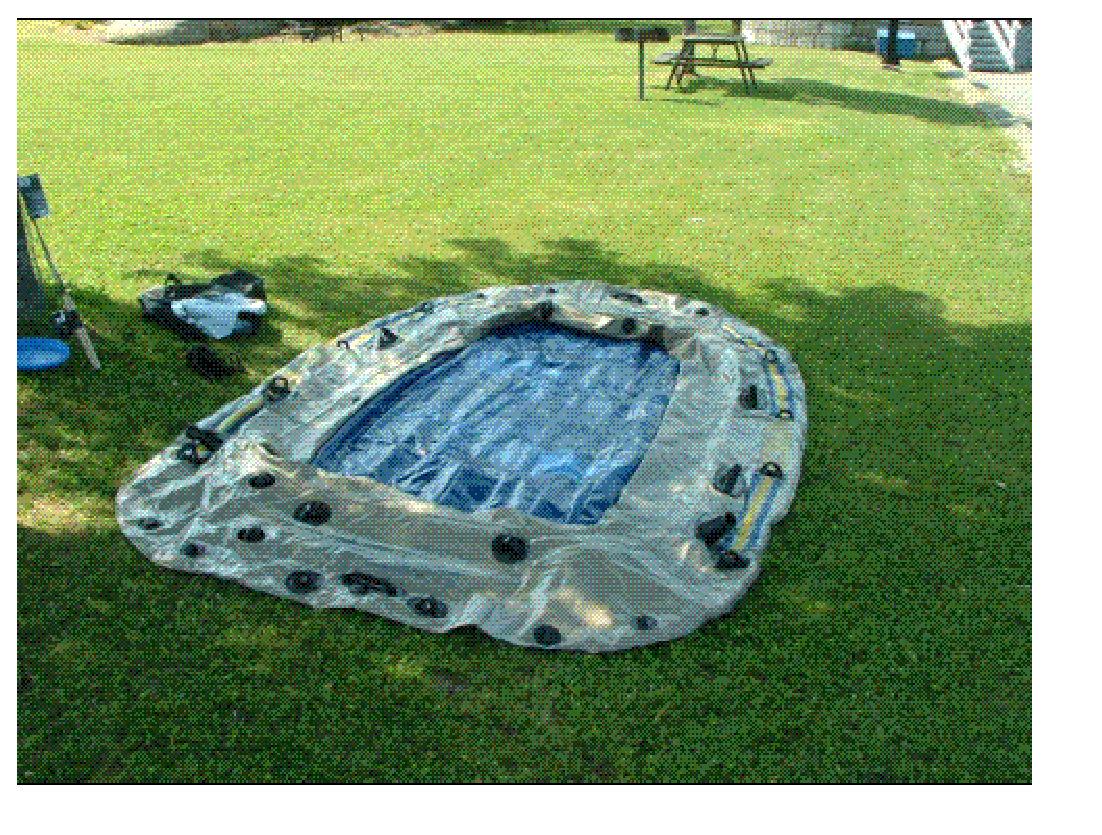
\epsfig{file=fig1.eps,width=3.5in}
Which one of the following is missing in it?
 
 
\noindent{\textbf{\large{
A.}}}
An airplane
 
 
\noindent{\textbf{\large{
B.}}}
An air-boat
 
 
\noindent{\textbf{\large{
C.}}}
Lawn
 
 
\noindent{\textbf{\large{
D.}}}
A frisbee
 
 
\noindent{\textbf{\large{
E.}}}
A truck
 
 
\noindent{\textbf{\large{
F.}}}
  Not any of aboves.
 
 
\noindent\vspace{0.05in}{\textbf{\Large{Auto-answer:}}}
 
 
\noindent{\textbf{\large{
A.}}}
An airplane
 
 
\noindent{\textbf{\large{
E.}}}
A truck
 
 
\noindent\vspace{0.05in}{\textbf{\Large{End of auto-answer.}}}
 
 
 
\vspace{0.3in}
   
   
\noindent{\textbf{\Large{Total numbers: }}}
   
   
\noindent\begin{tabular}{|l|l|l|l|l|l|l|}
 \hline
Inputs & Calculates & Choices & Layers & Matches & Answer & Solution \\ \hline
           0  & 
           0  & 
           6
  simple  
  & 
           6  & 
           0  & 
  yes & 
  no 
  \\ \hline
 \end{tabular}
   
   
   
   
\noindent\vspace{0.1in}{\textbf{\Large{Calculated values:}}}
   
   
   
   
\noindent\vspace{0.1in}\hspace{-0.08in} {\textbf{\Large{All inputs: }}}
   
   
  
\vspace{0.2in}
  
{\textbf{\Large{Question
30.1.2 
 (           6 ,          12 ,          27 )
}}}
  
  
In a hotel, the possiblity of  % 
smoking customer is
$a =  % 
0.730$, and the possiblity of  % 
equal-or-above 30 years old customer is $ b =  % 
0.7600$.
Please fill the following form.
 
\noindent
\begin{tabular}{|l|l|}
\hline
Customer & Possibility \\
\hline
smoking  and   % 
equal-or-above 30 years old  & \\
\hline
smoking  and   % 
under 30 years old & \\
\hline
 non-smoking and   % 
equal-or-above 30 years old  & \\
\hline
 non-smoking and  % 
under 30 years old & \\
\hline
\end{tabular}
 
 
 
 
 
\noindent\vspace{0.1in}{\textbf{\Large{Solution: }}}
 
 

Since the possiblity of  % 
smoking customer is $ a =  % 
0.730 $,
and the possiblity of  % 
equal-or-above 30 years old customer is $ b =  % 
0.7600 $,
the possiblity of  % 
non-smoking customer is $ c = 1.0 - a = 1.0 -
0.730
=  % 
0.270 $ and the possiblity of  % 
under 30 years old
customer is $ d = 1.0 - b = 1.0 -  % 
0.7600 =  % 
0.2400  $.
Then
 
\noindent
\begin{tabular}{|l|l|}
\hline
Customer & Possibility \\
\hline
smoking  and  % 
equal-or-above 30 years old  &
  $ % 
0.730 \times  % 
0.7600 =  % 
0.555$ \\
\hline
smoking  and  % 
under 30 years old &
  $ % 
0.730 \times  % 
0.2400 =  % 
0.175$ \\
\hline
 non-smoking and  % 
equal-or-above 30 years old  &
  $ % 
0.270 \times  % 
0.7600 =  % 
0.205$ \\
\hline
 non-smoking and  % 
under 30 years old &
  $ % 
0.270 \times  % 
0.2400 =  % 
6.48 \times 10^{-2}$ \\
\hline
\end{tabular}
 
\noindent
And the total summation of all possibilities is $  % 
1.000 $.
 
 
 
 
\noindent\vspace{0.1in}{\textbf{\Large{End of Solution.}}}
 
 

 
 
 
\noindent\vspace{0.05in}{\textbf{\Large{Answer:}}}
 
 

 
\noindent
\begin{tabular}{|l|l|}
\hline
Customer & Possibility \\
\hline
smoking  and  % 
equal-or-above 30 years old &
  $ % 
0.555$ \\
\hline
smoking  and  % 
under 30 years old &
  $ % 
0.175$ \\
\hline
 non-smoking and  % 
equal-or-above 30 years old &
  $ % 
0.205$ \\
\hline
 non-smoking and  % 
under 30 years old &
  $ % 
6.48 \times 10^{-2}$ \\
\hline
\end{tabular}
 
\noindent
 And the total summation of all possibilities is $  % 
1.000 $.
 
 
 
\noindent\vspace{0.05in}{\textbf{\Large{End of Answer.}}}
 
 

 
\vspace{0.3in}
   
   
\noindent{\textbf{\Large{Total numbers: }}}
   
   
\noindent\begin{tabular}{|l|l|l|l|l|l|l|}
 \hline
Inputs & Calculates & Choices & Layers & Matches & Answer & Solution \\ \hline
           4  & 
          11  & 
           0
  & 
           0  & 
           0  & 
  yes & 
  yes 
  \\ \hline
 \end{tabular}
   
   
   
   
\noindent\vspace{0.1in}{\textbf{\Large{Calculated values:}}}
   
   
  
  
\noindent\begin{tabular}{|l|l|l|l|}
\hline
 Sequential & Type & Accuracy & Calculated \\ 
\hline
 
 
  Calculated $            1 $ & real & $            3  $ & 
 $ 0.270 $ 
 \\  \hline  
 
 
  Calculated $            2 $ & real & $            4  $ & 
 $ 0.2400 $ 
 \\  \hline  
 
 
  Calculated $            3 $ & real & $            3  $ & 
 $ 0.730 $ 
 \\  \hline  
 
 
  Calculated $            4 $ & real & $            3  $ & 
 $ 0.270 $ 
 \\  \hline  
 
 
  Calculated $            5 $ & real & $            4  $ & 
 $ 0.7600 $ 
 \\  \hline  
 
 
  Calculated $            6 $ & real & $            4  $ & 
 $ 0.2400 $ 
 \\  \hline  
 
 
  Calculated $            7 $ & real & $            3  $ & 
 $ 0.555 $ 
 \\  \hline  
 
 
  Calculated $            8 $ & real & $            3  $ & 
 $ 0.175 $ 
 \\  \hline  
 
 
  Calculated $            9 $ & real & $            3  $ & 
 $ 0.205 $ 
 \\  \hline  
 
 
  Calculated $           10 $ & real & $            3  $ & 
 $ 6.48 \times 10^{-2} $ 
 \\  \hline  
 \end{tabular}
   
   
  
  
\noindent\begin{tabular}{|l|l|l|l|}
\hline
 Sequential & Type & Accuracy & Calculated \\ 
\hline
 
 
  Calculated $           11 $ & real & $            4  $ & 
 $ 1.000 $ 
 \\  \hline  
 \end{tabular}
   
   
   
   
\noindent\vspace{0.1in}\hspace{-0.08in} {\textbf{\Large{All inputs: }}}
   
   
  
  
\noindent\begin{tabular}{|l|l|l|l|l|}
\hline
 Sequential & Type & Accuracy & Three inputs & Generated \\ 
\hline
 
 
  INPUT $            1 $ & logical & .TRUE. & 
 smoking & 
  $ <-- $ 
  \\
  & & .FALSE. & 
  non-smoking & 
 \\  \hline  
 
 
  INPUT $            2 $ & real & $           -3  $ & $
 1.0 \times 10^{-2}
  $ & \\
  & & &  $
 1.000
  $ & \\
  & & &  $
 1.0 \times 10^{-2}
 $ & $ 0.730 $ 
 \\  \hline  
 
 
  INPUT $            3 $ & logical & .TRUE. & 
 equal-or-above 30 years old & 
  $ <-- $ 
  \\
  & & .FALSE. & 
  under 30 years old & 
 \\  \hline  
 \end{tabular}
   
   
  
  
\noindent\begin{tabular}{|l|l|l|l|l|}
\hline
 Sequential & Type & Accuracy & Three inputs & Generated \\ 
\hline
 
 
  INPUT $            4 $ & real & $           -4  $ & $
 2.00 \times 10^{-2}
  $ & \\
  & & &  $
 1.0000
  $ & \\
  & & &  $
 2.00 \times 10^{-2}
 $ & $ 0.7600 $ 
 \\  \hline  
 \end{tabular}
   
   
  
\vspace{0.2in}
  
{\textbf{\Large{Question
30.1.3 
 (           6 ,           6 ,          21 )
}}}
  
  
 
An object is subjected to an external net force $\mathbf{f}=(
80.0,  % 
2.0,
-7000.0  )N$. Its mass is known as
$m= % 
58.0 kg$. Please calculate its accelaration.
 
 
 
 
\noindent\vspace{0.05in}{\textbf{\Large{Answer:}}}
 
 

We will use the Newton's Second Law:
 
\[
\mathbf{f}=m\mathbf{a}.
\]
 
Since $\mathbf{f}=( % 
80.0,  % 
2.0,  % 
-7000.0 )N$
and $m= % 
58.0 kg$, bring them into the above equation, then we get
 
\begin{eqnarray*}
\mathbf{a}&=&\frac{\mathbf{f}}m  \\
&=&\frac{(
80.0 ,
2.0 ,
-7000.0 )N
}{ % 
58.0 kg}  \\
&=&(
1.3793 ,
3.4483 \times 10^{-2},
-120.69
)ms^{-2} \\
&=&(
17876. ,
446.90 ,
-1.5641 \times 10^{6}
)km/h^2.
\end{eqnarray*}
 
 
 
\noindent\vspace{0.05in}{\textbf{\Large{End of Answer.}}}
 
 

 
 
 
\noindent\vspace{0.1in}{\textbf{\Large{Solution: }}}
 
 

We will use the Newton's Second Law:
 
\[
\mathbf{f}=m\mathbf{a}.
\]
 
Since $\mathbf{f}=( % 
80.0,  % 
2.0,  % 
-7000.0 )N$
and $m= % 
58.0 kg$, bring them into the above equation, then we get
 
\begin{eqnarray*}
\mathbf{a}&=&\frac{\mathbf{f}}m  \\
&=&\frac{(
80.0 ,
2.0 ,
-7000.0 )N
}{ % 
58.0 kg}  \\
&=&(
1.3793 ,
3.4483 \times 10^{-2},
-120.69
)ms^{-2} \\
&=&(
17876. ,
446.90 ,
-1.5641 \times 10^{6}
)km/h^2.
\end{eqnarray*}
 
 
 
\noindent\vspace{0.1in}{\textbf{\Large{End of Solution.}}}
 
 

 
\vspace{0.3in}
   
   
\noindent{\textbf{\Large{Total numbers: }}}
   
   
\noindent\begin{tabular}{|l|l|l|l|l|l|l|}
 \hline
Inputs & Calculates & Choices & Layers & Matches & Answer & Solution \\ \hline
           4  & 
           6  & 
           0
  & 
           0  & 
           0  & 
  yes & 
  yes 
  \\ \hline
 \end{tabular}
   
   
   
   
\noindent\vspace{0.1in}{\textbf{\Large{Calculated values:}}}
   
   
  
  
\noindent\begin{tabular}{|l|l|l|l|}
\hline
 Sequential & Type & Accuracy & Calculated \\ 
\hline
 
 
  Calculated $            1 $ & real & $            5  $ & 
 $ 1.3793 $ 
 \\  \hline  
 
 
  Calculated $            2 $ & real & $            5  $ & 
 $ 3.4483 \times 10^{-2} $ 
 \\  \hline  
 
 
  Calculated $            3 $ & real & $            5  $ & 
 $ -120.69 $ 
 \\  \hline  
 
 
  Calculated $            4 $ & real & $            5  $ & 
 $ 17876. $ 
 \\  \hline  
 
 
  Calculated $            5 $ & real & $            5  $ & 
 $ 446.90 $ 
 \\  \hline  
 
 
  Calculated $            6 $ & real & $            5  $ & 
 $ -1.5641 \times 10^{6} $ 
 \\  \hline  
 \end{tabular}
   
   
   
   
\noindent\vspace{0.1in}\hspace{-0.08in} {\textbf{\Large{All inputs: }}}
   
   
  
  
\noindent\begin{tabular}{|l|l|l|l|l|}
\hline
 Sequential & Type & Accuracy & Three inputs & Generated \\ 
\hline
 
 
  INPUT $            1 $ & real & $           -1  $ & $
 20.0
  $ & \\
  & & &  $
 101.0
  $ & \\
  & & &  $
 10.0
 $ & $ 80.0 $ 
 \\  \hline  
 
 
  INPUT $            2 $ & real & $           -1  $ & $
 2.0
  $ & \\
  & & &  $
 10.1
  $ & \\
  & & &  $
 1.0
 $ & $ 2.0 $ 
 \\  \hline  
 
 
  INPUT $            3 $ & real & $           -1  $ & $
 -2000.0
  $ & \\
  & & &  $
 -10001.0
  $ & \\
  & & &  $
 -1000.0
 $ & $ -7000.0 $ 
 \\  \hline  
 \end{tabular}
   
   
  
  
\noindent\begin{tabular}{|l|l|l|l|l|}
\hline
 Sequential & Type & Accuracy & Three inputs & Generated \\ 
\hline
 
 
  INPUT $            4 $ & real & $           -1  $ & $
 50.0
  $ & \\
  & & &  $
 60.1
  $ & \\
  & & &  $
 2.0
 $ & $ 58.0 $ 
 \\  \hline  
 \end{tabular}
   
   
  
\vspace{0.2in}
  
{\textbf{\Large{Question
30.1.4 
 (           6 ,           9 ,          24 )
}}}
  
  
Let us use Newton's Law of Universal Gravitation to calculate the force
of the Sun acting on the eight planets. Let us suppose the mass of the
Sun is $ % 
3.00 \times 10^{24} kg$. With the mass and the
distance to the Sun of each planet in the following table, please fill
the blanks for the forces.
 
\vspace{0.2in}
 
 
\begin{tabular}{|l|l|l|l|}
\hline
The Planet & Mass ($kg$) & Distanace from Sun ($m$) & The Force ($N$)\\
\hline
Mercury  &
           $ % 
3.00000000 \times 10^{24} $   &
             $ % 
7.000000000 \times 10^{24} $    &
\\  \hline
Venus    &
           $ % 
3.00 \times 10^{24} $    &
             $ % 
5.00 \times 10^{24} $    &
\\  \hline
Earth    &
           $ % 
9.00 \times 10^{24} $    &
             $ % 
8.00 \times 10^{24} $    &
\\   \hline
Mars     &
           $ % 
9.00 \times 10^{24} $    &
             $ % 
3.00 \times 10^{24} $    &
\\   \hline
Jupiter  &
           $ % 
7.00 \times 10^{24} $    &
             $ % 
5.00 \times 10^{24} $    &
\\  \hline
Saturn   &
           $ % 
1.000 \times 10^{25}$    &
             $ % 
8.00 \times 10^{24}$    &
\\  \hline
Uranus   &
           $ % 
6.00 \times 10^{24} $    &
             $ % 
9.00 \times 10^{24} $    &
\\  \hline
Neptune  &
           $ % 
6.00 \times 10^{24} $    &
             $ % 
7.00 \times 10^{24} $    &
\\  \hline
 
\end{tabular}
 
 
 
 
\noindent\vspace{0.1in}{\textbf{\Large{Solution: }}}
 
 

By using Newton's Law of Universal Gravitation:
\[
F=G \frac{(Sun's \hspace{0.1in} mass) \times (Planet's \hspace{0.1in} mass)} { (distance)^2},
\]
where
$ G= % 
6.67 \times 10^{-11}N m^{2}(kg)^{-2}$ , the forces can be easily calculated as
 
\vspace{0.2in}
 
 
\begin{tabular}{|l|l|l|l|}
\hline
The Planet & Mass ($kg$) & Distanace from Sun ($m$) & The Force ($N$)\\
\hline
Mercury  &
           $ % 
3.00000000 \times 10^{24} $   &
             $ % 
7.000000000 \times 10^{24} $    & $ % 
1.23 \times 10^{-11} $
\\  \hline
Venus    &
           $  % 
3.00 \times 10^{24}  $     &
             $ % 
5.00 \times 10^{24} $    & $ % 
2.40 \times 10^{-11} $
\\  \hline
Earth    &
           $  % 
9.00 \times 10^{24}  $     &
             $ % 
8.00 \times 10^{24} $    & $ % 
2.81 \times 10^{-11} $
\\   \hline
Mars     &
           $  % 
9.00 \times 10^{24} $     &
             $ % 
3.00 \times 10^{24} $    & $ % 
2.00 \times 10^{-10} $
\\   \hline
Jupiter  &
           $  % 
7.00 \times 10^{24} $    &
             $ % 
5.00 \times 10^{24} $    & $ % 
5.60 \times 10^{-11} $
\\  \hline
Saturn   &
           $  % 
1.000 \times 10^{25} $    &
             $ % 
8.00 \times 10^{24}  $    & $ % 
3.13 \times 10^{-11} $
\\  \hline
Uranus   &
           $  % 
6.00 \times 10^{24} $    &
             $ % 
9.00 \times 10^{24} $    & $ % 
1.48 \times 10^{-11} $
\\  \hline
Neptune  &
           $  % 
6.00 \times 10^{24} $    &
             $ % 
7.00 \times 10^{24} $    & $ % 
2.45 \times 10^{-11} $
\\  \hline
 
\end{tabular}
 
 
 
 
\noindent\vspace{0.1in}{\textbf{\Large{End of Solution.}}}
 
 

 
 
 
 
\noindent\vspace{0.05in}{\textbf{\Large{Answer:}}}
 
 

By using Newton's Law of Universal Gravitation:
\[
F=G \frac{(Sun's \hspace{0.1in} mass) \times (Planet's \hspace{0.1in} mass)} { (distance)^2},
\]
where
$ G= % 
6.67 \times 10^{-11} N m^{2}(kg)^{-2}$ , the forces can be easily calculated as
 
\vspace{0.2in}
 
 
\begin{tabular}{|l|l|l|l|}
\hline
The Planet & Mass ($kg$) & Distanace from Sun ($m$) & The Force ($N$)\\
\hline
Mercury  &
           $ % 
3.00000000 \times 10^{24}  $   &
             $ % 
7.000000000 \times 10^{24}$    & $ % 
1.23 \times 10^{-11} $
\\  \hline
Venus    &
           $  % 
3.00 \times 10^{24}  $     &
             $ % 
5.00 \times 10^{24} $    & $ % 
2.40 \times 10^{-11} $
\\  \hline
Earth    &
           $  % 
9.00 \times 10^{24}$     &
             $ % 
8.00 \times 10^{24} $    & $ % 
2.81 \times 10^{-11} $
\\   \hline
Mars     &
           $  % 
9.00 \times 10^{24} $     &
             $ % 
3.00 \times 10^{24}$    & $ % 
2.00 \times 10^{-10} $
\\   \hline
Jupiter  &
           $  % 
7.00 \times 10^{24}  $    &
             $ % 
5.00 \times 10^{24} $    & $ % 
5.60 \times 10^{-11}3 $
\\  \hline
Saturn   &
           $  % 
1.000 \times 10^{25}   $    &
             $ % 
8.00 \times 10^{24}  $    & $ % 
3.13 \times 10^{-11} $
\\  \hline
Uranus   &
           $  % 
6.00 \times 10^{24} $    &
             $ % 
9.00 \times 10^{24}$    & $ % 
1.48 \times 10^{-11} $
\\  \hline
Neptune  &
           $  % 
6.00 \times 10^{24}  $    &
             $ % 
7.00 \times 10^{24} $    & $ % 
2.45 \times 10^{-11} $
\\  \hline
 
\end{tabular}
 
 
 
 
\noindent\vspace{0.05in}{\textbf{\Large{End of Answer.}}}
 
 

 
\vspace{0.3in}
   
   
\noindent{\textbf{\Large{Total numbers: }}}
   
   
\noindent\begin{tabular}{|l|l|l|l|l|l|l|}
 \hline
Inputs & Calculates & Choices & Layers & Matches & Answer & Solution \\ \hline
          19  & 
           8  & 
           0
  & 
           0  & 
           0  & 
  yes & 
  yes 
  \\ \hline
 \end{tabular}
   
   
   
   
\noindent\vspace{0.1in}{\textbf{\Large{Calculated values:}}}
   
   
  
  
\noindent\begin{tabular}{|l|l|l|l|}
\hline
 Sequential & Type & Accuracy & Calculated \\ 
\hline
 
 
  Calculated $            1 $ & real & $            3  $ & 
 $ 1.23 \times 10^{-11} $ 
 \\  \hline  
 
 
  Calculated $            2 $ & real & $            3  $ & 
 $ 2.40 \times 10^{-11} $ 
 \\  \hline  
 
 
  Calculated $            3 $ & real & $            3  $ & 
 $ 2.81 \times 10^{-11} $ 
 \\  \hline  
 
 
  Calculated $            4 $ & real & $            3  $ & 
 $ 2.00 \times 10^{-10} $ 
 \\  \hline  
 
 
  Calculated $            5 $ & real & $            3  $ & 
 $ 5.60 \times 10^{-11} $ 
 \\  \hline  
 
 
  Calculated $            6 $ & real & $            3  $ & 
 $ 3.13 \times 10^{-11} $ 
 \\  \hline  
 
 
  Calculated $            7 $ & real & $            3  $ & 
 $ 1.48 \times 10^{-11} $ 
 \\  \hline  
 
 
  Calculated $            8 $ & real & $            3  $ & 
 $ 2.45 \times 10^{-11} $ 
 \\  \hline  
 \end{tabular}
   
   
   
   
\noindent\vspace{0.1in}\hspace{-0.08in} {\textbf{\Large{All inputs: }}}
   
   
  
  
\noindent\begin{tabular}{|l|l|l|l|l|}
\hline
 Sequential & Type & Accuracy & Three inputs & Generated \\ 
\hline
 
 
  INPUT $            1 $ & real & $           22  $ & $
 2.00 \times 10^{24}
  $ & \\
  & & &  $
 1.010 \times 10^{25}
  $ & \\
  & & &  $
 1.00 \times 10^{24}
 $ & $ 3.00 \times 10^{24} $ 
 \\  \hline  
 
 
  INPUT $            2 $ & real & $           16  $ & $
 2.00000000 \times 10^{24}
  $ & \\
  & & &  $
 1.010000000 \times 10^{25}
  $ & \\
  & & &  $
 1.00000000 \times 10^{24}
 $ & $ 3.00000000 \times 10^{24} $ 
 \\  \hline  
 
 
  INPUT $            3 $ & real & $           15  $ & $
 2.000000000 \times 10^{24}
  $ & \\
  & & &  $
 1.0100000000 \times 10^{25}
  $ & \\
  & & &  $
 1.000000000 \times 10^{24}
 $ & $ 7.000000000 \times 10^{24} $ 
 \\  \hline  
 \end{tabular}
   
   
  
  
\noindent\begin{tabular}{|l|l|l|l|l|}
\hline
 Sequential & Type & Accuracy & Three inputs & Generated \\ 
\hline
 
 
  INPUT $            4 $ & real & $           22  $ & $
 2.00 \times 10^{24}
  $ & \\
  & & &  $
 1.010 \times 10^{25}
  $ & \\
  & & &  $
 1.00 \times 10^{24}
 $ & $ 3.00 \times 10^{24} $ 
 \\  \hline  
 
 
  INPUT $            5 $ & real & $           22  $ & $
 2.00 \times 10^{24}
  $ & \\
  & & &  $
 1.010 \times 10^{25}
  $ & \\
  & & &  $
 1.00 \times 10^{24}
 $ & $ 5.00 \times 10^{24} $ 
 \\  \hline  
 
 
  INPUT $            6 $ & real & $           22  $ & $
 2.00 \times 10^{24}
  $ & \\
  & & &  $
 1.010 \times 10^{25}
  $ & \\
  & & &  $
 1.00 \times 10^{24}
 $ & $ 9.00 \times 10^{24} $ 
 \\  \hline  
 \end{tabular}
   
   
  
  
\noindent\begin{tabular}{|l|l|l|l|l|}
\hline
 Sequential & Type & Accuracy & Three inputs & Generated \\ 
\hline
 
 
  INPUT $            7 $ & real & $           22  $ & $
 2.00 \times 10^{24}
  $ & \\
  & & &  $
 1.010 \times 10^{25}
  $ & \\
  & & &  $
 1.00 \times 10^{24}
 $ & $ 8.00 \times 10^{24} $ 
 \\  \hline  
 
 
  INPUT $            8 $ & real & $           22  $ & $
 2.00 \times 10^{24}
  $ & \\
  & & &  $
 1.010 \times 10^{25}
  $ & \\
  & & &  $
 1.00 \times 10^{24}
 $ & $ 9.00 \times 10^{24} $ 
 \\  \hline  
 
 
  INPUT $            9 $ & real & $           22  $ & $
 2.00 \times 10^{24}
  $ & \\
  & & &  $
 1.010 \times 10^{25}
  $ & \\
  & & &  $
 1.00 \times 10^{24}
 $ & $ 3.00 \times 10^{24} $ 
 \\  \hline  
 \end{tabular}
   
   
  
  
\noindent\begin{tabular}{|l|l|l|l|l|}
\hline
 Sequential & Type & Accuracy & Three inputs & Generated \\ 
\hline
 
 
  INPUT $           10 $ & real & $           22  $ & $
 2.00 \times 10^{24}
  $ & \\
  & & &  $
 1.010 \times 10^{25}
  $ & \\
  & & &  $
 1.00 \times 10^{24}
 $ & $ 7.00 \times 10^{24} $ 
 \\  \hline  
 
 
  INPUT $           11 $ & real & $           22  $ & $
 2.00 \times 10^{24}
  $ & \\
  & & &  $
 1.010 \times 10^{25}
  $ & \\
  & & &  $
 1.00 \times 10^{24}
 $ & $ 5.00 \times 10^{24} $ 
 \\  \hline  
 
 
  INPUT $           12 $ & real & $           22  $ & $
 2.00 \times 10^{24}
  $ & \\
  & & &  $
 1.010 \times 10^{25}
  $ & \\
  & & &  $
 1.00 \times 10^{24}
 $ & $ 1.000 \times 10^{25} $ 
 \\  \hline  
 \end{tabular}
   
   
  
  
\noindent\begin{tabular}{|l|l|l|l|l|}
\hline
 Sequential & Type & Accuracy & Three inputs & Generated \\ 
\hline
 
 
  INPUT $           13 $ & real & $           22  $ & $
 2.00 \times 10^{24}
  $ & \\
  & & &  $
 1.010 \times 10^{25}
  $ & \\
  & & &  $
 1.00 \times 10^{24}
 $ & $ 8.00 \times 10^{24} $ 
 \\  \hline  
 
 
  INPUT $           14 $ & real & $           22  $ & $
 2.00 \times 10^{24}
  $ & \\
  & & &  $
 1.010 \times 10^{25}
  $ & \\
  & & &  $
 1.00 \times 10^{24}
 $ & $ 6.00 \times 10^{24} $ 
 \\  \hline  
 
 
  INPUT $           15 $ & real & $           22  $ & $
 2.00 \times 10^{24}
  $ & \\
  & & &  $
 1.010 \times 10^{25}
  $ & \\
  & & &  $
 1.00 \times 10^{24}
 $ & $ 9.00 \times 10^{24} $ 
 \\  \hline  
 \end{tabular}
   
   
  
  
\noindent\begin{tabular}{|l|l|l|l|l|}
\hline
 Sequential & Type & Accuracy & Three inputs & Generated \\ 
\hline
 
 
  INPUT $           16 $ & real & $           22  $ & $
 2.00 \times 10^{24}
  $ & \\
  & & &  $
 1.010 \times 10^{25}
  $ & \\
  & & &  $
 1.00 \times 10^{24}
 $ & $ 6.00 \times 10^{24} $ 
 \\  \hline  
 
 
  INPUT $           17 $ & real & $           22  $ & $
 2.00 \times 10^{24}
  $ & \\
  & & &  $
 1.010 \times 10^{25}
  $ & \\
  & & &  $
 1.00 \times 10^{24}
 $ & $ 7.00 \times 10^{24} $ 
 \\  \hline  
 
 
  INPUT $           18 $ & real & $          -13  $ & $
 6.67 \times 10^{-11}
  $ & \\
  & & &  $
 6.67 \times 10^{-11}
  $ & \\
  & & &  $
 1.00 \times 10^{-11}
 $ & $ 6.67 \times 10^{-11} $ 
 \\  \hline  
 \end{tabular}
   
   
  
  
\noindent\begin{tabular}{|l|l|l|l|l|}
\hline
 Sequential & Type & Accuracy & Three inputs & Generated \\ 
\hline
 
 
  INPUT $           19 $ & real & $          -13  $ & $
 6.67 \times 10^{-11}
  $ & \\
  & & &  $
 6.67 \times 10^{-11}
  $ & \\
  & & &  $
 1.00 \times 10^{-11}
 $ & $ 6.67 \times 10^{-11} $ 
 \\  \hline  
 \end{tabular}
   
   
  
\vspace{0.2in}
  
{\textbf{\Large{Question
30.1.5 
 (           6 ,           8 ,          23 )
}}}
  
  
 
An object is subjected to an external net force $\mathbf{f}=(
60.0 ,
6.0,
-3000.0  )N$. Its mass is known as
$m= % 
56.0  kg$. Please choose the correct accelaration
from the following choices.
 
 
 
\noindent{\textbf{\large{
A.}}}
The accelaration is
$(
2.9098ms^{-2},
0.10714ms^{-2},
1.9567 \times 10^{6}km/h^2
).
$
 
 
\noindent{\textbf{\large{
B.}}}
The accelaration is
$(
1.0714ms^{-2},
0.46937ms^{-2},
-694286.km/h^2
).
$
 
 
\noindent{\textbf{\large{
C.}}}
The accelaration is
$(
1.0714ms^{-2},
0.10714ms^{-2},
-694286.km/h^2
).
$
 
 
\noindent{\textbf{\large{
D.}}}
The accelaration is
$(
2.9098ms^{-2},
0.46937ms^{-2},
1.9567 \times 10^{6}km/h^2
).
$
 
 
\noindent{\textbf{\large{
E.}}}
none of these.
 
 
\noindent\vspace{0.05in}{\textbf{\Large{Auto-answer:}}}
 
 
\noindent{\textbf{\large{
C.}}}
The accelaration is
$(
1.0714ms^{-2},
0.10714ms^{-2},
-694286.km/h^2
).
$
 
 
\noindent\vspace{0.05in}{\textbf{\Large{End of auto-answer.}}}
 
 
 
 
 
 
\noindent\vspace{0.1in}{\textbf{\Large{Solution: }}}
 
 

We will use the Newton's Second Law:
 
\[
\mathbf{f}=m\mathbf{a}.
\]
 
Since $\mathbf{f}=( % 
60.0,  % 
6.0,  % 
-3000.0 )N$
and $m= % 
56.0kg$, bring them into the above equation, then we get
 
\begin{eqnarray*}
\mathbf{a}&=&\frac{\mathbf{f}}m  \\
&=&\frac{(
60.0 ,
6.0 ,
-3000.0 )N
}{ % 
56.0 kg}  \\
&=&(
1.0714 ,
0.10714,
-53.571
)ms^{-2} \\
&=&(
13886. ,
1388.6 ,
-694286.
)km/h^2.
\end{eqnarray*}
 
 
 
\noindent\vspace{0.1in}{\textbf{\Large{End of Solution.}}}
 
 

 
\vspace{0.3in}
   
   
\noindent{\textbf{\Large{Total numbers: }}}
   
   
\noindent\begin{tabular}{|l|l|l|l|l|l|l|}
 \hline
Inputs & Calculates & Choices & Layers & Matches & Answer & Solution \\ \hline
           4  & 
           6  & 
           5
  & 
           3  & 
           0  & 
  yes & 
  yes 
  \\ \hline
 \end{tabular}
   
   
   
   
\noindent\vspace{0.1in}{\textbf{\Large{Calculated values:}}}
   
   
  
  
\noindent\begin{tabular}{|l|l|l|l|}
\hline
 Sequential & Type & Accuracy & Calculated \\ 
\hline
 
 
  Calculated $            1 $ & real & $            5  $ & 
 $ 1.0714 $ 
 \\  \hline  
 
 
  Calculated $            2 $ & real & $            5  $ & 
 $ 0.10714 $ 
 \\  \hline  
 
 
  Calculated $            3 $ & real & $            5  $ & 
 $ -53.571 $ 
 \\  \hline  
 
 
  Calculated $            4 $ & real & $            5  $ & 
 $ 13886. $ 
 \\  \hline  
 
 
  Calculated $            5 $ & real & $            5  $ & 
 $ 1388.6 $ 
 \\  \hline  
 
 
  Calculated $            6 $ & real & $            5  $ & 
 $ -694286. $ 
 \\  \hline  
 \end{tabular}
   
   
   
   
\noindent\vspace{0.1in}\hspace{-0.08in} {\textbf{\Large{All inputs: }}}
   
   
  
  
\noindent\begin{tabular}{|l|l|l|l|l|}
\hline
 Sequential & Type & Accuracy & Three inputs & Generated \\ 
\hline
 
 
  INPUT $            1 $ & real & $           -1  $ & $
 20.0
  $ & \\
  & & &  $
 101.0
  $ & \\
  & & &  $
 10.0
 $ & $ 60.0 $ 
 \\  \hline  
 
 
  INPUT $            2 $ & real & $           -1  $ & $
 2.0
  $ & \\
  & & &  $
 10.1
  $ & \\
  & & &  $
 1.0
 $ & $ 6.0 $ 
 \\  \hline  
 
 
  INPUT $            3 $ & real & $           -1  $ & $
 -2000.0
  $ & \\
  & & &  $
 -10001.0
  $ & \\
  & & &  $
 -1000.0
 $ & $ -3000.0 $ 
 \\  \hline  
 \end{tabular}
   
   
  
  
\noindent\begin{tabular}{|l|l|l|l|l|}
\hline
 Sequential & Type & Accuracy & Three inputs & Generated \\ 
\hline
 
 
  INPUT $            4 $ & real & $           -1  $ & $
 50.0
  $ & \\
  & & &  $
 60.1
  $ & \\
  & & &  $
 2.0
 $ & $ 56.0 $ 
 \\  \hline  
 \end{tabular}
   
   
  
\vspace{0.2in}
  
{\textbf{\Large{Question
30.1.6 
 (           6 ,           7 ,          22 )
}}}
  
  
 
An object is subjected to an external net force $\mathbf{f}=(
30.0 ,
2.0,
-6000.0  )N$. Its mass is known as
$m= % 
54.0  kg$. Please choose the correct accelaration
from the following choices.
 
 
 
\noindent{\textbf{\large{
A.}}}
The accelaration (vector) is
$(
7200.0,
480.00 ,
-4.7594 \times 10^{6}
)km/h^2.
$
 
 
\noindent{\textbf{\large{
B.}}}
The accelaration (vector) is
$(
7200.0,
480.00 ,
-1.4400 \times 10^{6}
)km/h^2.
$
 
 
\noindent{\textbf{\large{
C.}}}
The accelaration (vector) is
$(
27380.,
480.00 ,
3.7975 \times 10^{6}
)km/h^2.
$
 
 
\noindent{\textbf{\large{
D.}}}
The accelaration (vector) is
$(
-20827.,
480.00 ,
7.0625 \times 10^{6}
)km/h^2.
$
 
 
\noindent{\textbf{\large{
E.}}}
The accelaration (vector) is
$(
27380.,
480.00 ,
-4.7594 \times 10^{6}
)km/h^2.
$
 
 
\noindent{\textbf{\large{
F.}}}
The accelaration (vector) is
$(
-20827.,
480.00 ,
3.7975 \times 10^{6}
)km/h^2.
$
 
 
\noindent{\textbf{\large{
G.}}}
The accelaration (vector) is
$(
27380.,
480.00 ,
-1.4400 \times 10^{6}
)km/h^2.
$
 
 
\noindent{\textbf{\large{
H.}}}
The accelaration (vector) is
$(
31230.,
480.00 ,
-1.4400 \times 10^{6}
)km/h^2.
$
 
 
\noindent{\textbf{\large{
I.}}}
The accelaration (vector) is
$(
7200.0,
480.00 ,
7.0625 \times 10^{6}
)km/h^2.
$
 
 
\noindent{\textbf{\large{
J.}}}
The accelaration (vector) is
$(
27380.,
480.00 ,
7.0625 \times 10^{6}
)km/h^2.
$
 
 
\noindent{\textbf{\large{
K.}}}
The accelaration (vector) is
$(
31230.,
480.00 ,
3.7975 \times 10^{6}
)km/h^2.
$
 
 
\noindent{\textbf{\large{
L.}}}
The accelaration (vector) is
$(
7200.0,
480.00 ,
3.7975 \times 10^{6}
)km/h^2.
$
 
 
\noindent\vspace{0.05in}{\textbf{\Large{Auto-answer:}}}
 
 
\noindent{\textbf{\large{
B.}}}
The accelaration (vector) is
$(
7200.0,
480.00 ,
-1.4400 \times 10^{6}
)km/h^2.
$
 
 
\noindent\vspace{0.05in}{\textbf{\Large{End of auto-answer.}}}
 
 
 
 
 
 
\noindent\vspace{0.1in}{\textbf{\Large{Solution: }}}
 
 

We will use the Newton's Second Law:
 
\[
\mathbf{f}=m\mathbf{a}.
\]
 
Since $\mathbf{f}=( % 
30.0,  % 
2.0,  % 
-6000.0 )N$
and $m= % 
54.0 kg$, bring them into the above equation, then we get
 
\begin{eqnarray*}
\mathbf{a}&=&\frac{\mathbf{f}}m  \\
&=&\frac{(
30.0 ,
2.0 ,
-6000.0 )N
}{ % 
54.0 kg}  \\
&=&(
0.55556 ,
3.7037 \times 10^{-2},
-111.11
)ms^{-2} \\
&=&(
7200.0 ,
480.00 ,
-1.4400 \times 10^{6}
)km/h^2.
\end{eqnarray*}
 
 
 
\noindent\vspace{0.1in}{\textbf{\Large{End of Solution.}}}
 
 

 
 
\vspace{0.3in}
   
   
\noindent{\textbf{\Large{Total numbers: }}}
   
   
\noindent\begin{tabular}{|l|l|l|l|l|l|l|}
 \hline
Inputs & Calculates & Choices & Layers & Matches & Answer & Solution \\ \hline
           4  & 
           6  & 
          12
  & 
           2  & 
           0  & 
  yes & 
  yes 
  \\ \hline
 \end{tabular}
   
   
   
   
\noindent\vspace{0.1in}{\textbf{\Large{Calculated values:}}}
   
   
  
  
\noindent\begin{tabular}{|l|l|l|l|}
\hline
 Sequential & Type & Accuracy & Calculated \\ 
\hline
 
 
  Calculated $            1 $ & real & $            5  $ & 
 $ 0.55556 $ 
 \\  \hline  
 
 
  Calculated $            2 $ & real & $            5  $ & 
 $ 3.7037 \times 10^{-2} $ 
 \\  \hline  
 
 
  Calculated $            3 $ & real & $            5  $ & 
 $ -111.11 $ 
 \\  \hline  
 
 
  Calculated $            4 $ & real & $            5  $ & 
 $ 7200.0 $ 
 \\  \hline  
 
 
  Calculated $            5 $ & real & $            5  $ & 
 $ 480.00 $ 
 \\  \hline  
 
 
  Calculated $            6 $ & real & $            5  $ & 
 $ -1.4400 \times 10^{6} $ 
 \\  \hline  
 \end{tabular}
   
   
   
   
\noindent\vspace{0.1in}\hspace{-0.08in} {\textbf{\Large{All inputs: }}}
   
   
  
  
\noindent\begin{tabular}{|l|l|l|l|l|}
\hline
 Sequential & Type & Accuracy & Three inputs & Generated \\ 
\hline
 
 
  INPUT $            1 $ & real & $           -1  $ & $
 20.0
  $ & \\
  & & &  $
 101.0
  $ & \\
  & & &  $
 10.0
 $ & $ 30.0 $ 
 \\  \hline  
 
 
  INPUT $            2 $ & real & $           -1  $ & $
 2.0
  $ & \\
  & & &  $
 10.1
  $ & \\
  & & &  $
 1.0
 $ & $ 2.0 $ 
 \\  \hline  
 
 
  INPUT $            3 $ & real & $           -1  $ & $
 -2000.0
  $ & \\
  & & &  $
 -10001.0
  $ & \\
  & & &  $
 -1000.0
 $ & $ -6000.0 $ 
 \\  \hline  
 \end{tabular}
   
   
  
  
\noindent\begin{tabular}{|l|l|l|l|l|}
\hline
 Sequential & Type & Accuracy & Three inputs & Generated \\ 
\hline
 
 
  INPUT $            4 $ & real & $           -1  $ & $
 50.0
  $ & \\
  & & &  $
 60.1
  $ & \\
  & & &  $
 2.0
 $ & $ 54.0 $ 
 \\  \hline  
 \end{tabular}
   
   
   
   
\vspace{0.3in}
{\textbf{\LARGE{You have done all the above? A very good beginning, please go ahead.}}}
More constants the
Mass of electron
$m_e$$ =
9.109390 \times 10^{-31} $
kg
,
Universal gas constant
$R$$ =
8.315 $
J/(mol$\cdot $K)
,
$e$$ =
1.60217733 \times 10^{-19} $
C
, and
$m_p$$ =
1.6726231 \times 10^{-27} $
kg
%
may be very helpful.
\vspace{0.3in}
   
   
  
\vspace{0.2in}
  
{\textbf{\Large{QUESTION
30.2 
 (           5 ,           5 ,           5 )
}}}
  
  
If any one of the following statements is correct, please fill the box ahead of it with $T$ .
If wrong, fill with $F$.
 
\noindent\begin{tabular}{|l|l|}\hline Your&\hspace{.2in} \\ answer&\hspace{.2in} \\ \hline \end{tabular}
1. $ % 
28$ is an  % 
even number.
 
\noindent\begin{tabular}{|l|l|}\hline Your&\hspace{.2in} \\ answer&\hspace{.2in} \\ \hline \end{tabular}
2.  % 
Montreal is in  % 
Ontario province.
 
\noindent\begin{tabular}{|l|l|}\hline Your&\hspace{.2in} \\ answer&\hspace{.2in} \\ \hline \end{tabular}
3.  % 
$\mathbf{F}=m\mathbf{a}$ is a mathmatical form of
the Newton's Second Law.
 
 
 
\noindent\vspace{0.05in}{\textbf{\Large{Answer:}}}
 
 

 
\noindent\begin{tabular}{|l|l|}\hline The correct & \\
          answer &  % 
$T$ \\ \hline \end{tabular}
1. $ % 
28$ is an  % 
even number.
 
\noindent\begin{tabular}{|l|l|}\hline The correct & \\
          answer &  % 
$F$ \\ \hline \end{tabular}
2.  % 
Montreal is in  % 
Ontario province.
 
\noindent\begin{tabular}{|l|l|}\hline The correct & \\
          answer &  % 
$T$ \\ \hline \end{tabular}
3.  % 
$\mathbf{F}=m\mathbf{a}$ is a mathmatical form of  % 
the Newton's Second Law.
 
 
 
\noindent\vspace{0.05in}{\textbf{\Large{End of Answer.}}}
 
 

 
\vspace{0.3in}
   
   
\noindent{\textbf{\Large{Total numbers: }}}
   
   
\noindent\begin{tabular}{|l|l|l|l|l|l|l|}
 \hline
Inputs & Calculates & Choices & Layers & Matches & Answer & Solution \\ \hline
           6  & 
           3  & 
           0
  & 
           0  & 
           0  & 
  yes & 
  no 
  \\ \hline
 \end{tabular}
   
   
   
   
\noindent\vspace{0.1in}{\textbf{\Large{Calculated values:}}}
   
   
  
  
\noindent\begin{tabular}{|l|l|l|l|}
\hline
 Sequential & Type & Accuracy & Calculated \\ 
\hline
 
 
  Calculated $            1 $ & string & $            1  $ ( $           1  $ strings): 
 & $T$
 \\  \hline  
 
 
  Calculated $            2 $ & string & $            1  $ ( $           1  $ strings): 
 & $F$
 \\  \hline  
 
 
  Calculated $            3 $ & string & $            1  $ ( $           1  $ strings): 
 & $T$
 \\  \hline  
 \end{tabular}
   
   
   
   
\noindent\vspace{0.1in}\hspace{-0.08in} {\textbf{\Large{All inputs: }}}
   
   
  
  
\noindent\begin{tabular}{|l|l|l|l|l|}
\hline
 Sequential & Type & Accuracy & Three inputs & Generated \\ 
\hline
 
 
  INPUT $            1 $ & integer &  & $
 1
 , 
 100
 , 
 1
 $ & $ 28 $ 
 \\  \hline  
 
 
  INPUT $            2 $ & string & & 
 even & 
  $ <-- $ 
  \\
  & & & 
 odd & 
 \\  \hline  
 
 
  INPUT $            3 $ & string & & 
 Toronto & 
  \\
  & & & 
 Kingston & 
  \\
  & & & 
 Montreal & 
  $ <-- $ 
  \\
  & & & 
 Hull & 
 \\  \hline  
 \end{tabular}
   
   
  
  
\noindent\begin{tabular}{|l|l|l|l|l|}
\hline
 Sequential & Type & Accuracy & Three inputs & Generated \\ 
\hline
 
 
  INPUT $            4 $ & string & & 
 Ontario & 
  $ <-- $ 
  \\
  & & & 
 Quebec & 
 \\  \hline  
 
 
  INPUT $            5 $ & string & & 
 $\mathbf{F}=m\mathbf{a}$ & 
  $ <-- $ 
  \\
  & & & 
 $\left| \mathbf{F}\right| =Gm_1m_2r^{-2}$ & 
 \\  \hline  
 
 
  INPUT $            6 $ & string & & 
 the Newton's Second Law & 
  $ <-- $ 
  \\
  & & & 
 Newton's Law of Universal Gravitation & 
 \\  \hline  
 \end{tabular}
   
   
  
\vspace{0.2in}
  
{\textbf{\Large{QUESTION
30.3 
 (           3 ,           3 ,           3 )
}}}
  
  
Please choose the correct one from the following statements:
 
 
\noindent{\textbf{\large{
A.}}}
Canada has  %
33 provinces and  %
38 territories.
 
 
\noindent{\textbf{\large{
B.}}}
Canada has  %
35 provinces and  %
34 territories.
 
 
\noindent{\textbf{\large{
C.}}}
Canada has  %
37 provinces and  %
37 territories.
 
 
\noindent{\textbf{\large{
D.}}}
Canada has  %
36 provinces and  %
35 territories.
 
 
\noindent{\textbf{\large{
E.}}}
Canada has  %
34 provinces and  %
39 territories.
 
 
\noindent{\textbf{\large{
F.}}}
 None of above.
 
 
\noindent\vspace{0.05in}{\textbf{\Large{Auto-answer:}}}
 
 
\noindent{\textbf{\large{
F.}}}
 None of above.
 
 
\noindent\vspace{0.05in}{\textbf{\Large{End of auto-answer.}}}
 
 
   
   
\noindent{\textbf{\Large{Total numbers: }}}
   
   
\noindent\begin{tabular}{|l|l|l|l|l|l|l|}
 \hline
Inputs & Calculates & Choices & Layers & Matches & Answer & Solution \\ \hline
           0  & 
          20  & 
           6
  simple  
  & 
           6  & 
           0  & 
  yes & 
  no 
  \\ \hline
 \end{tabular}
   
   
   
   
\noindent\vspace{0.1in}{\textbf{\Large{Calculated values:}}}
   
   
  
  
\noindent\begin{tabular}{|l|l|l|l|}
\hline
 Sequential & Type & Accuracy & Calculated \\ 
\hline
 
 
  Calculated $            1 $ & integer &  & 
  $ 10 $ 
 \\  \hline  
 
 
  Calculated $            2 $ & integer &  & 
  $ 3 $ 
 \\  \hline  
 
 
  Calculated $            3 $ & integer &  & 
  $ 23 $ 
 \\  \hline  
 
 
  Calculated $            4 $ & integer &  & 
  $ 24 $ 
 \\  \hline  
 
 
  Calculated $            5 $ & integer &  & 
  $ 25 $ 
 \\  \hline  
 
 
  Calculated $            6 $ & integer &  & 
  $ 26 $ 
 \\  \hline  
 
 
  Calculated $            7 $ & integer &  & 
  $ 27 $ 
 \\  \hline  
 
 
  Calculated $            8 $ & integer &  & 
  $ 28 $ 
 \\  \hline  
 
 
  Calculated $            9 $ & integer &  & 
  $ 29 $ 
 \\  \hline  
 
 
  Calculated $           10 $ & integer &  & 
  $ 30 $ 
 \\  \hline  
 \end{tabular}
   
   
  
  
\noindent\begin{tabular}{|l|l|l|l|}
\hline
 Sequential & Type & Accuracy & Calculated \\ 
\hline
 
 
  Calculated $           11 $ & integer &  & 
  $ 31 $ 
 \\  \hline  
 
 
  Calculated $           12 $ & integer &  & 
  $ 32 $ 
 \\  \hline  
 
 
  Calculated $           13 $ & integer &  & 
  $ 33 $ 
 \\  \hline  
 
 
  Calculated $           14 $ & integer &  & 
  $ 34 $ 
 \\  \hline  
 
 
  Calculated $           15 $ & integer &  & 
  $ 35 $ 
 \\  \hline  
 
 
  Calculated $           16 $ & integer &  & 
  $ 36 $ 
 \\  \hline  
 
 
  Calculated $           17 $ & integer &  & 
  $ 37 $ 
 \\  \hline  
 
 
  Calculated $           18 $ & integer &  & 
  $ 38 $ 
 \\  \hline  
 
 
  Calculated $           19 $ & integer &  & 
  $ 39 $ 
 \\  \hline  
 
 
  Calculated $           20 $ & integer &  & 
  $ 40 $ 
 \\  \hline  
 \end{tabular}
   
   
   
   
\noindent\vspace{0.1in}\hspace{-0.08in} {\textbf{\Large{All inputs: }}}
   
   
  
\vspace{0.2in}
  
{\textbf{\Large{QUESTION
30.4 
 (           1 ,           1 ,           1 )
}}}
  
  


\noindent\vspace{0.05in}{\textbf{\Large{Abstract:}}}
This is a simple Newton's Second Law calculation multi-choice problem.  
\noindent\vspace{0.05in}{\textbf{\Large{end of abstract.}}}


 
 
An object is subjected to an external net force $\mathbf{f}=
(20.0 , 4.0 , -6000.0) N$.
Its mass is known as $m= % 
52.0000 kg$. Please choose the
correct accelaration from the following choices.
 
 
 
\noindent{\textbf{\large{
A.}}}
The accelaration is $  %
(
0.385,
7.7 \times 10^{-2},
526.04)
ms^{-2} $.
 
 
\noindent{\textbf{\large{
B.}}}
The accelaration is $  %
(
0.385,
7.7 \times 10^{-2},
-115.38)
ms^{-2} $.
 
 
\noindent{\textbf{\large{
C.}}}
The accelaration is $  %
(
0.385,
0.23,
-115.38)
ms^{-2} $.
 
 
\noindent{\textbf{\large{
D.}}}
The accelaration is $  %
(
4.34,
7.7 \times 10^{-2},
-115.38)
ms^{-2} $.
 
 
\noindent{\textbf{\large{
E.}}}
The accelaration is $  %
(
4.34,
0.23,
526.04)
ms^{-2} $.
 
 
\noindent{\textbf{\large{
F.}}}
The accelaration is $  %
(
0.385,
0.23,
526.04)
ms^{-2} $.
 
 
\noindent{\textbf{\large{
G.}}}
The accelaration is $  %
(
4.34,
7.7 \times 10^{-2},
526.04)
ms^{-2} $.
 
 
\noindent{\textbf{\large{
H.}}}
The accelaration is $  %
(
4.34,
0.23,
-115.38)
ms^{-2} $.
 
 
\noindent\vspace{0.05in}{\textbf{\Large{Auto-answer:}}}
 
 
\noindent{\textbf{\large{
B.}}}
The accelaration is $  %
(
0.385,
7.7 \times 10^{-2},
-115.38)
ms^{-2} $.
 
 
\noindent\vspace{0.05in}{\textbf{\Large{End of auto-answer.}}}
 
 
 
 
 
\noindent\vspace{0.05in}{\textbf{\Large{Answer:}}}
 
 

The correct answer from the choices is


\noindent{\textbf{\large{
B.}}}
The accelaration is $  %
(
0.385,
7.7 \times 10^{-2},
-115.38)
ms^{-2} $.
 
 
 
\noindent\vspace{0.05in}{\textbf{\Large{End of Answer.}}}
 
 

 
 
 
\noindent\vspace{0.1in}{\textbf{\Large{Solution: }}}
 
 

We will use the Newton's Second Law:
 
\[
\mathbf{f}=m\mathbf{a}.
\]
 
Since $\mathbf{f}= % 
(20.0 , 4.0 , -6000.0) N$
and $m= % 
52.0000kg$, bring them into the above equation, then we get
 
\begin{eqnarray*}
\mathbf{a}&=&\frac{\mathbf{f}}m  \\
&=&\frac{ % 
(20.0 , 4.0 , -6000.0) N}{ % 
52.0000kg}  \\
&=& % 
(0.385 , 7.7 \times 10^{-2} , -115.38) ms^{-2}
\end{eqnarray*}
 
 
 
\noindent\vspace{0.1in}{\textbf{\Large{End of Solution.}}}
 
 

 
\vspace{0.3in}
   
   
\noindent{\textbf{\Large{Total numbers: }}}
   
   
\noindent\begin{tabular}{|l|l|l|l|l|l|l|}
 \hline
Inputs & Calculates & Choices & Layers & Matches & Answer & Solution \\ \hline
           2  & 
           1  & 
           8
  & 
           3  & 
           0  & 
  yes & 
  yes 
  \\ \hline
 \end{tabular}
   
   
   
   
\noindent\vspace{0.1in}{\textbf{\Large{Calculated values:}}}
   
   
  
  
\noindent\begin{tabular}{|l|l|l|l|}
\hline
 Sequential & Type & Accuracy & Calculated \\ 
\hline
 
 
  Calculated $            1 $ & vector &  
  $            3  $ 
 &  $ 0.385 $ 
 \\    
  & & 
  $            2  $ 
 &  $ 7.7 \times 10^{-2} $ 
 \\    
  & & 
  $            5  $ 
 &  $ -115.38 $ 
 \\  \hline  
 \end{tabular}
   
   
   
   
\noindent\vspace{0.1in}\hspace{-0.08in} {\textbf{\Large{All inputs: }}}
   
   
  
  
\noindent\begin{tabular}{|l|l|l|l|l|}
\hline
 Sequential & Type & Accuracy & Three inputs & Generated \\ 
\hline
 
 
  INPUT $            1 $ & vector & $           -1  $ & $
20.0
  $ & \\
  & & & $
101.0
  $ & \\
  & & & $
10.0
$ & $ 20.0 $ 
  \\
  & & $           -1  $ & $
2.0
  $ & \\
  & & & $
10.1
  $ & \\
  & & & $
1.0
$ & $ 4.0 $ 
  \\
  & & $           -1  $ & $
-2000.0
  $ & \\
  & & & $
-10001.0
  $ & \\
  & & & $
-1000.0
$ & $ -6000.0 $ 
 \\  \hline  
 
 
  INPUT $            2 $ & real & $           -4  $ & $
 50.0000
  $ & \\
  & & &  $
 60.1000
  $ & \\
  & & &  $
 2.0000
 $ & $ 52.0000 $ 
 \\  \hline  
 \end{tabular}
   
   
  
\vspace{0.2in}
  
{\textbf{\Large{QUESTION
30.5 
 (           4 ,           4 ,           4 )
}}}
  
  
Considering case-insensitivity, please match the following same strings.
  
  
\begin{tabular}{|l|l|l|}
 \hline
 Column Left & Column Right  & Your choinces \\ 
 \hline
{\textbf{\large{
A.}}}
A
  & 
b
 & 
 \\ 
 \hline
{\textbf{\large{
B.}}}
 A= %
6/ %
2

  & 
ER
 & 
 \\ 
 \hline
{\textbf{\large{
C.}}}
Er
  & 
eR
 & 
 \\ 
 \hline
{\textbf{\large{
D.}}}
B
  & 
 a= %
3
 & 
 \\ 
 \hline
{\textbf{\large{
E.}}}
er
  & 
a
 & 
 \\ 
 \hline
 \end{tabular}
  
  
 
 
\noindent\vspace{0.05in}{\textbf{\Large{Auto-answer:}}}
  
  
\begin{tabular}{|l|l|l|}
 \hline
 Column Left & Column Right  & Answers       \\ 
 \hline
{\textbf{\large{
A.}}}
A
  & 
b
 & 
{\textbf{\large{
D.}}}
 \\ 
 \hline
{\textbf{\large{
B.}}}
 A= %
6/ %
2

  & 
ER
 & 
{\textbf{\large{
C.}}}
, 
{\textbf{\large{
E.}}}
 \\ 
 \hline
{\textbf{\large{
C.}}}
Er
  & 
eR
 & 
{\textbf{\large{
C.}}}
, 
{\textbf{\large{
E.}}}
 \\ 
 \hline
{\textbf{\large{
D.}}}
B
  & 
 a= %
3
 & 
{\textbf{\large{
B.}}}
 \\ 
 \hline
{\textbf{\large{
E.}}}
er
  & 
a
 & 
{\textbf{\large{
A.}}}
 \\ 
 \hline
 \end{tabular}
  
  
 
 
\noindent\vspace{0.05in}{\textbf{\Large{End of auto-answer.}}}
 
 
 
   
   
\noindent{\textbf{\Large{Total numbers: }}}
   
   
\noindent\begin{tabular}{|l|l|l|l|l|l|l|}
 \hline
Inputs & Calculates & Choices & Layers & Matches & Answer & Solution \\ \hline
           2  & 
           1  & 
           0
  & 
          16  & 
           5  & 
  yes & 
  no 
  \\ \hline
 \end{tabular}
   
   
   
   
\noindent\vspace{0.1in}{\textbf{\Large{Calculated values:}}}
   
   
  
  
\noindent\begin{tabular}{|l|l|l|l|}
\hline
 Sequential & Type & Accuracy & Calculated \\ 
\hline
 
 
  Calculated $            1 $ & integer &  & 
  $ 3 $ 
 \\  \hline  
 \end{tabular}
   
   
   
   
\noindent\vspace{0.1in}\hspace{-0.08in} {\textbf{\Large{All inputs: }}}
   
   
  
  
\noindent\begin{tabular}{|l|l|l|l|l|}
\hline
 Sequential & Type & Accuracy & Three inputs & Generated \\ 
\hline
 
 
  INPUT $            1 $ & integer &  & $
 2
 , 
 8
 , 
 2
 $ & $ 6 $ 
 \\  \hline  
 
 
  INPUT $            2 $ & integer &  & $
 2
 , 
 3
 , 
 2
 $ & $ 2 $ 
 \\  \hline  
 \end{tabular}
   
   
  
\vspace{0.2in}
  
{\textbf{\Large{QUESTION
30.6 
 (           2 ,           2 ,           2 )
}}}
  
  
 
An object is subjected to an external net force $\mathbf{f}=(
20.000 ,
3.0000,
-2000.0  )N$. Its mass is known as
$m= % 
60.0000  kg$. Please choose the correct accelaration
from the following choices.
 
 
 
\noindent{\textbf{\large{
A.}}}
The accelaration is
$(
0.33333ms^{-2},
648.00km/h^2,
116.36ms^{-2}
).
$
 
 
\noindent{\textbf{\large{
B.}}}
The accelaration is
$(
0.33333ms^{-2},
648.00km/h^2,
-33.333ms^{-2}
).
$
 
 
\noindent{\textbf{\large{
C.}}}
The accelaration is
$(
0.33333ms^{-2},
1945.9km/h^2,
-33.333ms^{-2}
).
$
 
 
\noindent{\textbf{\large{
D.}}}
The accelaration is
$(
-0.96447ms^{-2},
1945.9km/h^2,
-33.333ms^{-2}
).
$
 
 
\noindent{\textbf{\large{
E.}}}
The accelaration is
$(
-0.96447ms^{-2},
648.00km/h^2,
-33.333ms^{-2}
).
$
 
 
\noindent{\textbf{\large{
F.}}}
The accelaration is
$(
0.33333ms^{-2},
1945.9km/h^2,
116.36ms^{-2}
).
$
 
 
\noindent{\textbf{\large{
G.}}}
 None of these.
 
 
\noindent\vspace{0.05in}{\textbf{\Large{Auto-answer:}}}
 
 
\noindent{\textbf{\large{
B.}}}
The accelaration is
$(
0.33333ms^{-2},
648.00km/h^2,
-33.333ms^{-2}
).
$
 
 
\noindent\vspace{0.05in}{\textbf{\Large{End of auto-answer.}}}
 
 
 
 
 
 
\noindent\vspace{0.1in}{\textbf{\Large{Solution: }}}
 
 

We will use the Newton's Second Law:
 
\[
\mathbf{f}=m\mathbf{a}.
\]
 
Since $\mathbf{f}=( % 
20.000,  % 
3.0000,  % 
-2000.0 )N$
and $m= % 
60.0000kg$, bring them into the above equation, then we get
 
\begin{eqnarray*}
\mathbf{a}&=&\frac{\mathbf{f}}m  \\
&=&\frac{(
20.000 ,
3.0000 ,
-2000.0 )N
}{ % 
60.0000 kg}  \\
&=&(
0.33333 ,
5.0000 \times 10^{-2},
-33.333
)ms^{-2} \\
&=&(
4320.0 ,
648.00 ,
-432000.
)km/h^2.
\end{eqnarray*}
 
 
 
\noindent\vspace{0.1in}{\textbf{\Large{End of Solution.}}}
 
 

 
\vspace{0.3in}
   
   
\noindent{\textbf{\Large{Total numbers: }}}
   
   
\noindent\begin{tabular}{|l|l|l|l|l|l|l|}
 \hline
Inputs & Calculates & Choices & Layers & Matches & Answer & Solution \\ \hline
           4  & 
           6  & 
           7
  & 
           3  & 
           0  & 
  yes & 
  yes 
  \\ \hline
 \end{tabular}
   
   
   
   
\noindent\vspace{0.1in}{\textbf{\Large{Calculated values:}}}
   
   
  
  
\noindent\begin{tabular}{|l|l|l|l|}
\hline
 Sequential & Type & Accuracy & Calculated \\ 
\hline
 
 
  Calculated $            1 $ & real & $            5  $ & 
 $ 0.33333 $ 
 \\  \hline  
 
 
  Calculated $            2 $ & real & $            5  $ & 
 $ 5.0000 \times 10^{-2} $ 
 \\  \hline  
 
 
  Calculated $            3 $ & real & $            5  $ & 
 $ -33.333 $ 
 \\  \hline  
 
 
  Calculated $            4 $ & real & $            5  $ & 
 $ 4320.0 $ 
 \\  \hline  
 
 
  Calculated $            5 $ & real & $            5  $ & 
 $ 648.00 $ 
 \\  \hline  
 
 
  Calculated $            6 $ & real & $            5  $ & 
 $ -432000. $ 
 \\  \hline  
 \end{tabular}
   
   
   
   
\noindent\vspace{0.1in}\hspace{-0.08in} {\textbf{\Large{All inputs: }}}
   
   
  
  
\noindent\begin{tabular}{|l|l|l|l|l|}
\hline
 Sequential & Type & Accuracy & Three inputs & Generated \\ 
\hline
 
 
  INPUT $            1 $ & real & $           -3  $ & $
 20.000
  $ & \\
  & & &  $
 101.000
  $ & \\
  & & &  $
 10.000
 $ & $ 20.000 $ 
 \\  \hline  
 
 
  INPUT $            2 $ & real & $           -4  $ & $
 2.0000
  $ & \\
  & & &  $
 10.1000
  $ & \\
  & & &  $
 1.0000
 $ & $ 3.0000 $ 
 \\  \hline  
 
 
  INPUT $            3 $ & real & $           -1  $ & $
 -2000.0
  $ & \\
  & & &  $
 -10001.0
  $ & \\
  & & &  $
 -1000.0
 $ & $ -2000.0 $ 
 \\  \hline  
 \end{tabular}
   
   
  
  
\noindent\begin{tabular}{|l|l|l|l|l|}
\hline
 Sequential & Type & Accuracy & Three inputs & Generated \\ 
\hline
 
 
  INPUT $            4 $ & real & $           -4  $ & $
 50.0000
  $ & \\
  & & &  $
 60.1000
  $ & \\
  & & &  $
 2.0000
 $ & $ 60.0000 $ 
 \\  \hline  
 \end{tabular}
   
   
   
   
\vspace{0.3in}
{\textbf{\LARGE{You have done all the above? Excellent! Not much left, please continue.}}}
\vspace{0.3in}
   
   
  
\vspace{0.2in}
  
{\textbf{\Large{QUESTION
30.7 
 (           7 ,          14 ,          50 )
}}}
  
  
 
An object is subjected to an external net force $\mathbf{f}=
(60.0 , 3.0 , -6000.0) N$.
Its mass is known as $m= % 
54.0 kg$.
Please choose the correct accelaration from the following choices.
 
 
\noindent{\textbf{\large{
A.}}}
  The accelaration is $  %
(
1.11,
5.6 \times 10^{-2},
-111.11)
ms^{-2} $.
 
 
\noindent{\textbf{\large{
B.}}}
  The accelaration is $  %
(
3.83,
5.6 \times 10^{-2},
-111.11)
ms^{-2} $.
 
 
\noindent{\textbf{\large{
C.}}}
  The accelaration is $  %
(
1.11,
5.6 \times 10^{-2},
356.81)
ms^{-2} $.
 
 
\noindent{\textbf{\large{
D.}}}
  The accelaration is $  %
(
3.83,
0.19,
356.81)
ms^{-2} $.
 
 
\noindent\vspace{0.05in}{\textbf{\Large{Auto-answer:}}}
 
 
\noindent{\textbf{\large{
A.}}}
  The accelaration is $  %
(
1.11,
5.6 \times 10^{-2},
-111.11)
ms^{-2} $.
 
 
\noindent\vspace{0.05in}{\textbf{\Large{End of auto-answer.}}}
 
 
 
 
 
\noindent\vspace{0.1in}{\textbf{\Large{Solution: }}}
 
 

We will use the Newton's Second Law:
 
\[
\mathbf{f}=m\mathbf{a}.
\]
 
Since $\mathbf{f}= % 
(60.0 , 3.0 , -6000.0) N$
and $m= % 
54.0kg$, bring them into the above equation, then we get
 
\begin{eqnarray*}
\mathbf{a}&=&\frac{\mathbf{f}}m  \\
&=&\frac{ % 
(60.0 , 3.0 , -6000.0) N}{ % 
54.0kg}  \\
&=& % 
(1.11 , 5.6 \times 10^{-2} , -111.11) ms^{-2}
\end{eqnarray*}
 
 
 
\noindent\vspace{0.1in}{\textbf{\Large{End of Solution.}}}
 
 

 
 
\vspace{0.3in}
   
   
\noindent{\textbf{\Large{Total numbers: }}}
   
   
\noindent\begin{tabular}{|l|l|l|l|l|l|l|}
 \hline
Inputs & Calculates & Choices & Layers & Matches & Answer & Solution \\ \hline
           2  & 
           1  & 
           4
  & 
           3  & 
           0  & 
  yes & 
  yes 
  \\ \hline
 \end{tabular}
   
   
   
   
\noindent\vspace{0.1in}{\textbf{\Large{Calculated values:}}}
   
   
  
  
\noindent\begin{tabular}{|l|l|l|l|}
\hline
 Sequential & Type & Accuracy & Calculated \\ 
\hline
 
 
  Calculated $            1 $ & vector &  
  $            3  $ 
 &  $ 1.11 $ 
 \\    
  & & 
  $            2  $ 
 &  $ 5.6 \times 10^{-2} $ 
 \\    
  & & 
  $            5  $ 
 &  $ -111.11 $ 
 \\  \hline  
 \end{tabular}
   
   
   
   
\noindent\vspace{0.1in}\hspace{-0.08in} {\textbf{\Large{All inputs: }}}
   
   
  
  
\noindent\begin{tabular}{|l|l|l|l|l|}
\hline
 Sequential & Type & Accuracy & Three inputs & Generated \\ 
\hline
 
 
  INPUT $            1 $ & vector & $           -1  $ & $
20.0
  $ & \\
  & & & $
101.0
  $ & \\
  & & & $
10.0
$ & $ 60.0 $ 
  \\
  & & $           -1  $ & $
2.0
  $ & \\
  & & & $
10.1
  $ & \\
  & & & $
1.0
$ & $ 3.0 $ 
  \\
  & & $           -1  $ & $
-2000.0
  $ & \\
  & & & $
-10001.0
  $ & \\
  & & & $
-1000.0
$ & $ -6000.0 $ 
 \\  \hline  
 
 
  INPUT $            2 $ & real & $           -1  $ & $
 50.0
  $ & \\
  & & &  $
 60.1
  $ & \\
  & & &  $
 2.0
 $ & $ 54.0 $ 
 \\  \hline  
 \end{tabular}
   
   
  
\vspace{0.2in}
  
{\textbf{\Large{QUESTION
30.8 
 (           8 ,          15 ,          60 )
}}}
  
  
 
$ \left( \begin{array}{ccccccccc}
           4  & 
           6  & 
           7  & 
           5  \\ 
           5  & 
           4  & 
           5  & 
           6  \\ 
           5  & 
           4  & 
           5  & 
           6
\end{array}\right) \times
\left( \begin{array}{c}
           2  \\ 
           2  \\ 
           2  \\ 
           2
\end{array}\right) $ =?
 
 
$  % 
 \left( \begin{array}
 {
 c
 c
 }
 \Lambda & 
 \Psi \\ 
 \sigma & 
 \Upsilon \\ 
 \beta & 
 \beta \\ 
 \Phi & 
 \Theta
 \end{array} \right)
 \left( \begin{array}
 {
 c
 }
 \beta \\ 
 \beta
 \end{array} \right)
$ =?
 
 
 
\noindent\vspace{0.05in}{\textbf{\Large{Answer:}}}
 
 

 
$\left( \begin{array}{ccccccccccccccc}
           4  & 
           6  & 
           7  & 
           5  \\ 
           5  & 
           4  & 
           5  & 
           6  \\ 
           5  & 
           4  & 
           5  & 
           6
\end{array}\right) \times
\left( \begin{array}{c}
           2  \\ 
           2  \\ 
           2  \\ 
           2
\end{array}\right)  =
\left( \begin{array}{c}
          44  \\ 
          40  \\ 
          40
\end{array}\right)  $
 
$  % 
 \left( \begin{array}
 {
 c
 c
 }
 \Lambda & 
 \Psi \\ 
 \sigma & 
 \Upsilon \\ 
 \beta & 
 \beta \\ 
 \Phi & 
 \Theta
 \end{array} \right)
 \left( \begin{array}
 {
 c
 }
 \beta \\ 
 \beta
 \end{array} \right)
=
 \left( \begin{array}
 {
 c
 }
  \Lambda \times  \beta +  \Psi \times  \beta \\ 
  \sigma \times  \beta +  \Upsilon \times  \beta \\ 
  \beta \times  \beta +  \beta \times  \beta \\ 
  \Phi \times  \beta +  \Theta \times  \beta
 \end{array} \right)
$
 
 
 
\noindent\vspace{0.05in}{\textbf{\Large{End of Answer.}}}
 
 

 
 
 
\noindent\vspace{0.1in}{\textbf{\Large{Solution: }}}
 
 

 
 
\noindent\vspace{0.1in}{\textbf{\Large{End of Solution.}}}
 
 

 
\vspace{0.3in}
   
   
\noindent{\textbf{\Large{Total numbers: }}}
   
   
\noindent\begin{tabular}{|l|l|l|l|l|l|l|}
 \hline
Inputs & Calculates & Choices & Layers & Matches & Answer & Solution \\ \hline
           4  & 
           2  & 
           0
  & 
           0  & 
           0  & 
  yes & 
  yes 
  \\ \hline
 \end{tabular}
   
   
   
   
\noindent\vspace{0.1in}{\textbf{\Large{Calculated values:}}}
   
   
  
  
\noindent\begin{tabular}{|l|l|l|l|}
\hline
 Sequential & Type & Accuracy & Calculated \\ 
\hline
 
 
  Calculated $            1 $ & i-matrix &  & 
 (size:            3  by            1 )
 \\  \hline  
 \end{tabular}
   
   
$\begin{array}{
 c
 }
          44  \\ 
          40  \\ 
          40
 \end{array}  $ 
  
  
\noindent\begin{tabular}{|l|l|l|l|}
\hline
 Sequential & Type & Accuracy & Calculated \\ 
\hline
 
 
  Calculated $            2 $ & s-matrix & & 
 (size:            4  by            1 )
 \\  \hline  
 \end{tabular}
   
   
 $  \left( \begin{array}
 {
 c
 }
  \Lambda \times  \beta +  \Psi \times  \beta \\ 
  \sigma \times  \beta +  \Upsilon \times  \beta \\ 
  \beta \times  \beta +  \beta \times  \beta \\ 
  \Phi \times  \beta +  \Theta \times  \beta
 \end{array} \right) $ 
   
   
\noindent\vspace{0.1in}\hspace{-0.08in} {\textbf{\Large{All inputs: }}}
   
   
  
  
\noindent\begin{tabular}{|l|l|l|l|l|}
\hline
 Sequential & Type & Accuracy & Three inputs & Generated \\ 
\hline
 
 
  INPUT $            1 $ & i-matrix &  & $
 4
 , 
 7
 , 
 1
 $ & (size:            3  by            4 )
 \\  \hline  
 \end{tabular}
   
   
 $\begin{array}{
 c
 c
 c
 c
 }
           4  & 
           6  & 
           7  & 
           5  \\ 
           5  & 
           4  & 
           5  & 
           6  \\ 
           5  & 
           4  & 
           5  & 
           6
\end{array}  $ 
  
  
\noindent\begin{tabular}{|l|l|l|l|l|}
\hline
 Sequential & Type & Accuracy & Three inputs & Generated \\ 
\hline
 
 
  INPUT $            2 $ & i-matrix &  & $
 2
 , 
 2
 , 
 1
 $ & (size:            4  by            1 )
 \\  \hline  
 \end{tabular}
   
   
 $\begin{array}{
 c
 }
           2  \\ 
           2  \\ 
           2  \\ 
           2
\end{array}  $ 
  
  
\noindent\begin{tabular}{|l|l|l|l|l|}
\hline
 Sequential & Type & Accuracy & Three inputs & Generated \\ 
\hline
 
 
  INPUT $            3 $ & s-matrix & & 
 $  \alpha $ & 
  \\
  & & & 
 $  \beta $ & 
  \\
  & & & 
 $  \gamma $ & 
  \\
  & & & 
 $  \delta $ & 
  \\
  & & & 
 $  \epsilon $ & 
  \\
  & & & 
 $  \varepsilon $ & 
  \\
  & & & 
 $                     \zeta $ & 
  \\
  & & & 
 $  \eta $ & 
  \\
  & & & 
 $  \rho $ & 
  \\
  & & & 
 $  \sigma $ & 
  \\
  & & & 
 $  \Gamma $ & 
  \\
  & & & 
 $  \Delta $ & 
  \\
  & & & 
 $  \Theta $ & 
  \\
  & & & 
 $  \Lambda $ & 
  \\
  & & & 
 $                     \Xi $ & 
  \\
  & & & 
 $  \Upsilon $ & 
  \\
  & & & 
 $  \Phi $ & 
  \\
  & & & 
 $  \Psi $ & 
  \\
  & & & 
 $  \Omega $ & 
  (size:            4  by            2 )
 \\  \hline  
 \end{tabular}
   
   
 $  \left( \begin{array}
 {
 c
 c
 }
 \Lambda & 
 \Psi \\ 
 \sigma & 
 \Upsilon \\ 
 \beta & 
 \beta \\ 
 \Phi & 
 \Theta
 \end{array} \right) $ 
  
  
\noindent\begin{tabular}{|l|l|l|l|l|}
\hline
 Sequential & Type & Accuracy & Three inputs & Generated \\ 
\hline
 
 
  INPUT $            4 $ & s-matrix & & 
 $  \beta $ & 
  \\
  & & & 
 $  \gamma $ & 
  (size:            2  by            1 )
 \\  \hline  
 \end{tabular}
   
   
 $  \left( \begin{array}
 {
 c
 }
 \beta \\ 
 \beta
 \end{array} \right) $ 
  
\vspace{0.2in}
  
{\textbf{\Large{QUESTION
30.9 
 (           9 ,          16 ,          70 )
}}}
  
  


\noindent\vspace{0.05in}{\textbf{\Large{Abstract:}}}
Quadratic Equation constructed from the following first two random (input) integers as roots,  
which of course should not show in the exam papers.  
\noindent\vspace{0.05in}{\textbf{\Large{end of abstract.}}}


 
 
% First root
% Second root

 
Please solve the following equation:
\begin{eqnarray*}
-9 \times x^2  % 
+  % 
63
                 \times x    % 
+  % 
1530 =0
\end{eqnarray*}
 
 
 
\noindent\vspace{0.05in}{\textbf{\Large{Answer:}}}
 
 

17,  % 
-10
 
 
 
\noindent\vspace{0.05in}{\textbf{\Large{End of Answer.}}}
 
 

 
 
 
\noindent\vspace{0.1in}{\textbf{\Large{Solution: }}}
 
 

Roots to the equation
\begin{eqnarray*}
-9 \times x^2  % 
+  % 
63
                 \times x    % 
+  % 
1530 =0
\end{eqnarray*}
are  % 
17 and  % 
-10 .
 
Let us verity  % 
17 first:
$  % 
-9 \times x^2  % 
+  % 
63
                 \times x    % 
+  % 
1530
  = % 
-2601+( % 
1071)+( % 
1530)
  = % 
-1530+( % 
1530)
  = % 
0
$
 
Then verity  % 
-10:
$  % 
-9 \times x^2  % 
+  % 
63
                 \times x    % 
+  % 
1530
  = % 
-900+( % 
-630)+( % 
1530)
  = % 
-1530+( % 
1530)
  = % 
0
$
 
 
 
\noindent\vspace{0.1in}{\textbf{\Large{End of Solution.}}}
 
 

 
\vspace{0.3in}
   
   
\noindent{\textbf{\Large{Total numbers: }}}
   
   
\noindent\begin{tabular}{|l|l|l|l|l|l|l|}
 \hline
Inputs & Calculates & Choices & Layers & Matches & Answer & Solution \\ \hline
           3  & 
          13  & 
           0
  & 
           0  & 
           0  & 
  yes & 
  yes 
  \\ \hline
 \end{tabular}
   
   
   
   
\noindent\vspace{0.1in}{\textbf{\Large{Calculated values:}}}
   
   
  
  
\noindent\begin{tabular}{|l|l|l|l|}
\hline
 Sequential & Type & Accuracy & Calculated \\ 
\hline
 
 
  Calculated $            1 $ & integer &  & 
  $ -9 $ 
 \\  \hline  
 
 
  Calculated $            2 $ & string & $            1  $ ( $           1  $ strings): 
 & +
 \\  \hline  
 
 
  Calculated $            3 $ & integer &  & 
  $ 63 $ 
 \\  \hline  
 
 
  Calculated $            4 $ & string & $            1  $ ( $           1  $ strings): 
 & +
 \\  \hline  
 
 
  Calculated $            5 $ & integer &  & 
  $ 1530 $ 
 \\  \hline  
 
 
  Calculated $            6 $ & integer &  & 
  $ -2601 $ 
 \\  \hline  
 
 
  Calculated $            7 $ & integer &  & 
  $ 1071 $ 
 \\  \hline  
 
 
  Calculated $            8 $ & integer &  & 
  $ -1530 $ 
 \\  \hline  
 
 
  Calculated $            9 $ & integer &  & 
  $ 0 $ 
 \\  \hline  
 
 
  Calculated $           10 $ & integer &  & 
  $ -900 $ 
 \\  \hline  
 \end{tabular}
   
   
  
  
\noindent\begin{tabular}{|l|l|l|l|}
\hline
 Sequential & Type & Accuracy & Calculated \\ 
\hline
 
 
  Calculated $           11 $ & integer &  & 
  $ -630 $ 
 \\  \hline  
 
 
  Calculated $           12 $ & integer &  & 
  $ -1530 $ 
 \\  \hline  
 
 
  Calculated $           13 $ & integer &  & 
  $ 0 $ 
 \\  \hline  
 \end{tabular}
   
   
   
   
\noindent\vspace{0.1in}\hspace{-0.08in} {\textbf{\Large{All inputs: }}}
   
   
  
  
\noindent\begin{tabular}{|l|l|l|l|l|}
\hline
 Sequential & Type & Accuracy & Three inputs & Generated \\ 
\hline
 
 
  INPUT $            1 $ & integer &  & $
 -11
 , 
 30
 , 
 4
 $ & $ 17 $ 
 \\  \hline  
 
 
  INPUT $            2 $ & integer &  & $
 -31
 , 
 60
 , 
 3
 $ & $ -10 $ 
 \\  \hline  
 
 
  INPUT $            3 $ & integer &  & $
 -15
 , 
 15
 , 
 2
 $ & $ -9 $ 
 \\  \hline  
 \end{tabular}
   
   
   
   
   
   
 \vspace{0.2in}
Here are still some constants for use:
 
 
\noindent\begin{tabular}{|l|l|l|}
\hline
Constant & Symbol & Value \\
\hline
 
Mass of proton &
$m_p$ &
 $ 1.6726231 \times 10^{-27} $
kg \\
\hline
 
Boltzmann's constant &
$k$ &
 $ 1.381 \times 10^{-23} $
J/K \\
\hline
 
\end{tabular}
 
Thank you very much for answering these questions!
 
{\textbf{\large{Please be advised}}} that in this paper there are questions from
30.1 through
30.9.
And any one of them may contain more than one sub-question, thus the total number
of sub-questions here is around 14, of which
13 should be answered.
 
   
   
\vspace{2.0in} PAPER TAIL GENERATED.
   
   
   
   
\vspace{1.0in} 
{\textbf{\large{ *** END OF PAPER, THANKS *** }}} 
   
   
\hspace{1.0in} By: 
         239 (          26 ,           34 )
   
   
   
   
\newpage 
\setcounter{page}{ 
    31001 } 
   
   
\noindent{\textbf{\huge{THIS IS THE JOURNAL FOR}}}
   
   
 {\textbf{ \Large{ PAPER NUMBER           31  }}}
   
   
\vspace{0.2in}
   
   
\markboth{Journal NOT for examinees !!! {\today}}{Journal NOT for examinees !!! {\today}}
   
   
   
   
   
   
 \vspace{0.2in}
 
 
{\Huge  THIS IS AN EXAMPLE OF}
 
{\Huge  PERSONALIZED TESTS. }
 
If needed, please use the following constants.
 
 
 
\noindent\begin{tabular}{|l|l|l|}
\hline
Constant & Symbol & Value \\
\hline
Acceleration due to earth's gravity &
$g$ &
 $ 9.80 $
m/s$^2$ \\
\hline
Avogadro's number &
$N_A$ &
 $ 6.0221367 \times 10^{23} $
mol$^{-1}$ \\
\hline
Boltzmann's constant &
$k$ &
 $ 1.380658 \times 10^{-23} $
J/K \\
\hline
Coulomb's constant &
$k$ &
 $ 8.99 \times 10^{9} $
N$\cdot $m$^2$/C$^2$ \\
\hline
Electron charge magnitiude &
$e$ &
 $ 1.60217733 \times 10^{-19} $
C \\
\hline
Permeability of free space &
$\mu _0$ &
 $ 1.25663706 \times 10^{-6} $
T$\cdot $m/A \\
\hline
Permittivity of free space &
$\epsilon _0$ &
 $ 8.854187817 \times 10^{-12} $
C$^2$/(N$\cdot $m$^2$) \\
\hline
Pi &
$\pi$ &
 $ 3.14159265 $
$ $ \\
\hline
Planck's constant &
$h$ &
 $ 6.6260755 \times 10^{-34} $
J$\cdot $s \\
\hline
Mass of electron &
$m_e$ &
 $ 9.1093897 \times 10^{-31} $
kg \\
\hline
\end{tabular}
 
 
\noindent\begin{tabular}{|l|l|l|}
\hline
Constant & Symbol & Value \\
\hline
Mass of neutron &
$m_n$ &
 $ 1.6749286 \times 10^{-27} $
kg \\
\hline
Mass of proton &
$m_p$ &
 $ 1.6726231 \times 10^{-27} $
kg \\
\hline
Speed of light in vacuum &
$c$ &
 $ 299792458. $
m/s \\
\hline
Universal gravitational constant &
$G$ &
 $ 6.67259 \times 10^{-11} $
N$\cdot $m$^2$/kg$^2$ \\
\hline
Universal gas constant &
$R$ &
 $ 8.314510 $
J/(mol$\cdot $K) \\
\hline
\end{tabular}
 
 
{\textbf{\large{Please be advised}}} that in this paper there are questions from
31.1 through
31.9.
And any one of them may contain more than one sub-question, thus the total number
of sub-questions here is around 14, of which
13 should be answered.
 
\vspace{0.3in}
 
 
   
   
 PAPER TITLE GENERATED.
   
   
   
\vspace{0.2in}
   
In this paper, big questions will be generated in the following order: 
   
   
             1 (           6 )
 ,
             2 (           3 )
 ,
             3 (           2 )
 ,
             4 (           4 )
 ,
             5 (           5 )
 ,
             6 (           1 )
 ,
             7 (           8 )
 ,
             8 (           7 )
 ,
             9 (           9 )
 .
  
\vspace{0.2in}
  
{\textbf{\Large{QUESTION
31.1 
 (           6 )
}}}
  
  
 
{\textbf{\Large{Please answer ONLY
5 of the following
6 questions (Questions
31.1.1 through
31.1.6). }}}
 
Here are still some constants for use in the following questions:
 
 
\noindent\begin{tabular}{|l|l|l|}
\hline
Constant & Symbol & Value \\
\hline
 
Boltzmann's constant &
$k$ &
 $ 1.381 \times 10^{-23} $
J/K \\
\hline
 
Avogadro's number &
$N_A$ &
 $ 6.022 \times 10^{23} $
mol$^{-1}$ \\
\hline
 
Mass of electron &
$m_e$ &
 $ 9.1093897 \times 10^{-31} $
kg \\
\hline
 
\end{tabular}
 
   
\vspace{0.2in}
   
 In this big question of CHOOSE structure,            6  questions will be generated: 
  
  
             1 (          11 ,          26 )
 ,
             2 (           7 ,          22 )
 ,
             3 (          12 ,          27 )
 ,
             4 (           8 ,          23 )
 ,
             5 (          10 ,          25 )
 ,
             6 (           6 ,          21 )
 .
  
\vspace{0.2in}
  
{\textbf{\Large{Question
31.1.1 
 (           6 ,          11 ,          26 )
}}}
  
  
In a hotel, the possiblity of  % 
smoking customer is
$a =  % 
0.240$, and the possiblity of  % 
equal or above 30 years old customer is $ b =  % 
2.00 \times 10^{-2}$.
Please calculate the possiblity of  % 
 non-smoking and  % 
under 30 years old customer.
 
 
 
\noindent\vspace{0.1in}{\textbf{\Large{Solution: }}}
 
 

Since the possiblity of  % 
smoking customer is $ a =  % 
0.240 $,
and the possiblity of  % 
equal or above 30 years old customer is $ b =  % 
2.00 \times 10^{-2} $,
the possiblity of  % 
non-smoking customer is $ c = 1.0 - a = 1.0 -
0.240
=  % 
0.760 $ and the possiblity of  % 
under 30 years old
customer is $ d = 1.0 - b = 1.0 -  % 
2.00 \times 10^{-2} =  % 
0.9800  $.
So the possibility of  % 
 non-smoking and  % 
under 30 years old
customer is $ c \times d =  % 
0.745 $.
 
 
 
\noindent\vspace{0.1in}{\textbf{\Large{End of Solution.}}}
 
 

 
 
 
\noindent\vspace{0.05in}{\textbf{\Large{Answer:}}}
 
 

The possibility of  % 
 non-smoking and  % 
under 30 years old
customer is $ (1-a)(1-b) =  % 
0.745 $.
 
 
\noindent\vspace{0.05in}{\textbf{\Large{End of Answer.}}}
 
 

 
\vspace{0.3in}
   
   
\noindent{\textbf{\Large{Total numbers: }}}
   
   
\noindent\begin{tabular}{|l|l|l|l|l|l|l|}
 \hline
Inputs & Calculates & Choices & Layers & Matches & Answer & Solution \\ \hline
           4  & 
           3  & 
           0
  & 
           0  & 
           0  & 
  yes & 
  yes 
  \\ \hline
 \end{tabular}
   
   
   
   
\noindent\vspace{0.1in}{\textbf{\Large{Calculated values:}}}
   
   
  
  
\noindent\begin{tabular}{|l|l|l|l|}
\hline
 Sequential & Type & Accuracy & Calculated \\ 
\hline
 
 
  Calculated $            1 $ & real & $            3  $ & 
 $ 0.760 $ 
 \\  \hline  
 
 
  Calculated $            2 $ & real & $            4  $ & 
 $ 0.9800 $ 
 \\  \hline  
 
 
  Calculated $            3 $ & real & $            3  $ & 
 $ 0.745 $ 
 \\  \hline  
 \end{tabular}
   
   
   
   
\noindent\vspace{0.1in}\hspace{-0.08in} {\textbf{\Large{All inputs: }}}
   
   
  
  
\noindent\begin{tabular}{|l|l|l|l|l|}
\hline
 Sequential & Type & Accuracy & Three inputs & Generated \\ 
\hline
 
 
  INPUT $            1 $ & logical & .TRUE. & 
 smoking & 
  $ <-- $ 
  \\
  & & .FALSE. & 
  non-smoking & 
 \\  \hline  
 
 
  INPUT $            2 $ & real & $           -3  $ & $
 1.0 \times 10^{-2}
  $ & \\
  & & &  $
 1.000
  $ & \\
  & & &  $
 1.0 \times 10^{-2}
 $ & $ 0.240 $ 
 \\  \hline  
 
 
  INPUT $            3 $ & logical & .TRUE. & 
 equal or above 30 years old & 
  $ <-- $ 
  \\
  & & .FALSE. & 
  under 30 years old & 
 \\  \hline  
 \end{tabular}
   
   
  
  
\noindent\begin{tabular}{|l|l|l|l|l|}
\hline
 Sequential & Type & Accuracy & Three inputs & Generated \\ 
\hline
 
 
  INPUT $            4 $ & real & $           -4  $ & $
 2.00 \times 10^{-2}
  $ & \\
  & & &  $
 1.0000
  $ & \\
  & & &  $
 2.00 \times 10^{-2}
 $ & $ 2.00 \times 10^{-2} $ 
 \\  \hline  
 \end{tabular}
   
   
  
\vspace{0.2in}
  
{\textbf{\Large{Question
31.1.2 
 (           6 ,           7 ,          22 )
}}}
  
  
 
An object is subjected to an external net force $\mathbf{f}=(
20.0 ,
2.0,
-4000.0  )N$. Its mass is known as
$m= % 
54.0  kg$. Please choose the correct accelaration
from the following choices.
 
 
 
\noindent{\textbf{\large{
A.}}}
The accelaration (vector) is
$(
-15958.,
480.00 ,
-960000.
)km/h^2.
$
 
 
\noindent{\textbf{\large{
B.}}}
The accelaration (vector) is
$(
18692.,
480.00 ,
-960000.
)km/h^2.
$
 
 
\noindent{\textbf{\large{
C.}}}
The accelaration (vector) is
$(
18692.,
480.00 ,
2.0503 \times 10^{6}
)km/h^2.
$
 
 
\noindent{\textbf{\large{
D.}}}
The accelaration (vector) is
$(
-15958.,
480.00 ,
3.2965 \times 10^{6}
)km/h^2.
$
 
 
\noindent{\textbf{\large{
E.}}}
The accelaration (vector) is
$(
18692.,
480.00 ,
-3.9936 \times 10^{6}
)km/h^2.
$
 
 
\noindent{\textbf{\large{
F.}}}
The accelaration (vector) is
$(
-15958.,
480.00 ,
-3.9936 \times 10^{6}
)km/h^2.
$
 
 
\noindent{\textbf{\large{
G.}}}
The accelaration (vector) is
$(
-15958.,
480.00 ,
2.0503 \times 10^{6}
)km/h^2.
$
 
 
\noindent{\textbf{\large{
H.}}}
The accelaration (vector) is
$(
18692.,
480.00 ,
3.2965 \times 10^{6}
)km/h^2.
$
 
 
\noindent{\textbf{\large{
I.}}}
The accelaration (vector) is
$(
-16677.,
480.00 ,
2.0503 \times 10^{6}
)km/h^2.
$
 
 
\noindent{\textbf{\large{
J.}}}
The accelaration (vector) is
$(
4800.0,
480.00 ,
-960000.
)km/h^2.
$
 
 
\noindent{\textbf{\large{
K.}}}
The accelaration (vector) is
$(
4800.0,
480.00 ,
3.2965 \times 10^{6}
)km/h^2.
$
 
 
\noindent{\textbf{\large{
L.}}}
The accelaration (vector) is
$(
-16677.,
480.00 ,
-960000.
)km/h^2.
$
 
 
\noindent\vspace{0.05in}{\textbf{\Large{Auto-answer:}}}
 
 
\noindent{\textbf{\large{
J.}}}
The accelaration (vector) is
$(
4800.0,
480.00 ,
-960000.
)km/h^2.
$
 
 
\noindent\vspace{0.05in}{\textbf{\Large{End of auto-answer.}}}
 
 
 
 
 
 
\noindent\vspace{0.1in}{\textbf{\Large{Solution: }}}
 
 

We will use the Newton's Second Law:
 
\[
\mathbf{f}=m\mathbf{a}.
\]
 
Since $\mathbf{f}=( % 
20.0,  % 
2.0,  % 
-4000.0 )N$
and $m= % 
54.0 kg$, bring them into the above equation, then we get
 
\begin{eqnarray*}
\mathbf{a}&=&\frac{\mathbf{f}}m  \\
&=&\frac{(
20.0 ,
2.0 ,
-4000.0 )N
}{ % 
54.0 kg}  \\
&=&(
0.37037 ,
3.7037 \times 10^{-2},
-74.074
)ms^{-2} \\
&=&(
4800.0 ,
480.00 ,
-960000.
)km/h^2.
\end{eqnarray*}
 
 
 
\noindent\vspace{0.1in}{\textbf{\Large{End of Solution.}}}
 
 

 
 
\vspace{0.3in}
   
   
\noindent{\textbf{\Large{Total numbers: }}}
   
   
\noindent\begin{tabular}{|l|l|l|l|l|l|l|}
 \hline
Inputs & Calculates & Choices & Layers & Matches & Answer & Solution \\ \hline
           4  & 
           6  & 
          12
  & 
           2  & 
           0  & 
  yes & 
  yes 
  \\ \hline
 \end{tabular}
   
   
   
   
\noindent\vspace{0.1in}{\textbf{\Large{Calculated values:}}}
   
   
  
  
\noindent\begin{tabular}{|l|l|l|l|}
\hline
 Sequential & Type & Accuracy & Calculated \\ 
\hline
 
 
  Calculated $            1 $ & real & $            5  $ & 
 $ 0.37037 $ 
 \\  \hline  
 
 
  Calculated $            2 $ & real & $            5  $ & 
 $ 3.7037 \times 10^{-2} $ 
 \\  \hline  
 
 
  Calculated $            3 $ & real & $            5  $ & 
 $ -74.074 $ 
 \\  \hline  
 
 
  Calculated $            4 $ & real & $            5  $ & 
 $ 4800.0 $ 
 \\  \hline  
 
 
  Calculated $            5 $ & real & $            5  $ & 
 $ 480.00 $ 
 \\  \hline  
 
 
  Calculated $            6 $ & real & $            5  $ & 
 $ -960000. $ 
 \\  \hline  
 \end{tabular}
   
   
   
   
\noindent\vspace{0.1in}\hspace{-0.08in} {\textbf{\Large{All inputs: }}}
   
   
  
  
\noindent\begin{tabular}{|l|l|l|l|l|}
\hline
 Sequential & Type & Accuracy & Three inputs & Generated \\ 
\hline
 
 
  INPUT $            1 $ & real & $           -1  $ & $
 20.0
  $ & \\
  & & &  $
 101.0
  $ & \\
  & & &  $
 10.0
 $ & $ 20.0 $ 
 \\  \hline  
 
 
  INPUT $            2 $ & real & $           -1  $ & $
 2.0
  $ & \\
  & & &  $
 10.1
  $ & \\
  & & &  $
 1.0
 $ & $ 2.0 $ 
 \\  \hline  
 
 
  INPUT $            3 $ & real & $           -1  $ & $
 -2000.0
  $ & \\
  & & &  $
 -10001.0
  $ & \\
  & & &  $
 -1000.0
 $ & $ -4000.0 $ 
 \\  \hline  
 \end{tabular}
   
   
  
  
\noindent\begin{tabular}{|l|l|l|l|l|}
\hline
 Sequential & Type & Accuracy & Three inputs & Generated \\ 
\hline
 
 
  INPUT $            4 $ & real & $           -1  $ & $
 50.0
  $ & \\
  & & &  $
 60.1
  $ & \\
  & & &  $
 2.0
 $ & $ 54.0 $ 
 \\  \hline  
 \end{tabular}
   
   
  
\vspace{0.2in}
  
{\textbf{\Large{Question
31.1.3 
 (           6 ,          12 ,          27 )
}}}
  
  
In a hotel, the possiblity of  % 
non-smoking customer is
$a =  % 
0.910$, and the possiblity of  % 
equal-or-above 30 years old customer is $ b =  % 
0.5000$.
Please fill the following form.
 
\noindent
\begin{tabular}{|l|l|}
\hline
Customer & Possibility \\
\hline
smoking  and   % 
equal-or-above 30 years old  & \\
\hline
smoking  and   % 
under 30 years old & \\
\hline
 non-smoking and   % 
equal-or-above 30 years old  & \\
\hline
 non-smoking and  % 
under 30 years old & \\
\hline
\end{tabular}
 
 
 
 
 
\noindent\vspace{0.1in}{\textbf{\Large{Solution: }}}
 
 

Since the possiblity of  % 
 non-smoking customer is $ a =  % 
0.910 $,
and the possiblity of  % 
equal-or-above 30 years old customer is $ b =  % 
0.5000 $,
the possiblity of  % 
smoking customer is $ c = 1.0 - a = 1.0 -
0.910
=  % 
9.00 \times 10^{-2} $ and the possiblity of  % 
under 30 years old
customer is $ d = 1.0 - b = 1.0 -  % 
0.5000 =  % 
0.5000  $.
Then
 
\noindent
\begin{tabular}{|l|l|}
\hline
Customer & Possibility \\
\hline
smoking  and  % 
equal-or-above 30 years old  &
  $ % 
9.00 \times 10^{-2} \times  % 
0.5000 =  % 
4.50 \times 10^{-2}$ \\
\hline
smoking  and  % 
under 30 years old &
  $ % 
9.00 \times 10^{-2} \times  % 
0.5000 =  % 
4.50 \times 10^{-2}$ \\
\hline
 non-smoking and  % 
equal-or-above 30 years old  &
  $ % 
0.910 \times  % 
0.5000 =  % 
0.455$ \\
\hline
 non-smoking and  % 
under 30 years old &
  $ % 
0.910 \times  % 
0.5000 =  % 
0.455$ \\
\hline
\end{tabular}
 
\noindent
And the total summation of all possibilities is $  % 
1.000 $.
 
 
 
 
\noindent\vspace{0.1in}{\textbf{\Large{End of Solution.}}}
 
 

 
 
 
\noindent\vspace{0.05in}{\textbf{\Large{Answer:}}}
 
 

 
\noindent
\begin{tabular}{|l|l|}
\hline
Customer & Possibility \\
\hline
smoking  and  % 
equal-or-above 30 years old &
  $ % 
4.50 \times 10^{-2}$ \\
\hline
smoking  and  % 
under 30 years old &
  $ % 
4.50 \times 10^{-2}$ \\
\hline
 non-smoking and  % 
equal-or-above 30 years old &
  $ % 
0.455$ \\
\hline
 non-smoking and  % 
under 30 years old &
  $ % 
0.455$ \\
\hline
\end{tabular}
 
\noindent
 And the total summation of all possibilities is $  % 
1.000 $.
 
 
 
\noindent\vspace{0.05in}{\textbf{\Large{End of Answer.}}}
 
 

 
\vspace{0.3in}
   
   
\noindent{\textbf{\Large{Total numbers: }}}
   
   
\noindent\begin{tabular}{|l|l|l|l|l|l|l|}
 \hline
Inputs & Calculates & Choices & Layers & Matches & Answer & Solution \\ \hline
           4  & 
          11  & 
           0
  & 
           0  & 
           0  & 
  yes & 
  yes 
  \\ \hline
 \end{tabular}
   
   
   
   
\noindent\vspace{0.1in}{\textbf{\Large{Calculated values:}}}
   
   
  
  
\noindent\begin{tabular}{|l|l|l|l|}
\hline
 Sequential & Type & Accuracy & Calculated \\ 
\hline
 
 
  Calculated $            1 $ & real & $            3  $ & 
 $ 9.00 \times 10^{-2} $ 
 \\  \hline  
 
 
  Calculated $            2 $ & real & $            4  $ & 
 $ 0.5000 $ 
 \\  \hline  
 
 
  Calculated $            3 $ & real & $            3  $ & 
 $ 9.00 \times 10^{-2} $ 
 \\  \hline  
 
 
  Calculated $            4 $ & real & $            3  $ & 
 $ 0.910 $ 
 \\  \hline  
 
 
  Calculated $            5 $ & real & $            4  $ & 
 $ 0.5000 $ 
 \\  \hline  
 
 
  Calculated $            6 $ & real & $            4  $ & 
 $ 0.5000 $ 
 \\  \hline  
 
 
  Calculated $            7 $ & real & $            3  $ & 
 $ 4.50 \times 10^{-2} $ 
 \\  \hline  
 
 
  Calculated $            8 $ & real & $            3  $ & 
 $ 4.50 \times 10^{-2} $ 
 \\  \hline  
 
 
  Calculated $            9 $ & real & $            3  $ & 
 $ 0.455 $ 
 \\  \hline  
 
 
  Calculated $           10 $ & real & $            3  $ & 
 $ 0.455 $ 
 \\  \hline  
 \end{tabular}
   
   
  
  
\noindent\begin{tabular}{|l|l|l|l|}
\hline
 Sequential & Type & Accuracy & Calculated \\ 
\hline
 
 
  Calculated $           11 $ & real & $            4  $ & 
 $ 1.000 $ 
 \\  \hline  
 \end{tabular}
   
   
   
   
\noindent\vspace{0.1in}\hspace{-0.08in} {\textbf{\Large{All inputs: }}}
   
   
  
  
\noindent\begin{tabular}{|l|l|l|l|l|}
\hline
 Sequential & Type & Accuracy & Three inputs & Generated \\ 
\hline
 
 
  INPUT $            1 $ & logical & .TRUE. & 
 smoking & 
  \\
  & & .FALSE. & 
  non-smoking & 
  $ <-- $ 
 \\  \hline  
 
 
  INPUT $            2 $ & real & $           -3  $ & $
 1.0 \times 10^{-2}
  $ & \\
  & & &  $
 1.000
  $ & \\
  & & &  $
 1.0 \times 10^{-2}
 $ & $ 0.910 $ 
 \\  \hline  
 
 
  INPUT $            3 $ & logical & .TRUE. & 
 equal-or-above 30 years old & 
  $ <-- $ 
  \\
  & & .FALSE. & 
  under 30 years old & 
 \\  \hline  
 \end{tabular}
   
   
  
  
\noindent\begin{tabular}{|l|l|l|l|l|}
\hline
 Sequential & Type & Accuracy & Three inputs & Generated \\ 
\hline
 
 
  INPUT $            4 $ & real & $           -4  $ & $
 2.00 \times 10^{-2}
  $ & \\
  & & &  $
 1.0000
  $ & \\
  & & &  $
 2.00 \times 10^{-2}
 $ & $ 0.5000 $ 
 \\  \hline  
 \end{tabular}
   
   
  
\vspace{0.2in}
  
{\textbf{\Large{Question
31.1.4 
 (           6 ,           8 ,          23 )
}}}
  
  
 
An object is subjected to an external net force $\mathbf{f}=(
30.0 ,
2.0,
-2000.0  )N$. Its mass is known as
$m= % 
52.0  kg$. Please choose the correct accelaration
from the following choices.
 
 
 
\noindent{\textbf{\large{
A.}}}
The accelaration is
$(
2.4439ms^{-2},
-0.18750ms^{-2},
-1.6744 \times 10^{6}km/h^2
).
$
 
 
\noindent{\textbf{\large{
B.}}}
The accelaration is
$(
2.4439ms^{-2},
3.8462 \times 10^{-2}ms^{-2},
-1.6744 \times 10^{6}km/h^2
).
$
 
 
\noindent{\textbf{\large{
C.}}}
The accelaration is
$(
0.57692ms^{-2},
-0.18750ms^{-2},
-1.6744 \times 10^{6}km/h^2
).
$
 
 
\noindent{\textbf{\large{
D.}}}
The accelaration is
$(
0.57692ms^{-2},
-0.18750ms^{-2},
-498462.km/h^2
).
$
 
 
\noindent{\textbf{\large{
E.}}}
none of these.
 
 
\noindent\vspace{0.05in}{\textbf{\Large{Auto-answer:}}}
 
 
\noindent{\textbf{\large{
E.}}}
none of these.
 
 
\noindent\vspace{0.05in}{\textbf{\Large{End of auto-answer.}}}
 
 
 
 
 
 
\noindent\vspace{0.1in}{\textbf{\Large{Solution: }}}
 
 

We will use the Newton's Second Law:
 
\[
\mathbf{f}=m\mathbf{a}.
\]
 
Since $\mathbf{f}=( % 
30.0,  % 
2.0,  % 
-2000.0 )N$
and $m= % 
52.0kg$, bring them into the above equation, then we get
 
\begin{eqnarray*}
\mathbf{a}&=&\frac{\mathbf{f}}m  \\
&=&\frac{(
30.0 ,
2.0 ,
-2000.0 )N
}{ % 
52.0 kg}  \\
&=&(
0.57692 ,
3.8462 \times 10^{-2},
-38.462
)ms^{-2} \\
&=&(
7476.9 ,
498.46 ,
-498462.
)km/h^2.
\end{eqnarray*}
 
 
 
\noindent\vspace{0.1in}{\textbf{\Large{End of Solution.}}}
 
 

 
\vspace{0.3in}
   
   
\noindent{\textbf{\Large{Total numbers: }}}
   
   
\noindent\begin{tabular}{|l|l|l|l|l|l|l|}
 \hline
Inputs & Calculates & Choices & Layers & Matches & Answer & Solution \\ \hline
           4  & 
           6  & 
           5
  & 
           3  & 
           0  & 
  yes & 
  yes 
  \\ \hline
 \end{tabular}
   
   
   
   
\noindent\vspace{0.1in}{\textbf{\Large{Calculated values:}}}
   
   
  
  
\noindent\begin{tabular}{|l|l|l|l|}
\hline
 Sequential & Type & Accuracy & Calculated \\ 
\hline
 
 
  Calculated $            1 $ & real & $            5  $ & 
 $ 0.57692 $ 
 \\  \hline  
 
 
  Calculated $            2 $ & real & $            5  $ & 
 $ 3.8462 \times 10^{-2} $ 
 \\  \hline  
 
 
  Calculated $            3 $ & real & $            5  $ & 
 $ -38.462 $ 
 \\  \hline  
 
 
  Calculated $            4 $ & real & $            5  $ & 
 $ 7476.9 $ 
 \\  \hline  
 
 
  Calculated $            5 $ & real & $            5  $ & 
 $ 498.46 $ 
 \\  \hline  
 
 
  Calculated $            6 $ & real & $            5  $ & 
 $ -498462. $ 
 \\  \hline  
 \end{tabular}
   
   
   
   
\noindent\vspace{0.1in}\hspace{-0.08in} {\textbf{\Large{All inputs: }}}
   
   
  
  
\noindent\begin{tabular}{|l|l|l|l|l|}
\hline
 Sequential & Type & Accuracy & Three inputs & Generated \\ 
\hline
 
 
  INPUT $            1 $ & real & $           -1  $ & $
 20.0
  $ & \\
  & & &  $
 101.0
  $ & \\
  & & &  $
 10.0
 $ & $ 30.0 $ 
 \\  \hline  
 
 
  INPUT $            2 $ & real & $           -1  $ & $
 2.0
  $ & \\
  & & &  $
 10.1
  $ & \\
  & & &  $
 1.0
 $ & $ 2.0 $ 
 \\  \hline  
 
 
  INPUT $            3 $ & real & $           -1  $ & $
 -2000.0
  $ & \\
  & & &  $
 -10001.0
  $ & \\
  & & &  $
 -1000.0
 $ & $ -2000.0 $ 
 \\  \hline  
 \end{tabular}
   
   
  
  
\noindent\begin{tabular}{|l|l|l|l|l|}
\hline
 Sequential & Type & Accuracy & Three inputs & Generated \\ 
\hline
 
 
  INPUT $            4 $ & real & $           -1  $ & $
 50.0
  $ & \\
  & & &  $
 60.1
  $ & \\
  & & &  $
 2.0
 $ & $ 52.0 $ 
 \\  \hline  
 \end{tabular}
   
   
  
\vspace{0.2in}
  
{\textbf{\Large{Question
31.1.5 
 (           6 ,          10 ,          25 )
}}}
  
  
See the following picture.
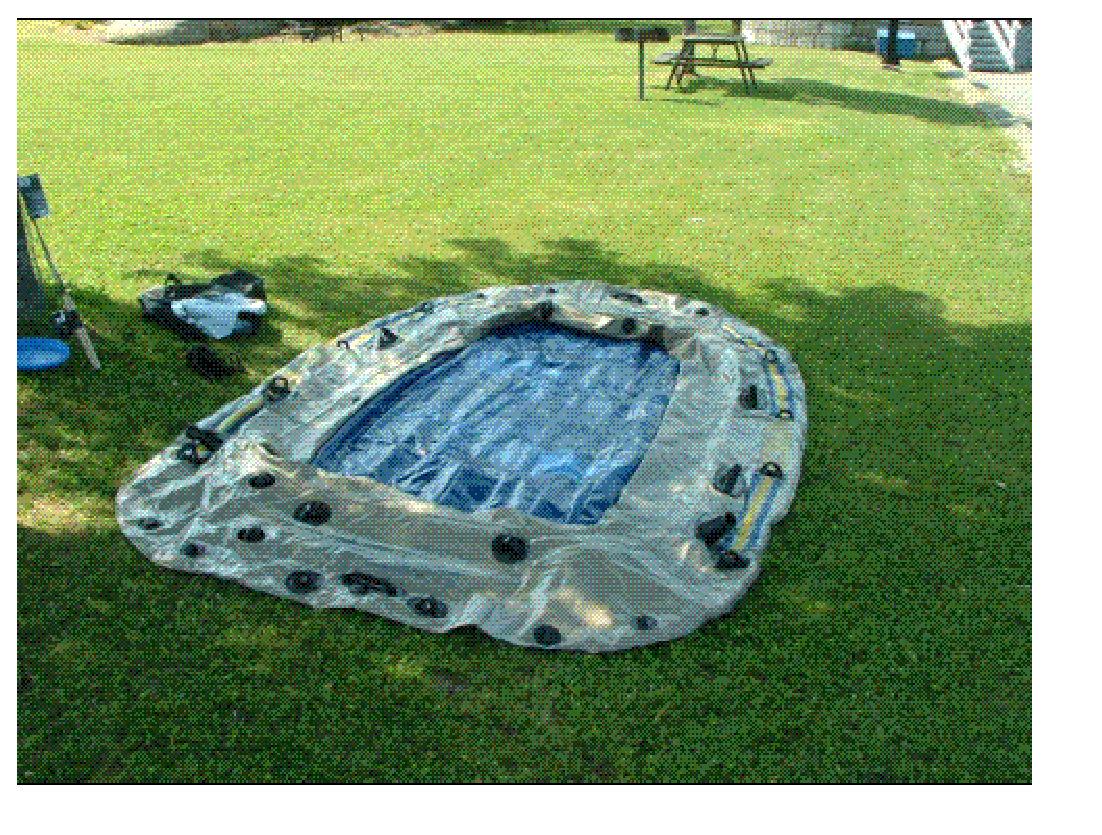
\epsfig{file=fig1.eps,width=3.5in}
Which one of the following is missing in it?
 
 
\noindent{\textbf{\large{
A.}}}
An airplane
 
 
\noindent{\textbf{\large{
B.}}}
An air-boat
 
 
\noindent{\textbf{\large{
C.}}}
Lawn
 
 
\noindent{\textbf{\large{
D.}}}
A table
 
 
\noindent{\textbf{\large{
E.}}}
A frisbee
 
 
\noindent{\textbf{\large{
F.}}}
  Not any of aboves.
 
 
\noindent\vspace{0.05in}{\textbf{\Large{Auto-answer:}}}
 
 
\noindent{\textbf{\large{
A.}}}
An airplane
 
 
\noindent\vspace{0.05in}{\textbf{\Large{End of auto-answer.}}}
 
 
 
\vspace{0.3in}
   
   
\noindent{\textbf{\Large{Total numbers: }}}
   
   
\noindent\begin{tabular}{|l|l|l|l|l|l|l|}
 \hline
Inputs & Calculates & Choices & Layers & Matches & Answer & Solution \\ \hline
           0  & 
           0  & 
           6
  simple  
  & 
           6  & 
           0  & 
  yes & 
  no 
  \\ \hline
 \end{tabular}
   
   
   
   
\noindent\vspace{0.1in}{\textbf{\Large{Calculated values:}}}
   
   
   
   
\noindent\vspace{0.1in}\hspace{-0.08in} {\textbf{\Large{All inputs: }}}
   
   
  
\vspace{0.2in}
  
{\textbf{\Large{Question
31.1.6 
 (           6 ,           6 ,          21 )
}}}
  
  
 
An object is subjected to an external net force $\mathbf{f}=(
60.0,  % 
5.0,
-6000.0  )N$. Its mass is known as
$m= % 
56.0 kg$. Please calculate its accelaration.
 
 
 
 
\noindent\vspace{0.05in}{\textbf{\Large{Answer:}}}
 
 

We will use the Newton's Second Law:
 
\[
\mathbf{f}=m\mathbf{a}.
\]
 
Since $\mathbf{f}=( % 
60.0,  % 
5.0,  % 
-6000.0 )N$
and $m= % 
56.0 kg$, bring them into the above equation, then we get
 
\begin{eqnarray*}
\mathbf{a}&=&\frac{\mathbf{f}}m  \\
&=&\frac{(
60.0 ,
5.0 ,
-6000.0 )N
}{ % 
56.0 kg}  \\
&=&(
1.0714 ,
8.9286 \times 10^{-2},
-107.14
)ms^{-2} \\
&=&(
13886. ,
1157.1 ,
-1.3886 \times 10^{6}
)km/h^2.
\end{eqnarray*}
 
 
 
\noindent\vspace{0.05in}{\textbf{\Large{End of Answer.}}}
 
 

 
 
 
\noindent\vspace{0.1in}{\textbf{\Large{Solution: }}}
 
 

We will use the Newton's Second Law:
 
\[
\mathbf{f}=m\mathbf{a}.
\]
 
Since $\mathbf{f}=( % 
60.0,  % 
5.0,  % 
-6000.0 )N$
and $m= % 
56.0 kg$, bring them into the above equation, then we get
 
\begin{eqnarray*}
\mathbf{a}&=&\frac{\mathbf{f}}m  \\
&=&\frac{(
60.0 ,
5.0 ,
-6000.0 )N
}{ % 
56.0 kg}  \\
&=&(
1.0714 ,
8.9286 \times 10^{-2},
-107.14
)ms^{-2} \\
&=&(
13886. ,
1157.1 ,
-1.3886 \times 10^{6}
)km/h^2.
\end{eqnarray*}
 
 
 
\noindent\vspace{0.1in}{\textbf{\Large{End of Solution.}}}
 
 

 
\vspace{0.3in}
   
   
\noindent{\textbf{\Large{Total numbers: }}}
   
   
\noindent\begin{tabular}{|l|l|l|l|l|l|l|}
 \hline
Inputs & Calculates & Choices & Layers & Matches & Answer & Solution \\ \hline
           4  & 
           6  & 
           0
  & 
           0  & 
           0  & 
  yes & 
  yes 
  \\ \hline
 \end{tabular}
   
   
   
   
\noindent\vspace{0.1in}{\textbf{\Large{Calculated values:}}}
   
   
  
  
\noindent\begin{tabular}{|l|l|l|l|}
\hline
 Sequential & Type & Accuracy & Calculated \\ 
\hline
 
 
  Calculated $            1 $ & real & $            5  $ & 
 $ 1.0714 $ 
 \\  \hline  
 
 
  Calculated $            2 $ & real & $            5  $ & 
 $ 8.9286 \times 10^{-2} $ 
 \\  \hline  
 
 
  Calculated $            3 $ & real & $            5  $ & 
 $ -107.14 $ 
 \\  \hline  
 
 
  Calculated $            4 $ & real & $            5  $ & 
 $ 13886. $ 
 \\  \hline  
 
 
  Calculated $            5 $ & real & $            5  $ & 
 $ 1157.1 $ 
 \\  \hline  
 
 
  Calculated $            6 $ & real & $            5  $ & 
 $ -1.3886 \times 10^{6} $ 
 \\  \hline  
 \end{tabular}
   
   
   
   
\noindent\vspace{0.1in}\hspace{-0.08in} {\textbf{\Large{All inputs: }}}
   
   
  
  
\noindent\begin{tabular}{|l|l|l|l|l|}
\hline
 Sequential & Type & Accuracy & Three inputs & Generated \\ 
\hline
 
 
  INPUT $            1 $ & real & $           -1  $ & $
 20.0
  $ & \\
  & & &  $
 101.0
  $ & \\
  & & &  $
 10.0
 $ & $ 60.0 $ 
 \\  \hline  
 
 
  INPUT $            2 $ & real & $           -1  $ & $
 2.0
  $ & \\
  & & &  $
 10.1
  $ & \\
  & & &  $
 1.0
 $ & $ 5.0 $ 
 \\  \hline  
 
 
  INPUT $            3 $ & real & $           -1  $ & $
 -2000.0
  $ & \\
  & & &  $
 -10001.0
  $ & \\
  & & &  $
 -1000.0
 $ & $ -6000.0 $ 
 \\  \hline  
 \end{tabular}
   
   
  
  
\noindent\begin{tabular}{|l|l|l|l|l|}
\hline
 Sequential & Type & Accuracy & Three inputs & Generated \\ 
\hline
 
 
  INPUT $            4 $ & real & $           -1  $ & $
 50.0
  $ & \\
  & & &  $
 60.1
  $ & \\
  & & &  $
 2.0
 $ & $ 56.0 $ 
 \\  \hline  
 \end{tabular}
   
   
   
   
\vspace{0.3in}
{\textbf{\LARGE{You have done all the above? A very good beginning, please go ahead.}}}
More constants the
Mass of electron
$m_e$$ =
9.109390 \times 10^{-31} $
kg
,
Universal gas constant
$R$$ =
8.315 $
J/(mol$\cdot $K)
,
$e$$ =
1.60217733 \times 10^{-19} $
C
, and
$m_p$$ =
1.6726231 \times 10^{-27} $
kg
%
may be very helpful.
\vspace{0.3in}
   
   
  
\vspace{0.2in}
  
{\textbf{\Large{QUESTION
31.2 
 (           3 ,           3 ,           3 )
}}}
  
  
Please choose the correct one from the following statements:
 
 
\noindent{\textbf{\large{
A.}}}
Canada has  %
35 provinces and  %
34 territories.
 
 
\noindent{\textbf{\large{
B.}}}
Canada has  %
37 provinces and  %
37 territories.
 
 
\noindent{\textbf{\large{
C.}}}
Canada has  %
34 provinces and  %
39 territories.
 
 
\noindent{\textbf{\large{
D.}}}
Canada has  %
33 provinces and  %
38 territories.
 
 
\noindent{\textbf{\large{
E.}}}
Canada has  %
36 provinces and  %
35 territories.
 
 
\noindent{\textbf{\large{
F.}}}
 None of above.
 
 
\noindent\vspace{0.05in}{\textbf{\Large{Auto-answer:}}}
 
 
\noindent{\textbf{\large{
F.}}}
 None of above.
 
 
\noindent\vspace{0.05in}{\textbf{\Large{End of auto-answer.}}}
 
 
   
   
\noindent{\textbf{\Large{Total numbers: }}}
   
   
\noindent\begin{tabular}{|l|l|l|l|l|l|l|}
 \hline
Inputs & Calculates & Choices & Layers & Matches & Answer & Solution \\ \hline
           0  & 
          20  & 
           6
  simple  
  & 
           6  & 
           0  & 
  yes & 
  no 
  \\ \hline
 \end{tabular}
   
   
   
   
\noindent\vspace{0.1in}{\textbf{\Large{Calculated values:}}}
   
   
  
  
\noindent\begin{tabular}{|l|l|l|l|}
\hline
 Sequential & Type & Accuracy & Calculated \\ 
\hline
 
 
  Calculated $            1 $ & integer &  & 
  $ 10 $ 
 \\  \hline  
 
 
  Calculated $            2 $ & integer &  & 
  $ 3 $ 
 \\  \hline  
 
 
  Calculated $            3 $ & integer &  & 
  $ 23 $ 
 \\  \hline  
 
 
  Calculated $            4 $ & integer &  & 
  $ 24 $ 
 \\  \hline  
 
 
  Calculated $            5 $ & integer &  & 
  $ 25 $ 
 \\  \hline  
 
 
  Calculated $            6 $ & integer &  & 
  $ 26 $ 
 \\  \hline  
 
 
  Calculated $            7 $ & integer &  & 
  $ 27 $ 
 \\  \hline  
 
 
  Calculated $            8 $ & integer &  & 
  $ 28 $ 
 \\  \hline  
 
 
  Calculated $            9 $ & integer &  & 
  $ 29 $ 
 \\  \hline  
 
 
  Calculated $           10 $ & integer &  & 
  $ 30 $ 
 \\  \hline  
 \end{tabular}
   
   
  
  
\noindent\begin{tabular}{|l|l|l|l|}
\hline
 Sequential & Type & Accuracy & Calculated \\ 
\hline
 
 
  Calculated $           11 $ & integer &  & 
  $ 31 $ 
 \\  \hline  
 
 
  Calculated $           12 $ & integer &  & 
  $ 32 $ 
 \\  \hline  
 
 
  Calculated $           13 $ & integer &  & 
  $ 33 $ 
 \\  \hline  
 
 
  Calculated $           14 $ & integer &  & 
  $ 34 $ 
 \\  \hline  
 
 
  Calculated $           15 $ & integer &  & 
  $ 35 $ 
 \\  \hline  
 
 
  Calculated $           16 $ & integer &  & 
  $ 36 $ 
 \\  \hline  
 
 
  Calculated $           17 $ & integer &  & 
  $ 37 $ 
 \\  \hline  
 
 
  Calculated $           18 $ & integer &  & 
  $ 38 $ 
 \\  \hline  
 
 
  Calculated $           19 $ & integer &  & 
  $ 39 $ 
 \\  \hline  
 
 
  Calculated $           20 $ & integer &  & 
  $ 40 $ 
 \\  \hline  
 \end{tabular}
   
   
   
   
\noindent\vspace{0.1in}\hspace{-0.08in} {\textbf{\Large{All inputs: }}}
   
   
  
\vspace{0.2in}
  
{\textbf{\Large{QUESTION
31.3 
 (           2 ,           2 ,           2 )
}}}
  
  
 
An object is subjected to an external net force $\mathbf{f}=(
80.000 ,
9.0000,
-5000.0  )N$. Its mass is known as
$m= % 
52.0000  kg$. Please choose the correct accelaration
from the following choices.
 
 
 
\noindent{\textbf{\large{
A.}}}
The accelaration is
$(
5.1859ms^{-2},
2243.1km/h^2,
-96.154ms^{-2}
).
$
 
 
\noindent{\textbf{\large{
B.}}}
The accelaration is
$(
5.1859ms^{-2},
4767.8km/h^2,
441.36ms^{-2}
).
$
 
 
\noindent{\textbf{\large{
C.}}}
The accelaration is
$(
1.5385ms^{-2},
2243.1km/h^2,
-96.154ms^{-2}
).
$
 
 
\noindent{\textbf{\large{
D.}}}
The accelaration is
$(
5.1859ms^{-2},
2243.1km/h^2,
441.36ms^{-2}
).
$
 
 
\noindent{\textbf{\large{
E.}}}
The accelaration is
$(
1.5385ms^{-2},
4767.8km/h^2,
-96.154ms^{-2}
).
$
 
 
\noindent{\textbf{\large{
F.}}}
The accelaration is
$(
1.5385ms^{-2},
2243.1km/h^2,
441.36ms^{-2}
).
$
 
 
\noindent{\textbf{\large{
G.}}}
 None of these.
 
 
\noindent\vspace{0.05in}{\textbf{\Large{Auto-answer:}}}
 
 
\noindent{\textbf{\large{
C.}}}
The accelaration is
$(
1.5385ms^{-2},
2243.1km/h^2,
-96.154ms^{-2}
).
$
 
 
\noindent\vspace{0.05in}{\textbf{\Large{End of auto-answer.}}}
 
 
 
 
 
 
\noindent\vspace{0.1in}{\textbf{\Large{Solution: }}}
 
 

We will use the Newton's Second Law:
 
\[
\mathbf{f}=m\mathbf{a}.
\]
 
Since $\mathbf{f}=( % 
80.000,  % 
9.0000,  % 
-5000.0 )N$
and $m= % 
52.0000kg$, bring them into the above equation, then we get
 
\begin{eqnarray*}
\mathbf{a}&=&\frac{\mathbf{f}}m  \\
&=&\frac{(
80.000 ,
9.0000 ,
-5000.0 )N
}{ % 
52.0000 kg}  \\
&=&(
1.5385 ,
0.17308,
-96.154
)ms^{-2} \\
&=&(
19938. ,
2243.1 ,
-1.2462 \times 10^{6}
)km/h^2.
\end{eqnarray*}
 
 
 
\noindent\vspace{0.1in}{\textbf{\Large{End of Solution.}}}
 
 

 
\vspace{0.3in}
   
   
\noindent{\textbf{\Large{Total numbers: }}}
   
   
\noindent\begin{tabular}{|l|l|l|l|l|l|l|}
 \hline
Inputs & Calculates & Choices & Layers & Matches & Answer & Solution \\ \hline
           4  & 
           6  & 
           7
  & 
           3  & 
           0  & 
  yes & 
  yes 
  \\ \hline
 \end{tabular}
   
   
   
   
\noindent\vspace{0.1in}{\textbf{\Large{Calculated values:}}}
   
   
  
  
\noindent\begin{tabular}{|l|l|l|l|}
\hline
 Sequential & Type & Accuracy & Calculated \\ 
\hline
 
 
  Calculated $            1 $ & real & $            5  $ & 
 $ 1.5385 $ 
 \\  \hline  
 
 
  Calculated $            2 $ & real & $            5  $ & 
 $ 0.17308 $ 
 \\  \hline  
 
 
  Calculated $            3 $ & real & $            5  $ & 
 $ -96.154 $ 
 \\  \hline  
 
 
  Calculated $            4 $ & real & $            5  $ & 
 $ 19938. $ 
 \\  \hline  
 
 
  Calculated $            5 $ & real & $            5  $ & 
 $ 2243.1 $ 
 \\  \hline  
 
 
  Calculated $            6 $ & real & $            5  $ & 
 $ -1.2462 \times 10^{6} $ 
 \\  \hline  
 \end{tabular}
   
   
   
   
\noindent\vspace{0.1in}\hspace{-0.08in} {\textbf{\Large{All inputs: }}}
   
   
  
  
\noindent\begin{tabular}{|l|l|l|l|l|}
\hline
 Sequential & Type & Accuracy & Three inputs & Generated \\ 
\hline
 
 
  INPUT $            1 $ & real & $           -3  $ & $
 20.000
  $ & \\
  & & &  $
 101.000
  $ & \\
  & & &  $
 10.000
 $ & $ 80.000 $ 
 \\  \hline  
 
 
  INPUT $            2 $ & real & $           -4  $ & $
 2.0000
  $ & \\
  & & &  $
 10.1000
  $ & \\
  & & &  $
 1.0000
 $ & $ 9.0000 $ 
 \\  \hline  
 
 
  INPUT $            3 $ & real & $           -1  $ & $
 -2000.0
  $ & \\
  & & &  $
 -10001.0
  $ & \\
  & & &  $
 -1000.0
 $ & $ -5000.0 $ 
 \\  \hline  
 \end{tabular}
   
   
  
  
\noindent\begin{tabular}{|l|l|l|l|l|}
\hline
 Sequential & Type & Accuracy & Three inputs & Generated \\ 
\hline
 
 
  INPUT $            4 $ & real & $           -4  $ & $
 50.0000
  $ & \\
  & & &  $
 60.1000
  $ & \\
  & & &  $
 2.0000
 $ & $ 52.0000 $ 
 \\  \hline  
 \end{tabular}
   
   
  
\vspace{0.2in}
  
{\textbf{\Large{QUESTION
31.4 
 (           4 ,           4 ,           4 )
}}}
  
  
Considering case-insensitivity, please match the following same strings.
  
  
\begin{tabular}{|l|l|l|}
 \hline
 Column Left & Column Right  & Your choinces \\ 
 \hline
{\textbf{\large{
A.}}}
B
  & 
YJH
 & 
 \\ 
 \hline
{\textbf{\large{
B.}}}
asdf(:)
  & 
 a= %
4
 & 
 \\ 
 \hline
{\textbf{\large{
C.}}}
 A= %
8/ %
2

  & 
c
 & 
 \\ 
 \hline
{\textbf{\large{
D.}}}
C
  & 
b
 & 
 \\ 
 \hline
{\textbf{\large{
E.}}}
yjh
  & 
ASDF(:)
 & 
 \\ 
 \hline
 \end{tabular}
  
  
 
 
\noindent\vspace{0.05in}{\textbf{\Large{Auto-answer:}}}
  
  
\begin{tabular}{|l|l|l|}
 \hline
 Column Left & Column Right  & Answers       \\ 
 \hline
{\textbf{\large{
A.}}}
B
  & 
YJH
 & 
{\textbf{\large{
E.}}}
 \\ 
 \hline
{\textbf{\large{
B.}}}
asdf(:)
  & 
 a= %
4
 & 
{\textbf{\large{
C.}}}
 \\ 
 \hline
{\textbf{\large{
C.}}}
 A= %
8/ %
2

  & 
c
 & 
{\textbf{\large{
D.}}}
 \\ 
 \hline
{\textbf{\large{
D.}}}
C
  & 
b
 & 
{\textbf{\large{
A.}}}
 \\ 
 \hline
{\textbf{\large{
E.}}}
yjh
  & 
ASDF(:)
 & 
{\textbf{\large{
B.}}}
 \\ 
 \hline
 \end{tabular}
  
  
 
 
\noindent\vspace{0.05in}{\textbf{\Large{End of auto-answer.}}}
 
 
 
   
   
\noindent{\textbf{\Large{Total numbers: }}}
   
   
\noindent\begin{tabular}{|l|l|l|l|l|l|l|}
 \hline
Inputs & Calculates & Choices & Layers & Matches & Answer & Solution \\ \hline
           2  & 
           1  & 
           0
  & 
          16  & 
           5  & 
  yes & 
  no 
  \\ \hline
 \end{tabular}
   
   
   
   
\noindent\vspace{0.1in}{\textbf{\Large{Calculated values:}}}
   
   
  
  
\noindent\begin{tabular}{|l|l|l|l|}
\hline
 Sequential & Type & Accuracy & Calculated \\ 
\hline
 
 
  Calculated $            1 $ & integer &  & 
  $ 4 $ 
 \\  \hline  
 \end{tabular}
   
   
   
   
\noindent\vspace{0.1in}\hspace{-0.08in} {\textbf{\Large{All inputs: }}}
   
   
  
  
\noindent\begin{tabular}{|l|l|l|l|l|}
\hline
 Sequential & Type & Accuracy & Three inputs & Generated \\ 
\hline
 
 
  INPUT $            1 $ & integer &  & $
 2
 , 
 8
 , 
 2
 $ & $ 8 $ 
 \\  \hline  
 
 
  INPUT $            2 $ & integer &  & $
 2
 , 
 3
 , 
 2
 $ & $ 2 $ 
 \\  \hline  
 \end{tabular}
   
   
  
\vspace{0.2in}
  
{\textbf{\Large{QUESTION
31.5 
 (           5 ,           5 ,           5 )
}}}
  
  
If any one of the following statements is correct, please fill the box ahead of it with $T$ .
If wrong, fill with $F$.
 
\noindent\begin{tabular}{|l|l|}\hline Your&\hspace{.2in} \\ answer&\hspace{.2in} \\ \hline \end{tabular}
1. $ % 
50$ is an  % 
even number.
 
\noindent\begin{tabular}{|l|l|}\hline Your&\hspace{.2in} \\ answer&\hspace{.2in} \\ \hline \end{tabular}
2.  % 
Montreal is in  % 
Ontario province.
 
\noindent\begin{tabular}{|l|l|}\hline Your&\hspace{.2in} \\ answer&\hspace{.2in} \\ \hline \end{tabular}
3.  % 
$\mathbf{F}=m\mathbf{a}$ is a mathmatical form of
the Newton's Second Law.
 
 
 
\noindent\vspace{0.05in}{\textbf{\Large{Answer:}}}
 
 

 
\noindent\begin{tabular}{|l|l|}\hline The correct & \\
          answer &  % 
$T$ \\ \hline \end{tabular}
1. $ % 
50$ is an  % 
even number.
 
\noindent\begin{tabular}{|l|l|}\hline The correct & \\
          answer &  % 
$F$ \\ \hline \end{tabular}
2.  % 
Montreal is in  % 
Ontario province.
 
\noindent\begin{tabular}{|l|l|}\hline The correct & \\
          answer &  % 
$T$ \\ \hline \end{tabular}
3.  % 
$\mathbf{F}=m\mathbf{a}$ is a mathmatical form of  % 
the Newton's Second Law.
 
 
 
\noindent\vspace{0.05in}{\textbf{\Large{End of Answer.}}}
 
 

 
\vspace{0.3in}
   
   
\noindent{\textbf{\Large{Total numbers: }}}
   
   
\noindent\begin{tabular}{|l|l|l|l|l|l|l|}
 \hline
Inputs & Calculates & Choices & Layers & Matches & Answer & Solution \\ \hline
           6  & 
           3  & 
           0
  & 
           0  & 
           0  & 
  yes & 
  no 
  \\ \hline
 \end{tabular}
   
   
   
   
\noindent\vspace{0.1in}{\textbf{\Large{Calculated values:}}}
   
   
  
  
\noindent\begin{tabular}{|l|l|l|l|}
\hline
 Sequential & Type & Accuracy & Calculated \\ 
\hline
 
 
  Calculated $            1 $ & string & $            1  $ ( $           1  $ strings): 
 & $T$
 \\  \hline  
 
 
  Calculated $            2 $ & string & $            1  $ ( $           1  $ strings): 
 & $F$
 \\  \hline  
 
 
  Calculated $            3 $ & string & $            1  $ ( $           1  $ strings): 
 & $T$
 \\  \hline  
 \end{tabular}
   
   
   
   
\noindent\vspace{0.1in}\hspace{-0.08in} {\textbf{\Large{All inputs: }}}
   
   
  
  
\noindent\begin{tabular}{|l|l|l|l|l|}
\hline
 Sequential & Type & Accuracy & Three inputs & Generated \\ 
\hline
 
 
  INPUT $            1 $ & integer &  & $
 1
 , 
 100
 , 
 1
 $ & $ 50 $ 
 \\  \hline  
 
 
  INPUT $            2 $ & string & & 
 even & 
  $ <-- $ 
  \\
  & & & 
 odd & 
 \\  \hline  
 
 
  INPUT $            3 $ & string & & 
 Toronto & 
  \\
  & & & 
 Kingston & 
  \\
  & & & 
 Montreal & 
  $ <-- $ 
  \\
  & & & 
 Hull & 
 \\  \hline  
 \end{tabular}
   
   
  
  
\noindent\begin{tabular}{|l|l|l|l|l|}
\hline
 Sequential & Type & Accuracy & Three inputs & Generated \\ 
\hline
 
 
  INPUT $            4 $ & string & & 
 Ontario & 
  $ <-- $ 
  \\
  & & & 
 Quebec & 
 \\  \hline  
 
 
  INPUT $            5 $ & string & & 
 $\mathbf{F}=m\mathbf{a}$ & 
  $ <-- $ 
  \\
  & & & 
 $\left| \mathbf{F}\right| =Gm_1m_2r^{-2}$ & 
 \\  \hline  
 
 
  INPUT $            6 $ & string & & 
 the Newton's Second Law & 
  $ <-- $ 
  \\
  & & & 
 Newton's Law of Universal Gravitation & 
 \\  \hline  
 \end{tabular}
   
   
  
\vspace{0.2in}
  
{\textbf{\Large{QUESTION
31.6 
 (           1 ,           1 ,           1 )
}}}
  
  


\noindent\vspace{0.05in}{\textbf{\Large{Abstract:}}}
This is a simple Newton's Second Law calculation multi-choice problem.  
\noindent\vspace{0.05in}{\textbf{\Large{end of abstract.}}}


 
 
An object is subjected to an external net force $\mathbf{f}=
(40.0 , 3.0 , -6000.0) N$.
Its mass is known as $m= % 
52.0000 kg$. Please choose the
correct accelaration from the following choices.
 
 
 
\noindent{\textbf{\large{
A.}}}
The accelaration is $  %
(
-1.89,
0.26,
-115.38)
ms^{-2} $.
 
 
\noindent{\textbf{\large{
B.}}}
The accelaration is $  %
(
0.769,
5.8 \times 10^{-2},
-115.38)
ms^{-2} $.
 
 
\noindent{\textbf{\large{
C.}}}
The accelaration is $  %
(
-1.89,
5.8 \times 10^{-2},
-115.38)
ms^{-2} $.
 
 
\noindent{\textbf{\large{
D.}}}
The accelaration is $  %
(
-1.89,
0.26,
-412.14)
ms^{-2} $.
 
 
\noindent{\textbf{\large{
E.}}}
The accelaration is $  %
(
0.769,
0.26,
-115.38)
ms^{-2} $.
 
 
\noindent{\textbf{\large{
F.}}}
The accelaration is $  %
(
0.769,
0.26,
-412.14)
ms^{-2} $.
 
 
\noindent{\textbf{\large{
G.}}}
The accelaration is $  %
(
0.769,
5.8 \times 10^{-2},
-412.14)
ms^{-2} $.
 
 
\noindent{\textbf{\large{
H.}}}
The accelaration is $  %
(
-1.89,
5.8 \times 10^{-2},
-412.14)
ms^{-2} $.
 
 
\noindent\vspace{0.05in}{\textbf{\Large{Auto-answer:}}}
 
 
\noindent{\textbf{\large{
B.}}}
The accelaration is $  %
(
0.769,
5.8 \times 10^{-2},
-115.38)
ms^{-2} $.
 
 
\noindent\vspace{0.05in}{\textbf{\Large{End of auto-answer.}}}
 
 
 
 
 
\noindent\vspace{0.05in}{\textbf{\Large{Answer:}}}
 
 

The correct answer from the choices is


\noindent{\textbf{\large{
B.}}}
The accelaration is $  %
(
0.769,
5.8 \times 10^{-2},
-115.38)
ms^{-2} $.
 
 
 
\noindent\vspace{0.05in}{\textbf{\Large{End of Answer.}}}
 
 

 
 
 
\noindent\vspace{0.1in}{\textbf{\Large{Solution: }}}
 
 

We will use the Newton's Second Law:
 
\[
\mathbf{f}=m\mathbf{a}.
\]
 
Since $\mathbf{f}= % 
(40.0 , 3.0 , -6000.0) N$
and $m= % 
52.0000kg$, bring them into the above equation, then we get
 
\begin{eqnarray*}
\mathbf{a}&=&\frac{\mathbf{f}}m  \\
&=&\frac{ % 
(40.0 , 3.0 , -6000.0) N}{ % 
52.0000kg}  \\
&=& % 
(0.769 , 5.8 \times 10^{-2} , -115.38) ms^{-2}
\end{eqnarray*}
 
 
 
\noindent\vspace{0.1in}{\textbf{\Large{End of Solution.}}}
 
 

 
\vspace{0.3in}
   
   
\noindent{\textbf{\Large{Total numbers: }}}
   
   
\noindent\begin{tabular}{|l|l|l|l|l|l|l|}
 \hline
Inputs & Calculates & Choices & Layers & Matches & Answer & Solution \\ \hline
           2  & 
           1  & 
           8
  & 
           3  & 
           0  & 
  yes & 
  yes 
  \\ \hline
 \end{tabular}
   
   
   
   
\noindent\vspace{0.1in}{\textbf{\Large{Calculated values:}}}
   
   
  
  
\noindent\begin{tabular}{|l|l|l|l|}
\hline
 Sequential & Type & Accuracy & Calculated \\ 
\hline
 
 
  Calculated $            1 $ & vector &  
  $            3  $ 
 &  $ 0.769 $ 
 \\    
  & & 
  $            2  $ 
 &  $ 5.8 \times 10^{-2} $ 
 \\    
  & & 
  $            5  $ 
 &  $ -115.38 $ 
 \\  \hline  
 \end{tabular}
   
   
   
   
\noindent\vspace{0.1in}\hspace{-0.08in} {\textbf{\Large{All inputs: }}}
   
   
  
  
\noindent\begin{tabular}{|l|l|l|l|l|}
\hline
 Sequential & Type & Accuracy & Three inputs & Generated \\ 
\hline
 
 
  INPUT $            1 $ & vector & $           -1  $ & $
20.0
  $ & \\
  & & & $
101.0
  $ & \\
  & & & $
10.0
$ & $ 40.0 $ 
  \\
  & & $           -1  $ & $
2.0
  $ & \\
  & & & $
10.1
  $ & \\
  & & & $
1.0
$ & $ 3.0 $ 
  \\
  & & $           -1  $ & $
-2000.0
  $ & \\
  & & & $
-10001.0
  $ & \\
  & & & $
-1000.0
$ & $ -6000.0 $ 
 \\  \hline  
 
 
  INPUT $            2 $ & real & $           -4  $ & $
 50.0000
  $ & \\
  & & &  $
 60.1000
  $ & \\
  & & &  $
 2.0000
 $ & $ 52.0000 $ 
 \\  \hline  
 \end{tabular}
   
   
   
   
\vspace{0.3in}
{\textbf{\LARGE{You have done all the above? Excellent! Not much left, please continue.}}}
\vspace{0.3in}
   
   
  
\vspace{0.2in}
  
{\textbf{\Large{QUESTION
31.7 
 (           8 ,          15 ,          60 )
}}}
  
  
 
$ \left( \begin{array}{ccccccccc}
           5  & 
           6  & 
           6  & 
           6  \\ 
           6  & 
           4  & 
           4  & 
           4  \\ 
           5  & 
           6  & 
           5  & 
           5
\end{array}\right) \times
\left( \begin{array}{c}
           2  \\ 
           2  \\ 
           2  \\ 
           2
\end{array}\right) $ =?
 
 
$  % 
 \left( \begin{array}
 {
 c
 c
 }
 \Theta & 
 \delta \\ 
                    \Xi & 
 \varepsilon \\ 
 \delta & 
 \beta \\ 
 \Phi & 
                    \Xi
 \end{array} \right)
 \left( \begin{array}
 {
 c
 }
 \gamma \\ 
 \beta
 \end{array} \right)
$ =?
 
 
 
\noindent\vspace{0.05in}{\textbf{\Large{Answer:}}}
 
 

 
$\left( \begin{array}{ccccccccccccccc}
           5  & 
           6  & 
           6  & 
           6  \\ 
           6  & 
           4  & 
           4  & 
           4  \\ 
           5  & 
           6  & 
           5  & 
           5
\end{array}\right) \times
\left( \begin{array}{c}
           2  \\ 
           2  \\ 
           2  \\ 
           2
\end{array}\right)  =
\left( \begin{array}{c}
          46  \\ 
          36  \\ 
          42
\end{array}\right)  $
 
$  % 
 \left( \begin{array}
 {
 c
 c
 }
 \Theta & 
 \delta \\ 
                    \Xi & 
 \varepsilon \\ 
 \delta & 
 \beta \\ 
 \Phi & 
                    \Xi
 \end{array} \right)
 \left( \begin{array}
 {
 c
 }
 \gamma \\ 
 \beta
 \end{array} \right)
=
 \left( \begin{array}
 {
 c
 }
  \Theta \times  \gamma +  \delta \times  \beta \\ 
                     \Xi \times  \gamma +  \varepsilon \times  \beta \\ 
  \delta \times  \gamma +  \beta \times  \beta \\ 
  \Phi \times  \gamma +                     \Xi \times  \beta
 \end{array} \right)
$
 
 
 
\noindent\vspace{0.05in}{\textbf{\Large{End of Answer.}}}
 
 

 
 
 
\noindent\vspace{0.1in}{\textbf{\Large{Solution: }}}
 
 

 
 
\noindent\vspace{0.1in}{\textbf{\Large{End of Solution.}}}
 
 

 
\vspace{0.3in}
   
   
\noindent{\textbf{\Large{Total numbers: }}}
   
   
\noindent\begin{tabular}{|l|l|l|l|l|l|l|}
 \hline
Inputs & Calculates & Choices & Layers & Matches & Answer & Solution \\ \hline
           4  & 
           2  & 
           0
  & 
           0  & 
           0  & 
  yes & 
  yes 
  \\ \hline
 \end{tabular}
   
   
   
   
\noindent\vspace{0.1in}{\textbf{\Large{Calculated values:}}}
   
   
  
  
\noindent\begin{tabular}{|l|l|l|l|}
\hline
 Sequential & Type & Accuracy & Calculated \\ 
\hline
 
 
  Calculated $            1 $ & i-matrix &  & 
 (size:            3  by            1 )
 \\  \hline  
 \end{tabular}
   
   
$\begin{array}{
 c
 }
          46  \\ 
          36  \\ 
          42
 \end{array}  $ 
  
  
\noindent\begin{tabular}{|l|l|l|l|}
\hline
 Sequential & Type & Accuracy & Calculated \\ 
\hline
 
 
  Calculated $            2 $ & s-matrix & & 
 (size:            4  by            1 )
 \\  \hline  
 \end{tabular}
   
   
 $  \left( \begin{array}
 {
 c
 }
  \Theta \times  \gamma +  \delta \times  \beta \\ 
                     \Xi \times  \gamma +  \varepsilon \times  \beta \\ 
  \delta \times  \gamma +  \beta \times  \beta \\ 
  \Phi \times  \gamma +                     \Xi \times  \beta
 \end{array} \right) $ 
   
   
\noindent\vspace{0.1in}\hspace{-0.08in} {\textbf{\Large{All inputs: }}}
   
   
  
  
\noindent\begin{tabular}{|l|l|l|l|l|}
\hline
 Sequential & Type & Accuracy & Three inputs & Generated \\ 
\hline
 
 
  INPUT $            1 $ & i-matrix &  & $
 4
 , 
 7
 , 
 1
 $ & (size:            3  by            4 )
 \\  \hline  
 \end{tabular}
   
   
 $\begin{array}{
 c
 c
 c
 c
 }
           5  & 
           6  & 
           6  & 
           6  \\ 
           6  & 
           4  & 
           4  & 
           4  \\ 
           5  & 
           6  & 
           5  & 
           5
\end{array}  $ 
  
  
\noindent\begin{tabular}{|l|l|l|l|l|}
\hline
 Sequential & Type & Accuracy & Three inputs & Generated \\ 
\hline
 
 
  INPUT $            2 $ & i-matrix &  & $
 2
 , 
 2
 , 
 1
 $ & (size:            4  by            1 )
 \\  \hline  
 \end{tabular}
   
   
 $\begin{array}{
 c
 }
           2  \\ 
           2  \\ 
           2  \\ 
           2
\end{array}  $ 
  
  
\noindent\begin{tabular}{|l|l|l|l|l|}
\hline
 Sequential & Type & Accuracy & Three inputs & Generated \\ 
\hline
 
 
  INPUT $            3 $ & s-matrix & & 
 $  \alpha $ & 
  \\
  & & & 
 $  \beta $ & 
  \\
  & & & 
 $  \gamma $ & 
  \\
  & & & 
 $  \delta $ & 
  \\
  & & & 
 $  \epsilon $ & 
  \\
  & & & 
 $  \varepsilon $ & 
  \\
  & & & 
 $                     \zeta $ & 
  \\
  & & & 
 $  \eta $ & 
  \\
  & & & 
 $  \rho $ & 
  \\
  & & & 
 $  \sigma $ & 
  \\
  & & & 
 $  \Gamma $ & 
  \\
  & & & 
 $  \Delta $ & 
  \\
  & & & 
 $  \Theta $ & 
  \\
  & & & 
 $  \Lambda $ & 
  \\
  & & & 
 $                     \Xi $ & 
  \\
  & & & 
 $  \Upsilon $ & 
  \\
  & & & 
 $  \Phi $ & 
  \\
  & & & 
 $  \Psi $ & 
  \\
  & & & 
 $  \Omega $ & 
  (size:            4  by            2 )
 \\  \hline  
 \end{tabular}
   
   
 $  \left( \begin{array}
 {
 c
 c
 }
 \Theta & 
 \delta \\ 
                    \Xi & 
 \varepsilon \\ 
 \delta & 
 \beta \\ 
 \Phi & 
                    \Xi
 \end{array} \right) $ 
  
  
\noindent\begin{tabular}{|l|l|l|l|l|}
\hline
 Sequential & Type & Accuracy & Three inputs & Generated \\ 
\hline
 
 
  INPUT $            4 $ & s-matrix & & 
 $  \beta $ & 
  \\
  & & & 
 $  \gamma $ & 
  (size:            2  by            1 )
 \\  \hline  
 \end{tabular}
   
   
 $  \left( \begin{array}
 {
 c
 }
 \gamma \\ 
 \beta
 \end{array} \right) $ 
  
\vspace{0.2in}
  
{\textbf{\Large{QUESTION
31.8 
 (           7 ,          14 ,          50 )
}}}
  
  
 
An object is subjected to an external net force $\mathbf{f}=
(90.0 , 5.0 , -3000.0) N$.
Its mass is known as $m= % 
52.0 kg$.
Please choose the correct accelaration from the following choices.
 
 
\noindent{\textbf{\large{
A.}}}
  The accelaration is $  %
(
1.73,
9.6 \times 10^{-2},
254.30)
ms^{-2} $.
 
 
\noindent{\textbf{\large{
B.}}}
  The accelaration is $  %
(
-5.03,
9.6 \times 10^{-2},
254.30)
ms^{-2} $.
 
 
\noindent{\textbf{\large{
C.}}}
  The accelaration is $  %
(
1.73,
9.6 \times 10^{-2},
-57.692)
ms^{-2} $.
 
 
\noindent{\textbf{\large{
D.}}}
  The accelaration is $  %
(
1.73,
0.33,
254.30)
ms^{-2} $.
 
 
\noindent\vspace{0.05in}{\textbf{\Large{Auto-answer:}}}
 
 
\noindent{\textbf{\large{
C.}}}
  The accelaration is $  %
(
1.73,
9.6 \times 10^{-2},
-57.692)
ms^{-2} $.
 
 
\noindent\vspace{0.05in}{\textbf{\Large{End of auto-answer.}}}
 
 
 
 
 
\noindent\vspace{0.1in}{\textbf{\Large{Solution: }}}
 
 

We will use the Newton's Second Law:
 
\[
\mathbf{f}=m\mathbf{a}.
\]
 
Since $\mathbf{f}= % 
(90.0 , 5.0 , -3000.0) N$
and $m= % 
52.0kg$, bring them into the above equation, then we get
 
\begin{eqnarray*}
\mathbf{a}&=&\frac{\mathbf{f}}m  \\
&=&\frac{ % 
(90.0 , 5.0 , -3000.0) N}{ % 
52.0kg}  \\
&=& % 
(1.73 , 9.6 \times 10^{-2} , -57.692) ms^{-2}
\end{eqnarray*}
 
 
 
\noindent\vspace{0.1in}{\textbf{\Large{End of Solution.}}}
 
 

 
 
\vspace{0.3in}
   
   
\noindent{\textbf{\Large{Total numbers: }}}
   
   
\noindent\begin{tabular}{|l|l|l|l|l|l|l|}
 \hline
Inputs & Calculates & Choices & Layers & Matches & Answer & Solution \\ \hline
           2  & 
           1  & 
           4
  & 
           3  & 
           0  & 
  yes & 
  yes 
  \\ \hline
 \end{tabular}
   
   
   
   
\noindent\vspace{0.1in}{\textbf{\Large{Calculated values:}}}
   
   
  
  
\noindent\begin{tabular}{|l|l|l|l|}
\hline
 Sequential & Type & Accuracy & Calculated \\ 
\hline
 
 
  Calculated $            1 $ & vector &  
  $            3  $ 
 &  $ 1.73 $ 
 \\    
  & & 
  $            2  $ 
 &  $ 9.6 \times 10^{-2} $ 
 \\    
  & & 
  $            5  $ 
 &  $ -57.692 $ 
 \\  \hline  
 \end{tabular}
   
   
   
   
\noindent\vspace{0.1in}\hspace{-0.08in} {\textbf{\Large{All inputs: }}}
   
   
  
  
\noindent\begin{tabular}{|l|l|l|l|l|}
\hline
 Sequential & Type & Accuracy & Three inputs & Generated \\ 
\hline
 
 
  INPUT $            1 $ & vector & $           -1  $ & $
20.0
  $ & \\
  & & & $
101.0
  $ & \\
  & & & $
10.0
$ & $ 90.0 $ 
  \\
  & & $           -1  $ & $
2.0
  $ & \\
  & & & $
10.1
  $ & \\
  & & & $
1.0
$ & $ 5.0 $ 
  \\
  & & $           -1  $ & $
-2000.0
  $ & \\
  & & & $
-10001.0
  $ & \\
  & & & $
-1000.0
$ & $ -3000.0 $ 
 \\  \hline  
 
 
  INPUT $            2 $ & real & $           -1  $ & $
 50.0
  $ & \\
  & & &  $
 60.1
  $ & \\
  & & &  $
 2.0
 $ & $ 52.0 $ 
 \\  \hline  
 \end{tabular}
   
   
  
\vspace{0.2in}
  
{\textbf{\Large{QUESTION
31.9 
 (           9 ,          16 ,          70 )
}}}
  
  


\noindent\vspace{0.05in}{\textbf{\Large{Abstract:}}}
Quadratic Equation constructed from the following first two random (input) integers as roots,  
which of course should not show in the exam papers.  
\noindent\vspace{0.05in}{\textbf{\Large{end of abstract.}}}


 
 
% First root
% Second root

 
Please solve the following equation:
\begin{eqnarray*}
3 \times x^2  % 
-162
                 \times x    % 
+  % 
1599 =0
\end{eqnarray*}
 
 
 
\noindent\vspace{0.05in}{\textbf{\Large{Answer:}}}
 
 

13,  % 
41
 
 
 
\noindent\vspace{0.05in}{\textbf{\Large{End of Answer.}}}
 
 

 
 
 
\noindent\vspace{0.1in}{\textbf{\Large{Solution: }}}
 
 

Roots to the equation
\begin{eqnarray*}
3 \times x^2  % 
-162
                 \times x    % 
+  % 
1599 =0
\end{eqnarray*}
are  % 
13 and  % 
41 .
 
Let us verity  % 
13 first:
$  % 
3 \times x^2  % 
-162
                 \times x    % 
+  % 
1599
  = % 
507+( % 
-2106)+( % 
1599)
  = % 
-1599+( % 
1599)
  = % 
0
$
 
Then verity  % 
41:
$  % 
3 \times x^2  % 
-162
                 \times x    % 
+  % 
1599
  = % 
5043+( % 
-6642)+( % 
1599)
  = % 
-1599+( % 
1599)
  = % 
0
$
 
 
 
\noindent\vspace{0.1in}{\textbf{\Large{End of Solution.}}}
 
 

 
\vspace{0.3in}
   
   
\noindent{\textbf{\Large{Total numbers: }}}
   
   
\noindent\begin{tabular}{|l|l|l|l|l|l|l|}
 \hline
Inputs & Calculates & Choices & Layers & Matches & Answer & Solution \\ \hline
           3  & 
          13  & 
           0
  & 
           0  & 
           0  & 
  yes & 
  yes 
  \\ \hline
 \end{tabular}
   
   
   
   
\noindent\vspace{0.1in}{\textbf{\Large{Calculated values:}}}
   
   
  
  
\noindent\begin{tabular}{|l|l|l|l|}
\hline
 Sequential & Type & Accuracy & Calculated \\ 
\hline
 
 
  Calculated $            1 $ & integer &  & 
  $ 3 $ 
 \\  \hline  
 
 
  Calculated $            2 $ & string & $            1  $ ( $           1  $ strings): 
 & 
 \\  \hline  
 
 
  Calculated $            3 $ & integer &  & 
  $ -162 $ 
 \\  \hline  
 
 
  Calculated $            4 $ & string & $            1  $ ( $           1  $ strings): 
 & +
 \\  \hline  
 
 
  Calculated $            5 $ & integer &  & 
  $ 1599 $ 
 \\  \hline  
 
 
  Calculated $            6 $ & integer &  & 
  $ 507 $ 
 \\  \hline  
 
 
  Calculated $            7 $ & integer &  & 
  $ -2106 $ 
 \\  \hline  
 
 
  Calculated $            8 $ & integer &  & 
  $ -1599 $ 
 \\  \hline  
 
 
  Calculated $            9 $ & integer &  & 
  $ 0 $ 
 \\  \hline  
 
 
  Calculated $           10 $ & integer &  & 
  $ 5043 $ 
 \\  \hline  
 \end{tabular}
   
   
  
  
\noindent\begin{tabular}{|l|l|l|l|}
\hline
 Sequential & Type & Accuracy & Calculated \\ 
\hline
 
 
  Calculated $           11 $ & integer &  & 
  $ -6642 $ 
 \\  \hline  
 
 
  Calculated $           12 $ & integer &  & 
  $ -1599 $ 
 \\  \hline  
 
 
  Calculated $           13 $ & integer &  & 
  $ 0 $ 
 \\  \hline  
 \end{tabular}
   
   
   
   
\noindent\vspace{0.1in}\hspace{-0.08in} {\textbf{\Large{All inputs: }}}
   
   
  
  
\noindent\begin{tabular}{|l|l|l|l|l|}
\hline
 Sequential & Type & Accuracy & Three inputs & Generated \\ 
\hline
 
 
  INPUT $            1 $ & integer &  & $
 -11
 , 
 30
 , 
 4
 $ & $ 13 $ 
 \\  \hline  
 
 
  INPUT $            2 $ & integer &  & $
 -31
 , 
 60
 , 
 3
 $ & $ 41 $ 
 \\  \hline  
 
 
  INPUT $            3 $ & integer &  & $
 -15
 , 
 15
 , 
 2
 $ & $ 3 $ 
 \\  \hline  
 \end{tabular}
   
   
   
   
   
   
 \vspace{0.2in}
Here are still some constants for use:
 
 
\noindent\begin{tabular}{|l|l|l|}
\hline
Constant & Symbol & Value \\
\hline
 
Mass of proton &
$m_p$ &
 $ 1.6726231 \times 10^{-27} $
kg \\
\hline
 
Boltzmann's constant &
$k$ &
 $ 1.381 \times 10^{-23} $
J/K \\
\hline
 
\end{tabular}
 
Thank you very much for answering these questions!
 
{\textbf{\large{Please be advised}}} that in this paper there are questions from
31.1 through
31.9.
And any one of them may contain more than one sub-question, thus the total number
of sub-questions here is around 14, of which
13 should be answered.
 
   
   
\vspace{2.0in} PAPER TAIL GENERATED.
   
   
   
   
\vspace{1.0in} 
{\textbf{\large{ *** END OF PAPER, THANKS *** }}} 
   
   
\hspace{1.0in} By: 
         239 (          26 ,           34 )
   
   
   
   
\newpage 
\setcounter{page}{ 
    32001 } 
   
   
\noindent{\textbf{\huge{THIS IS THE JOURNAL FOR}}}
   
   
 {\textbf{ \Large{ PAPER NUMBER           32  }}}
   
   
\vspace{0.2in}
   
   
\markboth{Journal NOT for examinees !!! {\today}}{Journal NOT for examinees !!! {\today}}
   
   
   
   
   
   
 \vspace{0.2in}
 
 
{\Huge  THIS IS AN EXAMPLE OF}
 
{\Huge  PERSONALIZED TESTS. }
 
If needed, please use the following constants.
 
 
 
\noindent\begin{tabular}{|l|l|l|}
\hline
Constant & Symbol & Value \\
\hline
Acceleration due to earth's gravity &
$g$ &
 $ 9.80 $
m/s$^2$ \\
\hline
Avogadro's number &
$N_A$ &
 $ 6.0221367 \times 10^{23} $
mol$^{-1}$ \\
\hline
Boltzmann's constant &
$k$ &
 $ 1.380658 \times 10^{-23} $
J/K \\
\hline
Coulomb's constant &
$k$ &
 $ 8.99 \times 10^{9} $
N$\cdot $m$^2$/C$^2$ \\
\hline
Electron charge magnitiude &
$e$ &
 $ 1.60217733 \times 10^{-19} $
C \\
\hline
Permeability of free space &
$\mu _0$ &
 $ 1.25663706 \times 10^{-6} $
T$\cdot $m/A \\
\hline
Permittivity of free space &
$\epsilon _0$ &
 $ 8.854187817 \times 10^{-12} $
C$^2$/(N$\cdot $m$^2$) \\
\hline
Pi &
$\pi$ &
 $ 3.14159265 $
$ $ \\
\hline
Planck's constant &
$h$ &
 $ 6.6260755 \times 10^{-34} $
J$\cdot $s \\
\hline
Mass of electron &
$m_e$ &
 $ 9.1093897 \times 10^{-31} $
kg \\
\hline
\end{tabular}
 
 
\noindent\begin{tabular}{|l|l|l|}
\hline
Constant & Symbol & Value \\
\hline
Mass of neutron &
$m_n$ &
 $ 1.6749286 \times 10^{-27} $
kg \\
\hline
Mass of proton &
$m_p$ &
 $ 1.6726231 \times 10^{-27} $
kg \\
\hline
Speed of light in vacuum &
$c$ &
 $ 299792458. $
m/s \\
\hline
Universal gravitational constant &
$G$ &
 $ 6.67259 \times 10^{-11} $
N$\cdot $m$^2$/kg$^2$ \\
\hline
Universal gas constant &
$R$ &
 $ 8.314510 $
J/(mol$\cdot $K) \\
\hline
\end{tabular}
 
 
{\textbf{\large{Please be advised}}} that in this paper there are questions from
32.1 through
32.9.
And any one of them may contain more than one sub-question, thus the total number
of sub-questions here is around 14, of which
13 should be answered.
 
\vspace{0.3in}
 
 
   
   
 PAPER TITLE GENERATED.
   
   
   
\vspace{0.2in}
   
In this paper, big questions will be generated in the following order: 
   
   
             1 (           6 )
 ,
             2 (           5 )
 ,
             3 (           3 )
 ,
             4 (           2 )
 ,
             5 (           4 )
 ,
             6 (           1 )
 ,
             7 (           8 )
 ,
             8 (           7 )
 ,
             9 (           9 )
 .
  
\vspace{0.2in}
  
{\textbf{\Large{QUESTION
32.1 
 (           6 )
}}}
  
  
 
{\textbf{\Large{Please answer ONLY
5 of the following
6 questions (Questions
32.1.1 through
32.1.6). }}}
 
Here are still some constants for use in the following questions:
 
 
\noindent\begin{tabular}{|l|l|l|}
\hline
Constant & Symbol & Value \\
\hline
 
Boltzmann's constant &
$k$ &
 $ 1.381 \times 10^{-23} $
J/K \\
\hline
 
Avogadro's number &
$N_A$ &
 $ 6.022 \times 10^{23} $
mol$^{-1}$ \\
\hline
 
Mass of electron &
$m_e$ &
 $ 9.1093897 \times 10^{-31} $
kg \\
\hline
 
\end{tabular}
 
   
\vspace{0.2in}
   
 In this big question of CHOOSE structure,            6  questions will be generated: 
  
  
             1 (           8 ,          23 )
 ,
             2 (           9 ,          24 )
 ,
             3 (          12 ,          27 )
 ,
             4 (           7 ,          22 )
 ,
             5 (           6 ,          21 )
 ,
             6 (          11 ,          26 )
 .
  
\vspace{0.2in}
  
{\textbf{\Large{Question
32.1.1 
 (           6 ,           8 ,          23 )
}}}
  
  
 
An object is subjected to an external net force $\mathbf{f}=(
20.0 ,
9.0,
-4000.0  )N$. Its mass is known as
$m= % 
58.0  kg$. Please choose the correct accelaration
from the following choices.
 
 
 
\noindent{\textbf{\large{
A.}}}
The accelaration is
$(
0.34483ms^{-2},
0.15517ms^{-2},
-893793.km/h^2
).
$
 
 
\noindent{\textbf{\large{
B.}}}
The accelaration is
$(
1.2318ms^{-2},
0.65111ms^{-2},
-893793.km/h^2
).
$
 
 
\noindent{\textbf{\large{
C.}}}
The accelaration is
$(
0.34483ms^{-2},
0.65111ms^{-2},
4.0267 \times 10^{6}km/h^2
).
$
 
 
\noindent{\textbf{\large{
D.}}}
The accelaration is
$(
1.2318ms^{-2},
0.15517ms^{-2},
4.0267 \times 10^{6}km/h^2
).
$
 
 
\noindent{\textbf{\large{
E.}}}
none of these.
 
 
\noindent\vspace{0.05in}{\textbf{\Large{Auto-answer:}}}
 
 
\noindent{\textbf{\large{
A.}}}
The accelaration is
$(
0.34483ms^{-2},
0.15517ms^{-2},
-893793.km/h^2
).
$
 
 
\noindent\vspace{0.05in}{\textbf{\Large{End of auto-answer.}}}
 
 
 
 
 
 
\noindent\vspace{0.1in}{\textbf{\Large{Solution: }}}
 
 

We will use the Newton's Second Law:
 
\[
\mathbf{f}=m\mathbf{a}.
\]
 
Since $\mathbf{f}=( % 
20.0,  % 
9.0,  % 
-4000.0 )N$
and $m= % 
58.0kg$, bring them into the above equation, then we get
 
\begin{eqnarray*}
\mathbf{a}&=&\frac{\mathbf{f}}m  \\
&=&\frac{(
20.0 ,
9.0 ,
-4000.0 )N
}{ % 
58.0 kg}  \\
&=&(
0.34483 ,
0.15517,
-68.966
)ms^{-2} \\
&=&(
4469.0 ,
2011.0 ,
-893793.
)km/h^2.
\end{eqnarray*}
 
 
 
\noindent\vspace{0.1in}{\textbf{\Large{End of Solution.}}}
 
 

 
\vspace{0.3in}
   
   
\noindent{\textbf{\Large{Total numbers: }}}
   
   
\noindent\begin{tabular}{|l|l|l|l|l|l|l|}
 \hline
Inputs & Calculates & Choices & Layers & Matches & Answer & Solution \\ \hline
           4  & 
           6  & 
           5
  & 
           3  & 
           0  & 
  yes & 
  yes 
  \\ \hline
 \end{tabular}
   
   
   
   
\noindent\vspace{0.1in}{\textbf{\Large{Calculated values:}}}
   
   
  
  
\noindent\begin{tabular}{|l|l|l|l|}
\hline
 Sequential & Type & Accuracy & Calculated \\ 
\hline
 
 
  Calculated $            1 $ & real & $            5  $ & 
 $ 0.34483 $ 
 \\  \hline  
 
 
  Calculated $            2 $ & real & $            5  $ & 
 $ 0.15517 $ 
 \\  \hline  
 
 
  Calculated $            3 $ & real & $            5  $ & 
 $ -68.966 $ 
 \\  \hline  
 
 
  Calculated $            4 $ & real & $            5  $ & 
 $ 4469.0 $ 
 \\  \hline  
 
 
  Calculated $            5 $ & real & $            5  $ & 
 $ 2011.0 $ 
 \\  \hline  
 
 
  Calculated $            6 $ & real & $            5  $ & 
 $ -893793. $ 
 \\  \hline  
 \end{tabular}
   
   
   
   
\noindent\vspace{0.1in}\hspace{-0.08in} {\textbf{\Large{All inputs: }}}
   
   
  
  
\noindent\begin{tabular}{|l|l|l|l|l|}
\hline
 Sequential & Type & Accuracy & Three inputs & Generated \\ 
\hline
 
 
  INPUT $            1 $ & real & $           -1  $ & $
 20.0
  $ & \\
  & & &  $
 101.0
  $ & \\
  & & &  $
 10.0
 $ & $ 20.0 $ 
 \\  \hline  
 
 
  INPUT $            2 $ & real & $           -1  $ & $
 2.0
  $ & \\
  & & &  $
 10.1
  $ & \\
  & & &  $
 1.0
 $ & $ 9.0 $ 
 \\  \hline  
 
 
  INPUT $            3 $ & real & $           -1  $ & $
 -2000.0
  $ & \\
  & & &  $
 -10001.0
  $ & \\
  & & &  $
 -1000.0
 $ & $ -4000.0 $ 
 \\  \hline  
 \end{tabular}
   
   
  
  
\noindent\begin{tabular}{|l|l|l|l|l|}
\hline
 Sequential & Type & Accuracy & Three inputs & Generated \\ 
\hline
 
 
  INPUT $            4 $ & real & $           -1  $ & $
 50.0
  $ & \\
  & & &  $
 60.1
  $ & \\
  & & &  $
 2.0
 $ & $ 58.0 $ 
 \\  \hline  
 \end{tabular}
   
   
  
\vspace{0.2in}
  
{\textbf{\Large{Question
32.1.2 
 (           6 ,           9 ,          24 )
}}}
  
  
Let us use Newton's Law of Universal Gravitation to calculate the force
of the Sun acting on the eight planets. Let us suppose the mass of the
Sun is $ % 
7.00 \times 10^{24} kg$. With the mass and the
distance to the Sun of each planet in the following table, please fill
the blanks for the forces.
 
\vspace{0.2in}
 
 
\begin{tabular}{|l|l|l|l|}
\hline
The Planet & Mass ($kg$) & Distanace from Sun ($m$) & The Force ($N$)\\
\hline
Mercury  &
           $ % 
8.00000000 \times 10^{24} $   &
             $ % 
3.000000000 \times 10^{24} $    &
\\  \hline
Venus    &
           $ % 
4.00 \times 10^{24} $    &
             $ % 
1.000 \times 10^{25} $    &
\\  \hline
Earth    &
           $ % 
3.00 \times 10^{24} $    &
             $ % 
5.00 \times 10^{24} $    &
\\   \hline
Mars     &
           $ % 
3.00 \times 10^{24} $    &
             $ % 
1.000 \times 10^{25} $    &
\\   \hline
Jupiter  &
           $ % 
1.000 \times 10^{25} $    &
             $ % 
4.00 \times 10^{24} $    &
\\  \hline
Saturn   &
           $ % 
4.00 \times 10^{24}$    &
             $ % 
8.00 \times 10^{24}$    &
\\  \hline
Uranus   &
           $ % 
4.00 \times 10^{24} $    &
             $ % 
2.00 \times 10^{24} $    &
\\  \hline
Neptune  &
           $ % 
3.00 \times 10^{24} $    &
             $ % 
5.00 \times 10^{24} $    &
\\  \hline
 
\end{tabular}
 
 
 
 
\noindent\vspace{0.1in}{\textbf{\Large{Solution: }}}
 
 

By using Newton's Law of Universal Gravitation:
\[
F=G \frac{(Sun's \hspace{0.1in} mass) \times (Planet's \hspace{0.1in} mass)} { (distance)^2},
\]
where
$ G= % 
6.67 \times 10^{-11}N m^{2}(kg)^{-2}$ , the forces can be easily calculated as
 
\vspace{0.2in}
 
 
\begin{tabular}{|l|l|l|l|}
\hline
The Planet & Mass ($kg$) & Distanace from Sun ($m$) & The Force ($N$)\\
\hline
Mercury  &
           $ % 
8.00000000 \times 10^{24} $   &
             $ % 
3.000000000 \times 10^{24} $    & $ % 
4.15 \times 10^{-10} $
\\  \hline
Venus    &
           $  % 
4.00 \times 10^{24}  $     &
             $ % 
1.000 \times 10^{25} $    & $ % 
1.87 \times 10^{-11} $
\\  \hline
Earth    &
           $  % 
3.00 \times 10^{24}  $     &
             $ % 
5.00 \times 10^{24} $    & $ % 
5.60 \times 10^{-11} $
\\   \hline
Mars     &
           $  % 
3.00 \times 10^{24} $     &
             $ % 
1.000 \times 10^{25} $    & $ % 
1.40 \times 10^{-11} $
\\   \hline
Jupiter  &
           $  % 
1.000 \times 10^{25} $    &
             $ % 
4.00 \times 10^{24} $    & $ % 
2.92 \times 10^{-10} $
\\  \hline
Saturn   &
           $  % 
4.00 \times 10^{24} $    &
             $ % 
8.00 \times 10^{24}  $    & $ % 
2.92 \times 10^{-11} $
\\  \hline
Uranus   &
           $  % 
4.00 \times 10^{24} $    &
             $ % 
2.00 \times 10^{24} $    & $ % 
4.67 \times 10^{-10} $
\\  \hline
Neptune  &
           $  % 
3.00 \times 10^{24} $    &
             $ % 
5.00 \times 10^{24} $    & $ % 
5.60 \times 10^{-11} $
\\  \hline
 
\end{tabular}
 
 
 
 
\noindent\vspace{0.1in}{\textbf{\Large{End of Solution.}}}
 
 

 
 
 
 
\noindent\vspace{0.05in}{\textbf{\Large{Answer:}}}
 
 

By using Newton's Law of Universal Gravitation:
\[
F=G \frac{(Sun's \hspace{0.1in} mass) \times (Planet's \hspace{0.1in} mass)} { (distance)^2},
\]
where
$ G= % 
6.67 \times 10^{-11} N m^{2}(kg)^{-2}$ , the forces can be easily calculated as
 
\vspace{0.2in}
 
 
\begin{tabular}{|l|l|l|l|}
\hline
The Planet & Mass ($kg$) & Distanace from Sun ($m$) & The Force ($N$)\\
\hline
Mercury  &
           $ % 
8.00000000 \times 10^{24}  $   &
             $ % 
3.000000000 \times 10^{24}$    & $ % 
4.15 \times 10^{-10} $
\\  \hline
Venus    &
           $  % 
4.00 \times 10^{24}  $     &
             $ % 
1.000 \times 10^{25} $    & $ % 
1.87 \times 10^{-11} $
\\  \hline
Earth    &
           $  % 
3.00 \times 10^{24}$     &
             $ % 
5.00 \times 10^{24} $    & $ % 
5.60 \times 10^{-11} $
\\   \hline
Mars     &
           $  % 
3.00 \times 10^{24} $     &
             $ % 
1.000 \times 10^{25}$    & $ % 
1.40 \times 10^{-11} $
\\   \hline
Jupiter  &
           $  % 
1.000 \times 10^{25}  $    &
             $ % 
4.00 \times 10^{24} $    & $ % 
2.92 \times 10^{-10}3 $
\\  \hline
Saturn   &
           $  % 
4.00 \times 10^{24}   $    &
             $ % 
8.00 \times 10^{24}  $    & $ % 
2.92 \times 10^{-11} $
\\  \hline
Uranus   &
           $  % 
4.00 \times 10^{24} $    &
             $ % 
2.00 \times 10^{24}$    & $ % 
4.67 \times 10^{-10} $
\\  \hline
Neptune  &
           $  % 
3.00 \times 10^{24}  $    &
             $ % 
5.00 \times 10^{24} $    & $ % 
5.60 \times 10^{-11} $
\\  \hline
 
\end{tabular}
 
 
 
 
\noindent\vspace{0.05in}{\textbf{\Large{End of Answer.}}}
 
 

 
\vspace{0.3in}
   
   
\noindent{\textbf{\Large{Total numbers: }}}
   
   
\noindent\begin{tabular}{|l|l|l|l|l|l|l|}
 \hline
Inputs & Calculates & Choices & Layers & Matches & Answer & Solution \\ \hline
          19  & 
           8  & 
           0
  & 
           0  & 
           0  & 
  yes & 
  yes 
  \\ \hline
 \end{tabular}
   
   
   
   
\noindent\vspace{0.1in}{\textbf{\Large{Calculated values:}}}
   
   
  
  
\noindent\begin{tabular}{|l|l|l|l|}
\hline
 Sequential & Type & Accuracy & Calculated \\ 
\hline
 
 
  Calculated $            1 $ & real & $            3  $ & 
 $ 4.15 \times 10^{-10} $ 
 \\  \hline  
 
 
  Calculated $            2 $ & real & $            3  $ & 
 $ 1.87 \times 10^{-11} $ 
 \\  \hline  
 
 
  Calculated $            3 $ & real & $            3  $ & 
 $ 5.60 \times 10^{-11} $ 
 \\  \hline  
 
 
  Calculated $            4 $ & real & $            3  $ & 
 $ 1.40 \times 10^{-11} $ 
 \\  \hline  
 
 
  Calculated $            5 $ & real & $            3  $ & 
 $ 2.92 \times 10^{-10} $ 
 \\  \hline  
 
 
  Calculated $            6 $ & real & $            3  $ & 
 $ 2.92 \times 10^{-11} $ 
 \\  \hline  
 
 
  Calculated $            7 $ & real & $            3  $ & 
 $ 4.67 \times 10^{-10} $ 
 \\  \hline  
 
 
  Calculated $            8 $ & real & $            3  $ & 
 $ 5.60 \times 10^{-11} $ 
 \\  \hline  
 \end{tabular}
   
   
   
   
\noindent\vspace{0.1in}\hspace{-0.08in} {\textbf{\Large{All inputs: }}}
   
   
  
  
\noindent\begin{tabular}{|l|l|l|l|l|}
\hline
 Sequential & Type & Accuracy & Three inputs & Generated \\ 
\hline
 
 
  INPUT $            1 $ & real & $           22  $ & $
 2.00 \times 10^{24}
  $ & \\
  & & &  $
 1.010 \times 10^{25}
  $ & \\
  & & &  $
 1.00 \times 10^{24}
 $ & $ 7.00 \times 10^{24} $ 
 \\  \hline  
 
 
  INPUT $            2 $ & real & $           16  $ & $
 2.00000000 \times 10^{24}
  $ & \\
  & & &  $
 1.010000000 \times 10^{25}
  $ & \\
  & & &  $
 1.00000000 \times 10^{24}
 $ & $ 8.00000000 \times 10^{24} $ 
 \\  \hline  
 
 
  INPUT $            3 $ & real & $           15  $ & $
 2.000000000 \times 10^{24}
  $ & \\
  & & &  $
 1.0100000000 \times 10^{25}
  $ & \\
  & & &  $
 1.000000000 \times 10^{24}
 $ & $ 3.000000000 \times 10^{24} $ 
 \\  \hline  
 \end{tabular}
   
   
  
  
\noindent\begin{tabular}{|l|l|l|l|l|}
\hline
 Sequential & Type & Accuracy & Three inputs & Generated \\ 
\hline
 
 
  INPUT $            4 $ & real & $           22  $ & $
 2.00 \times 10^{24}
  $ & \\
  & & &  $
 1.010 \times 10^{25}
  $ & \\
  & & &  $
 1.00 \times 10^{24}
 $ & $ 4.00 \times 10^{24} $ 
 \\  \hline  
 
 
  INPUT $            5 $ & real & $           22  $ & $
 2.00 \times 10^{24}
  $ & \\
  & & &  $
 1.010 \times 10^{25}
  $ & \\
  & & &  $
 1.00 \times 10^{24}
 $ & $ 1.000 \times 10^{25} $ 
 \\  \hline  
 
 
  INPUT $            6 $ & real & $           22  $ & $
 2.00 \times 10^{24}
  $ & \\
  & & &  $
 1.010 \times 10^{25}
  $ & \\
  & & &  $
 1.00 \times 10^{24}
 $ & $ 3.00 \times 10^{24} $ 
 \\  \hline  
 \end{tabular}
   
   
  
  
\noindent\begin{tabular}{|l|l|l|l|l|}
\hline
 Sequential & Type & Accuracy & Three inputs & Generated \\ 
\hline
 
 
  INPUT $            7 $ & real & $           22  $ & $
 2.00 \times 10^{24}
  $ & \\
  & & &  $
 1.010 \times 10^{25}
  $ & \\
  & & &  $
 1.00 \times 10^{24}
 $ & $ 5.00 \times 10^{24} $ 
 \\  \hline  
 
 
  INPUT $            8 $ & real & $           22  $ & $
 2.00 \times 10^{24}
  $ & \\
  & & &  $
 1.010 \times 10^{25}
  $ & \\
  & & &  $
 1.00 \times 10^{24}
 $ & $ 3.00 \times 10^{24} $ 
 \\  \hline  
 
 
  INPUT $            9 $ & real & $           22  $ & $
 2.00 \times 10^{24}
  $ & \\
  & & &  $
 1.010 \times 10^{25}
  $ & \\
  & & &  $
 1.00 \times 10^{24}
 $ & $ 1.000 \times 10^{25} $ 
 \\  \hline  
 \end{tabular}
   
   
  
  
\noindent\begin{tabular}{|l|l|l|l|l|}
\hline
 Sequential & Type & Accuracy & Three inputs & Generated \\ 
\hline
 
 
  INPUT $           10 $ & real & $           22  $ & $
 2.00 \times 10^{24}
  $ & \\
  & & &  $
 1.010 \times 10^{25}
  $ & \\
  & & &  $
 1.00 \times 10^{24}
 $ & $ 1.000 \times 10^{25} $ 
 \\  \hline  
 
 
  INPUT $           11 $ & real & $           22  $ & $
 2.00 \times 10^{24}
  $ & \\
  & & &  $
 1.010 \times 10^{25}
  $ & \\
  & & &  $
 1.00 \times 10^{24}
 $ & $ 4.00 \times 10^{24} $ 
 \\  \hline  
 
 
  INPUT $           12 $ & real & $           22  $ & $
 2.00 \times 10^{24}
  $ & \\
  & & &  $
 1.010 \times 10^{25}
  $ & \\
  & & &  $
 1.00 \times 10^{24}
 $ & $ 4.00 \times 10^{24} $ 
 \\  \hline  
 \end{tabular}
   
   
  
  
\noindent\begin{tabular}{|l|l|l|l|l|}
\hline
 Sequential & Type & Accuracy & Three inputs & Generated \\ 
\hline
 
 
  INPUT $           13 $ & real & $           22  $ & $
 2.00 \times 10^{24}
  $ & \\
  & & &  $
 1.010 \times 10^{25}
  $ & \\
  & & &  $
 1.00 \times 10^{24}
 $ & $ 8.00 \times 10^{24} $ 
 \\  \hline  
 
 
  INPUT $           14 $ & real & $           22  $ & $
 2.00 \times 10^{24}
  $ & \\
  & & &  $
 1.010 \times 10^{25}
  $ & \\
  & & &  $
 1.00 \times 10^{24}
 $ & $ 4.00 \times 10^{24} $ 
 \\  \hline  
 
 
  INPUT $           15 $ & real & $           22  $ & $
 2.00 \times 10^{24}
  $ & \\
  & & &  $
 1.010 \times 10^{25}
  $ & \\
  & & &  $
 1.00 \times 10^{24}
 $ & $ 2.00 \times 10^{24} $ 
 \\  \hline  
 \end{tabular}
   
   
  
  
\noindent\begin{tabular}{|l|l|l|l|l|}
\hline
 Sequential & Type & Accuracy & Three inputs & Generated \\ 
\hline
 
 
  INPUT $           16 $ & real & $           22  $ & $
 2.00 \times 10^{24}
  $ & \\
  & & &  $
 1.010 \times 10^{25}
  $ & \\
  & & &  $
 1.00 \times 10^{24}
 $ & $ 3.00 \times 10^{24} $ 
 \\  \hline  
 
 
  INPUT $           17 $ & real & $           22  $ & $
 2.00 \times 10^{24}
  $ & \\
  & & &  $
 1.010 \times 10^{25}
  $ & \\
  & & &  $
 1.00 \times 10^{24}
 $ & $ 5.00 \times 10^{24} $ 
 \\  \hline  
 
 
  INPUT $           18 $ & real & $          -13  $ & $
 6.67 \times 10^{-11}
  $ & \\
  & & &  $
 6.67 \times 10^{-11}
  $ & \\
  & & &  $
 1.00 \times 10^{-11}
 $ & $ 6.67 \times 10^{-11} $ 
 \\  \hline  
 \end{tabular}
   
   
  
  
\noindent\begin{tabular}{|l|l|l|l|l|}
\hline
 Sequential & Type & Accuracy & Three inputs & Generated \\ 
\hline
 
 
  INPUT $           19 $ & real & $          -13  $ & $
 6.67 \times 10^{-11}
  $ & \\
  & & &  $
 6.67 \times 10^{-11}
  $ & \\
  & & &  $
 1.00 \times 10^{-11}
 $ & $ 6.67 \times 10^{-11} $ 
 \\  \hline  
 \end{tabular}
   
   
  
\vspace{0.2in}
  
{\textbf{\Large{Question
32.1.3 
 (           6 ,          12 ,          27 )
}}}
  
  
In a hotel, the possiblity of  % 
non-smoking customer is
$a =  % 
0.580$, and the possiblity of  % 
equal-or-above 30 years old customer is $ b =  % 
0.3200$.
Please fill the following form.
 
\noindent
\begin{tabular}{|l|l|}
\hline
Customer & Possibility \\
\hline
smoking  and   % 
equal-or-above 30 years old  & \\
\hline
smoking  and   % 
under 30 years old & \\
\hline
 non-smoking and   % 
equal-or-above 30 years old  & \\
\hline
 non-smoking and  % 
under 30 years old & \\
\hline
\end{tabular}
 
 
 
 
 
\noindent\vspace{0.1in}{\textbf{\Large{Solution: }}}
 
 

Since the possiblity of  % 
 non-smoking customer is $ a =  % 
0.580 $,
and the possiblity of  % 
equal-or-above 30 years old customer is $ b =  % 
0.3200 $,
the possiblity of  % 
smoking customer is $ c = 1.0 - a = 1.0 -
0.580
=  % 
0.420 $ and the possiblity of  % 
under 30 years old
customer is $ d = 1.0 - b = 1.0 -  % 
0.3200 =  % 
0.6800  $.
Then
 
\noindent
\begin{tabular}{|l|l|}
\hline
Customer & Possibility \\
\hline
smoking  and  % 
equal-or-above 30 years old  &
  $ % 
0.420 \times  % 
0.3200 =  % 
0.134$ \\
\hline
smoking  and  % 
under 30 years old &
  $ % 
0.420 \times  % 
0.6800 =  % 
0.286$ \\
\hline
 non-smoking and  % 
equal-or-above 30 years old  &
  $ % 
0.580 \times  % 
0.3200 =  % 
0.186$ \\
\hline
 non-smoking and  % 
under 30 years old &
  $ % 
0.580 \times  % 
0.6800 =  % 
0.394$ \\
\hline
\end{tabular}
 
\noindent
And the total summation of all possibilities is $  % 
1.000 $.
 
 
 
 
\noindent\vspace{0.1in}{\textbf{\Large{End of Solution.}}}
 
 

 
 
 
\noindent\vspace{0.05in}{\textbf{\Large{Answer:}}}
 
 

 
\noindent
\begin{tabular}{|l|l|}
\hline
Customer & Possibility \\
\hline
smoking  and  % 
equal-or-above 30 years old &
  $ % 
0.134$ \\
\hline
smoking  and  % 
under 30 years old &
  $ % 
0.286$ \\
\hline
 non-smoking and  % 
equal-or-above 30 years old &
  $ % 
0.186$ \\
\hline
 non-smoking and  % 
under 30 years old &
  $ % 
0.394$ \\
\hline
\end{tabular}
 
\noindent
 And the total summation of all possibilities is $  % 
1.000 $.
 
 
 
\noindent\vspace{0.05in}{\textbf{\Large{End of Answer.}}}
 
 

 
\vspace{0.3in}
   
   
\noindent{\textbf{\Large{Total numbers: }}}
   
   
\noindent\begin{tabular}{|l|l|l|l|l|l|l|}
 \hline
Inputs & Calculates & Choices & Layers & Matches & Answer & Solution \\ \hline
           4  & 
          11  & 
           0
  & 
           0  & 
           0  & 
  yes & 
  yes 
  \\ \hline
 \end{tabular}
   
   
   
   
\noindent\vspace{0.1in}{\textbf{\Large{Calculated values:}}}
   
   
  
  
\noindent\begin{tabular}{|l|l|l|l|}
\hline
 Sequential & Type & Accuracy & Calculated \\ 
\hline
 
 
  Calculated $            1 $ & real & $            3  $ & 
 $ 0.420 $ 
 \\  \hline  
 
 
  Calculated $            2 $ & real & $            4  $ & 
 $ 0.6800 $ 
 \\  \hline  
 
 
  Calculated $            3 $ & real & $            3  $ & 
 $ 0.420 $ 
 \\  \hline  
 
 
  Calculated $            4 $ & real & $            3  $ & 
 $ 0.580 $ 
 \\  \hline  
 
 
  Calculated $            5 $ & real & $            4  $ & 
 $ 0.3200 $ 
 \\  \hline  
 
 
  Calculated $            6 $ & real & $            4  $ & 
 $ 0.6800 $ 
 \\  \hline  
 
 
  Calculated $            7 $ & real & $            3  $ & 
 $ 0.134 $ 
 \\  \hline  
 
 
  Calculated $            8 $ & real & $            3  $ & 
 $ 0.286 $ 
 \\  \hline  
 
 
  Calculated $            9 $ & real & $            3  $ & 
 $ 0.186 $ 
 \\  \hline  
 
 
  Calculated $           10 $ & real & $            3  $ & 
 $ 0.394 $ 
 \\  \hline  
 \end{tabular}
   
   
  
  
\noindent\begin{tabular}{|l|l|l|l|}
\hline
 Sequential & Type & Accuracy & Calculated \\ 
\hline
 
 
  Calculated $           11 $ & real & $            4  $ & 
 $ 1.000 $ 
 \\  \hline  
 \end{tabular}
   
   
   
   
\noindent\vspace{0.1in}\hspace{-0.08in} {\textbf{\Large{All inputs: }}}
   
   
  
  
\noindent\begin{tabular}{|l|l|l|l|l|}
\hline
 Sequential & Type & Accuracy & Three inputs & Generated \\ 
\hline
 
 
  INPUT $            1 $ & logical & .TRUE. & 
 smoking & 
  \\
  & & .FALSE. & 
  non-smoking & 
  $ <-- $ 
 \\  \hline  
 
 
  INPUT $            2 $ & real & $           -3  $ & $
 1.0 \times 10^{-2}
  $ & \\
  & & &  $
 1.000
  $ & \\
  & & &  $
 1.0 \times 10^{-2}
 $ & $ 0.580 $ 
 \\  \hline  
 
 
  INPUT $            3 $ & logical & .TRUE. & 
 equal-or-above 30 years old & 
  $ <-- $ 
  \\
  & & .FALSE. & 
  under 30 years old & 
 \\  \hline  
 \end{tabular}
   
   
  
  
\noindent\begin{tabular}{|l|l|l|l|l|}
\hline
 Sequential & Type & Accuracy & Three inputs & Generated \\ 
\hline
 
 
  INPUT $            4 $ & real & $           -4  $ & $
 2.00 \times 10^{-2}
  $ & \\
  & & &  $
 1.0000
  $ & \\
  & & &  $
 2.00 \times 10^{-2}
 $ & $ 0.3200 $ 
 \\  \hline  
 \end{tabular}
   
   
  
\vspace{0.2in}
  
{\textbf{\Large{Question
32.1.4 
 (           6 ,           7 ,          22 )
}}}
  
  
 
An object is subjected to an external net force $\mathbf{f}=(
80.0 ,
7.0,
-4000.0  )N$. Its mass is known as
$m= % 
60.0  kg$. Please choose the correct accelaration
from the following choices.
 
 
 
\noindent{\textbf{\large{
A.}}}
The accelaration (vector) is
$(
43678.,
1512.0 ,
-864000.
)km/h^2.
$
 
 
\noindent{\textbf{\large{
B.}}}
The accelaration (vector) is
$(
17280.,
1512.0 ,
-3.6728 \times 10^{6}
)km/h^2.
$
 
 
\noindent{\textbf{\large{
C.}}}
The accelaration (vector) is
$(
83439.,
1512.0 ,
-2.5416 \times 10^{6}
)km/h^2.
$
 
 
\noindent{\textbf{\large{
D.}}}
The accelaration (vector) is
$(
17280.,
1512.0 ,
2.5907 \times 10^{6}
)km/h^2.
$
 
 
\noindent{\textbf{\large{
E.}}}
The accelaration (vector) is
$(
43678.,
1512.0 ,
-2.5416 \times 10^{6}
)km/h^2.
$
 
 
\noindent{\textbf{\large{
F.}}}
The accelaration (vector) is
$(
17280.,
1512.0 ,
-864000.
)km/h^2.
$
 
 
\noindent{\textbf{\large{
G.}}}
The accelaration (vector) is
$(
59348.,
1512.0 ,
-864000.
)km/h^2.
$
 
 
\noindent{\textbf{\large{
H.}}}
The accelaration (vector) is
$(
59348.,
1512.0 ,
2.5907 \times 10^{6}
)km/h^2.
$
 
 
\noindent{\textbf{\large{
I.}}}
The accelaration (vector) is
$(
17280.,
1512.0 ,
-2.5416 \times 10^{6}
)km/h^2.
$
 
 
\noindent{\textbf{\large{
J.}}}
The accelaration (vector) is
$(
43678.,
1512.0 ,
-3.6728 \times 10^{6}
)km/h^2.
$
 
 
\noindent{\textbf{\large{
K.}}}
The accelaration (vector) is
$(
83439.,
1512.0 ,
2.5907 \times 10^{6}
)km/h^2.
$
 
 
\noindent{\textbf{\large{
L.}}}
The accelaration (vector) is
$(
59348.,
1512.0 ,
-3.6728 \times 10^{6}
)km/h^2.
$
 
 
\noindent\vspace{0.05in}{\textbf{\Large{Auto-answer:}}}
 
 
\noindent{\textbf{\large{
F.}}}
The accelaration (vector) is
$(
17280.,
1512.0 ,
-864000.
)km/h^2.
$
 
 
\noindent\vspace{0.05in}{\textbf{\Large{End of auto-answer.}}}
 
 
 
 
 
 
\noindent\vspace{0.1in}{\textbf{\Large{Solution: }}}
 
 

We will use the Newton's Second Law:
 
\[
\mathbf{f}=m\mathbf{a}.
\]
 
Since $\mathbf{f}=( % 
80.0,  % 
7.0,  % 
-4000.0 )N$
and $m= % 
60.0 kg$, bring them into the above equation, then we get
 
\begin{eqnarray*}
\mathbf{a}&=&\frac{\mathbf{f}}m  \\
&=&\frac{(
80.0 ,
7.0 ,
-4000.0 )N
}{ % 
60.0 kg}  \\
&=&(
1.3333 ,
0.11667,
-66.667
)ms^{-2} \\
&=&(
17280. ,
1512.0 ,
-864000.
)km/h^2.
\end{eqnarray*}
 
 
 
\noindent\vspace{0.1in}{\textbf{\Large{End of Solution.}}}
 
 

 
 
\vspace{0.3in}
   
   
\noindent{\textbf{\Large{Total numbers: }}}
   
   
\noindent\begin{tabular}{|l|l|l|l|l|l|l|}
 \hline
Inputs & Calculates & Choices & Layers & Matches & Answer & Solution \\ \hline
           4  & 
           6  & 
          12
  & 
           2  & 
           0  & 
  yes & 
  yes 
  \\ \hline
 \end{tabular}
   
   
   
   
\noindent\vspace{0.1in}{\textbf{\Large{Calculated values:}}}
   
   
  
  
\noindent\begin{tabular}{|l|l|l|l|}
\hline
 Sequential & Type & Accuracy & Calculated \\ 
\hline
 
 
  Calculated $            1 $ & real & $            5  $ & 
 $ 1.3333 $ 
 \\  \hline  
 
 
  Calculated $            2 $ & real & $            5  $ & 
 $ 0.11667 $ 
 \\  \hline  
 
 
  Calculated $            3 $ & real & $            5  $ & 
 $ -66.667 $ 
 \\  \hline  
 
 
  Calculated $            4 $ & real & $            5  $ & 
 $ 17280. $ 
 \\  \hline  
 
 
  Calculated $            5 $ & real & $            5  $ & 
 $ 1512.0 $ 
 \\  \hline  
 
 
  Calculated $            6 $ & real & $            5  $ & 
 $ -864000. $ 
 \\  \hline  
 \end{tabular}
   
   
   
   
\noindent\vspace{0.1in}\hspace{-0.08in} {\textbf{\Large{All inputs: }}}
   
   
  
  
\noindent\begin{tabular}{|l|l|l|l|l|}
\hline
 Sequential & Type & Accuracy & Three inputs & Generated \\ 
\hline
 
 
  INPUT $            1 $ & real & $           -1  $ & $
 20.0
  $ & \\
  & & &  $
 101.0
  $ & \\
  & & &  $
 10.0
 $ & $ 80.0 $ 
 \\  \hline  
 
 
  INPUT $            2 $ & real & $           -1  $ & $
 2.0
  $ & \\
  & & &  $
 10.1
  $ & \\
  & & &  $
 1.0
 $ & $ 7.0 $ 
 \\  \hline  
 
 
  INPUT $            3 $ & real & $           -1  $ & $
 -2000.0
  $ & \\
  & & &  $
 -10001.0
  $ & \\
  & & &  $
 -1000.0
 $ & $ -4000.0 $ 
 \\  \hline  
 \end{tabular}
   
   
  
  
\noindent\begin{tabular}{|l|l|l|l|l|}
\hline
 Sequential & Type & Accuracy & Three inputs & Generated \\ 
\hline
 
 
  INPUT $            4 $ & real & $           -1  $ & $
 50.0
  $ & \\
  & & &  $
 60.1
  $ & \\
  & & &  $
 2.0
 $ & $ 60.0 $ 
 \\  \hline  
 \end{tabular}
   
   
  
\vspace{0.2in}
  
{\textbf{\Large{Question
32.1.5 
 (           6 ,           6 ,          21 )
}}}
  
  
 
An object is subjected to an external net force $\mathbf{f}=(
70.0,  % 
4.0,
-3000.0  )N$. Its mass is known as
$m= % 
56.0 kg$. Please calculate its accelaration.
 
 
 
 
\noindent\vspace{0.05in}{\textbf{\Large{Answer:}}}
 
 

We will use the Newton's Second Law:
 
\[
\mathbf{f}=m\mathbf{a}.
\]
 
Since $\mathbf{f}=( % 
70.0,  % 
4.0,  % 
-3000.0 )N$
and $m= % 
56.0 kg$, bring them into the above equation, then we get
 
\begin{eqnarray*}
\mathbf{a}&=&\frac{\mathbf{f}}m  \\
&=&\frac{(
70.0 ,
4.0 ,
-3000.0 )N
}{ % 
56.0 kg}  \\
&=&(
1.2500 ,
7.1429 \times 10^{-2},
-53.571
)ms^{-2} \\
&=&(
16200. ,
925.71 ,
-694286.
)km/h^2.
\end{eqnarray*}
 
 
 
\noindent\vspace{0.05in}{\textbf{\Large{End of Answer.}}}
 
 

 
 
 
\noindent\vspace{0.1in}{\textbf{\Large{Solution: }}}
 
 

We will use the Newton's Second Law:
 
\[
\mathbf{f}=m\mathbf{a}.
\]
 
Since $\mathbf{f}=( % 
70.0,  % 
4.0,  % 
-3000.0 )N$
and $m= % 
56.0 kg$, bring them into the above equation, then we get
 
\begin{eqnarray*}
\mathbf{a}&=&\frac{\mathbf{f}}m  \\
&=&\frac{(
70.0 ,
4.0 ,
-3000.0 )N
}{ % 
56.0 kg}  \\
&=&(
1.2500 ,
7.1429 \times 10^{-2},
-53.571
)ms^{-2} \\
&=&(
16200. ,
925.71 ,
-694286.
)km/h^2.
\end{eqnarray*}
 
 
 
\noindent\vspace{0.1in}{\textbf{\Large{End of Solution.}}}
 
 

 
\vspace{0.3in}
   
   
\noindent{\textbf{\Large{Total numbers: }}}
   
   
\noindent\begin{tabular}{|l|l|l|l|l|l|l|}
 \hline
Inputs & Calculates & Choices & Layers & Matches & Answer & Solution \\ \hline
           4  & 
           6  & 
           0
  & 
           0  & 
           0  & 
  yes & 
  yes 
  \\ \hline
 \end{tabular}
   
   
   
   
\noindent\vspace{0.1in}{\textbf{\Large{Calculated values:}}}
   
   
  
  
\noindent\begin{tabular}{|l|l|l|l|}
\hline
 Sequential & Type & Accuracy & Calculated \\ 
\hline
 
 
  Calculated $            1 $ & real & $            5  $ & 
 $ 1.2500 $ 
 \\  \hline  
 
 
  Calculated $            2 $ & real & $            5  $ & 
 $ 7.1429 \times 10^{-2} $ 
 \\  \hline  
 
 
  Calculated $            3 $ & real & $            5  $ & 
 $ -53.571 $ 
 \\  \hline  
 
 
  Calculated $            4 $ & real & $            5  $ & 
 $ 16200. $ 
 \\  \hline  
 
 
  Calculated $            5 $ & real & $            5  $ & 
 $ 925.71 $ 
 \\  \hline  
 
 
  Calculated $            6 $ & real & $            5  $ & 
 $ -694286. $ 
 \\  \hline  
 \end{tabular}
   
   
   
   
\noindent\vspace{0.1in}\hspace{-0.08in} {\textbf{\Large{All inputs: }}}
   
   
  
  
\noindent\begin{tabular}{|l|l|l|l|l|}
\hline
 Sequential & Type & Accuracy & Three inputs & Generated \\ 
\hline
 
 
  INPUT $            1 $ & real & $           -1  $ & $
 20.0
  $ & \\
  & & &  $
 101.0
  $ & \\
  & & &  $
 10.0
 $ & $ 70.0 $ 
 \\  \hline  
 
 
  INPUT $            2 $ & real & $           -1  $ & $
 2.0
  $ & \\
  & & &  $
 10.1
  $ & \\
  & & &  $
 1.0
 $ & $ 4.0 $ 
 \\  \hline  
 
 
  INPUT $            3 $ & real & $           -1  $ & $
 -2000.0
  $ & \\
  & & &  $
 -10001.0
  $ & \\
  & & &  $
 -1000.0
 $ & $ -3000.0 $ 
 \\  \hline  
 \end{tabular}
   
   
  
  
\noindent\begin{tabular}{|l|l|l|l|l|}
\hline
 Sequential & Type & Accuracy & Three inputs & Generated \\ 
\hline
 
 
  INPUT $            4 $ & real & $           -1  $ & $
 50.0
  $ & \\
  & & &  $
 60.1
  $ & \\
  & & &  $
 2.0
 $ & $ 56.0 $ 
 \\  \hline  
 \end{tabular}
   
   
  
\vspace{0.2in}
  
{\textbf{\Large{Question
32.1.6 
 (           6 ,          11 ,          26 )
}}}
  
  
In a hotel, the possiblity of  % 
smoking customer is
$a =  % 
0.400$, and the possiblity of  % 
equal or above 30 years old customer is $ b =  % 
0.5400$.
Please calculate the possiblity of  % 
 non-smoking and  % 
under 30 years old customer.
 
 
 
\noindent\vspace{0.1in}{\textbf{\Large{Solution: }}}
 
 

Since the possiblity of  % 
smoking customer is $ a =  % 
0.400 $,
and the possiblity of  % 
equal or above 30 years old customer is $ b =  % 
0.5400 $,
the possiblity of  % 
non-smoking customer is $ c = 1.0 - a = 1.0 -
0.400
=  % 
0.600 $ and the possiblity of  % 
under 30 years old
customer is $ d = 1.0 - b = 1.0 -  % 
0.5400 =  % 
0.4600  $.
So the possibility of  % 
 non-smoking and  % 
under 30 years old
customer is $ c \times d =  % 
0.276 $.
 
 
 
\noindent\vspace{0.1in}{\textbf{\Large{End of Solution.}}}
 
 

 
 
 
\noindent\vspace{0.05in}{\textbf{\Large{Answer:}}}
 
 

The possibility of  % 
 non-smoking and  % 
under 30 years old
customer is $ (1-a)(1-b) =  % 
0.276 $.
 
 
\noindent\vspace{0.05in}{\textbf{\Large{End of Answer.}}}
 
 

 
\vspace{0.3in}
   
   
\noindent{\textbf{\Large{Total numbers: }}}
   
   
\noindent\begin{tabular}{|l|l|l|l|l|l|l|}
 \hline
Inputs & Calculates & Choices & Layers & Matches & Answer & Solution \\ \hline
           4  & 
           3  & 
           0
  & 
           0  & 
           0  & 
  yes & 
  yes 
  \\ \hline
 \end{tabular}
   
   
   
   
\noindent\vspace{0.1in}{\textbf{\Large{Calculated values:}}}
   
   
  
  
\noindent\begin{tabular}{|l|l|l|l|}
\hline
 Sequential & Type & Accuracy & Calculated \\ 
\hline
 
 
  Calculated $            1 $ & real & $            3  $ & 
 $ 0.600 $ 
 \\  \hline  
 
 
  Calculated $            2 $ & real & $            4  $ & 
 $ 0.4600 $ 
 \\  \hline  
 
 
  Calculated $            3 $ & real & $            3  $ & 
 $ 0.276 $ 
 \\  \hline  
 \end{tabular}
   
   
   
   
\noindent\vspace{0.1in}\hspace{-0.08in} {\textbf{\Large{All inputs: }}}
   
   
  
  
\noindent\begin{tabular}{|l|l|l|l|l|}
\hline
 Sequential & Type & Accuracy & Three inputs & Generated \\ 
\hline
 
 
  INPUT $            1 $ & logical & .TRUE. & 
 smoking & 
  $ <-- $ 
  \\
  & & .FALSE. & 
  non-smoking & 
 \\  \hline  
 
 
  INPUT $            2 $ & real & $           -3  $ & $
 1.0 \times 10^{-2}
  $ & \\
  & & &  $
 1.000
  $ & \\
  & & &  $
 1.0 \times 10^{-2}
 $ & $ 0.400 $ 
 \\  \hline  
 
 
  INPUT $            3 $ & logical & .TRUE. & 
 equal or above 30 years old & 
  $ <-- $ 
  \\
  & & .FALSE. & 
  under 30 years old & 
 \\  \hline  
 \end{tabular}
   
   
  
  
\noindent\begin{tabular}{|l|l|l|l|l|}
\hline
 Sequential & Type & Accuracy & Three inputs & Generated \\ 
\hline
 
 
  INPUT $            4 $ & real & $           -4  $ & $
 2.00 \times 10^{-2}
  $ & \\
  & & &  $
 1.0000
  $ & \\
  & & &  $
 2.00 \times 10^{-2}
 $ & $ 0.5400 $ 
 \\  \hline  
 \end{tabular}
   
   
   
   
\vspace{0.3in}
{\textbf{\LARGE{You have done all the above? A very good beginning, please go ahead.}}}
More constants the
Mass of electron
$m_e$$ =
9.109390 \times 10^{-31} $
kg
,
Universal gas constant
$R$$ =
8.315 $
J/(mol$\cdot $K)
,
$e$$ =
1.60217733 \times 10^{-19} $
C
, and
$m_p$$ =
1.6726231 \times 10^{-27} $
kg
%
may be very helpful.
\vspace{0.3in}
   
   
  
\vspace{0.2in}
  
{\textbf{\Large{QUESTION
32.2 
 (           5 ,           5 ,           5 )
}}}
  
  
If any one of the following statements is correct, please fill the box ahead of it with $T$ .
If wrong, fill with $F$.
 
\noindent\begin{tabular}{|l|l|}\hline Your&\hspace{.2in} \\ answer&\hspace{.2in} \\ \hline \end{tabular}
1. $ % 
79$ is an  % 
even number.
 
\noindent\begin{tabular}{|l|l|}\hline Your&\hspace{.2in} \\ answer&\hspace{.2in} \\ \hline \end{tabular}
2.  % 
Montreal is in  % 
Ontario province.
 
\noindent\begin{tabular}{|l|l|}\hline Your&\hspace{.2in} \\ answer&\hspace{.2in} \\ \hline \end{tabular}
3.  % 
$\mathbf{F}=m\mathbf{a}$ is a mathmatical form of
the Newton's Second Law.
 
 
 
\noindent\vspace{0.05in}{\textbf{\Large{Answer:}}}
 
 

 
\noindent\begin{tabular}{|l|l|}\hline The correct & \\
          answer &  % 
$F$ \\ \hline \end{tabular}
1. $ % 
79$ is an  % 
even number.
 
\noindent\begin{tabular}{|l|l|}\hline The correct & \\
          answer &  % 
$F$ \\ \hline \end{tabular}
2.  % 
Montreal is in  % 
Ontario province.
 
\noindent\begin{tabular}{|l|l|}\hline The correct & \\
          answer &  % 
$T$ \\ \hline \end{tabular}
3.  % 
$\mathbf{F}=m\mathbf{a}$ is a mathmatical form of  % 
the Newton's Second Law.
 
 
 
\noindent\vspace{0.05in}{\textbf{\Large{End of Answer.}}}
 
 

 
\vspace{0.3in}
   
   
\noindent{\textbf{\Large{Total numbers: }}}
   
   
\noindent\begin{tabular}{|l|l|l|l|l|l|l|}
 \hline
Inputs & Calculates & Choices & Layers & Matches & Answer & Solution \\ \hline
           6  & 
           3  & 
           0
  & 
           0  & 
           0  & 
  yes & 
  no 
  \\ \hline
 \end{tabular}
   
   
   
   
\noindent\vspace{0.1in}{\textbf{\Large{Calculated values:}}}
   
   
  
  
\noindent\begin{tabular}{|l|l|l|l|}
\hline
 Sequential & Type & Accuracy & Calculated \\ 
\hline
 
 
  Calculated $            1 $ & string & $            1  $ ( $           1  $ strings): 
 & $F$
 \\  \hline  
 
 
  Calculated $            2 $ & string & $            1  $ ( $           1  $ strings): 
 & $F$
 \\  \hline  
 
 
  Calculated $            3 $ & string & $            1  $ ( $           1  $ strings): 
 & $T$
 \\  \hline  
 \end{tabular}
   
   
   
   
\noindent\vspace{0.1in}\hspace{-0.08in} {\textbf{\Large{All inputs: }}}
   
   
  
  
\noindent\begin{tabular}{|l|l|l|l|l|}
\hline
 Sequential & Type & Accuracy & Three inputs & Generated \\ 
\hline
 
 
  INPUT $            1 $ & integer &  & $
 1
 , 
 100
 , 
 1
 $ & $ 79 $ 
 \\  \hline  
 
 
  INPUT $            2 $ & string & & 
 even & 
  $ <-- $ 
  \\
  & & & 
 odd & 
 \\  \hline  
 
 
  INPUT $            3 $ & string & & 
 Toronto & 
  \\
  & & & 
 Kingston & 
  \\
  & & & 
 Montreal & 
  $ <-- $ 
  \\
  & & & 
 Hull & 
 \\  \hline  
 \end{tabular}
   
   
  
  
\noindent\begin{tabular}{|l|l|l|l|l|}
\hline
 Sequential & Type & Accuracy & Three inputs & Generated \\ 
\hline
 
 
  INPUT $            4 $ & string & & 
 Ontario & 
  $ <-- $ 
  \\
  & & & 
 Quebec & 
 \\  \hline  
 
 
  INPUT $            5 $ & string & & 
 $\mathbf{F}=m\mathbf{a}$ & 
  $ <-- $ 
  \\
  & & & 
 $\left| \mathbf{F}\right| =Gm_1m_2r^{-2}$ & 
 \\  \hline  
 
 
  INPUT $            6 $ & string & & 
 the Newton's Second Law & 
  $ <-- $ 
  \\
  & & & 
 Newton's Law of Universal Gravitation & 
 \\  \hline  
 \end{tabular}
   
   
  
\vspace{0.2in}
  
{\textbf{\Large{QUESTION
32.3 
 (           3 ,           3 ,           3 )
}}}
  
  
Please choose the correct one from the following statements:
 
 
\noindent{\textbf{\large{
A.}}}
Canada has  %
10 provinces and  %
3 territories.
 
 
\noindent{\textbf{\large{
B.}}}
Canada has  %
35 provinces and  %
34 territories.
 
 
\noindent{\textbf{\large{
C.}}}
Canada has  %
33 provinces and  %
38 territories.
 
 
\noindent{\textbf{\large{
D.}}}
Canada has  %
36 provinces and  %
35 territories.
 
 
\noindent{\textbf{\large{
E.}}}
Canada has  %
37 provinces and  %
37 territories.
 
 
\noindent{\textbf{\large{
F.}}}
 None of above.
 
 
\noindent\vspace{0.05in}{\textbf{\Large{Auto-answer:}}}
 
 
\noindent{\textbf{\large{
A.}}}
Canada has  %
10 provinces and  %
3 territories.
 
 
\noindent\vspace{0.05in}{\textbf{\Large{End of auto-answer.}}}
 
 
   
   
\noindent{\textbf{\Large{Total numbers: }}}
   
   
\noindent\begin{tabular}{|l|l|l|l|l|l|l|}
 \hline
Inputs & Calculates & Choices & Layers & Matches & Answer & Solution \\ \hline
           0  & 
          20  & 
           6
  simple  
  & 
           6  & 
           0  & 
  yes & 
  no 
  \\ \hline
 \end{tabular}
   
   
   
   
\noindent\vspace{0.1in}{\textbf{\Large{Calculated values:}}}
   
   
  
  
\noindent\begin{tabular}{|l|l|l|l|}
\hline
 Sequential & Type & Accuracy & Calculated \\ 
\hline
 
 
  Calculated $            1 $ & integer &  & 
  $ 10 $ 
 \\  \hline  
 
 
  Calculated $            2 $ & integer &  & 
  $ 3 $ 
 \\  \hline  
 
 
  Calculated $            3 $ & integer &  & 
  $ 23 $ 
 \\  \hline  
 
 
  Calculated $            4 $ & integer &  & 
  $ 24 $ 
 \\  \hline  
 
 
  Calculated $            5 $ & integer &  & 
  $ 25 $ 
 \\  \hline  
 
 
  Calculated $            6 $ & integer &  & 
  $ 26 $ 
 \\  \hline  
 
 
  Calculated $            7 $ & integer &  & 
  $ 27 $ 
 \\  \hline  
 
 
  Calculated $            8 $ & integer &  & 
  $ 28 $ 
 \\  \hline  
 
 
  Calculated $            9 $ & integer &  & 
  $ 29 $ 
 \\  \hline  
 
 
  Calculated $           10 $ & integer &  & 
  $ 30 $ 
 \\  \hline  
 \end{tabular}
   
   
  
  
\noindent\begin{tabular}{|l|l|l|l|}
\hline
 Sequential & Type & Accuracy & Calculated \\ 
\hline
 
 
  Calculated $           11 $ & integer &  & 
  $ 31 $ 
 \\  \hline  
 
 
  Calculated $           12 $ & integer &  & 
  $ 32 $ 
 \\  \hline  
 
 
  Calculated $           13 $ & integer &  & 
  $ 33 $ 
 \\  \hline  
 
 
  Calculated $           14 $ & integer &  & 
  $ 34 $ 
 \\  \hline  
 
 
  Calculated $           15 $ & integer &  & 
  $ 35 $ 
 \\  \hline  
 
 
  Calculated $           16 $ & integer &  & 
  $ 36 $ 
 \\  \hline  
 
 
  Calculated $           17 $ & integer &  & 
  $ 37 $ 
 \\  \hline  
 
 
  Calculated $           18 $ & integer &  & 
  $ 38 $ 
 \\  \hline  
 
 
  Calculated $           19 $ & integer &  & 
  $ 39 $ 
 \\  \hline  
 
 
  Calculated $           20 $ & integer &  & 
  $ 40 $ 
 \\  \hline  
 \end{tabular}
   
   
   
   
\noindent\vspace{0.1in}\hspace{-0.08in} {\textbf{\Large{All inputs: }}}
   
   
  
\vspace{0.2in}
  
{\textbf{\Large{QUESTION
32.4 
 (           2 ,           2 ,           2 )
}}}
  
  
 
An object is subjected to an external net force $\mathbf{f}=(
70.000 ,
4.0000,
-3000.0  )N$. Its mass is known as
$m= % 
54.0000  kg$. Please choose the correct accelaration
from the following choices.
 
 
 
\noindent{\textbf{\large{
A.}}}
The accelaration is
$(
-3.5419ms^{-2},
960.00km/h^2,
125.67ms^{-2}
).
$
 
 
\noindent{\textbf{\large{
B.}}}
The accelaration is
$(
-3.5419ms^{-2},
4371.4km/h^2,
-55.556ms^{-2}
).
$
 
 
\noindent{\textbf{\large{
C.}}}
The accelaration is
$(
1.2963ms^{-2},
960.00km/h^2,
-55.556ms^{-2}
).
$
 
 
\noindent{\textbf{\large{
D.}}}
The accelaration is
$(
1.2963ms^{-2},
4371.4km/h^2,
125.67ms^{-2}
).
$
 
 
\noindent{\textbf{\large{
E.}}}
The accelaration is
$(
1.2963ms^{-2},
4371.4km/h^2,
-55.556ms^{-2}
).
$
 
 
\noindent{\textbf{\large{
F.}}}
The accelaration is
$(
-3.5419ms^{-2},
960.00km/h^2,
-55.556ms^{-2}
).
$
 
 
\noindent{\textbf{\large{
G.}}}
 None of these.
 
 
\noindent\vspace{0.05in}{\textbf{\Large{Auto-answer:}}}
 
 
\noindent{\textbf{\large{
C.}}}
The accelaration is
$(
1.2963ms^{-2},
960.00km/h^2,
-55.556ms^{-2}
).
$
 
 
\noindent\vspace{0.05in}{\textbf{\Large{End of auto-answer.}}}
 
 
 
 
 
 
\noindent\vspace{0.1in}{\textbf{\Large{Solution: }}}
 
 

We will use the Newton's Second Law:
 
\[
\mathbf{f}=m\mathbf{a}.
\]
 
Since $\mathbf{f}=( % 
70.000,  % 
4.0000,  % 
-3000.0 )N$
and $m= % 
54.0000kg$, bring them into the above equation, then we get
 
\begin{eqnarray*}
\mathbf{a}&=&\frac{\mathbf{f}}m  \\
&=&\frac{(
70.000 ,
4.0000 ,
-3000.0 )N
}{ % 
54.0000 kg}  \\
&=&(
1.2963 ,
7.4074 \times 10^{-2},
-55.556
)ms^{-2} \\
&=&(
16800. ,
960.00 ,
-720000.
)km/h^2.
\end{eqnarray*}
 
 
 
\noindent\vspace{0.1in}{\textbf{\Large{End of Solution.}}}
 
 

 
\vspace{0.3in}
   
   
\noindent{\textbf{\Large{Total numbers: }}}
   
   
\noindent\begin{tabular}{|l|l|l|l|l|l|l|}
 \hline
Inputs & Calculates & Choices & Layers & Matches & Answer & Solution \\ \hline
           4  & 
           6  & 
           7
  & 
           3  & 
           0  & 
  yes & 
  yes 
  \\ \hline
 \end{tabular}
   
   
   
   
\noindent\vspace{0.1in}{\textbf{\Large{Calculated values:}}}
   
   
  
  
\noindent\begin{tabular}{|l|l|l|l|}
\hline
 Sequential & Type & Accuracy & Calculated \\ 
\hline
 
 
  Calculated $            1 $ & real & $            5  $ & 
 $ 1.2963 $ 
 \\  \hline  
 
 
  Calculated $            2 $ & real & $            5  $ & 
 $ 7.4074 \times 10^{-2} $ 
 \\  \hline  
 
 
  Calculated $            3 $ & real & $            5  $ & 
 $ -55.556 $ 
 \\  \hline  
 
 
  Calculated $            4 $ & real & $            5  $ & 
 $ 16800. $ 
 \\  \hline  
 
 
  Calculated $            5 $ & real & $            5  $ & 
 $ 960.00 $ 
 \\  \hline  
 
 
  Calculated $            6 $ & real & $            5  $ & 
 $ -720000. $ 
 \\  \hline  
 \end{tabular}
   
   
   
   
\noindent\vspace{0.1in}\hspace{-0.08in} {\textbf{\Large{All inputs: }}}
   
   
  
  
\noindent\begin{tabular}{|l|l|l|l|l|}
\hline
 Sequential & Type & Accuracy & Three inputs & Generated \\ 
\hline
 
 
  INPUT $            1 $ & real & $           -3  $ & $
 20.000
  $ & \\
  & & &  $
 101.000
  $ & \\
  & & &  $
 10.000
 $ & $ 70.000 $ 
 \\  \hline  
 
 
  INPUT $            2 $ & real & $           -4  $ & $
 2.0000
  $ & \\
  & & &  $
 10.1000
  $ & \\
  & & &  $
 1.0000
 $ & $ 4.0000 $ 
 \\  \hline  
 
 
  INPUT $            3 $ & real & $           -1  $ & $
 -2000.0
  $ & \\
  & & &  $
 -10001.0
  $ & \\
  & & &  $
 -1000.0
 $ & $ -3000.0 $ 
 \\  \hline  
 \end{tabular}
   
   
  
  
\noindent\begin{tabular}{|l|l|l|l|l|}
\hline
 Sequential & Type & Accuracy & Three inputs & Generated \\ 
\hline
 
 
  INPUT $            4 $ & real & $           -4  $ & $
 50.0000
  $ & \\
  & & &  $
 60.1000
  $ & \\
  & & &  $
 2.0000
 $ & $ 54.0000 $ 
 \\  \hline  
 \end{tabular}
   
   
  
\vspace{0.2in}
  
{\textbf{\Large{QUESTION
32.5 
 (           4 ,           4 ,           4 )
}}}
  
  
Considering case-insensitivity, please match the following same strings.
  
  
\begin{tabular}{|l|l|l|}
 \hline
 Column Left & Column Right  & Your choinces \\ 
 \hline
{\textbf{\large{
A.}}}
yjh
  & 
b
 & 
 \\ 
 \hline
{\textbf{\large{
B.}}}
er
  & 
YJH
 & 
 \\ 
 \hline
{\textbf{\large{
C.}}}
 A= %
2/ %
2

  & 
ER
 & 
 \\ 
 \hline
{\textbf{\large{
D.}}}
B
  & 
 a= %
1
 & 
 \\ 
 \hline
{\textbf{\large{
E.}}}
asdf(:)
  & 
ASDF(:)
 & 
 \\ 
 \hline
 \end{tabular}
  
  
 
 
\noindent\vspace{0.05in}{\textbf{\Large{Auto-answer:}}}
  
  
\begin{tabular}{|l|l|l|}
 \hline
 Column Left & Column Right  & Answers       \\ 
 \hline
{\textbf{\large{
A.}}}
yjh
  & 
b
 & 
{\textbf{\large{
D.}}}
 \\ 
 \hline
{\textbf{\large{
B.}}}
er
  & 
YJH
 & 
{\textbf{\large{
A.}}}
 \\ 
 \hline
{\textbf{\large{
C.}}}
 A= %
2/ %
2

  & 
ER
 & 
{\textbf{\large{
B.}}}
 \\ 
 \hline
{\textbf{\large{
D.}}}
B
  & 
 a= %
1
 & 
{\textbf{\large{
C.}}}
 \\ 
 \hline
{\textbf{\large{
E.}}}
asdf(:)
  & 
ASDF(:)
 & 
{\textbf{\large{
E.}}}
 \\ 
 \hline
 \end{tabular}
  
  
 
 
\noindent\vspace{0.05in}{\textbf{\Large{End of auto-answer.}}}
 
 
 
   
   
\noindent{\textbf{\Large{Total numbers: }}}
   
   
\noindent\begin{tabular}{|l|l|l|l|l|l|l|}
 \hline
Inputs & Calculates & Choices & Layers & Matches & Answer & Solution \\ \hline
           2  & 
           1  & 
           0
  & 
          16  & 
           5  & 
  yes & 
  no 
  \\ \hline
 \end{tabular}
   
   
   
   
\noindent\vspace{0.1in}{\textbf{\Large{Calculated values:}}}
   
   
  
  
\noindent\begin{tabular}{|l|l|l|l|}
\hline
 Sequential & Type & Accuracy & Calculated \\ 
\hline
 
 
  Calculated $            1 $ & integer &  & 
  $ 1 $ 
 \\  \hline  
 \end{tabular}
   
   
   
   
\noindent\vspace{0.1in}\hspace{-0.08in} {\textbf{\Large{All inputs: }}}
   
   
  
  
\noindent\begin{tabular}{|l|l|l|l|l|}
\hline
 Sequential & Type & Accuracy & Three inputs & Generated \\ 
\hline
 
 
  INPUT $            1 $ & integer &  & $
 2
 , 
 8
 , 
 2
 $ & $ 2 $ 
 \\  \hline  
 
 
  INPUT $            2 $ & integer &  & $
 2
 , 
 3
 , 
 2
 $ & $ 2 $ 
 \\  \hline  
 \end{tabular}
   
   
  
\vspace{0.2in}
  
{\textbf{\Large{QUESTION
32.6 
 (           1 ,           1 ,           1 )
}}}
  
  


\noindent\vspace{0.05in}{\textbf{\Large{Abstract:}}}
This is a simple Newton's Second Law calculation multi-choice problem.  
\noindent\vspace{0.05in}{\textbf{\Large{end of abstract.}}}


 
 
An object is subjected to an external net force $\mathbf{f}=
(100.0 , 6.0 , -7000.0) N$.
Its mass is known as $m= % 
60.0000 kg$. Please choose the
correct accelaration from the following choices.
 
 
 
\noindent{\textbf{\large{
A.}}}
The accelaration is $  %
(
1.67,
0.10,
499.53)
ms^{-2} $.
 
 
\noindent{\textbf{\large{
B.}}}
The accelaration is $  %
(
1.67,
0.10,
-116.67)
ms^{-2} $.
 
 
\noindent{\textbf{\large{
C.}}}
The accelaration is $  %
(
1.67,
-0.30,
499.53)
ms^{-2} $.
 
 
\noindent{\textbf{\large{
D.}}}
The accelaration is $  %
(
4.24,
-0.30,
-116.67)
ms^{-2} $.
 
 
\noindent{\textbf{\large{
E.}}}
The accelaration is $  %
(
4.24,
0.10,
499.53)
ms^{-2} $.
 
 
\noindent{\textbf{\large{
F.}}}
The accelaration is $  %
(
4.24,
0.10,
-116.67)
ms^{-2} $.
 
 
\noindent{\textbf{\large{
G.}}}
The accelaration is $  %
(
4.24,
-0.30,
499.53)
ms^{-2} $.
 
 
\noindent{\textbf{\large{
H.}}}
The accelaration is $  %
(
1.67,
-0.30,
-116.67)
ms^{-2} $.
 
 
\noindent\vspace{0.05in}{\textbf{\Large{Auto-answer:}}}
 
 
\noindent{\textbf{\large{
B.}}}
The accelaration is $  %
(
1.67,
0.10,
-116.67)
ms^{-2} $.
 
 
\noindent\vspace{0.05in}{\textbf{\Large{End of auto-answer.}}}
 
 
 
 
 
\noindent\vspace{0.05in}{\textbf{\Large{Answer:}}}
 
 

The correct answer from the choices is


\noindent{\textbf{\large{
B.}}}
The accelaration is $  %
(
1.67,
0.10,
-116.67)
ms^{-2} $.
 
 
 
\noindent\vspace{0.05in}{\textbf{\Large{End of Answer.}}}
 
 

 
 
 
\noindent\vspace{0.1in}{\textbf{\Large{Solution: }}}
 
 

We will use the Newton's Second Law:
 
\[
\mathbf{f}=m\mathbf{a}.
\]
 
Since $\mathbf{f}= % 
(100.0 , 6.0 , -7000.0) N$
and $m= % 
60.0000kg$, bring them into the above equation, then we get
 
\begin{eqnarray*}
\mathbf{a}&=&\frac{\mathbf{f}}m  \\
&=&\frac{ % 
(100.0 , 6.0 , -7000.0) N}{ % 
60.0000kg}  \\
&=& % 
(1.67 , 0.10 , -116.67) ms^{-2}
\end{eqnarray*}
 
 
 
\noindent\vspace{0.1in}{\textbf{\Large{End of Solution.}}}
 
 

 
\vspace{0.3in}
   
   
\noindent{\textbf{\Large{Total numbers: }}}
   
   
\noindent\begin{tabular}{|l|l|l|l|l|l|l|}
 \hline
Inputs & Calculates & Choices & Layers & Matches & Answer & Solution \\ \hline
           2  & 
           1  & 
           8
  & 
           3  & 
           0  & 
  yes & 
  yes 
  \\ \hline
 \end{tabular}
   
   
   
   
\noindent\vspace{0.1in}{\textbf{\Large{Calculated values:}}}
   
   
  
  
\noindent\begin{tabular}{|l|l|l|l|}
\hline
 Sequential & Type & Accuracy & Calculated \\ 
\hline
 
 
  Calculated $            1 $ & vector &  
  $            3  $ 
 &  $ 1.67 $ 
 \\    
  & & 
  $            2  $ 
 &  $ 0.10 $ 
 \\    
  & & 
  $            5  $ 
 &  $ -116.67 $ 
 \\  \hline  
 \end{tabular}
   
   
   
   
\noindent\vspace{0.1in}\hspace{-0.08in} {\textbf{\Large{All inputs: }}}
   
   
  
  
\noindent\begin{tabular}{|l|l|l|l|l|}
\hline
 Sequential & Type & Accuracy & Three inputs & Generated \\ 
\hline
 
 
  INPUT $            1 $ & vector & $           -1  $ & $
20.0
  $ & \\
  & & & $
101.0
  $ & \\
  & & & $
10.0
$ & $ 100.0 $ 
  \\
  & & $           -1  $ & $
2.0
  $ & \\
  & & & $
10.1
  $ & \\
  & & & $
1.0
$ & $ 6.0 $ 
  \\
  & & $           -1  $ & $
-2000.0
  $ & \\
  & & & $
-10001.0
  $ & \\
  & & & $
-1000.0
$ & $ -7000.0 $ 
 \\  \hline  
 
 
  INPUT $            2 $ & real & $           -4  $ & $
 50.0000
  $ & \\
  & & &  $
 60.1000
  $ & \\
  & & &  $
 2.0000
 $ & $ 60.0000 $ 
 \\  \hline  
 \end{tabular}
   
   
   
   
\vspace{0.3in}
{\textbf{\LARGE{You have done all the above? Excellent! Not much left, please continue.}}}
\vspace{0.3in}
   
   
  
\vspace{0.2in}
  
{\textbf{\Large{QUESTION
32.7 
 (           8 ,          15 ,          60 )
}}}
  
  
 
$ \left( \begin{array}{ccccccccc}
           5  & 
           4  & 
           6  & 
           4  \\ 
           6  & 
           6  & 
           6  & 
           4  \\ 
           5  & 
           4  & 
           4  & 
           6
\end{array}\right) \times
\left( \begin{array}{c}
           2  \\ 
           2  \\ 
           2  \\ 
           2
\end{array}\right) $ =?
 
 
$  % 
 \left( \begin{array}
 {
 c
 c
 }
 \alpha & 
 \Delta \\ 
 \sigma & 
 \Gamma \\ 
 \Lambda & 
 \delta \\ 
                    \Xi & 
 \varepsilon
 \end{array} \right)
 \left( \begin{array}
 {
 c
 }
 \beta \\ 
 \beta
 \end{array} \right)
$ =?
 
 
 
\noindent\vspace{0.05in}{\textbf{\Large{Answer:}}}
 
 

 
$\left( \begin{array}{ccccccccccccccc}
           5  & 
           4  & 
           6  & 
           4  \\ 
           6  & 
           6  & 
           6  & 
           4  \\ 
           5  & 
           4  & 
           4  & 
           6
\end{array}\right) \times
\left( \begin{array}{c}
           2  \\ 
           2  \\ 
           2  \\ 
           2
\end{array}\right)  =
\left( \begin{array}{c}
          38  \\ 
          44  \\ 
          38
\end{array}\right)  $
 
$  % 
 \left( \begin{array}
 {
 c
 c
 }
 \alpha & 
 \Delta \\ 
 \sigma & 
 \Gamma \\ 
 \Lambda & 
 \delta \\ 
                    \Xi & 
 \varepsilon
 \end{array} \right)
 \left( \begin{array}
 {
 c
 }
 \beta \\ 
 \beta
 \end{array} \right)
=
 \left( \begin{array}
 {
 c
 }
  \alpha \times  \beta +  \Delta \times  \beta \\ 
  \sigma \times  \beta +  \Gamma \times  \beta \\ 
  \Lambda \times  \beta +  \delta \times  \beta \\ 
                     \Xi \times  \beta +  \varepsilon \times  \beta
 \end{array} \right)
$
 
 
 
\noindent\vspace{0.05in}{\textbf{\Large{End of Answer.}}}
 
 

 
 
 
\noindent\vspace{0.1in}{\textbf{\Large{Solution: }}}
 
 

 
 
\noindent\vspace{0.1in}{\textbf{\Large{End of Solution.}}}
 
 

 
\vspace{0.3in}
   
   
\noindent{\textbf{\Large{Total numbers: }}}
   
   
\noindent\begin{tabular}{|l|l|l|l|l|l|l|}
 \hline
Inputs & Calculates & Choices & Layers & Matches & Answer & Solution \\ \hline
           4  & 
           2  & 
           0
  & 
           0  & 
           0  & 
  yes & 
  yes 
  \\ \hline
 \end{tabular}
   
   
   
   
\noindent\vspace{0.1in}{\textbf{\Large{Calculated values:}}}
   
   
  
  
\noindent\begin{tabular}{|l|l|l|l|}
\hline
 Sequential & Type & Accuracy & Calculated \\ 
\hline
 
 
  Calculated $            1 $ & i-matrix &  & 
 (size:            3  by            1 )
 \\  \hline  
 \end{tabular}
   
   
$\begin{array}{
 c
 }
          38  \\ 
          44  \\ 
          38
 \end{array}  $ 
  
  
\noindent\begin{tabular}{|l|l|l|l|}
\hline
 Sequential & Type & Accuracy & Calculated \\ 
\hline
 
 
  Calculated $            2 $ & s-matrix & & 
 (size:            4  by            1 )
 \\  \hline  
 \end{tabular}
   
   
 $  \left( \begin{array}
 {
 c
 }
  \alpha \times  \beta +  \Delta \times  \beta \\ 
  \sigma \times  \beta +  \Gamma \times  \beta \\ 
  \Lambda \times  \beta +  \delta \times  \beta \\ 
                     \Xi \times  \beta +  \varepsilon \times  \beta
 \end{array} \right) $ 
   
   
\noindent\vspace{0.1in}\hspace{-0.08in} {\textbf{\Large{All inputs: }}}
   
   
  
  
\noindent\begin{tabular}{|l|l|l|l|l|}
\hline
 Sequential & Type & Accuracy & Three inputs & Generated \\ 
\hline
 
 
  INPUT $            1 $ & i-matrix &  & $
 4
 , 
 7
 , 
 1
 $ & (size:            3  by            4 )
 \\  \hline  
 \end{tabular}
   
   
 $\begin{array}{
 c
 c
 c
 c
 }
           5  & 
           4  & 
           6  & 
           4  \\ 
           6  & 
           6  & 
           6  & 
           4  \\ 
           5  & 
           4  & 
           4  & 
           6
\end{array}  $ 
  
  
\noindent\begin{tabular}{|l|l|l|l|l|}
\hline
 Sequential & Type & Accuracy & Three inputs & Generated \\ 
\hline
 
 
  INPUT $            2 $ & i-matrix &  & $
 2
 , 
 2
 , 
 1
 $ & (size:            4  by            1 )
 \\  \hline  
 \end{tabular}
   
   
 $\begin{array}{
 c
 }
           2  \\ 
           2  \\ 
           2  \\ 
           2
\end{array}  $ 
  
  
\noindent\begin{tabular}{|l|l|l|l|l|}
\hline
 Sequential & Type & Accuracy & Three inputs & Generated \\ 
\hline
 
 
  INPUT $            3 $ & s-matrix & & 
 $  \alpha $ & 
  \\
  & & & 
 $  \beta $ & 
  \\
  & & & 
 $  \gamma $ & 
  \\
  & & & 
 $  \delta $ & 
  \\
  & & & 
 $  \epsilon $ & 
  \\
  & & & 
 $  \varepsilon $ & 
  \\
  & & & 
 $                     \zeta $ & 
  \\
  & & & 
 $  \eta $ & 
  \\
  & & & 
 $  \rho $ & 
  \\
  & & & 
 $  \sigma $ & 
  \\
  & & & 
 $  \Gamma $ & 
  \\
  & & & 
 $  \Delta $ & 
  \\
  & & & 
 $  \Theta $ & 
  \\
  & & & 
 $  \Lambda $ & 
  \\
  & & & 
 $                     \Xi $ & 
  \\
  & & & 
 $  \Upsilon $ & 
  \\
  & & & 
 $  \Phi $ & 
  \\
  & & & 
 $  \Psi $ & 
  \\
  & & & 
 $  \Omega $ & 
  (size:            4  by            2 )
 \\  \hline  
 \end{tabular}
   
   
 $  \left( \begin{array}
 {
 c
 c
 }
 \alpha & 
 \Delta \\ 
 \sigma & 
 \Gamma \\ 
 \Lambda & 
 \delta \\ 
                    \Xi & 
 \varepsilon
 \end{array} \right) $ 
  
  
\noindent\begin{tabular}{|l|l|l|l|l|}
\hline
 Sequential & Type & Accuracy & Three inputs & Generated \\ 
\hline
 
 
  INPUT $            4 $ & s-matrix & & 
 $  \beta $ & 
  \\
  & & & 
 $  \gamma $ & 
  (size:            2  by            1 )
 \\  \hline  
 \end{tabular}
   
   
 $  \left( \begin{array}
 {
 c
 }
 \beta \\ 
 \beta
 \end{array} \right) $ 
  
\vspace{0.2in}
  
{\textbf{\Large{QUESTION
32.8 
 (           7 ,          14 ,          50 )
}}}
  
  
 
An object is subjected to an external net force $\mathbf{f}=
(40.0 , 8.0 , -5000.0) N$.
Its mass is known as $m= % 
60.0 kg$.
Please choose the correct accelaration from the following choices.
 
 
\noindent{\textbf{\large{
A.}}}
  The accelaration is $  %
(
0.667,
0.13,
-83.333)
ms^{-2} $.
 
 
\noindent{\textbf{\large{
B.}}}
  The accelaration is $  %
(
0.667,
0.13,
416.31)
ms^{-2} $.
 
 
\noindent{\textbf{\large{
C.}}}
  The accelaration is $  %
(
0.667,
0.31,
416.31)
ms^{-2} $.
 
 
\noindent{\textbf{\large{
D.}}}
  The accelaration is $  %
(
3.26,
0.13,
-83.333)
ms^{-2} $.
 
 
\noindent\vspace{0.05in}{\textbf{\Large{Auto-answer:}}}
 
 
\noindent{\textbf{\large{
A.}}}
  The accelaration is $  %
(
0.667,
0.13,
-83.333)
ms^{-2} $.
 
 
\noindent\vspace{0.05in}{\textbf{\Large{End of auto-answer.}}}
 
 
 
 
 
\noindent\vspace{0.1in}{\textbf{\Large{Solution: }}}
 
 

We will use the Newton's Second Law:
 
\[
\mathbf{f}=m\mathbf{a}.
\]
 
Since $\mathbf{f}= % 
(40.0 , 8.0 , -5000.0) N$
and $m= % 
60.0kg$, bring them into the above equation, then we get
 
\begin{eqnarray*}
\mathbf{a}&=&\frac{\mathbf{f}}m  \\
&=&\frac{ % 
(40.0 , 8.0 , -5000.0) N}{ % 
60.0kg}  \\
&=& % 
(0.667 , 0.13 , -83.333) ms^{-2}
\end{eqnarray*}
 
 
 
\noindent\vspace{0.1in}{\textbf{\Large{End of Solution.}}}
 
 

 
 
\vspace{0.3in}
   
   
\noindent{\textbf{\Large{Total numbers: }}}
   
   
\noindent\begin{tabular}{|l|l|l|l|l|l|l|}
 \hline
Inputs & Calculates & Choices & Layers & Matches & Answer & Solution \\ \hline
           2  & 
           1  & 
           4
  & 
           3  & 
           0  & 
  yes & 
  yes 
  \\ \hline
 \end{tabular}
   
   
   
   
\noindent\vspace{0.1in}{\textbf{\Large{Calculated values:}}}
   
   
  
  
\noindent\begin{tabular}{|l|l|l|l|}
\hline
 Sequential & Type & Accuracy & Calculated \\ 
\hline
 
 
  Calculated $            1 $ & vector &  
  $            3  $ 
 &  $ 0.667 $ 
 \\    
  & & 
  $            2  $ 
 &  $ 0.13 $ 
 \\    
  & & 
  $            5  $ 
 &  $ -83.333 $ 
 \\  \hline  
 \end{tabular}
   
   
   
   
\noindent\vspace{0.1in}\hspace{-0.08in} {\textbf{\Large{All inputs: }}}
   
   
  
  
\noindent\begin{tabular}{|l|l|l|l|l|}
\hline
 Sequential & Type & Accuracy & Three inputs & Generated \\ 
\hline
 
 
  INPUT $            1 $ & vector & $           -1  $ & $
20.0
  $ & \\
  & & & $
101.0
  $ & \\
  & & & $
10.0
$ & $ 40.0 $ 
  \\
  & & $           -1  $ & $
2.0
  $ & \\
  & & & $
10.1
  $ & \\
  & & & $
1.0
$ & $ 8.0 $ 
  \\
  & & $           -1  $ & $
-2000.0
  $ & \\
  & & & $
-10001.0
  $ & \\
  & & & $
-1000.0
$ & $ -5000.0 $ 
 \\  \hline  
 
 
  INPUT $            2 $ & real & $           -1  $ & $
 50.0
  $ & \\
  & & &  $
 60.1
  $ & \\
  & & &  $
 2.0
 $ & $ 60.0 $ 
 \\  \hline  
 \end{tabular}
   
   
  
\vspace{0.2in}
  
{\textbf{\Large{QUESTION
32.9 
 (           9 ,          16 ,          70 )
}}}
  
  


\noindent\vspace{0.05in}{\textbf{\Large{Abstract:}}}
Quadratic Equation constructed from the following first two random (input) integers as roots,  
which of course should not show in the exam papers.  
\noindent\vspace{0.05in}{\textbf{\Large{end of abstract.}}}


 
 
% First root
% Second root

 
Please solve the following equation:
\begin{eqnarray*}
9 \times x^2  % 
-486
                 \times x    % 
+  % 
4797 =0
\end{eqnarray*}
 
 
 
\noindent\vspace{0.05in}{\textbf{\Large{Answer:}}}
 
 

13,  % 
41
 
 
 
\noindent\vspace{0.05in}{\textbf{\Large{End of Answer.}}}
 
 

 
 
 
\noindent\vspace{0.1in}{\textbf{\Large{Solution: }}}
 
 

Roots to the equation
\begin{eqnarray*}
9 \times x^2  % 
-486
                 \times x    % 
+  % 
4797 =0
\end{eqnarray*}
are  % 
13 and  % 
41 .
 
Let us verity  % 
13 first:
$  % 
9 \times x^2  % 
-486
                 \times x    % 
+  % 
4797
  = % 
1521+( % 
-6318)+( % 
4797)
  = % 
-4797+( % 
4797)
  = % 
0
$
 
Then verity  % 
41:
$  % 
9 \times x^2  % 
-486
                 \times x    % 
+  % 
4797
  = % 
15129+( % 
-19926)+( % 
4797)
  = % 
-4797+( % 
4797)
  = % 
0
$
 
 
 
\noindent\vspace{0.1in}{\textbf{\Large{End of Solution.}}}
 
 

 
\vspace{0.3in}
   
   
\noindent{\textbf{\Large{Total numbers: }}}
   
   
\noindent\begin{tabular}{|l|l|l|l|l|l|l|}
 \hline
Inputs & Calculates & Choices & Layers & Matches & Answer & Solution \\ \hline
           3  & 
          13  & 
           0
  & 
           0  & 
           0  & 
  yes & 
  yes 
  \\ \hline
 \end{tabular}
   
   
   
   
\noindent\vspace{0.1in}{\textbf{\Large{Calculated values:}}}
   
   
  
  
\noindent\begin{tabular}{|l|l|l|l|}
\hline
 Sequential & Type & Accuracy & Calculated \\ 
\hline
 
 
  Calculated $            1 $ & integer &  & 
  $ 9 $ 
 \\  \hline  
 
 
  Calculated $            2 $ & string & $            1  $ ( $           1  $ strings): 
 & 
 \\  \hline  
 
 
  Calculated $            3 $ & integer &  & 
  $ -486 $ 
 \\  \hline  
 
 
  Calculated $            4 $ & string & $            1  $ ( $           1  $ strings): 
 & +
 \\  \hline  
 
 
  Calculated $            5 $ & integer &  & 
  $ 4797 $ 
 \\  \hline  
 
 
  Calculated $            6 $ & integer &  & 
  $ 1521 $ 
 \\  \hline  
 
 
  Calculated $            7 $ & integer &  & 
  $ -6318 $ 
 \\  \hline  
 
 
  Calculated $            8 $ & integer &  & 
  $ -4797 $ 
 \\  \hline  
 
 
  Calculated $            9 $ & integer &  & 
  $ 0 $ 
 \\  \hline  
 
 
  Calculated $           10 $ & integer &  & 
  $ 15129 $ 
 \\  \hline  
 \end{tabular}
   
   
  
  
\noindent\begin{tabular}{|l|l|l|l|}
\hline
 Sequential & Type & Accuracy & Calculated \\ 
\hline
 
 
  Calculated $           11 $ & integer &  & 
  $ -19926 $ 
 \\  \hline  
 
 
  Calculated $           12 $ & integer &  & 
  $ -4797 $ 
 \\  \hline  
 
 
  Calculated $           13 $ & integer &  & 
  $ 0 $ 
 \\  \hline  
 \end{tabular}
   
   
   
   
\noindent\vspace{0.1in}\hspace{-0.08in} {\textbf{\Large{All inputs: }}}
   
   
  
  
\noindent\begin{tabular}{|l|l|l|l|l|}
\hline
 Sequential & Type & Accuracy & Three inputs & Generated \\ 
\hline
 
 
  INPUT $            1 $ & integer &  & $
 -11
 , 
 30
 , 
 4
 $ & $ 13 $ 
 \\  \hline  
 
 
  INPUT $            2 $ & integer &  & $
 -31
 , 
 60
 , 
 3
 $ & $ 41 $ 
 \\  \hline  
 
 
  INPUT $            3 $ & integer &  & $
 -15
 , 
 15
 , 
 2
 $ & $ 9 $ 
 \\  \hline  
 \end{tabular}
   
   
   
   
   
   
 \vspace{0.2in}
Here are still some constants for use:
 
 
\noindent\begin{tabular}{|l|l|l|}
\hline
Constant & Symbol & Value \\
\hline
 
Mass of proton &
$m_p$ &
 $ 1.6726231 \times 10^{-27} $
kg \\
\hline
 
Boltzmann's constant &
$k$ &
 $ 1.381 \times 10^{-23} $
J/K \\
\hline
 
\end{tabular}
 
Thank you very much for answering these questions!
 
{\textbf{\large{Please be advised}}} that in this paper there are questions from
32.1 through
32.9.
And any one of them may contain more than one sub-question, thus the total number
of sub-questions here is around 14, of which
13 should be answered.
 
   
   
\vspace{2.0in} PAPER TAIL GENERATED.
   
   
   
   
\vspace{1.0in} 
{\textbf{\large{ *** END OF PAPER, THANKS *** }}} 
   
   
\hspace{1.0in} By: 
         239 (          26 ,           34 )
   
   
   
   
\newpage 
\setcounter{page}{ 
    33001 } 
   
   
\noindent{\textbf{\huge{THIS IS THE JOURNAL FOR}}}
   
   
 {\textbf{ \Large{ PAPER NUMBER           33  }}}
   
   
\vspace{0.2in}
   
   
\markboth{Journal NOT for examinees !!! {\today}}{Journal NOT for examinees !!! {\today}}
   
   
   
   
   
   
 \vspace{0.2in}
 
 
{\Huge  THIS IS AN EXAMPLE OF}
 
{\Huge  PERSONALIZED TESTS. }
 
If needed, please use the following constants.
 
 
 
\noindent\begin{tabular}{|l|l|l|}
\hline
Constant & Symbol & Value \\
\hline
Acceleration due to earth's gravity &
$g$ &
 $ 9.80 $
m/s$^2$ \\
\hline
Avogadro's number &
$N_A$ &
 $ 6.0221367 \times 10^{23} $
mol$^{-1}$ \\
\hline
Boltzmann's constant &
$k$ &
 $ 1.380658 \times 10^{-23} $
J/K \\
\hline
Coulomb's constant &
$k$ &
 $ 8.99 \times 10^{9} $
N$\cdot $m$^2$/C$^2$ \\
\hline
Electron charge magnitiude &
$e$ &
 $ 1.60217733 \times 10^{-19} $
C \\
\hline
Permeability of free space &
$\mu _0$ &
 $ 1.25663706 \times 10^{-6} $
T$\cdot $m/A \\
\hline
Permittivity of free space &
$\epsilon _0$ &
 $ 8.854187817 \times 10^{-12} $
C$^2$/(N$\cdot $m$^2$) \\
\hline
Pi &
$\pi$ &
 $ 3.14159265 $
$ $ \\
\hline
Planck's constant &
$h$ &
 $ 6.6260755 \times 10^{-34} $
J$\cdot $s \\
\hline
Mass of electron &
$m_e$ &
 $ 9.1093897 \times 10^{-31} $
kg \\
\hline
\end{tabular}
 
 
\noindent\begin{tabular}{|l|l|l|}
\hline
Constant & Symbol & Value \\
\hline
Mass of neutron &
$m_n$ &
 $ 1.6749286 \times 10^{-27} $
kg \\
\hline
Mass of proton &
$m_p$ &
 $ 1.6726231 \times 10^{-27} $
kg \\
\hline
Speed of light in vacuum &
$c$ &
 $ 299792458. $
m/s \\
\hline
Universal gravitational constant &
$G$ &
 $ 6.67259 \times 10^{-11} $
N$\cdot $m$^2$/kg$^2$ \\
\hline
Universal gas constant &
$R$ &
 $ 8.314510 $
J/(mol$\cdot $K) \\
\hline
\end{tabular}
 
 
{\textbf{\large{Please be advised}}} that in this paper there are questions from
33.1 through
33.9.
And any one of them may contain more than one sub-question, thus the total number
of sub-questions here is around 14, of which
13 should be answered.
 
\vspace{0.3in}
 
 
   
   
 PAPER TITLE GENERATED.
   
   
   
\vspace{0.2in}
   
In this paper, big questions will be generated in the following order: 
   
   
             1 (           6 )
 ,
             2 (           4 )
 ,
             3 (           3 )
 ,
             4 (           2 )
 ,
             5 (           1 )
 ,
             6 (           5 )
 ,
             7 (           7 )
 ,
             8 (           8 )
 ,
             9 (           9 )
 .
  
\vspace{0.2in}
  
{\textbf{\Large{QUESTION
33.1 
 (           6 )
}}}
  
  
 
{\textbf{\Large{Please answer ONLY
5 of the following
6 questions (Questions
33.1.1 through
33.1.6). }}}
 
Here are still some constants for use in the following questions:
 
 
\noindent\begin{tabular}{|l|l|l|}
\hline
Constant & Symbol & Value \\
\hline
 
Boltzmann's constant &
$k$ &
 $ 1.381 \times 10^{-23} $
J/K \\
\hline
 
Avogadro's number &
$N_A$ &
 $ 6.022 \times 10^{23} $
mol$^{-1}$ \\
\hline
 
Mass of electron &
$m_e$ &
 $ 9.1093897 \times 10^{-31} $
kg \\
\hline
 
\end{tabular}
 
   
\vspace{0.2in}
   
 In this big question of CHOOSE structure,            6  questions will be generated: 
  
  
             1 (           7 ,          22 )
 ,
             2 (           9 ,          24 )
 ,
             3 (          10 ,          25 )
 ,
             4 (          13 ,          28 )
 ,
             5 (          11 ,          26 )
 ,
             6 (          12 ,          27 )
 .
  
\vspace{0.2in}
  
{\textbf{\Large{Question
33.1.1 
 (           6 ,           7 ,          22 )
}}}
  
  
 
An object is subjected to an external net force $\mathbf{f}=(
40.0 ,
9.0,
-5000.0  )N$. Its mass is known as
$m= % 
54.0  kg$. Please choose the correct accelaration
from the following choices.
 
 
 
\noindent{\textbf{\large{
A.}}}
The accelaration (vector) is
$(
9600.0,
2160.0 ,
3.6777 \times 10^{6}
)km/h^2.
$
 
 
\noindent{\textbf{\large{
B.}}}
The accelaration (vector) is
$(
24833.,
2160.0 ,
2.8815 \times 10^{6}
)km/h^2.
$
 
 
\noindent{\textbf{\large{
C.}}}
The accelaration (vector) is
$(
38641.,
2160.0 ,
2.8815 \times 10^{6}
)km/h^2.
$
 
 
\noindent{\textbf{\large{
D.}}}
The accelaration (vector) is
$(
38641.,
2160.0 ,
4.0996 \times 10^{6}
)km/h^2.
$
 
 
\noindent{\textbf{\large{
E.}}}
The accelaration (vector) is
$(
24833.,
2160.0 ,
4.0996 \times 10^{6}
)km/h^2.
$
 
 
\noindent{\textbf{\large{
F.}}}
The accelaration (vector) is
$(
34199.,
2160.0 ,
2.8815 \times 10^{6}
)km/h^2.
$
 
 
\noindent{\textbf{\large{
G.}}}
The accelaration (vector) is
$(
34199.,
2160.0 ,
4.0996 \times 10^{6}
)km/h^2.
$
 
 
\noindent{\textbf{\large{
H.}}}
The accelaration (vector) is
$(
9600.0,
2160.0 ,
2.8815 \times 10^{6}
)km/h^2.
$
 
 
\noindent{\textbf{\large{
I.}}}
The accelaration (vector) is
$(
9600.0,
2160.0 ,
4.0996 \times 10^{6}
)km/h^2.
$
 
 
\noindent{\textbf{\large{
J.}}}
The accelaration (vector) is
$(
9600.0,
2160.0 ,
-1.2000 \times 10^{6}
)km/h^2.
$
 
 
\noindent{\textbf{\large{
K.}}}
The accelaration (vector) is
$(
38641.,
2160.0 ,
-1.2000 \times 10^{6}
)km/h^2.
$
 
 
\noindent{\textbf{\large{
L.}}}
The accelaration (vector) is
$(
34199.,
2160.0 ,
-1.2000 \times 10^{6}
)km/h^2.
$
 
 
\noindent\vspace{0.05in}{\textbf{\Large{Auto-answer:}}}
 
 
\noindent{\textbf{\large{
J.}}}
The accelaration (vector) is
$(
9600.0,
2160.0 ,
-1.2000 \times 10^{6}
)km/h^2.
$
 
 
\noindent\vspace{0.05in}{\textbf{\Large{End of auto-answer.}}}
 
 
 
 
 
 
\noindent\vspace{0.1in}{\textbf{\Large{Solution: }}}
 
 

We will use the Newton's Second Law:
 
\[
\mathbf{f}=m\mathbf{a}.
\]
 
Since $\mathbf{f}=( % 
40.0,  % 
9.0,  % 
-5000.0 )N$
and $m= % 
54.0 kg$, bring them into the above equation, then we get
 
\begin{eqnarray*}
\mathbf{a}&=&\frac{\mathbf{f}}m  \\
&=&\frac{(
40.0 ,
9.0 ,
-5000.0 )N
}{ % 
54.0 kg}  \\
&=&(
0.74074 ,
0.16667,
-92.593
)ms^{-2} \\
&=&(
9600.0 ,
2160.0 ,
-1.2000 \times 10^{6}
)km/h^2.
\end{eqnarray*}
 
 
 
\noindent\vspace{0.1in}{\textbf{\Large{End of Solution.}}}
 
 

 
 
\vspace{0.3in}
   
   
\noindent{\textbf{\Large{Total numbers: }}}
   
   
\noindent\begin{tabular}{|l|l|l|l|l|l|l|}
 \hline
Inputs & Calculates & Choices & Layers & Matches & Answer & Solution \\ \hline
           4  & 
           6  & 
          12
  & 
           2  & 
           0  & 
  yes & 
  yes 
  \\ \hline
 \end{tabular}
   
   
   
   
\noindent\vspace{0.1in}{\textbf{\Large{Calculated values:}}}
   
   
  
  
\noindent\begin{tabular}{|l|l|l|l|}
\hline
 Sequential & Type & Accuracy & Calculated \\ 
\hline
 
 
  Calculated $            1 $ & real & $            5  $ & 
 $ 0.74074 $ 
 \\  \hline  
 
 
  Calculated $            2 $ & real & $            5  $ & 
 $ 0.16667 $ 
 \\  \hline  
 
 
  Calculated $            3 $ & real & $            5  $ & 
 $ -92.593 $ 
 \\  \hline  
 
 
  Calculated $            4 $ & real & $            5  $ & 
 $ 9600.0 $ 
 \\  \hline  
 
 
  Calculated $            5 $ & real & $            5  $ & 
 $ 2160.0 $ 
 \\  \hline  
 
 
  Calculated $            6 $ & real & $            5  $ & 
 $ -1.2000 \times 10^{6} $ 
 \\  \hline  
 \end{tabular}
   
   
   
   
\noindent\vspace{0.1in}\hspace{-0.08in} {\textbf{\Large{All inputs: }}}
   
   
  
  
\noindent\begin{tabular}{|l|l|l|l|l|}
\hline
 Sequential & Type & Accuracy & Three inputs & Generated \\ 
\hline
 
 
  INPUT $            1 $ & real & $           -1  $ & $
 20.0
  $ & \\
  & & &  $
 101.0
  $ & \\
  & & &  $
 10.0
 $ & $ 40.0 $ 
 \\  \hline  
 
 
  INPUT $            2 $ & real & $           -1  $ & $
 2.0
  $ & \\
  & & &  $
 10.1
  $ & \\
  & & &  $
 1.0
 $ & $ 9.0 $ 
 \\  \hline  
 
 
  INPUT $            3 $ & real & $           -1  $ & $
 -2000.0
  $ & \\
  & & &  $
 -10001.0
  $ & \\
  & & &  $
 -1000.0
 $ & $ -5000.0 $ 
 \\  \hline  
 \end{tabular}
   
   
  
  
\noindent\begin{tabular}{|l|l|l|l|l|}
\hline
 Sequential & Type & Accuracy & Three inputs & Generated \\ 
\hline
 
 
  INPUT $            4 $ & real & $           -1  $ & $
 50.0
  $ & \\
  & & &  $
 60.1
  $ & \\
  & & &  $
 2.0
 $ & $ 54.0 $ 
 \\  \hline  
 \end{tabular}
   
   
  
\vspace{0.2in}
  
{\textbf{\Large{Question
33.1.2 
 (           6 ,           9 ,          24 )
}}}
  
  
Let us use Newton's Law of Universal Gravitation to calculate the force
of the Sun acting on the eight planets. Let us suppose the mass of the
Sun is $ % 
5.00 \times 10^{24} kg$. With the mass and the
distance to the Sun of each planet in the following table, please fill
the blanks for the forces.
 
\vspace{0.2in}
 
 
\begin{tabular}{|l|l|l|l|}
\hline
The Planet & Mass ($kg$) & Distanace from Sun ($m$) & The Force ($N$)\\
\hline
Mercury  &
           $ % 
7.00000000 \times 10^{24} $   &
             $ % 
7.000000000 \times 10^{24} $    &
\\  \hline
Venus    &
           $ % 
8.00 \times 10^{24} $    &
             $ % 
8.00 \times 10^{24} $    &
\\  \hline
Earth    &
           $ % 
5.00 \times 10^{24} $    &
             $ % 
3.00 \times 10^{24} $    &
\\   \hline
Mars     &
           $ % 
9.00 \times 10^{24} $    &
             $ % 
6.00 \times 10^{24} $    &
\\   \hline
Jupiter  &
           $ % 
5.00 \times 10^{24} $    &
             $ % 
2.00 \times 10^{24} $    &
\\  \hline
Saturn   &
           $ % 
9.00 \times 10^{24}$    &
             $ % 
3.00 \times 10^{24}$    &
\\  \hline
Uranus   &
           $ % 
4.00 \times 10^{24} $    &
             $ % 
4.00 \times 10^{24} $    &
\\  \hline
Neptune  &
           $ % 
6.00 \times 10^{24} $    &
             $ % 
5.00 \times 10^{24} $    &
\\  \hline
 
\end{tabular}
 
 
 
 
\noindent\vspace{0.1in}{\textbf{\Large{Solution: }}}
 
 

By using Newton's Law of Universal Gravitation:
\[
F=G \frac{(Sun's \hspace{0.1in} mass) \times (Planet's \hspace{0.1in} mass)} { (distance)^2},
\]
where
$ G= % 
6.67 \times 10^{-11}N m^{2}(kg)^{-2}$ , the forces can be easily calculated as
 
\vspace{0.2in}
 
 
\begin{tabular}{|l|l|l|l|}
\hline
The Planet & Mass ($kg$) & Distanace from Sun ($m$) & The Force ($N$)\\
\hline
Mercury  &
           $ % 
7.00000000 \times 10^{24} $   &
             $ % 
7.000000000 \times 10^{24} $    & $ % 
4.76 \times 10^{-11} $
\\  \hline
Venus    &
           $  % 
8.00 \times 10^{24}  $     &
             $ % 
8.00 \times 10^{24} $    & $ % 
4.17 \times 10^{-11} $
\\  \hline
Earth    &
           $  % 
5.00 \times 10^{24}  $     &
             $ % 
3.00 \times 10^{24} $    & $ % 
1.85 \times 10^{-10} $
\\   \hline
Mars     &
           $  % 
9.00 \times 10^{24} $     &
             $ % 
6.00 \times 10^{24} $    & $ % 
8.34 \times 10^{-11} $
\\   \hline
Jupiter  &
           $  % 
5.00 \times 10^{24} $    &
             $ % 
2.00 \times 10^{24} $    & $ % 
4.17 \times 10^{-10} $
\\  \hline
Saturn   &
           $  % 
9.00 \times 10^{24} $    &
             $ % 
3.00 \times 10^{24}  $    & $ % 
3.33 \times 10^{-10} $
\\  \hline
Uranus   &
           $  % 
4.00 \times 10^{24} $    &
             $ % 
4.00 \times 10^{24} $    & $ % 
8.34 \times 10^{-11} $
\\  \hline
Neptune  &
           $  % 
6.00 \times 10^{24} $    &
             $ % 
5.00 \times 10^{24} $    & $ % 
8.00 \times 10^{-11} $
\\  \hline
 
\end{tabular}
 
 
 
 
\noindent\vspace{0.1in}{\textbf{\Large{End of Solution.}}}
 
 

 
 
 
 
\noindent\vspace{0.05in}{\textbf{\Large{Answer:}}}
 
 

By using Newton's Law of Universal Gravitation:
\[
F=G \frac{(Sun's \hspace{0.1in} mass) \times (Planet's \hspace{0.1in} mass)} { (distance)^2},
\]
where
$ G= % 
6.67 \times 10^{-11} N m^{2}(kg)^{-2}$ , the forces can be easily calculated as
 
\vspace{0.2in}
 
 
\begin{tabular}{|l|l|l|l|}
\hline
The Planet & Mass ($kg$) & Distanace from Sun ($m$) & The Force ($N$)\\
\hline
Mercury  &
           $ % 
7.00000000 \times 10^{24}  $   &
             $ % 
7.000000000 \times 10^{24}$    & $ % 
4.76 \times 10^{-11} $
\\  \hline
Venus    &
           $  % 
8.00 \times 10^{24}  $     &
             $ % 
8.00 \times 10^{24} $    & $ % 
4.17 \times 10^{-11} $
\\  \hline
Earth    &
           $  % 
5.00 \times 10^{24}$     &
             $ % 
3.00 \times 10^{24} $    & $ % 
1.85 \times 10^{-10} $
\\   \hline
Mars     &
           $  % 
9.00 \times 10^{24} $     &
             $ % 
6.00 \times 10^{24}$    & $ % 
8.34 \times 10^{-11} $
\\   \hline
Jupiter  &
           $  % 
5.00 \times 10^{24}  $    &
             $ % 
2.00 \times 10^{24} $    & $ % 
4.17 \times 10^{-10}3 $
\\  \hline
Saturn   &
           $  % 
9.00 \times 10^{24}   $    &
             $ % 
3.00 \times 10^{24}  $    & $ % 
3.33 \times 10^{-10} $
\\  \hline
Uranus   &
           $  % 
4.00 \times 10^{24} $    &
             $ % 
4.00 \times 10^{24}$    & $ % 
8.34 \times 10^{-11} $
\\  \hline
Neptune  &
           $  % 
6.00 \times 10^{24}  $    &
             $ % 
5.00 \times 10^{24} $    & $ % 
8.00 \times 10^{-11} $
\\  \hline
 
\end{tabular}
 
 
 
 
\noindent\vspace{0.05in}{\textbf{\Large{End of Answer.}}}
 
 

 
\vspace{0.3in}
   
   
\noindent{\textbf{\Large{Total numbers: }}}
   
   
\noindent\begin{tabular}{|l|l|l|l|l|l|l|}
 \hline
Inputs & Calculates & Choices & Layers & Matches & Answer & Solution \\ \hline
          19  & 
           8  & 
           0
  & 
           0  & 
           0  & 
  yes & 
  yes 
  \\ \hline
 \end{tabular}
   
   
   
   
\noindent\vspace{0.1in}{\textbf{\Large{Calculated values:}}}
   
   
  
  
\noindent\begin{tabular}{|l|l|l|l|}
\hline
 Sequential & Type & Accuracy & Calculated \\ 
\hline
 
 
  Calculated $            1 $ & real & $            3  $ & 
 $ 4.76 \times 10^{-11} $ 
 \\  \hline  
 
 
  Calculated $            2 $ & real & $            3  $ & 
 $ 4.17 \times 10^{-11} $ 
 \\  \hline  
 
 
  Calculated $            3 $ & real & $            3  $ & 
 $ 1.85 \times 10^{-10} $ 
 \\  \hline  
 
 
  Calculated $            4 $ & real & $            3  $ & 
 $ 8.34 \times 10^{-11} $ 
 \\  \hline  
 
 
  Calculated $            5 $ & real & $            3  $ & 
 $ 4.17 \times 10^{-10} $ 
 \\  \hline  
 
 
  Calculated $            6 $ & real & $            3  $ & 
 $ 3.33 \times 10^{-10} $ 
 \\  \hline  
 
 
  Calculated $            7 $ & real & $            3  $ & 
 $ 8.34 \times 10^{-11} $ 
 \\  \hline  
 
 
  Calculated $            8 $ & real & $            3  $ & 
 $ 8.00 \times 10^{-11} $ 
 \\  \hline  
 \end{tabular}
   
   
   
   
\noindent\vspace{0.1in}\hspace{-0.08in} {\textbf{\Large{All inputs: }}}
   
   
  
  
\noindent\begin{tabular}{|l|l|l|l|l|}
\hline
 Sequential & Type & Accuracy & Three inputs & Generated \\ 
\hline
 
 
  INPUT $            1 $ & real & $           22  $ & $
 2.00 \times 10^{24}
  $ & \\
  & & &  $
 1.010 \times 10^{25}
  $ & \\
  & & &  $
 1.00 \times 10^{24}
 $ & $ 5.00 \times 10^{24} $ 
 \\  \hline  
 
 
  INPUT $            2 $ & real & $           16  $ & $
 2.00000000 \times 10^{24}
  $ & \\
  & & &  $
 1.010000000 \times 10^{25}
  $ & \\
  & & &  $
 1.00000000 \times 10^{24}
 $ & $ 7.00000000 \times 10^{24} $ 
 \\  \hline  
 
 
  INPUT $            3 $ & real & $           15  $ & $
 2.000000000 \times 10^{24}
  $ & \\
  & & &  $
 1.0100000000 \times 10^{25}
  $ & \\
  & & &  $
 1.000000000 \times 10^{24}
 $ & $ 7.000000000 \times 10^{24} $ 
 \\  \hline  
 \end{tabular}
   
   
  
  
\noindent\begin{tabular}{|l|l|l|l|l|}
\hline
 Sequential & Type & Accuracy & Three inputs & Generated \\ 
\hline
 
 
  INPUT $            4 $ & real & $           22  $ & $
 2.00 \times 10^{24}
  $ & \\
  & & &  $
 1.010 \times 10^{25}
  $ & \\
  & & &  $
 1.00 \times 10^{24}
 $ & $ 8.00 \times 10^{24} $ 
 \\  \hline  
 
 
  INPUT $            5 $ & real & $           22  $ & $
 2.00 \times 10^{24}
  $ & \\
  & & &  $
 1.010 \times 10^{25}
  $ & \\
  & & &  $
 1.00 \times 10^{24}
 $ & $ 8.00 \times 10^{24} $ 
 \\  \hline  
 
 
  INPUT $            6 $ & real & $           22  $ & $
 2.00 \times 10^{24}
  $ & \\
  & & &  $
 1.010 \times 10^{25}
  $ & \\
  & & &  $
 1.00 \times 10^{24}
 $ & $ 5.00 \times 10^{24} $ 
 \\  \hline  
 \end{tabular}
   
   
  
  
\noindent\begin{tabular}{|l|l|l|l|l|}
\hline
 Sequential & Type & Accuracy & Three inputs & Generated \\ 
\hline
 
 
  INPUT $            7 $ & real & $           22  $ & $
 2.00 \times 10^{24}
  $ & \\
  & & &  $
 1.010 \times 10^{25}
  $ & \\
  & & &  $
 1.00 \times 10^{24}
 $ & $ 3.00 \times 10^{24} $ 
 \\  \hline  
 
 
  INPUT $            8 $ & real & $           22  $ & $
 2.00 \times 10^{24}
  $ & \\
  & & &  $
 1.010 \times 10^{25}
  $ & \\
  & & &  $
 1.00 \times 10^{24}
 $ & $ 9.00 \times 10^{24} $ 
 \\  \hline  
 
 
  INPUT $            9 $ & real & $           22  $ & $
 2.00 \times 10^{24}
  $ & \\
  & & &  $
 1.010 \times 10^{25}
  $ & \\
  & & &  $
 1.00 \times 10^{24}
 $ & $ 6.00 \times 10^{24} $ 
 \\  \hline  
 \end{tabular}
   
   
  
  
\noindent\begin{tabular}{|l|l|l|l|l|}
\hline
 Sequential & Type & Accuracy & Three inputs & Generated \\ 
\hline
 
 
  INPUT $           10 $ & real & $           22  $ & $
 2.00 \times 10^{24}
  $ & \\
  & & &  $
 1.010 \times 10^{25}
  $ & \\
  & & &  $
 1.00 \times 10^{24}
 $ & $ 5.00 \times 10^{24} $ 
 \\  \hline  
 
 
  INPUT $           11 $ & real & $           22  $ & $
 2.00 \times 10^{24}
  $ & \\
  & & &  $
 1.010 \times 10^{25}
  $ & \\
  & & &  $
 1.00 \times 10^{24}
 $ & $ 2.00 \times 10^{24} $ 
 \\  \hline  
 
 
  INPUT $           12 $ & real & $           22  $ & $
 2.00 \times 10^{24}
  $ & \\
  & & &  $
 1.010 \times 10^{25}
  $ & \\
  & & &  $
 1.00 \times 10^{24}
 $ & $ 9.00 \times 10^{24} $ 
 \\  \hline  
 \end{tabular}
   
   
  
  
\noindent\begin{tabular}{|l|l|l|l|l|}
\hline
 Sequential & Type & Accuracy & Three inputs & Generated \\ 
\hline
 
 
  INPUT $           13 $ & real & $           22  $ & $
 2.00 \times 10^{24}
  $ & \\
  & & &  $
 1.010 \times 10^{25}
  $ & \\
  & & &  $
 1.00 \times 10^{24}
 $ & $ 3.00 \times 10^{24} $ 
 \\  \hline  
 
 
  INPUT $           14 $ & real & $           22  $ & $
 2.00 \times 10^{24}
  $ & \\
  & & &  $
 1.010 \times 10^{25}
  $ & \\
  & & &  $
 1.00 \times 10^{24}
 $ & $ 4.00 \times 10^{24} $ 
 \\  \hline  
 
 
  INPUT $           15 $ & real & $           22  $ & $
 2.00 \times 10^{24}
  $ & \\
  & & &  $
 1.010 \times 10^{25}
  $ & \\
  & & &  $
 1.00 \times 10^{24}
 $ & $ 4.00 \times 10^{24} $ 
 \\  \hline  
 \end{tabular}
   
   
  
  
\noindent\begin{tabular}{|l|l|l|l|l|}
\hline
 Sequential & Type & Accuracy & Three inputs & Generated \\ 
\hline
 
 
  INPUT $           16 $ & real & $           22  $ & $
 2.00 \times 10^{24}
  $ & \\
  & & &  $
 1.010 \times 10^{25}
  $ & \\
  & & &  $
 1.00 \times 10^{24}
 $ & $ 6.00 \times 10^{24} $ 
 \\  \hline  
 
 
  INPUT $           17 $ & real & $           22  $ & $
 2.00 \times 10^{24}
  $ & \\
  & & &  $
 1.010 \times 10^{25}
  $ & \\
  & & &  $
 1.00 \times 10^{24}
 $ & $ 5.00 \times 10^{24} $ 
 \\  \hline  
 
 
  INPUT $           18 $ & real & $          -13  $ & $
 6.67 \times 10^{-11}
  $ & \\
  & & &  $
 6.67 \times 10^{-11}
  $ & \\
  & & &  $
 1.00 \times 10^{-11}
 $ & $ 6.67 \times 10^{-11} $ 
 \\  \hline  
 \end{tabular}
   
   
  
  
\noindent\begin{tabular}{|l|l|l|l|l|}
\hline
 Sequential & Type & Accuracy & Three inputs & Generated \\ 
\hline
 
 
  INPUT $           19 $ & real & $          -13  $ & $
 6.67 \times 10^{-11}
  $ & \\
  & & &  $
 6.67 \times 10^{-11}
  $ & \\
  & & &  $
 1.00 \times 10^{-11}
 $ & $ 6.67 \times 10^{-11} $ 
 \\  \hline  
 \end{tabular}
   
   
  
\vspace{0.2in}
  
{\textbf{\Large{Question
33.1.3 
 (           6 ,          10 ,          25 )
}}}
  
  
See the following picture.
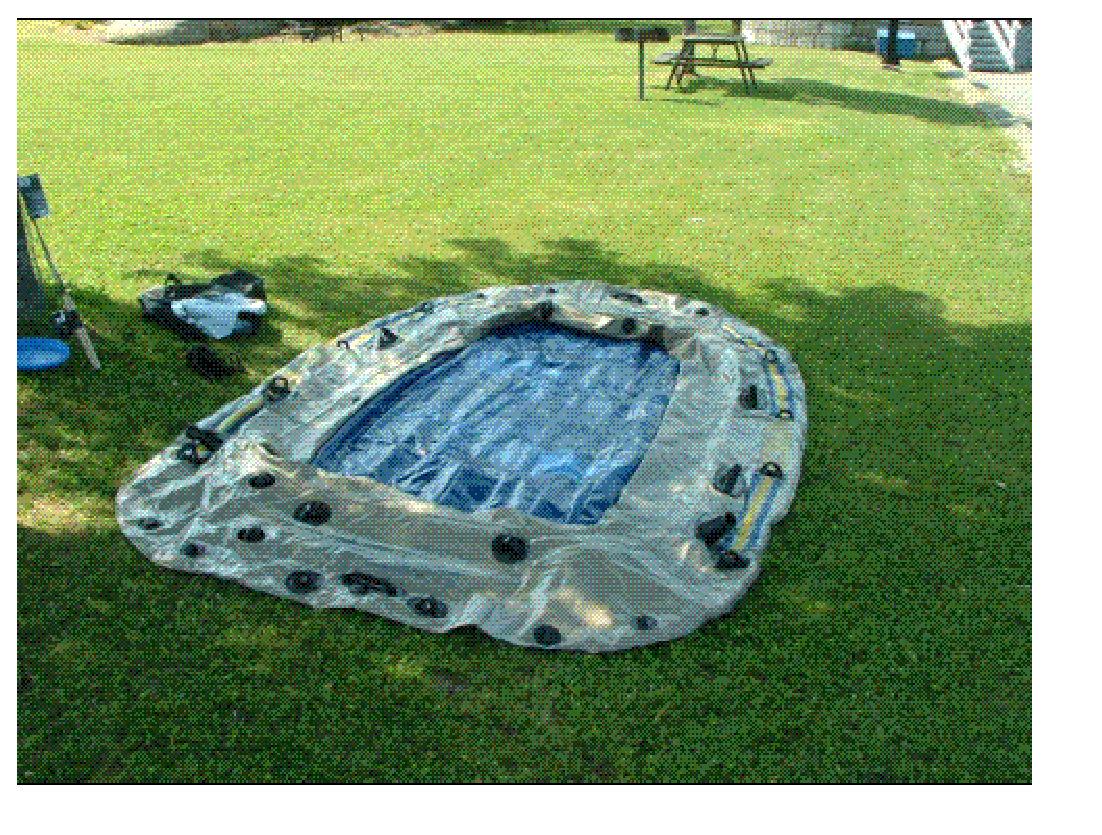
\epsfig{file=fig1.eps,width=3.5in}
Which one of the following is missing in it?
 
 
\noindent{\textbf{\large{
A.}}}
A truck
 
 
\noindent{\textbf{\large{
B.}}}
A frisbee
 
 
\noindent{\textbf{\large{
C.}}}
Lawn
 
 
\noindent{\textbf{\large{
D.}}}
An air-boat
 
 
\noindent{\textbf{\large{
E.}}}
A table
 
 
\noindent{\textbf{\large{
F.}}}
  Not any of aboves.
 
 
\noindent\vspace{0.05in}{\textbf{\Large{Auto-answer:}}}
 
 
\noindent{\textbf{\large{
A.}}}
A truck
 
 
\noindent\vspace{0.05in}{\textbf{\Large{End of auto-answer.}}}
 
 
 
\vspace{0.3in}
   
   
\noindent{\textbf{\Large{Total numbers: }}}
   
   
\noindent\begin{tabular}{|l|l|l|l|l|l|l|}
 \hline
Inputs & Calculates & Choices & Layers & Matches & Answer & Solution \\ \hline
           0  & 
           0  & 
           6
  simple  
  & 
           6  & 
           0  & 
  yes & 
  no 
  \\ \hline
 \end{tabular}
   
   
   
   
\noindent\vspace{0.1in}{\textbf{\Large{Calculated values:}}}
   
   
   
   
\noindent\vspace{0.1in}\hspace{-0.08in} {\textbf{\Large{All inputs: }}}
   
   
  
\vspace{0.2in}
  
{\textbf{\Large{Question
33.1.4 
 (           6 ,          13 ,          28 )
}}}
  
  
What is the operation between $a= % 
7$ and $b= % 
8$:
$a$  % 
$\times$ $b=?$ Please also calculate it.
 
 
\noindent\vspace{0.05in}{\textbf{\Large{Answer:}}}
 
 

7;
 
8;
 
The operation is  % 
MULTIPLICATION and the result is
$ % 
56.000$.
 
 
 
\noindent\vspace{0.05in}{\textbf{\Large{End of Answer.}}}
 
 

 
\vspace{0.3in}
   
   
\noindent{\textbf{\Large{Total numbers: }}}
   
   
\noindent\begin{tabular}{|l|l|l|l|l|l|l|}
 \hline
Inputs & Calculates & Choices & Layers & Matches & Answer & Solution \\ \hline
           3  & 
           2  & 
           0
  & 
           0  & 
           0  & 
  yes & 
  no 
  \\ \hline
 \end{tabular}
   
   
   
   
\noindent\vspace{0.1in}{\textbf{\Large{Calculated values:}}}
   
   
  
  
\noindent\begin{tabular}{|l|l|l|l|}
\hline
 Sequential & Type & Accuracy & Calculated \\ 
\hline
 
 
  Calculated $            1 $ & string & $            1  $ ( $           1  $ strings): 
 & MULTIPLICATION
 \\  \hline  
 
 
  Calculated $            2 $ & real & $            5  $ & 
 $ 56.000 $ 
 \\  \hline  
 \end{tabular}
   
   
   
   
\noindent\vspace{0.1in}\hspace{-0.08in} {\textbf{\Large{All inputs: }}}
   
   
  
  
\noindent\begin{tabular}{|l|l|l|l|l|}
\hline
 Sequential & Type & Accuracy & Three inputs & Generated \\ 
\hline
 
 
  INPUT $            1 $ & integer &  & $
 1
 , 
 10
 , 
 2
 $ & $ 7 $ 
 \\  \hline  
 
 
  INPUT $            2 $ & integer &  & $
 2
 , 
 10
 , 
 2
 $ & $ 8 $ 
 \\  \hline  
 
 
  INPUT $            3 $ & string & & 
 $+$ & 
  \\
  & & & 
 $-$ & 
  \\
  & & & 
 $\times$ & 
  $ <-- $ 
  \\
  & & & 
 $\div$ & 
 \\  \hline  
 \end{tabular}
   
   
  
\vspace{0.2in}
  
{\textbf{\Large{Question
33.1.5 
 (           6 ,          11 ,          26 )
}}}
  
  
In a hotel, the possiblity of  % 
non-smoking customer is
$a =  % 
0.580$, and the possiblity of  % 
 under 30 years old customer is $ b =  % 
4.00 \times 10^{-2}$.
Please calculate the possiblity of  % 
smoking and  % 
equal or above 30 years old customer.
 
 
 
\noindent\vspace{0.1in}{\textbf{\Large{Solution: }}}
 
 

Since the possiblity of  % 
 non-smoking customer is $ a =  % 
0.580 $,
and the possiblity of  % 
 under 30 years old customer is $ b =  % 
4.00 \times 10^{-2} $,
the possiblity of  % 
smoking customer is $ c = 1.0 - a = 1.0 -
0.580
=  % 
0.420 $ and the possiblity of  % 
equal or above 30 years old
customer is $ d = 1.0 - b = 1.0 -  % 
4.00 \times 10^{-2} =  % 
0.9600  $.
So the possibility of  % 
smoking and  % 
equal or above 30 years old
customer is $ c \times d =  % 
0.403 $.
 
 
 
\noindent\vspace{0.1in}{\textbf{\Large{End of Solution.}}}
 
 

 
 
 
\noindent\vspace{0.05in}{\textbf{\Large{Answer:}}}
 
 

The possibility of  % 
smoking and  % 
equal or above 30 years old
customer is $ (1-a)(1-b) =  % 
0.403 $.
 
 
\noindent\vspace{0.05in}{\textbf{\Large{End of Answer.}}}
 
 

 
\vspace{0.3in}
   
   
\noindent{\textbf{\Large{Total numbers: }}}
   
   
\noindent\begin{tabular}{|l|l|l|l|l|l|l|}
 \hline
Inputs & Calculates & Choices & Layers & Matches & Answer & Solution \\ \hline
           4  & 
           3  & 
           0
  & 
           0  & 
           0  & 
  yes & 
  yes 
  \\ \hline
 \end{tabular}
   
   
   
   
\noindent\vspace{0.1in}{\textbf{\Large{Calculated values:}}}
   
   
  
  
\noindent\begin{tabular}{|l|l|l|l|}
\hline
 Sequential & Type & Accuracy & Calculated \\ 
\hline
 
 
  Calculated $            1 $ & real & $            3  $ & 
 $ 0.420 $ 
 \\  \hline  
 
 
  Calculated $            2 $ & real & $            4  $ & 
 $ 0.9600 $ 
 \\  \hline  
 
 
  Calculated $            3 $ & real & $            3  $ & 
 $ 0.403 $ 
 \\  \hline  
 \end{tabular}
   
   
   
   
\noindent\vspace{0.1in}\hspace{-0.08in} {\textbf{\Large{All inputs: }}}
   
   
  
  
\noindent\begin{tabular}{|l|l|l|l|l|}
\hline
 Sequential & Type & Accuracy & Three inputs & Generated \\ 
\hline
 
 
  INPUT $            1 $ & logical & .TRUE. & 
 smoking & 
  \\
  & & .FALSE. & 
  non-smoking & 
  $ <-- $ 
 \\  \hline  
 
 
  INPUT $            2 $ & real & $           -3  $ & $
 1.0 \times 10^{-2}
  $ & \\
  & & &  $
 1.000
  $ & \\
  & & &  $
 1.0 \times 10^{-2}
 $ & $ 0.580 $ 
 \\  \hline  
 
 
  INPUT $            3 $ & logical & .TRUE. & 
 equal or above 30 years old & 
  \\
  & & .FALSE. & 
  under 30 years old & 
  $ <-- $ 
 \\  \hline  
 \end{tabular}
   
   
  
  
\noindent\begin{tabular}{|l|l|l|l|l|}
\hline
 Sequential & Type & Accuracy & Three inputs & Generated \\ 
\hline
 
 
  INPUT $            4 $ & real & $           -4  $ & $
 2.00 \times 10^{-2}
  $ & \\
  & & &  $
 1.0000
  $ & \\
  & & &  $
 2.00 \times 10^{-2}
 $ & $ 4.00 \times 10^{-2} $ 
 \\  \hline  
 \end{tabular}
   
   
  
\vspace{0.2in}
  
{\textbf{\Large{Question
33.1.6 
 (           6 ,          12 ,          27 )
}}}
  
  
In a hotel, the possiblity of  % 
smoking customer is
$a =  % 
0.890$, and the possiblity of  % 
equal-or-above 30 years old customer is $ b =  % 
0.6400$.
Please fill the following form.
 
\noindent
\begin{tabular}{|l|l|}
\hline
Customer & Possibility \\
\hline
smoking  and   % 
equal-or-above 30 years old  & \\
\hline
smoking  and   % 
under 30 years old & \\
\hline
 non-smoking and   % 
equal-or-above 30 years old  & \\
\hline
 non-smoking and  % 
under 30 years old & \\
\hline
\end{tabular}
 
 
 
 
 
\noindent\vspace{0.1in}{\textbf{\Large{Solution: }}}
 
 

Since the possiblity of  % 
smoking customer is $ a =  % 
0.890 $,
and the possiblity of  % 
equal-or-above 30 years old customer is $ b =  % 
0.6400 $,
the possiblity of  % 
non-smoking customer is $ c = 1.0 - a = 1.0 -
0.890
=  % 
0.110 $ and the possiblity of  % 
under 30 years old
customer is $ d = 1.0 - b = 1.0 -  % 
0.6400 =  % 
0.3600  $.
Then
 
\noindent
\begin{tabular}{|l|l|}
\hline
Customer & Possibility \\
\hline
smoking  and  % 
equal-or-above 30 years old  &
  $ % 
0.890 \times  % 
0.6400 =  % 
0.570$ \\
\hline
smoking  and  % 
under 30 years old &
  $ % 
0.890 \times  % 
0.3600 =  % 
0.320$ \\
\hline
 non-smoking and  % 
equal-or-above 30 years old  &
  $ % 
0.110 \times  % 
0.6400 =  % 
7.04 \times 10^{-2}$ \\
\hline
 non-smoking and  % 
under 30 years old &
  $ % 
0.110 \times  % 
0.3600 =  % 
3.96 \times 10^{-2}$ \\
\hline
\end{tabular}
 
\noindent
And the total summation of all possibilities is $  % 
1.000 $.
 
 
 
 
\noindent\vspace{0.1in}{\textbf{\Large{End of Solution.}}}
 
 

 
 
 
\noindent\vspace{0.05in}{\textbf{\Large{Answer:}}}
 
 

 
\noindent
\begin{tabular}{|l|l|}
\hline
Customer & Possibility \\
\hline
smoking  and  % 
equal-or-above 30 years old &
  $ % 
0.570$ \\
\hline
smoking  and  % 
under 30 years old &
  $ % 
0.320$ \\
\hline
 non-smoking and  % 
equal-or-above 30 years old &
  $ % 
7.04 \times 10^{-2}$ \\
\hline
 non-smoking and  % 
under 30 years old &
  $ % 
3.96 \times 10^{-2}$ \\
\hline
\end{tabular}
 
\noindent
 And the total summation of all possibilities is $  % 
1.000 $.
 
 
 
\noindent\vspace{0.05in}{\textbf{\Large{End of Answer.}}}
 
 

 
\vspace{0.3in}
   
   
\noindent{\textbf{\Large{Total numbers: }}}
   
   
\noindent\begin{tabular}{|l|l|l|l|l|l|l|}
 \hline
Inputs & Calculates & Choices & Layers & Matches & Answer & Solution \\ \hline
           4  & 
          11  & 
           0
  & 
           0  & 
           0  & 
  yes & 
  yes 
  \\ \hline
 \end{tabular}
   
   
   
   
\noindent\vspace{0.1in}{\textbf{\Large{Calculated values:}}}
   
   
  
  
\noindent\begin{tabular}{|l|l|l|l|}
\hline
 Sequential & Type & Accuracy & Calculated \\ 
\hline
 
 
  Calculated $            1 $ & real & $            3  $ & 
 $ 0.110 $ 
 \\  \hline  
 
 
  Calculated $            2 $ & real & $            4  $ & 
 $ 0.3600 $ 
 \\  \hline  
 
 
  Calculated $            3 $ & real & $            3  $ & 
 $ 0.890 $ 
 \\  \hline  
 
 
  Calculated $            4 $ & real & $            3  $ & 
 $ 0.110 $ 
 \\  \hline  
 
 
  Calculated $            5 $ & real & $            4  $ & 
 $ 0.6400 $ 
 \\  \hline  
 
 
  Calculated $            6 $ & real & $            4  $ & 
 $ 0.3600 $ 
 \\  \hline  
 
 
  Calculated $            7 $ & real & $            3  $ & 
 $ 0.570 $ 
 \\  \hline  
 
 
  Calculated $            8 $ & real & $            3  $ & 
 $ 0.320 $ 
 \\  \hline  
 
 
  Calculated $            9 $ & real & $            3  $ & 
 $ 7.04 \times 10^{-2} $ 
 \\  \hline  
 
 
  Calculated $           10 $ & real & $            3  $ & 
 $ 3.96 \times 10^{-2} $ 
 \\  \hline  
 \end{tabular}
   
   
  
  
\noindent\begin{tabular}{|l|l|l|l|}
\hline
 Sequential & Type & Accuracy & Calculated \\ 
\hline
 
 
  Calculated $           11 $ & real & $            4  $ & 
 $ 1.000 $ 
 \\  \hline  
 \end{tabular}
   
   
   
   
\noindent\vspace{0.1in}\hspace{-0.08in} {\textbf{\Large{All inputs: }}}
   
   
  
  
\noindent\begin{tabular}{|l|l|l|l|l|}
\hline
 Sequential & Type & Accuracy & Three inputs & Generated \\ 
\hline
 
 
  INPUT $            1 $ & logical & .TRUE. & 
 smoking & 
  $ <-- $ 
  \\
  & & .FALSE. & 
  non-smoking & 
 \\  \hline  
 
 
  INPUT $            2 $ & real & $           -3  $ & $
 1.0 \times 10^{-2}
  $ & \\
  & & &  $
 1.000
  $ & \\
  & & &  $
 1.0 \times 10^{-2}
 $ & $ 0.890 $ 
 \\  \hline  
 
 
  INPUT $            3 $ & logical & .TRUE. & 
 equal-or-above 30 years old & 
  $ <-- $ 
  \\
  & & .FALSE. & 
  under 30 years old & 
 \\  \hline  
 \end{tabular}
   
   
  
  
\noindent\begin{tabular}{|l|l|l|l|l|}
\hline
 Sequential & Type & Accuracy & Three inputs & Generated \\ 
\hline
 
 
  INPUT $            4 $ & real & $           -4  $ & $
 2.00 \times 10^{-2}
  $ & \\
  & & &  $
 1.0000
  $ & \\
  & & &  $
 2.00 \times 10^{-2}
 $ & $ 0.6400 $ 
 \\  \hline  
 \end{tabular}
   
   
   
   
\vspace{0.3in}
{\textbf{\LARGE{You have done all the above? A very good beginning, please go ahead.}}}
More constants the
Mass of electron
$m_e$$ =
9.109390 \times 10^{-31} $
kg
,
Universal gas constant
$R$$ =
8.315 $
J/(mol$\cdot $K)
,
$e$$ =
1.60217733 \times 10^{-19} $
C
, and
$m_p$$ =
1.6726231 \times 10^{-27} $
kg
%
may be very helpful.
\vspace{0.3in}
   
   
  
\vspace{0.2in}
  
{\textbf{\Large{QUESTION
33.2 
 (           4 ,           4 ,           4 )
}}}
  
  
Considering case-insensitivity, please match the following same strings.
  
  
\begin{tabular}{|l|l|l|}
 \hline
 Column Left & Column Right  & Your choinces \\ 
 \hline
{\textbf{\large{
A.}}}
asdf(:)
  & 
c
 & 
 \\ 
 \hline
{\textbf{\large{
B.}}}
C
  & 
ER
 & 
 \\ 
 \hline
{\textbf{\large{
C.}}}
Er
  & 
b
 & 
 \\ 
 \hline
{\textbf{\large{
D.}}}
B
  & 
ASDF(:)
 & 
 \\ 
 \hline
{\textbf{\large{
E.}}}
A
  & 
a
 & 
 \\ 
 \hline
 \end{tabular}
  
  
 
 
\noindent\vspace{0.05in}{\textbf{\Large{Auto-answer:}}}
  
  
\begin{tabular}{|l|l|l|}
 \hline
 Column Left & Column Right  & Answers       \\ 
 \hline
{\textbf{\large{
A.}}}
asdf(:)
  & 
c
 & 
{\textbf{\large{
B.}}}
 \\ 
 \hline
{\textbf{\large{
B.}}}
C
  & 
ER
 & 
{\textbf{\large{
C.}}}
 \\ 
 \hline
{\textbf{\large{
C.}}}
Er
  & 
b
 & 
{\textbf{\large{
D.}}}
 \\ 
 \hline
{\textbf{\large{
D.}}}
B
  & 
ASDF(:)
 & 
{\textbf{\large{
A.}}}
 \\ 
 \hline
{\textbf{\large{
E.}}}
A
  & 
a
 & 
{\textbf{\large{
E.}}}
 \\ 
 \hline
 \end{tabular}
  
  
 
 
\noindent\vspace{0.05in}{\textbf{\Large{End of auto-answer.}}}
 
 
 
   
   
\noindent{\textbf{\Large{Total numbers: }}}
   
   
\noindent\begin{tabular}{|l|l|l|l|l|l|l|}
 \hline
Inputs & Calculates & Choices & Layers & Matches & Answer & Solution \\ \hline
           2  & 
           1  & 
           0
  & 
          16  & 
           5  & 
  yes & 
  no 
  \\ \hline
 \end{tabular}
   
   
   
   
\noindent\vspace{0.1in}{\textbf{\Large{Calculated values:}}}
   
   
  
  
\noindent\begin{tabular}{|l|l|l|l|}
\hline
 Sequential & Type & Accuracy & Calculated \\ 
\hline
 
 
  Calculated $            1 $ & integer &  & 
  $ 1 $ 
 \\  \hline  
 \end{tabular}
   
   
   
   
\noindent\vspace{0.1in}\hspace{-0.08in} {\textbf{\Large{All inputs: }}}
   
   
  
  
\noindent\begin{tabular}{|l|l|l|l|l|}
\hline
 Sequential & Type & Accuracy & Three inputs & Generated \\ 
\hline
 
 
  INPUT $            1 $ & integer &  & $
 2
 , 
 8
 , 
 2
 $ & $ 2 $ 
 \\  \hline  
 
 
  INPUT $            2 $ & integer &  & $
 2
 , 
 3
 , 
 2
 $ & $ 2 $ 
 \\  \hline  
 \end{tabular}
   
   
  
\vspace{0.2in}
  
{\textbf{\Large{QUESTION
33.3 
 (           3 ,           3 ,           3 )
}}}
  
  
Please choose the correct one from the following statements:
 
 
\noindent{\textbf{\large{
A.}}}
Canada has  %
36 provinces and  %
35 territories.
 
 
\noindent{\textbf{\large{
B.}}}
Canada has  %
10 provinces and  %
3 territories.
 
 
\noindent{\textbf{\large{
C.}}}
Canada has  %
33 provinces and  %
38 territories.
 
 
\noindent{\textbf{\large{
D.}}}
Canada has  %
37 provinces and  %
37 territories.
 
 
\noindent{\textbf{\large{
E.}}}
Canada has  %
34 provinces and  %
39 territories.
 
 
\noindent{\textbf{\large{
F.}}}
 None of above.
 
 
\noindent\vspace{0.05in}{\textbf{\Large{Auto-answer:}}}
 
 
\noindent{\textbf{\large{
B.}}}
Canada has  %
10 provinces and  %
3 territories.
 
 
\noindent\vspace{0.05in}{\textbf{\Large{End of auto-answer.}}}
 
 
   
   
\noindent{\textbf{\Large{Total numbers: }}}
   
   
\noindent\begin{tabular}{|l|l|l|l|l|l|l|}
 \hline
Inputs & Calculates & Choices & Layers & Matches & Answer & Solution \\ \hline
           0  & 
          20  & 
           6
  simple  
  & 
           6  & 
           0  & 
  yes & 
  no 
  \\ \hline
 \end{tabular}
   
   
   
   
\noindent\vspace{0.1in}{\textbf{\Large{Calculated values:}}}
   
   
  
  
\noindent\begin{tabular}{|l|l|l|l|}
\hline
 Sequential & Type & Accuracy & Calculated \\ 
\hline
 
 
  Calculated $            1 $ & integer &  & 
  $ 10 $ 
 \\  \hline  
 
 
  Calculated $            2 $ & integer &  & 
  $ 3 $ 
 \\  \hline  
 
 
  Calculated $            3 $ & integer &  & 
  $ 23 $ 
 \\  \hline  
 
 
  Calculated $            4 $ & integer &  & 
  $ 24 $ 
 \\  \hline  
 
 
  Calculated $            5 $ & integer &  & 
  $ 25 $ 
 \\  \hline  
 
 
  Calculated $            6 $ & integer &  & 
  $ 26 $ 
 \\  \hline  
 
 
  Calculated $            7 $ & integer &  & 
  $ 27 $ 
 \\  \hline  
 
 
  Calculated $            8 $ & integer &  & 
  $ 28 $ 
 \\  \hline  
 
 
  Calculated $            9 $ & integer &  & 
  $ 29 $ 
 \\  \hline  
 
 
  Calculated $           10 $ & integer &  & 
  $ 30 $ 
 \\  \hline  
 \end{tabular}
   
   
  
  
\noindent\begin{tabular}{|l|l|l|l|}
\hline
 Sequential & Type & Accuracy & Calculated \\ 
\hline
 
 
  Calculated $           11 $ & integer &  & 
  $ 31 $ 
 \\  \hline  
 
 
  Calculated $           12 $ & integer &  & 
  $ 32 $ 
 \\  \hline  
 
 
  Calculated $           13 $ & integer &  & 
  $ 33 $ 
 \\  \hline  
 
 
  Calculated $           14 $ & integer &  & 
  $ 34 $ 
 \\  \hline  
 
 
  Calculated $           15 $ & integer &  & 
  $ 35 $ 
 \\  \hline  
 
 
  Calculated $           16 $ & integer &  & 
  $ 36 $ 
 \\  \hline  
 
 
  Calculated $           17 $ & integer &  & 
  $ 37 $ 
 \\  \hline  
 
 
  Calculated $           18 $ & integer &  & 
  $ 38 $ 
 \\  \hline  
 
 
  Calculated $           19 $ & integer &  & 
  $ 39 $ 
 \\  \hline  
 
 
  Calculated $           20 $ & integer &  & 
  $ 40 $ 
 \\  \hline  
 \end{tabular}
   
   
   
   
\noindent\vspace{0.1in}\hspace{-0.08in} {\textbf{\Large{All inputs: }}}
   
   
  
\vspace{0.2in}
  
{\textbf{\Large{QUESTION
33.4 
 (           2 ,           2 ,           2 )
}}}
  
  
 
An object is subjected to an external net force $\mathbf{f}=(
60.000 ,
4.0000,
-8000.0  )N$. Its mass is known as
$m= % 
54.0000  kg$. Please choose the correct accelaration
from the following choices.
 
 
 
\noindent{\textbf{\large{
A.}}}
The accelaration is
$(
2.8796ms^{-2},
960.00km/h^2,
-689.97ms^{-2}
).
$
 
 
\noindent{\textbf{\large{
B.}}}
The accelaration is
$(
2.8796ms^{-2},
960.00km/h^2,
-148.15ms^{-2}
).
$
 
 
\noindent{\textbf{\large{
C.}}}
The accelaration is
$(
1.1111ms^{-2},
960.00km/h^2,
-689.97ms^{-2}
).
$
 
 
\noindent{\textbf{\large{
D.}}}
The accelaration is
$(
1.1111ms^{-2},
-4116.1km/h^2,
-148.15ms^{-2}
).
$
 
 
\noindent{\textbf{\large{
E.}}}
The accelaration is
$(
1.1111ms^{-2},
960.00km/h^2,
-148.15ms^{-2}
).
$
 
 
\noindent{\textbf{\large{
F.}}}
The accelaration is
$(
2.8796ms^{-2},
-4116.1km/h^2,
-148.15ms^{-2}
).
$
 
 
\noindent{\textbf{\large{
G.}}}
 None of these.
 
 
\noindent\vspace{0.05in}{\textbf{\Large{Auto-answer:}}}
 
 
\noindent{\textbf{\large{
E.}}}
The accelaration is
$(
1.1111ms^{-2},
960.00km/h^2,
-148.15ms^{-2}
).
$
 
 
\noindent\vspace{0.05in}{\textbf{\Large{End of auto-answer.}}}
 
 
 
 
 
 
\noindent\vspace{0.1in}{\textbf{\Large{Solution: }}}
 
 

We will use the Newton's Second Law:
 
\[
\mathbf{f}=m\mathbf{a}.
\]
 
Since $\mathbf{f}=( % 
60.000,  % 
4.0000,  % 
-8000.0 )N$
and $m= % 
54.0000kg$, bring them into the above equation, then we get
 
\begin{eqnarray*}
\mathbf{a}&=&\frac{\mathbf{f}}m  \\
&=&\frac{(
60.000 ,
4.0000 ,
-8000.0 )N
}{ % 
54.0000 kg}  \\
&=&(
1.1111 ,
7.4074 \times 10^{-2},
-148.15
)ms^{-2} \\
&=&(
14400. ,
960.00 ,
-1.9200 \times 10^{6}
)km/h^2.
\end{eqnarray*}
 
 
 
\noindent\vspace{0.1in}{\textbf{\Large{End of Solution.}}}
 
 

 
\vspace{0.3in}
   
   
\noindent{\textbf{\Large{Total numbers: }}}
   
   
\noindent\begin{tabular}{|l|l|l|l|l|l|l|}
 \hline
Inputs & Calculates & Choices & Layers & Matches & Answer & Solution \\ \hline
           4  & 
           6  & 
           7
  & 
           3  & 
           0  & 
  yes & 
  yes 
  \\ \hline
 \end{tabular}
   
   
   
   
\noindent\vspace{0.1in}{\textbf{\Large{Calculated values:}}}
   
   
  
  
\noindent\begin{tabular}{|l|l|l|l|}
\hline
 Sequential & Type & Accuracy & Calculated \\ 
\hline
 
 
  Calculated $            1 $ & real & $            5  $ & 
 $ 1.1111 $ 
 \\  \hline  
 
 
  Calculated $            2 $ & real & $            5  $ & 
 $ 7.4074 \times 10^{-2} $ 
 \\  \hline  
 
 
  Calculated $            3 $ & real & $            5  $ & 
 $ -148.15 $ 
 \\  \hline  
 
 
  Calculated $            4 $ & real & $            5  $ & 
 $ 14400. $ 
 \\  \hline  
 
 
  Calculated $            5 $ & real & $            5  $ & 
 $ 960.00 $ 
 \\  \hline  
 
 
  Calculated $            6 $ & real & $            5  $ & 
 $ -1.9200 \times 10^{6} $ 
 \\  \hline  
 \end{tabular}
   
   
   
   
\noindent\vspace{0.1in}\hspace{-0.08in} {\textbf{\Large{All inputs: }}}
   
   
  
  
\noindent\begin{tabular}{|l|l|l|l|l|}
\hline
 Sequential & Type & Accuracy & Three inputs & Generated \\ 
\hline
 
 
  INPUT $            1 $ & real & $           -3  $ & $
 20.000
  $ & \\
  & & &  $
 101.000
  $ & \\
  & & &  $
 10.000
 $ & $ 60.000 $ 
 \\  \hline  
 
 
  INPUT $            2 $ & real & $           -4  $ & $
 2.0000
  $ & \\
  & & &  $
 10.1000
  $ & \\
  & & &  $
 1.0000
 $ & $ 4.0000 $ 
 \\  \hline  
 
 
  INPUT $            3 $ & real & $           -1  $ & $
 -2000.0
  $ & \\
  & & &  $
 -10001.0
  $ & \\
  & & &  $
 -1000.0
 $ & $ -8000.0 $ 
 \\  \hline  
 \end{tabular}
   
   
  
  
\noindent\begin{tabular}{|l|l|l|l|l|}
\hline
 Sequential & Type & Accuracy & Three inputs & Generated \\ 
\hline
 
 
  INPUT $            4 $ & real & $           -4  $ & $
 50.0000
  $ & \\
  & & &  $
 60.1000
  $ & \\
  & & &  $
 2.0000
 $ & $ 54.0000 $ 
 \\  \hline  
 \end{tabular}
   
   
  
\vspace{0.2in}
  
{\textbf{\Large{QUESTION
33.5 
 (           1 ,           1 ,           1 )
}}}
  
  


\noindent\vspace{0.05in}{\textbf{\Large{Abstract:}}}
This is a simple Newton's Second Law calculation multi-choice problem.  
\noindent\vspace{0.05in}{\textbf{\Large{end of abstract.}}}


 
 
An object is subjected to an external net force $\mathbf{f}=
(50.0 , 4.0 , -2000.0) N$.
Its mass is known as $m= % 
60.0000 kg$. Please choose the
correct accelaration from the following choices.
 
 
 
\noindent{\textbf{\large{
A.}}}
The accelaration is $  %
(
0.833,
6.7 \times 10^{-2},
159.20)
ms^{-2} $.
 
 
\noindent{\textbf{\large{
B.}}}
The accelaration is $  %
(
0.833,
0.28,
-33.333)
ms^{-2} $.
 
 
\noindent{\textbf{\large{
C.}}}
The accelaration is $  %
(
0.833,
6.7 \times 10^{-2},
-33.333)
ms^{-2} $.
 
 
\noindent{\textbf{\large{
D.}}}
The accelaration is $  %
(
2.49,
0.28,
-33.333)
ms^{-2} $.
 
 
\noindent{\textbf{\large{
E.}}}
The accelaration is $  %
(
2.49,
6.7 \times 10^{-2},
-33.333)
ms^{-2} $.
 
 
\noindent{\textbf{\large{
F.}}}
The accelaration is $  %
(
2.49,
0.28,
159.20)
ms^{-2} $.
 
 
\noindent{\textbf{\large{
G.}}}
The accelaration is $  %
(
2.49,
6.7 \times 10^{-2},
159.20)
ms^{-2} $.
 
 
\noindent{\textbf{\large{
H.}}}
The accelaration is $  %
(
0.833,
0.28,
159.20)
ms^{-2} $.
 
 
\noindent\vspace{0.05in}{\textbf{\Large{Auto-answer:}}}
 
 
\noindent{\textbf{\large{
C.}}}
The accelaration is $  %
(
0.833,
6.7 \times 10^{-2},
-33.333)
ms^{-2} $.
 
 
\noindent\vspace{0.05in}{\textbf{\Large{End of auto-answer.}}}
 
 
 
 
 
\noindent\vspace{0.05in}{\textbf{\Large{Answer:}}}
 
 

The correct answer from the choices is


\noindent{\textbf{\large{
C.}}}
The accelaration is $  %
(
0.833,
6.7 \times 10^{-2},
-33.333)
ms^{-2} $.
 
 
 
\noindent\vspace{0.05in}{\textbf{\Large{End of Answer.}}}
 
 

 
 
 
\noindent\vspace{0.1in}{\textbf{\Large{Solution: }}}
 
 

We will use the Newton's Second Law:
 
\[
\mathbf{f}=m\mathbf{a}.
\]
 
Since $\mathbf{f}= % 
(50.0 , 4.0 , -2000.0) N$
and $m= % 
60.0000kg$, bring them into the above equation, then we get
 
\begin{eqnarray*}
\mathbf{a}&=&\frac{\mathbf{f}}m  \\
&=&\frac{ % 
(50.0 , 4.0 , -2000.0) N}{ % 
60.0000kg}  \\
&=& % 
(0.833 , 6.7 \times 10^{-2} , -33.333) ms^{-2}
\end{eqnarray*}
 
 
 
\noindent\vspace{0.1in}{\textbf{\Large{End of Solution.}}}
 
 

 
\vspace{0.3in}
   
   
\noindent{\textbf{\Large{Total numbers: }}}
   
   
\noindent\begin{tabular}{|l|l|l|l|l|l|l|}
 \hline
Inputs & Calculates & Choices & Layers & Matches & Answer & Solution \\ \hline
           2  & 
           1  & 
           8
  & 
           3  & 
           0  & 
  yes & 
  yes 
  \\ \hline
 \end{tabular}
   
   
   
   
\noindent\vspace{0.1in}{\textbf{\Large{Calculated values:}}}
   
   
  
  
\noindent\begin{tabular}{|l|l|l|l|}
\hline
 Sequential & Type & Accuracy & Calculated \\ 
\hline
 
 
  Calculated $            1 $ & vector &  
  $            3  $ 
 &  $ 0.833 $ 
 \\    
  & & 
  $            2  $ 
 &  $ 6.7 \times 10^{-2} $ 
 \\    
  & & 
  $            5  $ 
 &  $ -33.333 $ 
 \\  \hline  
 \end{tabular}
   
   
   
   
\noindent\vspace{0.1in}\hspace{-0.08in} {\textbf{\Large{All inputs: }}}
   
   
  
  
\noindent\begin{tabular}{|l|l|l|l|l|}
\hline
 Sequential & Type & Accuracy & Three inputs & Generated \\ 
\hline
 
 
  INPUT $            1 $ & vector & $           -1  $ & $
20.0
  $ & \\
  & & & $
101.0
  $ & \\
  & & & $
10.0
$ & $ 50.0 $ 
  \\
  & & $           -1  $ & $
2.0
  $ & \\
  & & & $
10.1
  $ & \\
  & & & $
1.0
$ & $ 4.0 $ 
  \\
  & & $           -1  $ & $
-2000.0
  $ & \\
  & & & $
-10001.0
  $ & \\
  & & & $
-1000.0
$ & $ -2000.0 $ 
 \\  \hline  
 
 
  INPUT $            2 $ & real & $           -4  $ & $
 50.0000
  $ & \\
  & & &  $
 60.1000
  $ & \\
  & & &  $
 2.0000
 $ & $ 60.0000 $ 
 \\  \hline  
 \end{tabular}
   
   
  
\vspace{0.2in}
  
{\textbf{\Large{QUESTION
33.6 
 (           5 ,           5 ,           5 )
}}}
  
  
If any one of the following statements is correct, please fill the box ahead of it with $T$ .
If wrong, fill with $F$.
 
\noindent\begin{tabular}{|l|l|}\hline Your&\hspace{.2in} \\ answer&\hspace{.2in} \\ \hline \end{tabular}
1. $ % 
9$ is an  % 
even number.
 
\noindent\begin{tabular}{|l|l|}\hline Your&\hspace{.2in} \\ answer&\hspace{.2in} \\ \hline \end{tabular}
2.  % 
Toronto is in  % 
Ontario province.
 
\noindent\begin{tabular}{|l|l|}\hline Your&\hspace{.2in} \\ answer&\hspace{.2in} \\ \hline \end{tabular}
3.  % 
$\mathbf{F}=m\mathbf{a}$ is a mathmatical form of
the Newton's Second Law.
 
 
 
\noindent\vspace{0.05in}{\textbf{\Large{Answer:}}}
 
 

 
\noindent\begin{tabular}{|l|l|}\hline The correct & \\
          answer &  % 
$F$ \\ \hline \end{tabular}
1. $ % 
9$ is an  % 
even number.
 
\noindent\begin{tabular}{|l|l|}\hline The correct & \\
          answer &  % 
$T$ \\ \hline \end{tabular}
2.  % 
Toronto is in  % 
Ontario province.
 
\noindent\begin{tabular}{|l|l|}\hline The correct & \\
          answer &  % 
$T$ \\ \hline \end{tabular}
3.  % 
$\mathbf{F}=m\mathbf{a}$ is a mathmatical form of  % 
the Newton's Second Law.
 
 
 
\noindent\vspace{0.05in}{\textbf{\Large{End of Answer.}}}
 
 

 
\vspace{0.3in}
   
   
\noindent{\textbf{\Large{Total numbers: }}}
   
   
\noindent\begin{tabular}{|l|l|l|l|l|l|l|}
 \hline
Inputs & Calculates & Choices & Layers & Matches & Answer & Solution \\ \hline
           6  & 
           3  & 
           0
  & 
           0  & 
           0  & 
  yes & 
  no 
  \\ \hline
 \end{tabular}
   
   
   
   
\noindent\vspace{0.1in}{\textbf{\Large{Calculated values:}}}
   
   
  
  
\noindent\begin{tabular}{|l|l|l|l|}
\hline
 Sequential & Type & Accuracy & Calculated \\ 
\hline
 
 
  Calculated $            1 $ & string & $            1  $ ( $           1  $ strings): 
 & $F$
 \\  \hline  
 
 
  Calculated $            2 $ & string & $            1  $ ( $           1  $ strings): 
 & $T$
 \\  \hline  
 
 
  Calculated $            3 $ & string & $            1  $ ( $           1  $ strings): 
 & $T$
 \\  \hline  
 \end{tabular}
   
   
   
   
\noindent\vspace{0.1in}\hspace{-0.08in} {\textbf{\Large{All inputs: }}}
   
   
  
  
\noindent\begin{tabular}{|l|l|l|l|l|}
\hline
 Sequential & Type & Accuracy & Three inputs & Generated \\ 
\hline
 
 
  INPUT $            1 $ & integer &  & $
 1
 , 
 100
 , 
 1
 $ & $ 9 $ 
 \\  \hline  
 
 
  INPUT $            2 $ & string & & 
 even & 
  $ <-- $ 
  \\
  & & & 
 odd & 
 \\  \hline  
 
 
  INPUT $            3 $ & string & & 
 Toronto & 
  $ <-- $ 
  \\
  & & & 
 Kingston & 
  \\
  & & & 
 Montreal & 
  \\
  & & & 
 Hull & 
 \\  \hline  
 \end{tabular}
   
   
  
  
\noindent\begin{tabular}{|l|l|l|l|l|}
\hline
 Sequential & Type & Accuracy & Three inputs & Generated \\ 
\hline
 
 
  INPUT $            4 $ & string & & 
 Ontario & 
  $ <-- $ 
  \\
  & & & 
 Quebec & 
 \\  \hline  
 
 
  INPUT $            5 $ & string & & 
 $\mathbf{F}=m\mathbf{a}$ & 
  $ <-- $ 
  \\
  & & & 
 $\left| \mathbf{F}\right| =Gm_1m_2r^{-2}$ & 
 \\  \hline  
 
 
  INPUT $            6 $ & string & & 
 the Newton's Second Law & 
  $ <-- $ 
  \\
  & & & 
 Newton's Law of Universal Gravitation & 
 \\  \hline  
 \end{tabular}
   
   
   
   
\vspace{0.3in}
{\textbf{\LARGE{You have done all the above? Excellent! Not much left, please continue.}}}
\vspace{0.3in}
   
   
  
\vspace{0.2in}
  
{\textbf{\Large{QUESTION
33.7 
 (           7 ,          14 ,          50 )
}}}
  
  
 
An object is subjected to an external net force $\mathbf{f}=
(70.0 , 9.0 , -7000.0) N$.
Its mass is known as $m= % 
58.0 kg$.
Please choose the correct accelaration from the following choices.
 
 
\noindent{\textbf{\large{
A.}}}
  The accelaration is $  %
(
1.21,
0.16,
-120.69)
ms^{-2} $.
 
 
\noindent{\textbf{\large{
B.}}}
  The accelaration is $  %
(
4.23,
0.58,
-285.99)
ms^{-2} $.
 
 
\noindent{\textbf{\large{
C.}}}
  The accelaration is $  %
(
1.21,
0.16,
-285.99)
ms^{-2} $.
 
 
\noindent{\textbf{\large{
D.}}}
  The accelaration is $  %
(
4.23,
0.58,
-120.69)
ms^{-2} $.
 
 
\noindent\vspace{0.05in}{\textbf{\Large{Auto-answer:}}}
 
 
\noindent{\textbf{\large{
A.}}}
  The accelaration is $  %
(
1.21,
0.16,
-120.69)
ms^{-2} $.
 
 
\noindent\vspace{0.05in}{\textbf{\Large{End of auto-answer.}}}
 
 
 
 
 
\noindent\vspace{0.1in}{\textbf{\Large{Solution: }}}
 
 

We will use the Newton's Second Law:
 
\[
\mathbf{f}=m\mathbf{a}.
\]
 
Since $\mathbf{f}= % 
(70.0 , 9.0 , -7000.0) N$
and $m= % 
58.0kg$, bring them into the above equation, then we get
 
\begin{eqnarray*}
\mathbf{a}&=&\frac{\mathbf{f}}m  \\
&=&\frac{ % 
(70.0 , 9.0 , -7000.0) N}{ % 
58.0kg}  \\
&=& % 
(1.21 , 0.16 , -120.69) ms^{-2}
\end{eqnarray*}
 
 
 
\noindent\vspace{0.1in}{\textbf{\Large{End of Solution.}}}
 
 

 
 
\vspace{0.3in}
   
   
\noindent{\textbf{\Large{Total numbers: }}}
   
   
\noindent\begin{tabular}{|l|l|l|l|l|l|l|}
 \hline
Inputs & Calculates & Choices & Layers & Matches & Answer & Solution \\ \hline
           2  & 
           1  & 
           4
  & 
           3  & 
           0  & 
  yes & 
  yes 
  \\ \hline
 \end{tabular}
   
   
   
   
\noindent\vspace{0.1in}{\textbf{\Large{Calculated values:}}}
   
   
  
  
\noindent\begin{tabular}{|l|l|l|l|}
\hline
 Sequential & Type & Accuracy & Calculated \\ 
\hline
 
 
  Calculated $            1 $ & vector &  
  $            3  $ 
 &  $ 1.21 $ 
 \\    
  & & 
  $            2  $ 
 &  $ 0.16 $ 
 \\    
  & & 
  $            5  $ 
 &  $ -120.69 $ 
 \\  \hline  
 \end{tabular}
   
   
   
   
\noindent\vspace{0.1in}\hspace{-0.08in} {\textbf{\Large{All inputs: }}}
   
   
  
  
\noindent\begin{tabular}{|l|l|l|l|l|}
\hline
 Sequential & Type & Accuracy & Three inputs & Generated \\ 
\hline
 
 
  INPUT $            1 $ & vector & $           -1  $ & $
20.0
  $ & \\
  & & & $
101.0
  $ & \\
  & & & $
10.0
$ & $ 70.0 $ 
  \\
  & & $           -1  $ & $
2.0
  $ & \\
  & & & $
10.1
  $ & \\
  & & & $
1.0
$ & $ 9.0 $ 
  \\
  & & $           -1  $ & $
-2000.0
  $ & \\
  & & & $
-10001.0
  $ & \\
  & & & $
-1000.0
$ & $ -7000.0 $ 
 \\  \hline  
 
 
  INPUT $            2 $ & real & $           -1  $ & $
 50.0
  $ & \\
  & & &  $
 60.1
  $ & \\
  & & &  $
 2.0
 $ & $ 58.0 $ 
 \\  \hline  
 \end{tabular}
   
   
  
\vspace{0.2in}
  
{\textbf{\Large{QUESTION
33.8 
 (           8 ,          15 ,          60 )
}}}
  
  
 
$ \left( \begin{array}{ccccccccc}
           5  & 
           6  & 
           6  & 
           4  \\ 
           4  & 
           5  & 
           6  & 
           6  \\ 
           7  & 
           5  & 
           4  & 
           5
\end{array}\right) \times
\left( \begin{array}{c}
           2  \\ 
           2  \\ 
           2  \\ 
           2
\end{array}\right) $ =?
 
 
$  % 
 \left( \begin{array}
 {
 c
 c
 }
 \Theta & 
 \Lambda \\ 
 \gamma & 
 \delta \\ 
 \Lambda & 
 \varepsilon \\ 
 \alpha & 
                    \Xi
 \end{array} \right)
 \left( \begin{array}
 {
 c
 }
 \beta \\ 
 \beta
 \end{array} \right)
$ =?
 
 
 
\noindent\vspace{0.05in}{\textbf{\Large{Answer:}}}
 
 

 
$\left( \begin{array}{ccccccccccccccc}
           5  & 
           6  & 
           6  & 
           4  \\ 
           4  & 
           5  & 
           6  & 
           6  \\ 
           7  & 
           5  & 
           4  & 
           5
\end{array}\right) \times
\left( \begin{array}{c}
           2  \\ 
           2  \\ 
           2  \\ 
           2
\end{array}\right)  =
\left( \begin{array}{c}
          42  \\ 
          42  \\ 
          42
\end{array}\right)  $
 
$  % 
 \left( \begin{array}
 {
 c
 c
 }
 \Theta & 
 \Lambda \\ 
 \gamma & 
 \delta \\ 
 \Lambda & 
 \varepsilon \\ 
 \alpha & 
                    \Xi
 \end{array} \right)
 \left( \begin{array}
 {
 c
 }
 \beta \\ 
 \beta
 \end{array} \right)
=
 \left( \begin{array}
 {
 c
 }
  \Theta \times  \beta +  \Lambda \times  \beta \\ 
  \gamma \times  \beta +  \delta \times  \beta \\ 
  \Lambda \times  \beta +  \varepsilon \times  \beta \\ 
  \alpha \times  \beta +                     \Xi \times  \beta
 \end{array} \right)
$
 
 
 
\noindent\vspace{0.05in}{\textbf{\Large{End of Answer.}}}
 
 

 
 
 
\noindent\vspace{0.1in}{\textbf{\Large{Solution: }}}
 
 

 
 
\noindent\vspace{0.1in}{\textbf{\Large{End of Solution.}}}
 
 

 
\vspace{0.3in}
   
   
\noindent{\textbf{\Large{Total numbers: }}}
   
   
\noindent\begin{tabular}{|l|l|l|l|l|l|l|}
 \hline
Inputs & Calculates & Choices & Layers & Matches & Answer & Solution \\ \hline
           4  & 
           2  & 
           0
  & 
           0  & 
           0  & 
  yes & 
  yes 
  \\ \hline
 \end{tabular}
   
   
   
   
\noindent\vspace{0.1in}{\textbf{\Large{Calculated values:}}}
   
   
  
  
\noindent\begin{tabular}{|l|l|l|l|}
\hline
 Sequential & Type & Accuracy & Calculated \\ 
\hline
 
 
  Calculated $            1 $ & i-matrix &  & 
 (size:            3  by            1 )
 \\  \hline  
 \end{tabular}
   
   
$\begin{array}{
 c
 }
          42  \\ 
          42  \\ 
          42
 \end{array}  $ 
  
  
\noindent\begin{tabular}{|l|l|l|l|}
\hline
 Sequential & Type & Accuracy & Calculated \\ 
\hline
 
 
  Calculated $            2 $ & s-matrix & & 
 (size:            4  by            1 )
 \\  \hline  
 \end{tabular}
   
   
 $  \left( \begin{array}
 {
 c
 }
  \Theta \times  \beta +  \Lambda \times  \beta \\ 
  \gamma \times  \beta +  \delta \times  \beta \\ 
  \Lambda \times  \beta +  \varepsilon \times  \beta \\ 
  \alpha \times  \beta +                     \Xi \times  \beta
 \end{array} \right) $ 
   
   
\noindent\vspace{0.1in}\hspace{-0.08in} {\textbf{\Large{All inputs: }}}
   
   
  
  
\noindent\begin{tabular}{|l|l|l|l|l|}
\hline
 Sequential & Type & Accuracy & Three inputs & Generated \\ 
\hline
 
 
  INPUT $            1 $ & i-matrix &  & $
 4
 , 
 7
 , 
 1
 $ & (size:            3  by            4 )
 \\  \hline  
 \end{tabular}
   
   
 $\begin{array}{
 c
 c
 c
 c
 }
           5  & 
           6  & 
           6  & 
           4  \\ 
           4  & 
           5  & 
           6  & 
           6  \\ 
           7  & 
           5  & 
           4  & 
           5
\end{array}  $ 
  
  
\noindent\begin{tabular}{|l|l|l|l|l|}
\hline
 Sequential & Type & Accuracy & Three inputs & Generated \\ 
\hline
 
 
  INPUT $            2 $ & i-matrix &  & $
 2
 , 
 2
 , 
 1
 $ & (size:            4  by            1 )
 \\  \hline  
 \end{tabular}
   
   
 $\begin{array}{
 c
 }
           2  \\ 
           2  \\ 
           2  \\ 
           2
\end{array}  $ 
  
  
\noindent\begin{tabular}{|l|l|l|l|l|}
\hline
 Sequential & Type & Accuracy & Three inputs & Generated \\ 
\hline
 
 
  INPUT $            3 $ & s-matrix & & 
 $  \alpha $ & 
  \\
  & & & 
 $  \beta $ & 
  \\
  & & & 
 $  \gamma $ & 
  \\
  & & & 
 $  \delta $ & 
  \\
  & & & 
 $  \epsilon $ & 
  \\
  & & & 
 $  \varepsilon $ & 
  \\
  & & & 
 $                     \zeta $ & 
  \\
  & & & 
 $  \eta $ & 
  \\
  & & & 
 $  \rho $ & 
  \\
  & & & 
 $  \sigma $ & 
  \\
  & & & 
 $  \Gamma $ & 
  \\
  & & & 
 $  \Delta $ & 
  \\
  & & & 
 $  \Theta $ & 
  \\
  & & & 
 $  \Lambda $ & 
  \\
  & & & 
 $                     \Xi $ & 
  \\
  & & & 
 $  \Upsilon $ & 
  \\
  & & & 
 $  \Phi $ & 
  \\
  & & & 
 $  \Psi $ & 
  \\
  & & & 
 $  \Omega $ & 
  (size:            4  by            2 )
 \\  \hline  
 \end{tabular}
   
   
 $  \left( \begin{array}
 {
 c
 c
 }
 \Theta & 
 \Lambda \\ 
 \gamma & 
 \delta \\ 
 \Lambda & 
 \varepsilon \\ 
 \alpha & 
                    \Xi
 \end{array} \right) $ 
  
  
\noindent\begin{tabular}{|l|l|l|l|l|}
\hline
 Sequential & Type & Accuracy & Three inputs & Generated \\ 
\hline
 
 
  INPUT $            4 $ & s-matrix & & 
 $  \beta $ & 
  \\
  & & & 
 $  \gamma $ & 
  (size:            2  by            1 )
 \\  \hline  
 \end{tabular}
   
   
 $  \left( \begin{array}
 {
 c
 }
 \beta \\ 
 \beta
 \end{array} \right) $ 
  
\vspace{0.2in}
  
{\textbf{\Large{QUESTION
33.9 
 (           9 ,          16 ,          70 )
}}}
  
  


\noindent\vspace{0.05in}{\textbf{\Large{Abstract:}}}
Quadratic Equation constructed from the following first two random (input) integers as roots,  
which of course should not show in the exam papers.  
\noindent\vspace{0.05in}{\textbf{\Large{end of abstract.}}}


 
 
% First root
% Second root

 
Please solve the following equation:
\begin{eqnarray*}
-11 \times x^2  % 
+  % 
737
                 \times x    % 
-12122 =0
\end{eqnarray*}
 
 
 
\noindent\vspace{0.05in}{\textbf{\Large{Answer:}}}
 
 

29,  % 
38
 
 
 
\noindent\vspace{0.05in}{\textbf{\Large{End of Answer.}}}
 
 

 
 
 
\noindent\vspace{0.1in}{\textbf{\Large{Solution: }}}
 
 

Roots to the equation
\begin{eqnarray*}
-11 \times x^2  % 
+  % 
737
                 \times x    % 
-12122 =0
\end{eqnarray*}
are  % 
29 and  % 
38 .
 
Let us verity  % 
29 first:
$  % 
-11 \times x^2  % 
+  % 
737
                 \times x    % 
-12122
  = % 
-9251+( % 
21373)+( % 
-12122)
  = % 
12122+( % 
-12122)
  = % 
0
$
 
Then verity  % 
38:
$  % 
-11 \times x^2  % 
+  % 
737
                 \times x    % 
-12122
  = % 
-15884+( % 
28006)+( % 
-12122)
  = % 
12122+( % 
-12122)
  = % 
0
$
 
 
 
\noindent\vspace{0.1in}{\textbf{\Large{End of Solution.}}}
 
 

 
\vspace{0.3in}
   
   
\noindent{\textbf{\Large{Total numbers: }}}
   
   
\noindent\begin{tabular}{|l|l|l|l|l|l|l|}
 \hline
Inputs & Calculates & Choices & Layers & Matches & Answer & Solution \\ \hline
           3  & 
          13  & 
           0
  & 
           0  & 
           0  & 
  yes & 
  yes 
  \\ \hline
 \end{tabular}
   
   
   
   
\noindent\vspace{0.1in}{\textbf{\Large{Calculated values:}}}
   
   
  
  
\noindent\begin{tabular}{|l|l|l|l|}
\hline
 Sequential & Type & Accuracy & Calculated \\ 
\hline
 
 
  Calculated $            1 $ & integer &  & 
  $ -11 $ 
 \\  \hline  
 
 
  Calculated $            2 $ & string & $            1  $ ( $           1  $ strings): 
 & +
 \\  \hline  
 
 
  Calculated $            3 $ & integer &  & 
  $ 737 $ 
 \\  \hline  
 
 
  Calculated $            4 $ & string & $            1  $ ( $           1  $ strings): 
 & 
 \\  \hline  
 
 
  Calculated $            5 $ & integer &  & 
  $ -12122 $ 
 \\  \hline  
 
 
  Calculated $            6 $ & integer &  & 
  $ -9251 $ 
 \\  \hline  
 
 
  Calculated $            7 $ & integer &  & 
  $ 21373 $ 
 \\  \hline  
 
 
  Calculated $            8 $ & integer &  & 
  $ 12122 $ 
 \\  \hline  
 
 
  Calculated $            9 $ & integer &  & 
  $ 0 $ 
 \\  \hline  
 
 
  Calculated $           10 $ & integer &  & 
  $ -15884 $ 
 \\  \hline  
 \end{tabular}
   
   
  
  
\noindent\begin{tabular}{|l|l|l|l|}
\hline
 Sequential & Type & Accuracy & Calculated \\ 
\hline
 
 
  Calculated $           11 $ & integer &  & 
  $ 28006 $ 
 \\  \hline  
 
 
  Calculated $           12 $ & integer &  & 
  $ 12122 $ 
 \\  \hline  
 
 
  Calculated $           13 $ & integer &  & 
  $ 0 $ 
 \\  \hline  
 \end{tabular}
   
   
   
   
\noindent\vspace{0.1in}\hspace{-0.08in} {\textbf{\Large{All inputs: }}}
   
   
  
  
\noindent\begin{tabular}{|l|l|l|l|l|}
\hline
 Sequential & Type & Accuracy & Three inputs & Generated \\ 
\hline
 
 
  INPUT $            1 $ & integer &  & $
 -11
 , 
 30
 , 
 4
 $ & $ 29 $ 
 \\  \hline  
 
 
  INPUT $            2 $ & integer &  & $
 -31
 , 
 60
 , 
 3
 $ & $ 38 $ 
 \\  \hline  
 
 
  INPUT $            3 $ & integer &  & $
 -15
 , 
 15
 , 
 2
 $ & $ -11 $ 
 \\  \hline  
 \end{tabular}
   
   
   
   
   
   
 \vspace{0.2in}
Here are still some constants for use:
 
 
\noindent\begin{tabular}{|l|l|l|}
\hline
Constant & Symbol & Value \\
\hline
 
Mass of proton &
$m_p$ &
 $ 1.6726231 \times 10^{-27} $
kg \\
\hline
 
Boltzmann's constant &
$k$ &
 $ 1.381 \times 10^{-23} $
J/K \\
\hline
 
\end{tabular}
 
Thank you very much for answering these questions!
 
{\textbf{\large{Please be advised}}} that in this paper there are questions from
33.1 through
33.9.
And any one of them may contain more than one sub-question, thus the total number
of sub-questions here is around 14, of which
13 should be answered.
 
   
   
\vspace{2.0in} PAPER TAIL GENERATED.
   
   
   
   
\vspace{1.0in} 
{\textbf{\large{ *** END OF PAPER, THANKS *** }}} 
   
   
\hspace{1.0in} By: 
         239 (          26 ,           34 )
   
   
   
   
\newpage 
\setcounter{page}{ 
    34001 } 
   
   
\noindent{\textbf{\huge{THIS IS THE JOURNAL FOR}}}
   
   
 {\textbf{ \Large{ PAPER NUMBER           34  }}}
   
   
\vspace{0.2in}
   
   
\markboth{Journal NOT for examinees !!! {\today}}{Journal NOT for examinees !!! {\today}}
   
   
   
   
   
   
 \vspace{0.2in}
 
 
{\Huge  THIS IS AN EXAMPLE OF}
 
{\Huge  PERSONALIZED TESTS. }
 
If needed, please use the following constants.
 
 
 
\noindent\begin{tabular}{|l|l|l|}
\hline
Constant & Symbol & Value \\
\hline
Acceleration due to earth's gravity &
$g$ &
 $ 9.80 $
m/s$^2$ \\
\hline
Avogadro's number &
$N_A$ &
 $ 6.0221367 \times 10^{23} $
mol$^{-1}$ \\
\hline
Boltzmann's constant &
$k$ &
 $ 1.380658 \times 10^{-23} $
J/K \\
\hline
Coulomb's constant &
$k$ &
 $ 8.99 \times 10^{9} $
N$\cdot $m$^2$/C$^2$ \\
\hline
Electron charge magnitiude &
$e$ &
 $ 1.60217733 \times 10^{-19} $
C \\
\hline
Permeability of free space &
$\mu _0$ &
 $ 1.25663706 \times 10^{-6} $
T$\cdot $m/A \\
\hline
Permittivity of free space &
$\epsilon _0$ &
 $ 8.854187817 \times 10^{-12} $
C$^2$/(N$\cdot $m$^2$) \\
\hline
Pi &
$\pi$ &
 $ 3.14159265 $
$ $ \\
\hline
Planck's constant &
$h$ &
 $ 6.6260755 \times 10^{-34} $
J$\cdot $s \\
\hline
Mass of electron &
$m_e$ &
 $ 9.1093897 \times 10^{-31} $
kg \\
\hline
\end{tabular}
 
 
\noindent\begin{tabular}{|l|l|l|}
\hline
Constant & Symbol & Value \\
\hline
Mass of neutron &
$m_n$ &
 $ 1.6749286 \times 10^{-27} $
kg \\
\hline
Mass of proton &
$m_p$ &
 $ 1.6726231 \times 10^{-27} $
kg \\
\hline
Speed of light in vacuum &
$c$ &
 $ 299792458. $
m/s \\
\hline
Universal gravitational constant &
$G$ &
 $ 6.67259 \times 10^{-11} $
N$\cdot $m$^2$/kg$^2$ \\
\hline
Universal gas constant &
$R$ &
 $ 8.314510 $
J/(mol$\cdot $K) \\
\hline
\end{tabular}
 
 
{\textbf{\large{Please be advised}}} that in this paper there are questions from
34.1 through
34.9.
And any one of them may contain more than one sub-question, thus the total number
of sub-questions here is around 14, of which
13 should be answered.
 
\vspace{0.3in}
 
 
   
   
 PAPER TITLE GENERATED.
   
   
   
\vspace{0.2in}
   
In this paper, big questions will be generated in the following order: 
   
   
             1 (           6 )
 ,
             2 (           5 )
 ,
             3 (           3 )
 ,
             4 (           1 )
 ,
             5 (           4 )
 ,
             6 (           2 )
 ,
             7 (           8 )
 ,
             8 (           7 )
 ,
             9 (           9 )
 .
  
\vspace{0.2in}
  
{\textbf{\Large{QUESTION
34.1 
 (           6 )
}}}
  
  
 
{\textbf{\Large{Please answer ONLY
5 of the following
6 questions (Questions
34.1.1 through
34.1.6). }}}
 
Here are still some constants for use in the following questions:
 
 
\noindent\begin{tabular}{|l|l|l|}
\hline
Constant & Symbol & Value \\
\hline
 
Boltzmann's constant &
$k$ &
 $ 1.381 \times 10^{-23} $
J/K \\
\hline
 
Avogadro's number &
$N_A$ &
 $ 6.022 \times 10^{23} $
mol$^{-1}$ \\
\hline
 
Mass of electron &
$m_e$ &
 $ 9.1093897 \times 10^{-31} $
kg \\
\hline
 
\end{tabular}
 
   
\vspace{0.2in}
   
 In this big question of CHOOSE structure,            6  questions will be generated: 
  
  
             1 (           6 ,          21 )
 ,
             2 (          11 ,          26 )
 ,
             3 (          12 ,          27 )
 ,
             4 (           8 ,          23 )
 ,
             5 (           7 ,          22 )
 ,
             6 (          13 ,          28 )
 .
  
\vspace{0.2in}
  
{\textbf{\Large{Question
34.1.1 
 (           6 ,           6 ,          21 )
}}}
  
  
 
An object is subjected to an external net force $\mathbf{f}=(
80.0,  % 
4.0,
-2000.0  )N$. Its mass is known as
$m= % 
52.0 kg$. Please calculate its accelaration.
 
 
 
 
\noindent\vspace{0.05in}{\textbf{\Large{Answer:}}}
 
 

We will use the Newton's Second Law:
 
\[
\mathbf{f}=m\mathbf{a}.
\]
 
Since $\mathbf{f}=( % 
80.0,  % 
4.0,  % 
-2000.0 )N$
and $m= % 
52.0 kg$, bring them into the above equation, then we get
 
\begin{eqnarray*}
\mathbf{a}&=&\frac{\mathbf{f}}m  \\
&=&\frac{(
80.0 ,
4.0 ,
-2000.0 )N
}{ % 
52.0 kg}  \\
&=&(
1.5385 ,
7.6923 \times 10^{-2},
-38.462
)ms^{-2} \\
&=&(
19938. ,
996.92 ,
-498462.
)km/h^2.
\end{eqnarray*}
 
 
 
\noindent\vspace{0.05in}{\textbf{\Large{End of Answer.}}}
 
 

 
 
 
\noindent\vspace{0.1in}{\textbf{\Large{Solution: }}}
 
 

We will use the Newton's Second Law:
 
\[
\mathbf{f}=m\mathbf{a}.
\]
 
Since $\mathbf{f}=( % 
80.0,  % 
4.0,  % 
-2000.0 )N$
and $m= % 
52.0 kg$, bring them into the above equation, then we get
 
\begin{eqnarray*}
\mathbf{a}&=&\frac{\mathbf{f}}m  \\
&=&\frac{(
80.0 ,
4.0 ,
-2000.0 )N
}{ % 
52.0 kg}  \\
&=&(
1.5385 ,
7.6923 \times 10^{-2},
-38.462
)ms^{-2} \\
&=&(
19938. ,
996.92 ,
-498462.
)km/h^2.
\end{eqnarray*}
 
 
 
\noindent\vspace{0.1in}{\textbf{\Large{End of Solution.}}}
 
 

 
\vspace{0.3in}
   
   
\noindent{\textbf{\Large{Total numbers: }}}
   
   
\noindent\begin{tabular}{|l|l|l|l|l|l|l|}
 \hline
Inputs & Calculates & Choices & Layers & Matches & Answer & Solution \\ \hline
           4  & 
           6  & 
           0
  & 
           0  & 
           0  & 
  yes & 
  yes 
  \\ \hline
 \end{tabular}
   
   
   
   
\noindent\vspace{0.1in}{\textbf{\Large{Calculated values:}}}
   
   
  
  
\noindent\begin{tabular}{|l|l|l|l|}
\hline
 Sequential & Type & Accuracy & Calculated \\ 
\hline
 
 
  Calculated $            1 $ & real & $            5  $ & 
 $ 1.5385 $ 
 \\  \hline  
 
 
  Calculated $            2 $ & real & $            5  $ & 
 $ 7.6923 \times 10^{-2} $ 
 \\  \hline  
 
 
  Calculated $            3 $ & real & $            5  $ & 
 $ -38.462 $ 
 \\  \hline  
 
 
  Calculated $            4 $ & real & $            5  $ & 
 $ 19938. $ 
 \\  \hline  
 
 
  Calculated $            5 $ & real & $            5  $ & 
 $ 996.92 $ 
 \\  \hline  
 
 
  Calculated $            6 $ & real & $            5  $ & 
 $ -498462. $ 
 \\  \hline  
 \end{tabular}
   
   
   
   
\noindent\vspace{0.1in}\hspace{-0.08in} {\textbf{\Large{All inputs: }}}
   
   
  
  
\noindent\begin{tabular}{|l|l|l|l|l|}
\hline
 Sequential & Type & Accuracy & Three inputs & Generated \\ 
\hline
 
 
  INPUT $            1 $ & real & $           -1  $ & $
 20.0
  $ & \\
  & & &  $
 101.0
  $ & \\
  & & &  $
 10.0
 $ & $ 80.0 $ 
 \\  \hline  
 
 
  INPUT $            2 $ & real & $           -1  $ & $
 2.0
  $ & \\
  & & &  $
 10.1
  $ & \\
  & & &  $
 1.0
 $ & $ 4.0 $ 
 \\  \hline  
 
 
  INPUT $            3 $ & real & $           -1  $ & $
 -2000.0
  $ & \\
  & & &  $
 -10001.0
  $ & \\
  & & &  $
 -1000.0
 $ & $ -2000.0 $ 
 \\  \hline  
 \end{tabular}
   
   
  
  
\noindent\begin{tabular}{|l|l|l|l|l|}
\hline
 Sequential & Type & Accuracy & Three inputs & Generated \\ 
\hline
 
 
  INPUT $            4 $ & real & $           -1  $ & $
 50.0
  $ & \\
  & & &  $
 60.1
  $ & \\
  & & &  $
 2.0
 $ & $ 52.0 $ 
 \\  \hline  
 \end{tabular}
   
   
  
\vspace{0.2in}
  
{\textbf{\Large{Question
34.1.2 
 (           6 ,          11 ,          26 )
}}}
  
  
In a hotel, the possiblity of  % 
smoking customer is
$a =  % 
0.290$, and the possiblity of  % 
equal or above 30 years old customer is $ b =  % 
0.3200$.
Please calculate the possiblity of  % 
 non-smoking and  % 
under 30 years old customer.
 
 
 
\noindent\vspace{0.1in}{\textbf{\Large{Solution: }}}
 
 

Since the possiblity of  % 
smoking customer is $ a =  % 
0.290 $,
and the possiblity of  % 
equal or above 30 years old customer is $ b =  % 
0.3200 $,
the possiblity of  % 
non-smoking customer is $ c = 1.0 - a = 1.0 -
0.290
=  % 
0.710 $ and the possiblity of  % 
under 30 years old
customer is $ d = 1.0 - b = 1.0 -  % 
0.3200 =  % 
0.6800  $.
So the possibility of  % 
 non-smoking and  % 
under 30 years old
customer is $ c \times d =  % 
0.483 $.
 
 
 
\noindent\vspace{0.1in}{\textbf{\Large{End of Solution.}}}
 
 

 
 
 
\noindent\vspace{0.05in}{\textbf{\Large{Answer:}}}
 
 

The possibility of  % 
 non-smoking and  % 
under 30 years old
customer is $ (1-a)(1-b) =  % 
0.483 $.
 
 
\noindent\vspace{0.05in}{\textbf{\Large{End of Answer.}}}
 
 

 
\vspace{0.3in}
   
   
\noindent{\textbf{\Large{Total numbers: }}}
   
   
\noindent\begin{tabular}{|l|l|l|l|l|l|l|}
 \hline
Inputs & Calculates & Choices & Layers & Matches & Answer & Solution \\ \hline
           4  & 
           3  & 
           0
  & 
           0  & 
           0  & 
  yes & 
  yes 
  \\ \hline
 \end{tabular}
   
   
   
   
\noindent\vspace{0.1in}{\textbf{\Large{Calculated values:}}}
   
   
  
  
\noindent\begin{tabular}{|l|l|l|l|}
\hline
 Sequential & Type & Accuracy & Calculated \\ 
\hline
 
 
  Calculated $            1 $ & real & $            3  $ & 
 $ 0.710 $ 
 \\  \hline  
 
 
  Calculated $            2 $ & real & $            4  $ & 
 $ 0.6800 $ 
 \\  \hline  
 
 
  Calculated $            3 $ & real & $            3  $ & 
 $ 0.483 $ 
 \\  \hline  
 \end{tabular}
   
   
   
   
\noindent\vspace{0.1in}\hspace{-0.08in} {\textbf{\Large{All inputs: }}}
   
   
  
  
\noindent\begin{tabular}{|l|l|l|l|l|}
\hline
 Sequential & Type & Accuracy & Three inputs & Generated \\ 
\hline
 
 
  INPUT $            1 $ & logical & .TRUE. & 
 smoking & 
  $ <-- $ 
  \\
  & & .FALSE. & 
  non-smoking & 
 \\  \hline  
 
 
  INPUT $            2 $ & real & $           -3  $ & $
 1.0 \times 10^{-2}
  $ & \\
  & & &  $
 1.000
  $ & \\
  & & &  $
 1.0 \times 10^{-2}
 $ & $ 0.290 $ 
 \\  \hline  
 
 
  INPUT $            3 $ & logical & .TRUE. & 
 equal or above 30 years old & 
  $ <-- $ 
  \\
  & & .FALSE. & 
  under 30 years old & 
 \\  \hline  
 \end{tabular}
   
   
  
  
\noindent\begin{tabular}{|l|l|l|l|l|}
\hline
 Sequential & Type & Accuracy & Three inputs & Generated \\ 
\hline
 
 
  INPUT $            4 $ & real & $           -4  $ & $
 2.00 \times 10^{-2}
  $ & \\
  & & &  $
 1.0000
  $ & \\
  & & &  $
 2.00 \times 10^{-2}
 $ & $ 0.3200 $ 
 \\  \hline  
 \end{tabular}
   
   
  
\vspace{0.2in}
  
{\textbf{\Large{Question
34.1.3 
 (           6 ,          12 ,          27 )
}}}
  
  
In a hotel, the possiblity of  % 
smoking customer is
$a =  % 
0.480$, and the possiblity of  % 
equal-or-above 30 years old customer is $ b =  % 
0.4400$.
Please fill the following form.
 
\noindent
\begin{tabular}{|l|l|}
\hline
Customer & Possibility \\
\hline
smoking  and   % 
equal-or-above 30 years old  & \\
\hline
smoking  and   % 
under 30 years old & \\
\hline
 non-smoking and   % 
equal-or-above 30 years old  & \\
\hline
 non-smoking and  % 
under 30 years old & \\
\hline
\end{tabular}
 
 
 
 
 
\noindent\vspace{0.1in}{\textbf{\Large{Solution: }}}
 
 

Since the possiblity of  % 
smoking customer is $ a =  % 
0.480 $,
and the possiblity of  % 
equal-or-above 30 years old customer is $ b =  % 
0.4400 $,
the possiblity of  % 
non-smoking customer is $ c = 1.0 - a = 1.0 -
0.480
=  % 
0.520 $ and the possiblity of  % 
under 30 years old
customer is $ d = 1.0 - b = 1.0 -  % 
0.4400 =  % 
0.5600  $.
Then
 
\noindent
\begin{tabular}{|l|l|}
\hline
Customer & Possibility \\
\hline
smoking  and  % 
equal-or-above 30 years old  &
  $ % 
0.480 \times  % 
0.4400 =  % 
0.211$ \\
\hline
smoking  and  % 
under 30 years old &
  $ % 
0.480 \times  % 
0.5600 =  % 
0.269$ \\
\hline
 non-smoking and  % 
equal-or-above 30 years old  &
  $ % 
0.520 \times  % 
0.4400 =  % 
0.229$ \\
\hline
 non-smoking and  % 
under 30 years old &
  $ % 
0.520 \times  % 
0.5600 =  % 
0.291$ \\
\hline
\end{tabular}
 
\noindent
And the total summation of all possibilities is $  % 
1.000 $.
 
 
 
 
\noindent\vspace{0.1in}{\textbf{\Large{End of Solution.}}}
 
 

 
 
 
\noindent\vspace{0.05in}{\textbf{\Large{Answer:}}}
 
 

 
\noindent
\begin{tabular}{|l|l|}
\hline
Customer & Possibility \\
\hline
smoking  and  % 
equal-or-above 30 years old &
  $ % 
0.211$ \\
\hline
smoking  and  % 
under 30 years old &
  $ % 
0.269$ \\
\hline
 non-smoking and  % 
equal-or-above 30 years old &
  $ % 
0.229$ \\
\hline
 non-smoking and  % 
under 30 years old &
  $ % 
0.291$ \\
\hline
\end{tabular}
 
\noindent
 And the total summation of all possibilities is $  % 
1.000 $.
 
 
 
\noindent\vspace{0.05in}{\textbf{\Large{End of Answer.}}}
 
 

 
\vspace{0.3in}
   
   
\noindent{\textbf{\Large{Total numbers: }}}
   
   
\noindent\begin{tabular}{|l|l|l|l|l|l|l|}
 \hline
Inputs & Calculates & Choices & Layers & Matches & Answer & Solution \\ \hline
           4  & 
          11  & 
           0
  & 
           0  & 
           0  & 
  yes & 
  yes 
  \\ \hline
 \end{tabular}
   
   
   
   
\noindent\vspace{0.1in}{\textbf{\Large{Calculated values:}}}
   
   
  
  
\noindent\begin{tabular}{|l|l|l|l|}
\hline
 Sequential & Type & Accuracy & Calculated \\ 
\hline
 
 
  Calculated $            1 $ & real & $            3  $ & 
 $ 0.520 $ 
 \\  \hline  
 
 
  Calculated $            2 $ & real & $            4  $ & 
 $ 0.5600 $ 
 \\  \hline  
 
 
  Calculated $            3 $ & real & $            3  $ & 
 $ 0.480 $ 
 \\  \hline  
 
 
  Calculated $            4 $ & real & $            3  $ & 
 $ 0.520 $ 
 \\  \hline  
 
 
  Calculated $            5 $ & real & $            4  $ & 
 $ 0.4400 $ 
 \\  \hline  
 
 
  Calculated $            6 $ & real & $            4  $ & 
 $ 0.5600 $ 
 \\  \hline  
 
 
  Calculated $            7 $ & real & $            3  $ & 
 $ 0.211 $ 
 \\  \hline  
 
 
  Calculated $            8 $ & real & $            3  $ & 
 $ 0.269 $ 
 \\  \hline  
 
 
  Calculated $            9 $ & real & $            3  $ & 
 $ 0.229 $ 
 \\  \hline  
 
 
  Calculated $           10 $ & real & $            3  $ & 
 $ 0.291 $ 
 \\  \hline  
 \end{tabular}
   
   
  
  
\noindent\begin{tabular}{|l|l|l|l|}
\hline
 Sequential & Type & Accuracy & Calculated \\ 
\hline
 
 
  Calculated $           11 $ & real & $            4  $ & 
 $ 1.000 $ 
 \\  \hline  
 \end{tabular}
   
   
   
   
\noindent\vspace{0.1in}\hspace{-0.08in} {\textbf{\Large{All inputs: }}}
   
   
  
  
\noindent\begin{tabular}{|l|l|l|l|l|}
\hline
 Sequential & Type & Accuracy & Three inputs & Generated \\ 
\hline
 
 
  INPUT $            1 $ & logical & .TRUE. & 
 smoking & 
  $ <-- $ 
  \\
  & & .FALSE. & 
  non-smoking & 
 \\  \hline  
 
 
  INPUT $            2 $ & real & $           -3  $ & $
 1.0 \times 10^{-2}
  $ & \\
  & & &  $
 1.000
  $ & \\
  & & &  $
 1.0 \times 10^{-2}
 $ & $ 0.480 $ 
 \\  \hline  
 
 
  INPUT $            3 $ & logical & .TRUE. & 
 equal-or-above 30 years old & 
  $ <-- $ 
  \\
  & & .FALSE. & 
  under 30 years old & 
 \\  \hline  
 \end{tabular}
   
   
  
  
\noindent\begin{tabular}{|l|l|l|l|l|}
\hline
 Sequential & Type & Accuracy & Three inputs & Generated \\ 
\hline
 
 
  INPUT $            4 $ & real & $           -4  $ & $
 2.00 \times 10^{-2}
  $ & \\
  & & &  $
 1.0000
  $ & \\
  & & &  $
 2.00 \times 10^{-2}
 $ & $ 0.4400 $ 
 \\  \hline  
 \end{tabular}
   
   
  
\vspace{0.2in}
  
{\textbf{\Large{Question
34.1.4 
 (           6 ,           8 ,          23 )
}}}
  
  
 
An object is subjected to an external net force $\mathbf{f}=(
20.0 ,
4.0,
-8000.0  )N$. Its mass is known as
$m= % 
54.0  kg$. Please choose the correct accelaration
from the following choices.
 
 
 
\noindent{\textbf{\large{
A.}}}
The accelaration is
$(
0.37037ms^{-2},
0.33040ms^{-2},
6.8548 \times 10^{6}km/h^2
).
$
 
 
\noindent{\textbf{\large{
B.}}}
The accelaration is
$(
0.37037ms^{-2},
7.4074 \times 10^{-2}ms^{-2},
6.8548 \times 10^{6}km/h^2
).
$
 
 
\noindent{\textbf{\large{
C.}}}
The accelaration is
$(
0.37037ms^{-2},
0.33040ms^{-2},
-1.9200 \times 10^{6}km/h^2
).
$
 
 
\noindent{\textbf{\large{
D.}}}
The accelaration is
$(
0.95015ms^{-2},
0.33040ms^{-2},
6.8548 \times 10^{6}km/h^2
).
$
 
 
\noindent{\textbf{\large{
E.}}}
none of these.
 
 
\noindent\vspace{0.05in}{\textbf{\Large{Auto-answer:}}}
 
 
\noindent{\textbf{\large{
E.}}}
none of these.
 
 
\noindent\vspace{0.05in}{\textbf{\Large{End of auto-answer.}}}
 
 
 
 
 
 
\noindent\vspace{0.1in}{\textbf{\Large{Solution: }}}
 
 

We will use the Newton's Second Law:
 
\[
\mathbf{f}=m\mathbf{a}.
\]
 
Since $\mathbf{f}=( % 
20.0,  % 
4.0,  % 
-8000.0 )N$
and $m= % 
54.0kg$, bring them into the above equation, then we get
 
\begin{eqnarray*}
\mathbf{a}&=&\frac{\mathbf{f}}m  \\
&=&\frac{(
20.0 ,
4.0 ,
-8000.0 )N
}{ % 
54.0 kg}  \\
&=&(
0.37037 ,
7.4074 \times 10^{-2},
-148.15
)ms^{-2} \\
&=&(
4800.0 ,
960.00 ,
-1.9200 \times 10^{6}
)km/h^2.
\end{eqnarray*}
 
 
 
\noindent\vspace{0.1in}{\textbf{\Large{End of Solution.}}}
 
 

 
\vspace{0.3in}
   
   
\noindent{\textbf{\Large{Total numbers: }}}
   
   
\noindent\begin{tabular}{|l|l|l|l|l|l|l|}
 \hline
Inputs & Calculates & Choices & Layers & Matches & Answer & Solution \\ \hline
           4  & 
           6  & 
           5
  & 
           3  & 
           0  & 
  yes & 
  yes 
  \\ \hline
 \end{tabular}
   
   
   
   
\noindent\vspace{0.1in}{\textbf{\Large{Calculated values:}}}
   
   
  
  
\noindent\begin{tabular}{|l|l|l|l|}
\hline
 Sequential & Type & Accuracy & Calculated \\ 
\hline
 
 
  Calculated $            1 $ & real & $            5  $ & 
 $ 0.37037 $ 
 \\  \hline  
 
 
  Calculated $            2 $ & real & $            5  $ & 
 $ 7.4074 \times 10^{-2} $ 
 \\  \hline  
 
 
  Calculated $            3 $ & real & $            5  $ & 
 $ -148.15 $ 
 \\  \hline  
 
 
  Calculated $            4 $ & real & $            5  $ & 
 $ 4800.0 $ 
 \\  \hline  
 
 
  Calculated $            5 $ & real & $            5  $ & 
 $ 960.00 $ 
 \\  \hline  
 
 
  Calculated $            6 $ & real & $            5  $ & 
 $ -1.9200 \times 10^{6} $ 
 \\  \hline  
 \end{tabular}
   
   
   
   
\noindent\vspace{0.1in}\hspace{-0.08in} {\textbf{\Large{All inputs: }}}
   
   
  
  
\noindent\begin{tabular}{|l|l|l|l|l|}
\hline
 Sequential & Type & Accuracy & Three inputs & Generated \\ 
\hline
 
 
  INPUT $            1 $ & real & $           -1  $ & $
 20.0
  $ & \\
  & & &  $
 101.0
  $ & \\
  & & &  $
 10.0
 $ & $ 20.0 $ 
 \\  \hline  
 
 
  INPUT $            2 $ & real & $           -1  $ & $
 2.0
  $ & \\
  & & &  $
 10.1
  $ & \\
  & & &  $
 1.0
 $ & $ 4.0 $ 
 \\  \hline  
 
 
  INPUT $            3 $ & real & $           -1  $ & $
 -2000.0
  $ & \\
  & & &  $
 -10001.0
  $ & \\
  & & &  $
 -1000.0
 $ & $ -8000.0 $ 
 \\  \hline  
 \end{tabular}
   
   
  
  
\noindent\begin{tabular}{|l|l|l|l|l|}
\hline
 Sequential & Type & Accuracy & Three inputs & Generated \\ 
\hline
 
 
  INPUT $            4 $ & real & $           -1  $ & $
 50.0
  $ & \\
  & & &  $
 60.1
  $ & \\
  & & &  $
 2.0
 $ & $ 54.0 $ 
 \\  \hline  
 \end{tabular}
   
   
  
\vspace{0.2in}
  
{\textbf{\Large{Question
34.1.5 
 (           6 ,           7 ,          22 )
}}}
  
  
 
An object is subjected to an external net force $\mathbf{f}=(
30.0 ,
9.0,
-9000.0  )N$. Its mass is known as
$m= % 
52.0  kg$. Please choose the correct accelaration
from the following choices.
 
 
 
\noindent{\textbf{\large{
A.}}}
The accelaration (vector) is
$(
7476.9,
2243.1 ,
7.6349 \times 10^{6}
)km/h^2.
$
 
 
\noindent{\textbf{\large{
B.}}}
The accelaration (vector) is
$(
22007.,
2243.1 ,
6.8282 \times 10^{6}
)km/h^2.
$
 
 
\noindent{\textbf{\large{
C.}}}
The accelaration (vector) is
$(
27105.,
2243.1 ,
-2.2431 \times 10^{6}
)km/h^2.
$
 
 
\noindent{\textbf{\large{
D.}}}
The accelaration (vector) is
$(
7476.9,
2243.1 ,
-2.2431 \times 10^{6}
)km/h^2.
$
 
 
\noindent{\textbf{\large{
E.}}}
The accelaration (vector) is
$(
23622.,
2243.1 ,
6.8282 \times 10^{6}
)km/h^2.
$
 
 
\noindent{\textbf{\large{
F.}}}
The accelaration (vector) is
$(
27105.,
2243.1 ,
7.6349 \times 10^{6}
)km/h^2.
$
 
 
\noindent{\textbf{\large{
G.}}}
The accelaration (vector) is
$(
22007.,
2243.1 ,
7.6349 \times 10^{6}
)km/h^2.
$
 
 
\noindent{\textbf{\large{
H.}}}
The accelaration (vector) is
$(
27105.,
2243.1 ,
8.9406 \times 10^{6}
)km/h^2.
$
 
 
\noindent{\textbf{\large{
I.}}}
The accelaration (vector) is
$(
23622.,
2243.1 ,
-2.2431 \times 10^{6}
)km/h^2.
$
 
 
\noindent{\textbf{\large{
J.}}}
The accelaration (vector) is
$(
22007.,
2243.1 ,
-2.2431 \times 10^{6}
)km/h^2.
$
 
 
\noindent{\textbf{\large{
K.}}}
The accelaration (vector) is
$(
7476.9,
2243.1 ,
6.8282 \times 10^{6}
)km/h^2.
$
 
 
\noindent{\textbf{\large{
L.}}}
The accelaration (vector) is
$(
23622.,
2243.1 ,
8.9406 \times 10^{6}
)km/h^2.
$
 
 
\noindent\vspace{0.05in}{\textbf{\Large{Auto-answer:}}}
 
 
\noindent{\textbf{\large{
D.}}}
The accelaration (vector) is
$(
7476.9,
2243.1 ,
-2.2431 \times 10^{6}
)km/h^2.
$
 
 
\noindent\vspace{0.05in}{\textbf{\Large{End of auto-answer.}}}
 
 
 
 
 
 
\noindent\vspace{0.1in}{\textbf{\Large{Solution: }}}
 
 

We will use the Newton's Second Law:
 
\[
\mathbf{f}=m\mathbf{a}.
\]
 
Since $\mathbf{f}=( % 
30.0,  % 
9.0,  % 
-9000.0 )N$
and $m= % 
52.0 kg$, bring them into the above equation, then we get
 
\begin{eqnarray*}
\mathbf{a}&=&\frac{\mathbf{f}}m  \\
&=&\frac{(
30.0 ,
9.0 ,
-9000.0 )N
}{ % 
52.0 kg}  \\
&=&(
0.57692 ,
0.17308,
-173.08
)ms^{-2} \\
&=&(
7476.9 ,
2243.1 ,
-2.2431 \times 10^{6}
)km/h^2.
\end{eqnarray*}
 
 
 
\noindent\vspace{0.1in}{\textbf{\Large{End of Solution.}}}
 
 

 
 
\vspace{0.3in}
   
   
\noindent{\textbf{\Large{Total numbers: }}}
   
   
\noindent\begin{tabular}{|l|l|l|l|l|l|l|}
 \hline
Inputs & Calculates & Choices & Layers & Matches & Answer & Solution \\ \hline
           4  & 
           6  & 
          12
  & 
           2  & 
           0  & 
  yes & 
  yes 
  \\ \hline
 \end{tabular}
   
   
   
   
\noindent\vspace{0.1in}{\textbf{\Large{Calculated values:}}}
   
   
  
  
\noindent\begin{tabular}{|l|l|l|l|}
\hline
 Sequential & Type & Accuracy & Calculated \\ 
\hline
 
 
  Calculated $            1 $ & real & $            5  $ & 
 $ 0.57692 $ 
 \\  \hline  
 
 
  Calculated $            2 $ & real & $            5  $ & 
 $ 0.17308 $ 
 \\  \hline  
 
 
  Calculated $            3 $ & real & $            5  $ & 
 $ -173.08 $ 
 \\  \hline  
 
 
  Calculated $            4 $ & real & $            5  $ & 
 $ 7476.9 $ 
 \\  \hline  
 
 
  Calculated $            5 $ & real & $            5  $ & 
 $ 2243.1 $ 
 \\  \hline  
 
 
  Calculated $            6 $ & real & $            5  $ & 
 $ -2.2431 \times 10^{6} $ 
 \\  \hline  
 \end{tabular}
   
   
   
   
\noindent\vspace{0.1in}\hspace{-0.08in} {\textbf{\Large{All inputs: }}}
   
   
  
  
\noindent\begin{tabular}{|l|l|l|l|l|}
\hline
 Sequential & Type & Accuracy & Three inputs & Generated \\ 
\hline
 
 
  INPUT $            1 $ & real & $           -1  $ & $
 20.0
  $ & \\
  & & &  $
 101.0
  $ & \\
  & & &  $
 10.0
 $ & $ 30.0 $ 
 \\  \hline  
 
 
  INPUT $            2 $ & real & $           -1  $ & $
 2.0
  $ & \\
  & & &  $
 10.1
  $ & \\
  & & &  $
 1.0
 $ & $ 9.0 $ 
 \\  \hline  
 
 
  INPUT $            3 $ & real & $           -1  $ & $
 -2000.0
  $ & \\
  & & &  $
 -10001.0
  $ & \\
  & & &  $
 -1000.0
 $ & $ -9000.0 $ 
 \\  \hline  
 \end{tabular}
   
   
  
  
\noindent\begin{tabular}{|l|l|l|l|l|}
\hline
 Sequential & Type & Accuracy & Three inputs & Generated \\ 
\hline
 
 
  INPUT $            4 $ & real & $           -1  $ & $
 50.0
  $ & \\
  & & &  $
 60.1
  $ & \\
  & & &  $
 2.0
 $ & $ 52.0 $ 
 \\  \hline  
 \end{tabular}
   
   
  
\vspace{0.2in}
  
{\textbf{\Large{Question
34.1.6 
 (           6 ,          13 ,          28 )
}}}
  
  
What is the operation between $a= % 
1$ and $b= % 
4$:
$a$  % 
$\times$ $b=?$ Please also calculate it.
 
 
\noindent\vspace{0.05in}{\textbf{\Large{Answer:}}}
 
 

1;
 
4;
 
The operation is  % 
MULTIPLICATION and the result is
$ % 
4.0000$.
 
 
 
\noindent\vspace{0.05in}{\textbf{\Large{End of Answer.}}}
 
 

 
\vspace{0.3in}
   
   
\noindent{\textbf{\Large{Total numbers: }}}
   
   
\noindent\begin{tabular}{|l|l|l|l|l|l|l|}
 \hline
Inputs & Calculates & Choices & Layers & Matches & Answer & Solution \\ \hline
           3  & 
           2  & 
           0
  & 
           0  & 
           0  & 
  yes & 
  no 
  \\ \hline
 \end{tabular}
   
   
   
   
\noindent\vspace{0.1in}{\textbf{\Large{Calculated values:}}}
   
   
  
  
\noindent\begin{tabular}{|l|l|l|l|}
\hline
 Sequential & Type & Accuracy & Calculated \\ 
\hline
 
 
  Calculated $            1 $ & string & $            1  $ ( $           1  $ strings): 
 & MULTIPLICATION
 \\  \hline  
 
 
  Calculated $            2 $ & real & $            5  $ & 
 $ 4.0000 $ 
 \\  \hline  
 \end{tabular}
   
   
   
   
\noindent\vspace{0.1in}\hspace{-0.08in} {\textbf{\Large{All inputs: }}}
   
   
  
  
\noindent\begin{tabular}{|l|l|l|l|l|}
\hline
 Sequential & Type & Accuracy & Three inputs & Generated \\ 
\hline
 
 
  INPUT $            1 $ & integer &  & $
 1
 , 
 10
 , 
 2
 $ & $ 1 $ 
 \\  \hline  
 
 
  INPUT $            2 $ & integer &  & $
 2
 , 
 10
 , 
 2
 $ & $ 4 $ 
 \\  \hline  
 
 
  INPUT $            3 $ & string & & 
 $+$ & 
  \\
  & & & 
 $-$ & 
  \\
  & & & 
 $\times$ & 
  $ <-- $ 
  \\
  & & & 
 $\div$ & 
 \\  \hline  
 \end{tabular}
   
   
   
   
\vspace{0.3in}
{\textbf{\LARGE{You have done all the above? A very good beginning, please go ahead.}}}
More constants the
Mass of electron
$m_e$$ =
9.109390 \times 10^{-31} $
kg
,
Universal gas constant
$R$$ =
8.315 $
J/(mol$\cdot $K)
,
$e$$ =
1.60217733 \times 10^{-19} $
C
, and
$m_p$$ =
1.6726231 \times 10^{-27} $
kg
%
may be very helpful.
\vspace{0.3in}
   
   
  
\vspace{0.2in}
  
{\textbf{\Large{QUESTION
34.2 
 (           5 ,           5 ,           5 )
}}}
  
  
If any one of the following statements is correct, please fill the box ahead of it with $T$ .
If wrong, fill with $F$.
 
\noindent\begin{tabular}{|l|l|}\hline Your&\hspace{.2in} \\ answer&\hspace{.2in} \\ \hline \end{tabular}
1. $ % 
74$ is an  % 
even number.
 
\noindent\begin{tabular}{|l|l|}\hline Your&\hspace{.2in} \\ answer&\hspace{.2in} \\ \hline \end{tabular}
2.  % 
Toronto is in  % 
Ontario province.
 
\noindent\begin{tabular}{|l|l|}\hline Your&\hspace{.2in} \\ answer&\hspace{.2in} \\ \hline \end{tabular}
3.  % 
$\left| \mathbf{F}\right| =Gm_1m_2r^{-2}$ is a mathmatical form of
Newton's Law of Universal Gravitation.
 
 
 
\noindent\vspace{0.05in}{\textbf{\Large{Answer:}}}
 
 

 
\noindent\begin{tabular}{|l|l|}\hline The correct & \\
          answer &  % 
$T$ \\ \hline \end{tabular}
1. $ % 
74$ is an  % 
even number.
 
\noindent\begin{tabular}{|l|l|}\hline The correct & \\
          answer &  % 
$T$ \\ \hline \end{tabular}
2.  % 
Toronto is in  % 
Ontario province.
 
\noindent\begin{tabular}{|l|l|}\hline The correct & \\
          answer &  % 
$T$ \\ \hline \end{tabular}
3.  % 
$\left| \mathbf{F}\right| =Gm_1m_2r^{-2}$ is a mathmatical form of  % 
Newton's Law of Universal Gravitation.
 
 
 
\noindent\vspace{0.05in}{\textbf{\Large{End of Answer.}}}
 
 

 
\vspace{0.3in}
   
   
\noindent{\textbf{\Large{Total numbers: }}}
   
   
\noindent\begin{tabular}{|l|l|l|l|l|l|l|}
 \hline
Inputs & Calculates & Choices & Layers & Matches & Answer & Solution \\ \hline
           6  & 
           3  & 
           0
  & 
           0  & 
           0  & 
  yes & 
  no 
  \\ \hline
 \end{tabular}
   
   
   
   
\noindent\vspace{0.1in}{\textbf{\Large{Calculated values:}}}
   
   
  
  
\noindent\begin{tabular}{|l|l|l|l|}
\hline
 Sequential & Type & Accuracy & Calculated \\ 
\hline
 
 
  Calculated $            1 $ & string & $            1  $ ( $           1  $ strings): 
 & $T$
 \\  \hline  
 
 
  Calculated $            2 $ & string & $            1  $ ( $           1  $ strings): 
 & $T$
 \\  \hline  
 
 
  Calculated $            3 $ & string & $            1  $ ( $           1  $ strings): 
 & $T$
 \\  \hline  
 \end{tabular}
   
   
   
   
\noindent\vspace{0.1in}\hspace{-0.08in} {\textbf{\Large{All inputs: }}}
   
   
  
  
\noindent\begin{tabular}{|l|l|l|l|l|}
\hline
 Sequential & Type & Accuracy & Three inputs & Generated \\ 
\hline
 
 
  INPUT $            1 $ & integer &  & $
 1
 , 
 100
 , 
 1
 $ & $ 74 $ 
 \\  \hline  
 
 
  INPUT $            2 $ & string & & 
 even & 
  $ <-- $ 
  \\
  & & & 
 odd & 
 \\  \hline  
 
 
  INPUT $            3 $ & string & & 
 Toronto & 
  $ <-- $ 
  \\
  & & & 
 Kingston & 
  \\
  & & & 
 Montreal & 
  \\
  & & & 
 Hull & 
 \\  \hline  
 \end{tabular}
   
   
  
  
\noindent\begin{tabular}{|l|l|l|l|l|}
\hline
 Sequential & Type & Accuracy & Three inputs & Generated \\ 
\hline
 
 
  INPUT $            4 $ & string & & 
 Ontario & 
  $ <-- $ 
  \\
  & & & 
 Quebec & 
 \\  \hline  
 
 
  INPUT $            5 $ & string & & 
 $\mathbf{F}=m\mathbf{a}$ & 
  \\
  & & & 
 $\left| \mathbf{F}\right| =Gm_1m_2r^{-2}$ & 
  $ <-- $ 
 \\  \hline  
 
 
  INPUT $            6 $ & string & & 
 the Newton's Second Law & 
  \\
  & & & 
 Newton's Law of Universal Gravitation & 
  $ <-- $ 
 \\  \hline  
 \end{tabular}
   
   
  
\vspace{0.2in}
  
{\textbf{\Large{QUESTION
34.3 
 (           3 ,           3 ,           3 )
}}}
  
  
Please choose the correct one from the following statements:
 
 
\noindent{\textbf{\large{
A.}}}
Canada has  %
34 provinces and  %
39 territories.
 
 
\noindent{\textbf{\large{
B.}}}
Canada has  %
37 provinces and  %
37 territories.
 
 
\noindent{\textbf{\large{
C.}}}
Canada has  %
36 provinces and  %
35 territories.
 
 
\noindent{\textbf{\large{
D.}}}
Canada has  %
33 provinces and  %
38 territories.
 
 
\noindent{\textbf{\large{
E.}}}
Canada has  %
10 provinces and  %
3 territories.
 
 
\noindent{\textbf{\large{
F.}}}
 None of above.
 
 
\noindent\vspace{0.05in}{\textbf{\Large{Auto-answer:}}}
 
 
\noindent{\textbf{\large{
E.}}}
Canada has  %
10 provinces and  %
3 territories.
 
 
\noindent\vspace{0.05in}{\textbf{\Large{End of auto-answer.}}}
 
 
   
   
\noindent{\textbf{\Large{Total numbers: }}}
   
   
\noindent\begin{tabular}{|l|l|l|l|l|l|l|}
 \hline
Inputs & Calculates & Choices & Layers & Matches & Answer & Solution \\ \hline
           0  & 
          20  & 
           6
  simple  
  & 
           6  & 
           0  & 
  yes & 
  no 
  \\ \hline
 \end{tabular}
   
   
   
   
\noindent\vspace{0.1in}{\textbf{\Large{Calculated values:}}}
   
   
  
  
\noindent\begin{tabular}{|l|l|l|l|}
\hline
 Sequential & Type & Accuracy & Calculated \\ 
\hline
 
 
  Calculated $            1 $ & integer &  & 
  $ 10 $ 
 \\  \hline  
 
 
  Calculated $            2 $ & integer &  & 
  $ 3 $ 
 \\  \hline  
 
 
  Calculated $            3 $ & integer &  & 
  $ 23 $ 
 \\  \hline  
 
 
  Calculated $            4 $ & integer &  & 
  $ 24 $ 
 \\  \hline  
 
 
  Calculated $            5 $ & integer &  & 
  $ 25 $ 
 \\  \hline  
 
 
  Calculated $            6 $ & integer &  & 
  $ 26 $ 
 \\  \hline  
 
 
  Calculated $            7 $ & integer &  & 
  $ 27 $ 
 \\  \hline  
 
 
  Calculated $            8 $ & integer &  & 
  $ 28 $ 
 \\  \hline  
 
 
  Calculated $            9 $ & integer &  & 
  $ 29 $ 
 \\  \hline  
 
 
  Calculated $           10 $ & integer &  & 
  $ 30 $ 
 \\  \hline  
 \end{tabular}
   
   
  
  
\noindent\begin{tabular}{|l|l|l|l|}
\hline
 Sequential & Type & Accuracy & Calculated \\ 
\hline
 
 
  Calculated $           11 $ & integer &  & 
  $ 31 $ 
 \\  \hline  
 
 
  Calculated $           12 $ & integer &  & 
  $ 32 $ 
 \\  \hline  
 
 
  Calculated $           13 $ & integer &  & 
  $ 33 $ 
 \\  \hline  
 
 
  Calculated $           14 $ & integer &  & 
  $ 34 $ 
 \\  \hline  
 
 
  Calculated $           15 $ & integer &  & 
  $ 35 $ 
 \\  \hline  
 
 
  Calculated $           16 $ & integer &  & 
  $ 36 $ 
 \\  \hline  
 
 
  Calculated $           17 $ & integer &  & 
  $ 37 $ 
 \\  \hline  
 
 
  Calculated $           18 $ & integer &  & 
  $ 38 $ 
 \\  \hline  
 
 
  Calculated $           19 $ & integer &  & 
  $ 39 $ 
 \\  \hline  
 
 
  Calculated $           20 $ & integer &  & 
  $ 40 $ 
 \\  \hline  
 \end{tabular}
   
   
   
   
\noindent\vspace{0.1in}\hspace{-0.08in} {\textbf{\Large{All inputs: }}}
   
   
  
\vspace{0.2in}
  
{\textbf{\Large{QUESTION
34.4 
 (           1 ,           1 ,           1 )
}}}
  
  


\noindent\vspace{0.05in}{\textbf{\Large{Abstract:}}}
This is a simple Newton's Second Law calculation multi-choice problem.  
\noindent\vspace{0.05in}{\textbf{\Large{end of abstract.}}}


 
 
An object is subjected to an external net force $\mathbf{f}=
(90.0 , 8.0 , -4000.0) N$.
Its mass is known as $m= % 
58.0000 kg$. Please choose the
correct accelaration from the following choices.
 
 
 
\noindent{\textbf{\large{
A.}}}
The accelaration is $  %
(
4.69,
0.14,
247.31)
ms^{-2} $.
 
 
\noindent{\textbf{\large{
B.}}}
The accelaration is $  %
(
1.55,
0.43,
-68.966)
ms^{-2} $.
 
 
\noindent{\textbf{\large{
C.}}}
The accelaration is $  %
(
4.69,
0.43,
247.31)
ms^{-2} $.
 
 
\noindent{\textbf{\large{
D.}}}
The accelaration is $  %
(
4.69,
0.14,
-68.966)
ms^{-2} $.
 
 
\noindent{\textbf{\large{
E.}}}
The accelaration is $  %
(
1.55,
0.43,
247.31)
ms^{-2} $.
 
 
\noindent{\textbf{\large{
F.}}}
The accelaration is $  %
(
1.55,
0.14,
247.31)
ms^{-2} $.
 
 
\noindent{\textbf{\large{
G.}}}
The accelaration is $  %
(
1.55,
0.14,
-68.966)
ms^{-2} $.
 
 
\noindent{\textbf{\large{
H.}}}
The accelaration is $  %
(
4.69,
0.43,
-68.966)
ms^{-2} $.
 
 
\noindent\vspace{0.05in}{\textbf{\Large{Auto-answer:}}}
 
 
\noindent{\textbf{\large{
G.}}}
The accelaration is $  %
(
1.55,
0.14,
-68.966)
ms^{-2} $.
 
 
\noindent\vspace{0.05in}{\textbf{\Large{End of auto-answer.}}}
 
 
 
 
 
\noindent\vspace{0.05in}{\textbf{\Large{Answer:}}}
 
 

The correct answer from the choices is


\noindent{\textbf{\large{
G.}}}
The accelaration is $  %
(
1.55,
0.14,
-68.966)
ms^{-2} $.
 
 
 
\noindent\vspace{0.05in}{\textbf{\Large{End of Answer.}}}
 
 

 
 
 
\noindent\vspace{0.1in}{\textbf{\Large{Solution: }}}
 
 

We will use the Newton's Second Law:
 
\[
\mathbf{f}=m\mathbf{a}.
\]
 
Since $\mathbf{f}= % 
(90.0 , 8.0 , -4000.0) N$
and $m= % 
58.0000kg$, bring them into the above equation, then we get
 
\begin{eqnarray*}
\mathbf{a}&=&\frac{\mathbf{f}}m  \\
&=&\frac{ % 
(90.0 , 8.0 , -4000.0) N}{ % 
58.0000kg}  \\
&=& % 
(1.55 , 0.14 , -68.966) ms^{-2}
\end{eqnarray*}
 
 
 
\noindent\vspace{0.1in}{\textbf{\Large{End of Solution.}}}
 
 

 
\vspace{0.3in}
   
   
\noindent{\textbf{\Large{Total numbers: }}}
   
   
\noindent\begin{tabular}{|l|l|l|l|l|l|l|}
 \hline
Inputs & Calculates & Choices & Layers & Matches & Answer & Solution \\ \hline
           2  & 
           1  & 
           8
  & 
           3  & 
           0  & 
  yes & 
  yes 
  \\ \hline
 \end{tabular}
   
   
   
   
\noindent\vspace{0.1in}{\textbf{\Large{Calculated values:}}}
   
   
  
  
\noindent\begin{tabular}{|l|l|l|l|}
\hline
 Sequential & Type & Accuracy & Calculated \\ 
\hline
 
 
  Calculated $            1 $ & vector &  
  $            3  $ 
 &  $ 1.55 $ 
 \\    
  & & 
  $            2  $ 
 &  $ 0.14 $ 
 \\    
  & & 
  $            5  $ 
 &  $ -68.966 $ 
 \\  \hline  
 \end{tabular}
   
   
   
   
\noindent\vspace{0.1in}\hspace{-0.08in} {\textbf{\Large{All inputs: }}}
   
   
  
  
\noindent\begin{tabular}{|l|l|l|l|l|}
\hline
 Sequential & Type & Accuracy & Three inputs & Generated \\ 
\hline
 
 
  INPUT $            1 $ & vector & $           -1  $ & $
20.0
  $ & \\
  & & & $
101.0
  $ & \\
  & & & $
10.0
$ & $ 90.0 $ 
  \\
  & & $           -1  $ & $
2.0
  $ & \\
  & & & $
10.1
  $ & \\
  & & & $
1.0
$ & $ 8.0 $ 
  \\
  & & $           -1  $ & $
-2000.0
  $ & \\
  & & & $
-10001.0
  $ & \\
  & & & $
-1000.0
$ & $ -4000.0 $ 
 \\  \hline  
 
 
  INPUT $            2 $ & real & $           -4  $ & $
 50.0000
  $ & \\
  & & &  $
 60.1000
  $ & \\
  & & &  $
 2.0000
 $ & $ 58.0000 $ 
 \\  \hline  
 \end{tabular}
   
   
  
\vspace{0.2in}
  
{\textbf{\Large{QUESTION
34.5 
 (           4 ,           4 ,           4 )
}}}
  
  
Considering case-insensitivity, please match the following same strings.
  
  
\begin{tabular}{|l|l|l|}
 \hline
 Column Left & Column Right  & Your choinces \\ 
 \hline
{\textbf{\large{
A.}}}
asdf(:)
  & 
a
 & 
 \\ 
 \hline
{\textbf{\large{
B.}}}
Er
  & 
b
 & 
 \\ 
 \hline
{\textbf{\large{
C.}}}
A
  & 
eR
 & 
 \\ 
 \hline
{\textbf{\large{
D.}}}
B
  & 
ASDF(:)
 & 
 \\ 
 \hline
{\textbf{\large{
E.}}}
 A= %
4/ %
2

  & 
 a= %
2
 & 
 \\ 
 \hline
 \end{tabular}
  
  
 
 
\noindent\vspace{0.05in}{\textbf{\Large{Auto-answer:}}}
  
  
\begin{tabular}{|l|l|l|}
 \hline
 Column Left & Column Right  & Answers       \\ 
 \hline
{\textbf{\large{
A.}}}
asdf(:)
  & 
a
 & 
{\textbf{\large{
C.}}}
 \\ 
 \hline
{\textbf{\large{
B.}}}
Er
  & 
b
 & 
{\textbf{\large{
D.}}}
 \\ 
 \hline
{\textbf{\large{
C.}}}
A
  & 
eR
 & 
{\textbf{\large{
B.}}}
 \\ 
 \hline
{\textbf{\large{
D.}}}
B
  & 
ASDF(:)
 & 
{\textbf{\large{
A.}}}
 \\ 
 \hline
{\textbf{\large{
E.}}}
 A= %
4/ %
2

  & 
 a= %
2
 & 
{\textbf{\large{
E.}}}
 \\ 
 \hline
 \end{tabular}
  
  
 
 
\noindent\vspace{0.05in}{\textbf{\Large{End of auto-answer.}}}
 
 
 
   
   
\noindent{\textbf{\Large{Total numbers: }}}
   
   
\noindent\begin{tabular}{|l|l|l|l|l|l|l|}
 \hline
Inputs & Calculates & Choices & Layers & Matches & Answer & Solution \\ \hline
           2  & 
           1  & 
           0
  & 
          16  & 
           5  & 
  yes & 
  no 
  \\ \hline
 \end{tabular}
   
   
   
   
\noindent\vspace{0.1in}{\textbf{\Large{Calculated values:}}}
   
   
  
  
\noindent\begin{tabular}{|l|l|l|l|}
\hline
 Sequential & Type & Accuracy & Calculated \\ 
\hline
 
 
  Calculated $            1 $ & integer &  & 
  $ 2 $ 
 \\  \hline  
 \end{tabular}
   
   
   
   
\noindent\vspace{0.1in}\hspace{-0.08in} {\textbf{\Large{All inputs: }}}
   
   
  
  
\noindent\begin{tabular}{|l|l|l|l|l|}
\hline
 Sequential & Type & Accuracy & Three inputs & Generated \\ 
\hline
 
 
  INPUT $            1 $ & integer &  & $
 2
 , 
 8
 , 
 2
 $ & $ 4 $ 
 \\  \hline  
 
 
  INPUT $            2 $ & integer &  & $
 2
 , 
 3
 , 
 2
 $ & $ 2 $ 
 \\  \hline  
 \end{tabular}
   
   
  
\vspace{0.2in}
  
{\textbf{\Large{QUESTION
34.6 
 (           2 ,           2 ,           2 )
}}}
  
  
 
An object is subjected to an external net force $\mathbf{f}=(
70.000 ,
3.0000,
-9000.0  )N$. Its mass is known as
$m= % 
50.0000  kg$. Please choose the correct accelaration
from the following choices.
 
 
 
\noindent{\textbf{\large{
A.}}}
The accelaration is
$(
1.4000ms^{-2},
-3171.4km/h^2,
-180.00ms^{-2}
).
$
 
 
\noindent{\textbf{\large{
B.}}}
The accelaration is
$(
1.4000ms^{-2},
777.60km/h^2,
-180.00ms^{-2}
).
$
 
 
\noindent{\textbf{\large{
C.}}}
The accelaration is
$(
5.5031ms^{-2},
-3171.4km/h^2,
798.44ms^{-2}
).
$
 
 
\noindent{\textbf{\large{
D.}}}
The accelaration is
$(
1.4000ms^{-2},
-3171.4km/h^2,
798.44ms^{-2}
).
$
 
 
\noindent{\textbf{\large{
E.}}}
The accelaration is
$(
5.5031ms^{-2},
777.60km/h^2,
798.44ms^{-2}
).
$
 
 
\noindent{\textbf{\large{
F.}}}
The accelaration is
$(
1.4000ms^{-2},
777.60km/h^2,
798.44ms^{-2}
).
$
 
 
\noindent{\textbf{\large{
G.}}}
 None of these.
 
 
\noindent\vspace{0.05in}{\textbf{\Large{Auto-answer:}}}
 
 
\noindent{\textbf{\large{
B.}}}
The accelaration is
$(
1.4000ms^{-2},
777.60km/h^2,
-180.00ms^{-2}
).
$
 
 
\noindent\vspace{0.05in}{\textbf{\Large{End of auto-answer.}}}
 
 
 
 
 
 
\noindent\vspace{0.1in}{\textbf{\Large{Solution: }}}
 
 

We will use the Newton's Second Law:
 
\[
\mathbf{f}=m\mathbf{a}.
\]
 
Since $\mathbf{f}=( % 
70.000,  % 
3.0000,  % 
-9000.0 )N$
and $m= % 
50.0000kg$, bring them into the above equation, then we get
 
\begin{eqnarray*}
\mathbf{a}&=&\frac{\mathbf{f}}m  \\
&=&\frac{(
70.000 ,
3.0000 ,
-9000.0 )N
}{ % 
50.0000 kg}  \\
&=&(
1.4000 ,
6.0000 \times 10^{-2},
-180.00
)ms^{-2} \\
&=&(
18144. ,
777.60 ,
-2.3328 \times 10^{6}
)km/h^2.
\end{eqnarray*}
 
 
 
\noindent\vspace{0.1in}{\textbf{\Large{End of Solution.}}}
 
 

 
\vspace{0.3in}
   
   
\noindent{\textbf{\Large{Total numbers: }}}
   
   
\noindent\begin{tabular}{|l|l|l|l|l|l|l|}
 \hline
Inputs & Calculates & Choices & Layers & Matches & Answer & Solution \\ \hline
           4  & 
           6  & 
           7
  & 
           3  & 
           0  & 
  yes & 
  yes 
  \\ \hline
 \end{tabular}
   
   
   
   
\noindent\vspace{0.1in}{\textbf{\Large{Calculated values:}}}
   
   
  
  
\noindent\begin{tabular}{|l|l|l|l|}
\hline
 Sequential & Type & Accuracy & Calculated \\ 
\hline
 
 
  Calculated $            1 $ & real & $            5  $ & 
 $ 1.4000 $ 
 \\  \hline  
 
 
  Calculated $            2 $ & real & $            5  $ & 
 $ 6.0000 \times 10^{-2} $ 
 \\  \hline  
 
 
  Calculated $            3 $ & real & $            5  $ & 
 $ -180.00 $ 
 \\  \hline  
 
 
  Calculated $            4 $ & real & $            5  $ & 
 $ 18144. $ 
 \\  \hline  
 
 
  Calculated $            5 $ & real & $            5  $ & 
 $ 777.60 $ 
 \\  \hline  
 
 
  Calculated $            6 $ & real & $            5  $ & 
 $ -2.3328 \times 10^{6} $ 
 \\  \hline  
 \end{tabular}
   
   
   
   
\noindent\vspace{0.1in}\hspace{-0.08in} {\textbf{\Large{All inputs: }}}
   
   
  
  
\noindent\begin{tabular}{|l|l|l|l|l|}
\hline
 Sequential & Type & Accuracy & Three inputs & Generated \\ 
\hline
 
 
  INPUT $            1 $ & real & $           -3  $ & $
 20.000
  $ & \\
  & & &  $
 101.000
  $ & \\
  & & &  $
 10.000
 $ & $ 70.000 $ 
 \\  \hline  
 
 
  INPUT $            2 $ & real & $           -4  $ & $
 2.0000
  $ & \\
  & & &  $
 10.1000
  $ & \\
  & & &  $
 1.0000
 $ & $ 3.0000 $ 
 \\  \hline  
 
 
  INPUT $            3 $ & real & $           -1  $ & $
 -2000.0
  $ & \\
  & & &  $
 -10001.0
  $ & \\
  & & &  $
 -1000.0
 $ & $ -9000.0 $ 
 \\  \hline  
 \end{tabular}
   
   
  
  
\noindent\begin{tabular}{|l|l|l|l|l|}
\hline
 Sequential & Type & Accuracy & Three inputs & Generated \\ 
\hline
 
 
  INPUT $            4 $ & real & $           -4  $ & $
 50.0000
  $ & \\
  & & &  $
 60.1000
  $ & \\
  & & &  $
 2.0000
 $ & $ 50.0000 $ 
 \\  \hline  
 \end{tabular}
   
   
   
   
\vspace{0.3in}
{\textbf{\LARGE{You have done all the above? Excellent! Not much left, please continue.}}}
\vspace{0.3in}
   
   
  
\vspace{0.2in}
  
{\textbf{\Large{QUESTION
34.7 
 (           8 ,          15 ,          60 )
}}}
  
  
 
$ \left( \begin{array}{ccccccccc}
           5  & 
           4  & 
           4  & 
           6  \\ 
           6  & 
           4  & 
           6  & 
           4  \\ 
           5  & 
           4  & 
           5  & 
           5
\end{array}\right) \times
\left( \begin{array}{c}
           2  \\ 
           2  \\ 
           2  \\ 
           2
\end{array}\right) $ =?
 
 
$  % 
 \left( \begin{array}
 {
 c
 c
 }
 \Delta & 
 \rho \\ 
 \eta & 
 \rho \\ 
                    \Xi & 
 \sigma \\ 
 \varepsilon & 
 \epsilon
 \end{array} \right)
 \left( \begin{array}
 {
 c
 }
 \beta \\ 
 \beta
 \end{array} \right)
$ =?
 
 
 
\noindent\vspace{0.05in}{\textbf{\Large{Answer:}}}
 
 

 
$\left( \begin{array}{ccccccccccccccc}
           5  & 
           4  & 
           4  & 
           6  \\ 
           6  & 
           4  & 
           6  & 
           4  \\ 
           5  & 
           4  & 
           5  & 
           5
\end{array}\right) \times
\left( \begin{array}{c}
           2  \\ 
           2  \\ 
           2  \\ 
           2
\end{array}\right)  =
\left( \begin{array}{c}
          38  \\ 
          40  \\ 
          38
\end{array}\right)  $
 
$  % 
 \left( \begin{array}
 {
 c
 c
 }
 \Delta & 
 \rho \\ 
 \eta & 
 \rho \\ 
                    \Xi & 
 \sigma \\ 
 \varepsilon & 
 \epsilon
 \end{array} \right)
 \left( \begin{array}
 {
 c
 }
 \beta \\ 
 \beta
 \end{array} \right)
=
 \left( \begin{array}
 {
 c
 }
  \Delta \times  \beta +  \rho \times  \beta \\ 
  \eta \times  \beta +  \rho \times  \beta \\ 
                     \Xi \times  \beta +  \sigma \times  \beta \\ 
  \varepsilon \times  \beta +  \epsilon \times  \beta
 \end{array} \right)
$
 
 
 
\noindent\vspace{0.05in}{\textbf{\Large{End of Answer.}}}
 
 

 
 
 
\noindent\vspace{0.1in}{\textbf{\Large{Solution: }}}
 
 

 
 
\noindent\vspace{0.1in}{\textbf{\Large{End of Solution.}}}
 
 

 
\vspace{0.3in}
   
   
\noindent{\textbf{\Large{Total numbers: }}}
   
   
\noindent\begin{tabular}{|l|l|l|l|l|l|l|}
 \hline
Inputs & Calculates & Choices & Layers & Matches & Answer & Solution \\ \hline
           4  & 
           2  & 
           0
  & 
           0  & 
           0  & 
  yes & 
  yes 
  \\ \hline
 \end{tabular}
   
   
   
   
\noindent\vspace{0.1in}{\textbf{\Large{Calculated values:}}}
   
   
  
  
\noindent\begin{tabular}{|l|l|l|l|}
\hline
 Sequential & Type & Accuracy & Calculated \\ 
\hline
 
 
  Calculated $            1 $ & i-matrix &  & 
 (size:            3  by            1 )
 \\  \hline  
 \end{tabular}
   
   
$\begin{array}{
 c
 }
          38  \\ 
          40  \\ 
          38
 \end{array}  $ 
  
  
\noindent\begin{tabular}{|l|l|l|l|}
\hline
 Sequential & Type & Accuracy & Calculated \\ 
\hline
 
 
  Calculated $            2 $ & s-matrix & & 
 (size:            4  by            1 )
 \\  \hline  
 \end{tabular}
   
   
 $  \left( \begin{array}
 {
 c
 }
  \Delta \times  \beta +  \rho \times  \beta \\ 
  \eta \times  \beta +  \rho \times  \beta \\ 
                     \Xi \times  \beta +  \sigma \times  \beta \\ 
  \varepsilon \times  \beta +  \epsilon \times  \beta
 \end{array} \right) $ 
   
   
\noindent\vspace{0.1in}\hspace{-0.08in} {\textbf{\Large{All inputs: }}}
   
   
  
  
\noindent\begin{tabular}{|l|l|l|l|l|}
\hline
 Sequential & Type & Accuracy & Three inputs & Generated \\ 
\hline
 
 
  INPUT $            1 $ & i-matrix &  & $
 4
 , 
 7
 , 
 1
 $ & (size:            3  by            4 )
 \\  \hline  
 \end{tabular}
   
   
 $\begin{array}{
 c
 c
 c
 c
 }
           5  & 
           4  & 
           4  & 
           6  \\ 
           6  & 
           4  & 
           6  & 
           4  \\ 
           5  & 
           4  & 
           5  & 
           5
\end{array}  $ 
  
  
\noindent\begin{tabular}{|l|l|l|l|l|}
\hline
 Sequential & Type & Accuracy & Three inputs & Generated \\ 
\hline
 
 
  INPUT $            2 $ & i-matrix &  & $
 2
 , 
 2
 , 
 1
 $ & (size:            4  by            1 )
 \\  \hline  
 \end{tabular}
   
   
 $\begin{array}{
 c
 }
           2  \\ 
           2  \\ 
           2  \\ 
           2
\end{array}  $ 
  
  
\noindent\begin{tabular}{|l|l|l|l|l|}
\hline
 Sequential & Type & Accuracy & Three inputs & Generated \\ 
\hline
 
 
  INPUT $            3 $ & s-matrix & & 
 $  \alpha $ & 
  \\
  & & & 
 $  \beta $ & 
  \\
  & & & 
 $  \gamma $ & 
  \\
  & & & 
 $  \delta $ & 
  \\
  & & & 
 $  \epsilon $ & 
  \\
  & & & 
 $  \varepsilon $ & 
  \\
  & & & 
 $                     \zeta $ & 
  \\
  & & & 
 $  \eta $ & 
  \\
  & & & 
 $  \rho $ & 
  \\
  & & & 
 $  \sigma $ & 
  \\
  & & & 
 $  \Gamma $ & 
  \\
  & & & 
 $  \Delta $ & 
  \\
  & & & 
 $  \Theta $ & 
  \\
  & & & 
 $  \Lambda $ & 
  \\
  & & & 
 $                     \Xi $ & 
  \\
  & & & 
 $  \Upsilon $ & 
  \\
  & & & 
 $  \Phi $ & 
  \\
  & & & 
 $  \Psi $ & 
  \\
  & & & 
 $  \Omega $ & 
  (size:            4  by            2 )
 \\  \hline  
 \end{tabular}
   
   
 $  \left( \begin{array}
 {
 c
 c
 }
 \Delta & 
 \rho \\ 
 \eta & 
 \rho \\ 
                    \Xi & 
 \sigma \\ 
 \varepsilon & 
 \epsilon
 \end{array} \right) $ 
  
  
\noindent\begin{tabular}{|l|l|l|l|l|}
\hline
 Sequential & Type & Accuracy & Three inputs & Generated \\ 
\hline
 
 
  INPUT $            4 $ & s-matrix & & 
 $  \beta $ & 
  \\
  & & & 
 $  \gamma $ & 
  (size:            2  by            1 )
 \\  \hline  
 \end{tabular}
   
   
 $  \left( \begin{array}
 {
 c
 }
 \beta \\ 
 \beta
 \end{array} \right) $ 
  
\vspace{0.2in}
  
{\textbf{\Large{QUESTION
34.8 
 (           7 ,          14 ,          50 )
}}}
  
  
 
An object is subjected to an external net force $\mathbf{f}=
(80.0 , 3.0 , -9000.0) N$.
Its mass is known as $m= % 
52.0 kg$.
Please choose the correct accelaration from the following choices.
 
 
\noindent{\textbf{\large{
A.}}}
  The accelaration is $  %
(
6.33,
5.8 \times 10^{-2},
-173.08)
ms^{-2} $.
 
 
\noindent{\textbf{\large{
B.}}}
  The accelaration is $  %
(
1.54,
5.8 \times 10^{-2},
786.99)
ms^{-2} $.
 
 
\noindent{\textbf{\large{
C.}}}
  The accelaration is $  %
(
6.33,
0.17,
-173.08)
ms^{-2} $.
 
 
\noindent{\textbf{\large{
D.}}}
  The accelaration is $  %
(
1.54,
5.8 \times 10^{-2},
-173.08)
ms^{-2} $.
 
 
\noindent\vspace{0.05in}{\textbf{\Large{Auto-answer:}}}
 
 
\noindent{\textbf{\large{
D.}}}
  The accelaration is $  %
(
1.54,
5.8 \times 10^{-2},
-173.08)
ms^{-2} $.
 
 
\noindent\vspace{0.05in}{\textbf{\Large{End of auto-answer.}}}
 
 
 
 
 
\noindent\vspace{0.1in}{\textbf{\Large{Solution: }}}
 
 

We will use the Newton's Second Law:
 
\[
\mathbf{f}=m\mathbf{a}.
\]
 
Since $\mathbf{f}= % 
(80.0 , 3.0 , -9000.0) N$
and $m= % 
52.0kg$, bring them into the above equation, then we get
 
\begin{eqnarray*}
\mathbf{a}&=&\frac{\mathbf{f}}m  \\
&=&\frac{ % 
(80.0 , 3.0 , -9000.0) N}{ % 
52.0kg}  \\
&=& % 
(1.54 , 5.8 \times 10^{-2} , -173.08) ms^{-2}
\end{eqnarray*}
 
 
 
\noindent\vspace{0.1in}{\textbf{\Large{End of Solution.}}}
 
 

 
 
\vspace{0.3in}
   
   
\noindent{\textbf{\Large{Total numbers: }}}
   
   
\noindent\begin{tabular}{|l|l|l|l|l|l|l|}
 \hline
Inputs & Calculates & Choices & Layers & Matches & Answer & Solution \\ \hline
           2  & 
           1  & 
           4
  & 
           3  & 
           0  & 
  yes & 
  yes 
  \\ \hline
 \end{tabular}
   
   
   
   
\noindent\vspace{0.1in}{\textbf{\Large{Calculated values:}}}
   
   
  
  
\noindent\begin{tabular}{|l|l|l|l|}
\hline
 Sequential & Type & Accuracy & Calculated \\ 
\hline
 
 
  Calculated $            1 $ & vector &  
  $            3  $ 
 &  $ 1.54 $ 
 \\    
  & & 
  $            2  $ 
 &  $ 5.8 \times 10^{-2} $ 
 \\    
  & & 
  $            5  $ 
 &  $ -173.08 $ 
 \\  \hline  
 \end{tabular}
   
   
   
   
\noindent\vspace{0.1in}\hspace{-0.08in} {\textbf{\Large{All inputs: }}}
   
   
  
  
\noindent\begin{tabular}{|l|l|l|l|l|}
\hline
 Sequential & Type & Accuracy & Three inputs & Generated \\ 
\hline
 
 
  INPUT $            1 $ & vector & $           -1  $ & $
20.0
  $ & \\
  & & & $
101.0
  $ & \\
  & & & $
10.0
$ & $ 80.0 $ 
  \\
  & & $           -1  $ & $
2.0
  $ & \\
  & & & $
10.1
  $ & \\
  & & & $
1.0
$ & $ 3.0 $ 
  \\
  & & $           -1  $ & $
-2000.0
  $ & \\
  & & & $
-10001.0
  $ & \\
  & & & $
-1000.0
$ & $ -9000.0 $ 
 \\  \hline  
 
 
  INPUT $            2 $ & real & $           -1  $ & $
 50.0
  $ & \\
  & & &  $
 60.1
  $ & \\
  & & &  $
 2.0
 $ & $ 52.0 $ 
 \\  \hline  
 \end{tabular}
   
   
  
\vspace{0.2in}
  
{\textbf{\Large{QUESTION
34.9 
 (           9 ,          16 ,          70 )
}}}
  
  


\noindent\vspace{0.05in}{\textbf{\Large{Abstract:}}}
Quadratic Equation constructed from the following first two random (input) integers as roots,  
which of course should not show in the exam papers.  
\noindent\vspace{0.05in}{\textbf{\Large{end of abstract.}}}


 
 
% First root
% Second root

 
Please solve the following equation:
\begin{eqnarray*}
-5 \times x^2  % 
+  % 
85
                 \times x    % 
+  % 
300 =0
\end{eqnarray*}
 
 
 
\noindent\vspace{0.05in}{\textbf{\Large{Answer:}}}
 
 

-3,  % 
20
 
 
 
\noindent\vspace{0.05in}{\textbf{\Large{End of Answer.}}}
 
 

 
 
 
\noindent\vspace{0.1in}{\textbf{\Large{Solution: }}}
 
 

Roots to the equation
\begin{eqnarray*}
-5 \times x^2  % 
+  % 
85
                 \times x    % 
+  % 
300 =0
\end{eqnarray*}
are  % 
-3 and  % 
20 .
 
Let us verity  % 
-3 first:
$  % 
-5 \times x^2  % 
+  % 
85
                 \times x    % 
+  % 
300
  = % 
-45+( % 
-255)+( % 
300)
  = % 
-300+( % 
300)
  = % 
0
$
 
Then verity  % 
20:
$  % 
-5 \times x^2  % 
+  % 
85
                 \times x    % 
+  % 
300
  = % 
-2000+( % 
1700)+( % 
300)
  = % 
-300+( % 
300)
  = % 
0
$
 
 
 
\noindent\vspace{0.1in}{\textbf{\Large{End of Solution.}}}
 
 

 
\vspace{0.3in}
   
   
\noindent{\textbf{\Large{Total numbers: }}}
   
   
\noindent\begin{tabular}{|l|l|l|l|l|l|l|}
 \hline
Inputs & Calculates & Choices & Layers & Matches & Answer & Solution \\ \hline
           3  & 
          13  & 
           0
  & 
           0  & 
           0  & 
  yes & 
  yes 
  \\ \hline
 \end{tabular}
   
   
   
   
\noindent\vspace{0.1in}{\textbf{\Large{Calculated values:}}}
   
   
  
  
\noindent\begin{tabular}{|l|l|l|l|}
\hline
 Sequential & Type & Accuracy & Calculated \\ 
\hline
 
 
  Calculated $            1 $ & integer &  & 
  $ -5 $ 
 \\  \hline  
 
 
  Calculated $            2 $ & string & $            1  $ ( $           1  $ strings): 
 & +
 \\  \hline  
 
 
  Calculated $            3 $ & integer &  & 
  $ 85 $ 
 \\  \hline  
 
 
  Calculated $            4 $ & string & $            1  $ ( $           1  $ strings): 
 & +
 \\  \hline  
 
 
  Calculated $            5 $ & integer &  & 
  $ 300 $ 
 \\  \hline  
 
 
  Calculated $            6 $ & integer &  & 
  $ -45 $ 
 \\  \hline  
 
 
  Calculated $            7 $ & integer &  & 
  $ -255 $ 
 \\  \hline  
 
 
  Calculated $            8 $ & integer &  & 
  $ -300 $ 
 \\  \hline  
 
 
  Calculated $            9 $ & integer &  & 
  $ 0 $ 
 \\  \hline  
 
 
  Calculated $           10 $ & integer &  & 
  $ -2000 $ 
 \\  \hline  
 \end{tabular}
   
   
  
  
\noindent\begin{tabular}{|l|l|l|l|}
\hline
 Sequential & Type & Accuracy & Calculated \\ 
\hline
 
 
  Calculated $           11 $ & integer &  & 
  $ 1700 $ 
 \\  \hline  
 
 
  Calculated $           12 $ & integer &  & 
  $ -300 $ 
 \\  \hline  
 
 
  Calculated $           13 $ & integer &  & 
  $ 0 $ 
 \\  \hline  
 \end{tabular}
   
   
   
   
\noindent\vspace{0.1in}\hspace{-0.08in} {\textbf{\Large{All inputs: }}}
   
   
  
  
\noindent\begin{tabular}{|l|l|l|l|l|}
\hline
 Sequential & Type & Accuracy & Three inputs & Generated \\ 
\hline
 
 
  INPUT $            1 $ & integer &  & $
 -11
 , 
 30
 , 
 4
 $ & $ -3 $ 
 \\  \hline  
 
 
  INPUT $            2 $ & integer &  & $
 -31
 , 
 60
 , 
 3
 $ & $ 20 $ 
 \\  \hline  
 
 
  INPUT $            3 $ & integer &  & $
 -15
 , 
 15
 , 
 2
 $ & $ -5 $ 
 \\  \hline  
 \end{tabular}
   
   
   
   
   
   
 \vspace{0.2in}
Here are still some constants for use:
 
 
\noindent\begin{tabular}{|l|l|l|}
\hline
Constant & Symbol & Value \\
\hline
 
Mass of proton &
$m_p$ &
 $ 1.6726231 \times 10^{-27} $
kg \\
\hline
 
Boltzmann's constant &
$k$ &
 $ 1.381 \times 10^{-23} $
J/K \\
\hline
 
\end{tabular}
 
Thank you very much for answering these questions!
 
{\textbf{\large{Please be advised}}} that in this paper there are questions from
34.1 through
34.9.
And any one of them may contain more than one sub-question, thus the total number
of sub-questions here is around 14, of which
13 should be answered.
 
   
   
\vspace{2.0in} PAPER TAIL GENERATED.
   
   
   
   
\vspace{1.0in} 
{\textbf{\large{ *** END OF PAPER, THANKS *** }}} 
   
   
\hspace{1.0in} By: 
         239 (          26 ,           34 )
   
   
   
\vspace{0.2in}
\vspace{0.2in}
   
   
 \newpage
\setcounter{page}{1} 
   
   
 {\LARGE{STATISTICS}}
   
\vspace{0.2in}
   
 \begin{tabular}{|l|l|}
 \hline
 Initial seed for random numbers &         239  \\
\hline
 First paper number &          26  \\
\hline
 Last  paper number &          34  \\
\hline
 Total papers to be generated &           9  \\
\hline
Total marks from input file & 100.00 \\
\hline
Total actual marks & 100.00 \\
\hline
 Total lines of the input file &         915  \\
 \hline
 Total QUESTIONs in input file &          16  \\
\hline
 Total CHOOSEs in input file &           1  \\
\hline
 Total NOTEs in input file &           2  \\
\hline
 Total (big) questions in each paper &           9  \\
\hline
 Total actual (sub)questions in each paper &          14  \\
\hline
 Total (sub)questions to be answered in each paper &          13  \\
\hline
 \end{tabular}
   
   
 \newpage
   
{\LARGE{For each big question}}
   
   
\vspace{0.2in}
   
   
\noindent\hspace{-0.4in}\begin{tabular}{|l|l|l|l|l|}
\hline
 Big question & Choose? & Questions needed & Questions from & Question IDs \\ 
\hline
           1 (           4 ,3.12
 ) &  No   & 
           1 (           1 ,            1 ) &            1 (           1
,3.12
 ,10.00) &            1  \\
 \hline
           2 (           4 ,1.56
 ) &  No   & 
           1 (           1 ,            1 ) &            2 (           0
,1.56
 ,5.00) &            2  \\
 \hline
           3 (           4 ,1.56
 ) &  No   & 
           1 (           1 ,            1 ) &            3 (           1
,1.56
 ,5.00) &            3  \\
 \hline
           4 (           4 ,3.12
 ) &  No   & 
           1 (           1 ,            1 ) &            4 (           0
,3.12
 ,10.00) &            4  \\
 \hline
           5 (           4 ,1.56
 ) &  No   & 
           1 (           1 ,            1 ) &            5 (           0
,1.56
 ,5.00) &            5  \\
 \hline
           6 (           2 ,62.50
,40.00
 ) &            1  & 
           6 (           5 ,            8 ) &            6 (           0
,12.50
 ,5.00) &           21  \\
  & & &            7 (           0
 ,12.50
 ,5.00) &           22  \\
  & & &            8 (           0
 ,12.50
 ,6.00) &           23  \\
  & & &            9 (           0
 ,12.50
 ,8.00) &           24  \\
  & & &           10 (           1
 ,12.50
 ,5.70) &           25  \\
  & & &           11 (           0
 ,12.50
 ,12.40) &           26  \\
  & & &           12 (           0
 ,12.50
 ,24.50) &           27  \\
 \hline
 \end{tabular}
   
   
 \vspace{0.2in}
   
   
\noindent\hspace{-0.4in}\begin{tabular}{|l|l|l|l|l|}
\hline
 Big question & Choose? & Questions needed & Questions from & Question IDs \\ 
\hline
  & & &           13 (           0
 ,12.50
 ,67.20) &           28  \\
 \hline
           7 (           8 ,12.50
 ) &  No   & 
           1 (           1 ,            1 ) &           14 (           1
,12.50
 ,40.00) &           50  \\
 \hline
           8 (           8 ,12.50
 ) &  No   & 
           1 (           1 ,            1 ) &           15 (           0
,12.50
 ,40.00) &           60  \\
 \hline
           9 (          14 ,1.56
 ) &  No   & 
           1 (           1 ,            1 ) &           16 (           0
,1.56
 ,5.00) &           70  \\
 \hline
 \end{tabular}
 
 
\end{document}
